%\documentclass{article}
\documentclass
[   twoside=false,    
    fontsize=14pt,     
    DIV=15,           
    BCOR=17mm,         
    headsepline, 
    footsepline, 
    open=right,        
    paper=a4,          
    abstract=true,     
    listof=totoc,     
    bibliography=totoc,
    titlepage,       
    headinclude=true,  
    footinclude=false, 
    numbers=noenddot   
]   {scrreprt}      %scrreprt   

\usepackage[left=30mm, top=20mm, right=15mm, bottom=30mm]{geometry}
\sloppy
\usepackage{setspace}
\onehalfspacing 



%\usepackage[OT2,T2A,T2B,T1]{fontenc}

\usepackage[T2B]{fontenc}
%\usepackage[cp1251]{inputenc}
\usepackage[utf8]{inputenc}
\usepackage[english,russian]{babel}
\usepackage{amsmath,amssymb,amsfonts}  
\usepackage{setspace} 
\usepackage{bm} 
\usepackage{graphicx}  %  insert EPS  \includegraphics
\usepackage{psfrag} 
\usepackage{array}
\usepackage{caption}
\usepackage{hyperref}
\usepackage{stfloats}
\usepackage{textcomp}
\usepackage{tabulary}
\usepackage{float}
\usepackage{epstopdf}
\usepackage{misccorr}
\usepackage{times}
%\usepackage{mathptmx}
\usepackage{lmodern}
\usepackage[automark]{scrpage2}
\usepackage[active]{srcltx}


\makeatletter
\@addtoreset{equation}{chapter}
\@addtoreset{figure}{chapter}
\@addtoreset{table}{chapter}
\renewcommand\theequation{\thechapter.\@arabic\c@equation}
\renewcommand\thefigure{\thechapter.\@arabic\c@figure}
\renewcommand\thetable{\thechapter.\@arabic\c@table}
\makeatother

\setcounter{secnumdepth}{3} % Tiefe der Nummerierung
\setcounter{tocdepth}{3}    % Tiefe des Inhaltsverzeichnisses


% Seitenlayout festlegen. Hier nichts ?ndern!
\pagestyle{scrplain}
\ihead[]{}%\headmark}
\ohead[]{\pagemark}
\chead[]{}
\ifoot[]{}
\ofoot[]{}%\scriptsize \artderausarbeitung\ \namedesautors}
\cfoot[]{}
\renewcommand{\titlepagestyle}{scrheadings}
\renewcommand{\partpagestyle}{scrheadings}
\renewcommand{\chapterpagestyle}{scrheadings}
\renewcommand{\indexpagestyle}{scrheadings}


% Quelltextrahmen, klein. Hier nichts ?ndern!
\newsavebox{\inhaltkl}
\def\rahmenkl{\sbox{\inhaltkl}\bgroup\small\renewcommand{\baselinestretch}{1}\vbox\bgroup\hsize\textwidth}
\def\endrahmenkl{\par\vskip-\lastskip\egroup\egroup\fboxsep3mm%
\framebox[\textwidth][l]{\usebox{\inhaltkl}}}


% Quelltextrahmen, normale Groesse. Hier nichts ?ndern!
\newsavebox{\inhalt}
\def\rahmen{\sbox{\inhalt}\bgroup\renewcommand{\baselinestretch}{1}\vbox\bgroup\hsize\textwidth}
\def\endrahmen{\par\vskip-\lastskip\egroup\egroup\fboxsep3mm%
\framebox[\textwidth][l]{\usebox{\inhalt}}}


\newcommand{\bs}{\boldsymbol}
\newcommand{\compl}{\mathbb{C}}    
\newcommand{\real}{\mathbb{R}}  
\newcommand{\Amat}{\mathbf{A}}  
\newcommand{\Bmat}{\mathbf{B}}  
\newcommand{\amat}{\mathbf{a}}  
\newcommand{\bmat}{\mathbf{b}}  
\newcommand{\Camat}{\mathbf{C}^{[a]}}  
\newcommand{\Cbmat}{\mathbf{C}^{[b]}}  
\newcommand{\Xmat}{\mathbf{X}}  
\newcommand{\Xiten}{\mathcal{X}}  


\begin{document}
\selectlanguage{Russian}
\begin{singlespace}
%%\documentclass[a4paper]{article}
%\usepackage[T1,OT2,T2B]{fontenc}
%\usepackage[cp1251]{inputenc}
%\usepackage[14pt]{extsizes} 
%\usepackage[russian]{babel}
%\usepackage{setspace,amsmath}
%\usepackage[left=20mm, top=15mm, right=15mm, bottom=15mm, nohead, footskip=10mm]{geometry} % ��������� ����� ���������
%\usepackage{mathptmx}
%\usepackage{times}
%\begin{document} % ������ ���������
 
% ������ ���������� �����
\begin{center}
\hfill \break
\large{����������� ������1}\\
\footnotesize{����������� ��������������� ��������� ��������������� ����������}\\ 
\footnotesize{������� ����������������� �����������}\\
\small{\textbf{���������� ������������ ����������������� ������� ������������ ����������� ��. �.�. ��������-��Ȼ}}\\
\hfill \break
\normalsize{�������� ���������������� � ����������������}\\
 \hfill \break
\normalsize{������� ���������������� � �������������������� ������}\\
\hfill\break
\hfill \break
\hfill \break
\hfill \break
\large{������������� ������ � ���������� ��������� ����������� ������� �� ������ ��������� �������}\\
\hfill \break
\hfill \break
\hfill \break
\normalsize{������������ �����������\\
\hfill \break
�����������  110402 �������������������� ���������� � ������� �����
\hfill \break
������������ ���������  Communication and signal processing  }\\
\hfill \break
\hfill \break
\end{center}
 
\normalsize{ \hspace{28pt} �������� � ������ � ���  01.08.2016} \hfill \break
\hfill \break
 
\normalsize{ 
\begin{tabular}{cccc}
���.�������� & \underline{\hspace{3cm}} &  �.�.�.,  ����. & �.�. �������� \\\\
����������� & \underline{\hspace{3cm}} & &�.�.������ \\\\
������������ & \underline{\hspace{3cm}}& �.�.�., ����.&  �.�. ��������� \\\\
\end{tabular}
}\\
\hfill \break
\hfill \break
\begin{center} ������ 2016 \end{center}
\thispagestyle{empty} % ��������� ����������� ������ ��� ���� ��������
 
% ����� ���������� �����
 
\newpage
 %
%\end{document}  % ����� ��������� !
%\documentclass[a4paper]{article}
%\usepackage[T1,OT2,T2B]{fontenc}
%\usepackage[cp1251]{inputenc}
%\usepackage[14pt]{extsizes} 
%\usepackage[russian]{babel}
%\usepackage{setspace,amsmath}
%\usepackage[left=20mm, top=15mm, right=15mm, bottom=15mm, nohead, footskip=10mm]{geometry} % настройки полей документа
%\usepackage{mathptmx}
%\usepackage{times}
%\begin{document} % начало документа
 
% НАЧАЛО ТИТУЛЬНОГО ЛИСТА
\begin{center}
\hfill \break
\large{МИНОБРНАУКИ РОССИИ}\\
\footnotesize{ФЕДЕРАЛЬНОЕ ГОСУДАРСТВЕННОЕ БЮДЖЕТНОЕ ОБРАЗОВАТЕЛЬНОЕ УЧРЕЖДЕНИЕ}\\ 
\footnotesize{ВЫСШЕГО ПРОФЕССИОНАЛЬНОГО ОБРАЗОВАНИЯ}\\
\small{\textbf{«КАЗАНСКИЙ НАЦИОНАЛЬНЫЙ ИССЛЕДОВАТЕЛЬСКИЙ НАУЧНЫЙ ТЕХНИЧЕСКИЙ УНИВЕРСИТЕТ им. А.Н. Туполева-КАИ»}}\\
\hfill \break
\normalsize{Институт радиоэлектроники и телекоммуникаций}\\
 \hfill \break
\normalsize{Кафедра радиоэлектронных и телекоммуникационных систем}\\
\hfill\break
\hfill \break
\hfill \break
\hfill \break
\hfill \break
\hfill \break
\hfill \break
\large{\textbf{Отчет}}\\
\normalsize{учебная практика}\\
\normalsize{Вид практики: преддипломная\\
\hfill \break
Направление  110402 Инфокоммуникационные технологии и системы связи
\hfill \break
Магистерская программа  Communication and signal processing\\
Срок практики с \underline{\hspace{3cm}} по \underline{\hspace{3cm}}}\\
\hfill \break
\hfill \break
\end{center}
 
 
\normalsize{ 
\begin{tabular}{cccc}
Отчет принял  с оценкой & \underline{\hspace{3cm}} &  \underline{\hspace{1cm}} &\underline{\hspace{3cm}} \\\\
Рук. пр. от КНИТУ-КАИ & \underline{\hspace{3cm}}& \underline{\hspace{1cm}}&\underline{\hspace{3cm}} \\\\
Обучающийся & \underline{\hspace{3cm}} & &Б.М.Валеев \\\\

\end{tabular}
}\\
\hfill \break
\hfill \break
\begin{center} Казань 2016 \end{center}
\thispagestyle{empty} % выключаем отображение номера для этой страницы
 
% КОНЕЦ ТИТУЛЬНОГО ЛИСТА
 
\newpage
 %
%\end{document}  % КОНЕЦ ДОКУМЕНТА !
\end{singlespace}
\newpage
\chapter*{Аннотация}
Системы сотовой связи 5G как ожидается будут поддерживать множество сценариев работы таких как Интернет прикосновений, M2M соединения, Интернет вещей и обеспечивать сокрости передачи порядка Гигабит в секунду по беспроводным протоколам связи. Физический уровень должен выполнять соответствующие требования к дизайну: высокая спектральная эффективность, поддерживать системы с множеством антенн, минимизировать внеполосные излучения и уменьшить потребление энергии.\\
Обобщенное частотное разделение каналов является новым основанным на ОЧРК подходом обеспечиващим все требования указанные выше. ОбЧРК использует перекрытие по времени между символами, что увеличивает плотность расположения символов и увеличивает количество переданных данных. Более того ОбЧРК обеспечивает гибкое перекрытие по времени подстраивая переменные коэффициенты. Таким образом можно найти компромисс между количеством ошибок и внеполосным излучением.\\
%Система может работать в режиме разделения частот деля частоты с различными легальными системами.
%Схема $GFDM$ модуляции может быть представлена ​​с использованием тензорной алгебры, более конкретно модели тензор $PARATUCK2$. Модель позволит нам ввести временной и частотной области отдельно для символов в одном блоке передачи. Модель $PARATUCK2$ может быть использована для того, чтобы найти более эффективные способы для оценки неизвестных символов или оценки канала.\\
\chapter*{Abstract}
5G cellular communication systems are expected to support many application scenarios such as tactile Internet, machine-type communications (MTC) and  Internet of things (IoT) providing data rates of few Gigabits/ s wireless connectivity.  The physical layer should fulfil the following design criteria, higher spectral efficiency - efficiently supports MIMO, Lower out-of-band (OOB) emissions, lower implementation complexity and Lower power consumptions.\\
Generalized frequency division modulation is new OFDM based approach that fulfills the 5G requirements at the cost of complexity.  GFDM uses time overlapping for the symbols in one transmission block to increase density of the transmitted data. Moreover, GFDM offers flexible overlapping of the subcarriers. The frequency overlap slightly increases the Symbol Error rate (SER) of the system, but decrease out-of-band radiation. The system also can adjust the number of used subcarriers in case if frequency sharing is used. The system can work in the same frequency bands as their legal users and doesn't interfere with them. The transmission system is more complex because it introduce the  inter symbol interference.\\
The GFDM modulation scheme can be represented using tensor algebra, more specifically the PARATUCK 2 (Parallel factors Tucker2) tensor model. Model allow us to introduce the time and frequency domain separately for the symbols in one transmission block. The PARATUCK2 model can be exploited in order to find more efficient ways to estimate the unknown symbols or channel estimation.

\onehalfspace
\pagenumbering{arabic} % Nummerierung der Seiten ab hier: i, ii, iii, iv...
\pagestyle{scrheadings} % Ab hier mit Kopf- und Fusszeile
\tableofcontents
%\clearpage
\newpage
\chapter{Введение}
В настоящее время радио частоты становятся все более дорогим ресурсом из-за большого количества работающих радиотехнических систем. Разумные пути для выделения радио ресурсов становятся все более и более важными в беспроводных технологиях. Методы совместного использования спектра являются одним из таких путей\cite{Book32}. Однако подобные технологии должны быть реализован очень аккуратно, для того что удерживать интерференцию на низком уровне для других легально работающих систем\cite{Book34}\cite{Book35}.  Четвертое поколение мобильной связи было основано на ОЧРК модуляции. Однако ОЧРК не предоставляло необходимого уровня межсистемной интерференции и недостаточно эффективно использовало радио ресурсы. Данный недостаток был связан с ортогональностью между всеми поднесущими частотами \cite{Book34} \cite{Book33}. В следующем поколении систем мобильной связи был предложен более эффективный путь для использования частотного ресурса. Новая техника названа Обобщенное частотное разделение каналов. Она основана на неортогональном расположении поднесущих частот. Передатчик располагает поднесущие частоты таким образом чтобы спектры данных работали с некоторым перекрытием между собой. Система обеспечивает такое поведение при помощи фильтров с характеристикой "Корень приподнятого косинуса" вместо использования согласованного фильтра. Выбранный подход позволяет уменьшить излучение вне рабочей полосы частот.Однако интерференция внутри системы значительно уменьшает производительность выбранного метода модуляции. При этом взаимное перекрытие в системе является настраиваемым параметром и таким образом система может выбирать компромисс между влиянием на чужие системы и производительностью своей системы. Так же новая система передачи данных значительно увеличивает сложность организации приемника. Это связано с тем что приемник обязан найти символы как во временной так и в частотной области.Данная задача имеет достаточно большую вычислительную сложность и увеличит размеры и энергопотребление приемного устройства. Более того для того чтобы обеспечить тот же уровень ошибок на бит приемник должен быть значительно сложнее и использовать совершенные алгоритмы расчета. При этом данную систему можно описать при помощи тензорной алгебры для того чтобы выразить ее в более естественной форме.
\section{Обработка сигналов основанная на тензорной алгебре}
Тензор это много размерный массив данных. Другими словами Н мерный тензор является матрицей у которой существуют элементы по Н разным измерениям\eqref{i_1}\cite{Book6}. Тензоры первого и второго порядка являются векторами и матрицами соответственно. Тензоры которые имеют количество измерений более двух считаются тензорами высоких порядков\cite{Book7}. 
\begin{align}
\mathcal{X} \in \compl^{I_1\times I_2\cdots I_N}
\label{i_1}
\end{align}
Порядок тензора это число измерений по которым тензор имеет различные элементы. В данной работе скалярные значения обозначены как прописные символы например $a$. Векторы обозначены как прописные символы полужирного шрифта например $\mathbf{a}$. Матрицы записаны как заглавные полужирные символы например $\mathbf{A}$. Тензоры высокого порядка обозначены как заглавные символы каллиграфического шрифта например $\mathcal{A}$. Тензоры позволяют описать данные в более естественной форме в случае если количество их естественных измерений больше двух. Описание данных при помощи тензоров позволяет учитывать многие зависимости между различными размерностями в данных. 
Развертка $N$-ого порядка является соединением тензора с фиксированной точкой одной размерности\eqref{i_2}\eqref{i_3}\eqref{i_4}\eqref{i_5}\cite{Book16}. При этом для каждого столбца все размерности за исключением одного являются фиксированными.  Развертка $N$-ого порядка имеет то же количество строк сколько имеет элементов по пространству v. Запись по столбцам может отличаться по порядку. Отличают запись по Матлаб и запись по Латауеру. Запись по Матлаб идет начиная от первого измерения к концу\cite{Book19}, в то время как по Латауеру от последнего измерения к первому. В данной работе используется запись по Матлаб во всех вычислениях, если явно не указано иное.
\begin{align}
\mathcal{X}_{:,:,1}=\begin{bmatrix}
1&3\\ 
0&1\\
\end{bmatrix} \; \mathcal{X}_{:,:,2}=\begin{bmatrix}
2&-3\\ 
-1&2\\
\end{bmatrix}
\label{i_2}
\end{align}
\begin{align}
\mathcal{X}_{[1]}=\begin{bmatrix}
1&3&2&-3\\ 
0&1&-1&2\\
\end{bmatrix}
\label{i_3}
\end{align}
\begin{align}
\mathcal{X}_{[2]}=\begin{bmatrix}
1&0&2&-1\\ 
3&1&-3&2\\
\end{bmatrix}
\label{i_4}
\end{align}
\begin{align}
\mathcal{X}_{[3]}=\begin{bmatrix}
1&0&3&1\\ 
2&-1&-3&2\\
\end{bmatrix}
\label{i_5}
\end{align}
$N$-мерный тензор имеет ранг один если он может быть представлен как внешнее произведение $N$ векторов\cite{Book6}. Разложение тензоров на тензоры ранга один было предложено Хичкоком в 1927 г\cite{Book5}. Он описал тензор высшего порядка как сумму тензоров ранга один. Тензор может быть разложен на некоторое количество тензоров ранга один. Такое разложение называют "Каноническое разложение" или "Параллельная факторизация"\eqref{i_6}\eqref{i_7}. Каноническое разложение раскладывает тензор на сумму тензоров ранга один. Данная сумма может быть представлена в иной форме.
\begin{align}
\mathcal{X}=\sum_{r=1}^R \mathbf{a}_r \circ \mathbf{b}_r \circ \mathbf{c}_r
\label{i_6}
\end{align}
\begin{align}
\mathcal{X}\in \compl^{I_1\times I_2\times I_3} \mathbf{a}_r\in \compl^{I_1\times 1} \mathbf{b}_r\in \compl^{I_2\times 1} \mathbf{c}_r\in \compl^{I_3\times 1}
\label{i_7}
\end{align} 
Векторы соответствующие тому же пространству при тензорах ранга один могут быть собраны в одну матрицу для каждой из размерностей\eqref{i_8}. Такая запись называется матричная факторизация. При помощи записанных матриц развертки каждого из порядков можно записать в значительно более простой форме\eqref{i_10}\eqref{i_11}\eqref{i_12}. 
\begin{align}
\mathcal{X}= \mathbf{A} \circ \mathbf{B} \circ \mathbf{C}
\label{i_8}
\end{align}
\begin{align}
\mathbf{A}=\begin{bmatrix}
\mathbf{a}_1&\mathbf{a}_2\cdots \mathbf{a}_R\\
\end{bmatrix}
\label{i_9}
\end{align}
\begin{align}
\mathcal{X}_{[1]}=\mathbf{A}(\mathbf{C}\diamond \mathbf{B})^T
\label{i_10}
\end{align}
\begin{align}
\mathcal{X}_{[2]}=\mathbf{B}(\mathbf{C}\diamond \mathbf{A})^T
\label{i_11}
\end{align}
\begin{align}
\mathcal{X}_{[3]}=\mathbf{C}(\mathbf{A}\diamond \mathbf{B})^T
\label{i_12}
\end{align}
Существует много путей разложить тензор, один из самых распространенных алгоритмов является метод ПМНК. Алгоритм описан ниже\cite{Book66}.
\begin{itemize}
\item Установка стартовых матриц $\mathbf{A,B,C}$ как случайных комплексных матриц фиксированного размера
\item  Решение СЛАУ с данными матрицами $\mathbf{B,C}$ и обновлением матрицы $\mathbf{A}$ 
\item Решение СЛАУ с данными матрицами $\mathbf{A,C}$ и обновлением матрицы $\mathbf{B}$ 
\item Решение СЛАУ с данными матрицами $\mathbf{A,B}$ и обновлением матрицы $\mathbf{C}$ 
\item Проверка уменьшения значения функции невязки. В случае если уменьшение больше порога, повторить с алгоритм с пункта 2.
\end{itemize}
\subsection{PARATUCK2}
Модель $PARATUCK2 $\cite{Book12} является комбинацией между $PARAFAC $\cite{Book6} и $TUCKER3$\cite{Book6} моделями разложения тензоров. Модель позволяет разложить один трехмерный тензор на 5 различных матриц. В общем случае модель может быть записана в скалярной форме при помощи следующего выражения\eqref{p_1} \cite{Book26}. 
\begin{align}
x_{i_1,i_2,t}=\sum^{F}_{f=1} \sum^{T_s}_{t_s=1}a_{i_1,f}c^{[a]}_{t,f}s_{f,t_s}c^{[b]}_{f,t_s}b_{i_2,t_s}
\label{p_1}
\end{align}
\begin{align*}
\mathcal{X} \in \compl^{I_1 \times, I_2 \times T} \mathbf{A} \in \compl^{I_1 \times F} \mathbf{B} \in \compl^{I_2 \times T_s}
\end{align*}
\begin{align*}
\mathbf{C}^{[a]} \in \compl^{T \times F} \mathbf{C}^{[b]} \in \compl^{T \times T_s}
\end{align*}
В указанном выше выражении $x_{i_1,i_2,t}$  является $(i_1,i_2,t)$  элементом тензора $\mathcal{X} \in \compl^{I_1 \times I_2 \times T }$. Матрица $\mathbf{S}$ является  матрицей-основой для $PARATUCK2$ модели. Матрицы $\mathbf{A}$ и $\mathbf{B}$ обеспечивают связь между соответствующей размерностью тензора $\mathcal{X}$ и  матрицы-основы $\mathbf{S}$\cite{Book12}. Матрицы $\Camat$ и $\Cbmat$ являются взвешивающими коэффициентами для матриц $\Amat$ и $\Bmat$ в каждом из слоев третьей размерности тензора $\Xiten$. 
Модель может быть записана в двух формах: послойная тензорная нотация\eqref{p_2} и векторизованная форма для тензора $\Xiten$.
В послойной форме записи тензор $\Xiten$ записывается отдельным выражением для каждого слоя третьей размерности.  Подобная запись позволяет описать модель при помощи линейной алгебры с минимальными изменениями в выражении для различных слоев. Матрицы $\Camat$ и $\Cbmat$ в таком случае записаны как тензор с элементами на главной диагонали между первым и вторым измерением. В таком случае послойная запись для модели $PARATUCK2 $ может быть выражена как послойное произведение между матрицей $\Amat$ и $\Bmat$ с коэффициентам для соответствующих строк и столбцов для матрицы$\Camat$ и $\Cbmat$ для соответствующего слоя третьего измерения\cite{Book12}.
\begin{align}
\mathbf{X}_{:,:,i}=\mathbf{A}\cdot diag(\mathbf{C^{[a]}}_{:,i})\cdot \mathbf{S}\cdot diag(\mathbf{C^{[b]}}_{:,i})\cdot \mathbf{B}
\label{p_2}
\end{align}
Векторизованная форма тензора $\Xiten$ является второй формой для записи модели. Возможно использовать данную запись в трех формах\cite{Book6}, в виде произведения матрицы с векторизованной матрицей $\Amat$ $\Bmat$ и $\mathbf{S}$. Таким образом можно найти каждую из матриц $\Amat$ $\Bmat$ и $\mathbf{S}$ используя векторизованную модель тензора $\Xiten$ и генерирующую матрицу для каждой из форм записи. Однако важно заметить, что векторизированная модель требует знания размерностей тензора $\Xiten$ так как вектор не позволяет узнать соответствующие размерности\cite{Book5}.
\begin{align}
vec(\mathcal{X})=\begin{bmatrix}
(\mathbf{C^{[a]T}} \diamond \mathbf{C^{[b]T}})^T \diamond (vec(A_{1,:})\otimes B)\\
(\mathbf{C^{[a]T}} \diamond \mathbf{C^{[b]T}})^T \diamond (vec(\mathbf{A}_{2,:})\otimes \mathbf{B})\\
\vdots \\
(\mathbf{C^{[a]T}} \diamond \mathbf{C^{[b]T}})^T \diamond (vec(\mathbf{A}_{I_1,:})\otimes \mathbf{B})\\
\end{bmatrix} vec(\mathbf{S})
\label{p_3}
\end{align}
\begin{align}
vec(\mathcal{X})=(\mathbf{I} \otimes(((\mathbf{B}\diamond \mathbf{C}^{[b]}) \cdot \mathbf{S}^T) \odot \mathbf{C}^{[a]}) )vec(\mathbf{A})
\label{p_4}
\end{align}
\begin{align}
vec(\mathcal{X})=(\mathbf{I} \otimes (((\mathbf{A}\diamond \mathbf{C}^{[a]}) \cdot \mathbf{S}) \odot \mathbf{C}^{[b]} ))vec(\mathbf{B})
\label{p_5}
\end{align}
Векторизированная модель записи может быть упрощена в случае если матрица $\Amat$ и матрица $\Bmat$ являются векторами,а не матрицами. В данном случае модель выраженная при помощи произведений Хатри-Рао и Адамара упрощаются до значительно меньшего количества операций, и произведение Кронекера исключается.
Упрощенная форма записывается для всех трех матриц в следующей форме.
\begin{align}
vec(\mathcal{X})^T=\mathbf{a}\cdot (\mathbf{C}^{[a]T} \odot (\mathbf{S}\cdot (\mathbf{C}^{[b]}\diamond \mathbf{b}^T)^T))
\label{p_6}
\end{align}
\begin{align}
vec(\mathcal{X})^T=\mathbf{b}^T\cdot (\mathbf{C}^{[b]T} \odot (\mathbf{S}^T  \cdot (\mathbf{C}^{[a]}\diamond \mathbf{a})^T))
\label{p_7}
\end{align}
\begin{align}
vec(\mathcal{X})=(((\mathbf{a}\diamond \mathbf{C}^{[a]}) \cdot \mathbf{S}) \odot \mathbf{C}^{[b]} )\mathbf{b})
\label{p_8}
\end{align}
\begin{align}
vec(\mathcal{X})=(((\mathbf{b}^T\diamond \mathbf{C}^{[b]}) \cdot \mathbf{S}^T) \odot \mathbf{C}^{[a]}) \mathbf{a}^T) 
\label{p_9}
\end{align}
\begin{align*}
\mathcal{X} \in \compl^{1 \times 1 \times T} 
\mathbf{a} \in \compl^{1 \times F} 
\mathbf{b} \in \compl^{T_s \times 1}
\end{align*}
\begin{align*}
\mathbf{C}^{[a]} \in \compl^{T \times F}
\mathbf{C}^{[b]} \in \compl^{T \times T_s}
\mathbf{S} \in \compl^{F \times T_s}
\end{align*}
Модель будет использована для описания выраженной ниже системы модуляции ОбЧРК. Данная модель позволяет описать систему передачи данных в достаточно простой форме. 
\section{Обобщенное частотное разделение каналов}
Основной принцип работы ОбЧРК является организация блока передачи в котором используется несколько поднесущих и несколько символов на каждой из поднесущих. При этом символы на поднесущих проходят низкочастотную фильтрацию для уменьшения межканальной интерференции. В системах с обобщенное частотное разделение каналов используется два основных вида фильтров во временной области: фильтр с характеристикой "Приподнятый косинус" либо фильтр с характеристикой корень приподнятого косинуса. В системе ортогонального частотного разделения каналов используется согласованный фильтр, обеспечивающий ортогональность различных поднесущих. В системах передачи данных с ОбЧРК поднесущие не ортогональны друг другу. По этой причине возникает наложение различных поднесущих друг на друга, что увеличивает меж символьную и меж канальную интерференцию. Однако подобный подход позволяет плотнее располагать поднесущие между собой и эффективнее использовать спектр.
\subsection{Принцип конструирования низкочастотного фильтра}
Как было сказано выше в ОбЧРК используется два основных вида фильтров во временной области: фильтр с характеристикой "Приподнятый косинус" либо фильтр с характеристикой корень приподнятого косинуса. Оба фильтра имеют одну переменную значение которой можно изменять для изменения перекрытия в частотной области между каналами $\alpha$. При этом значению переменной $\alpha=0$ соответствует минимальное перекрытие между соседними поднесущими, в то время как при значении $\alpha=1$ перекрытие является максимальным. При увеличении $\alpha$ значительно увеличивается меж-символьная и меж-канальная интерференция. В системе ОбЧРК происходит усложнение структуры приемника по сравнению с ОЧРК. Приемник должен обеспечивать прием даже в условиях меж-канальной интерференции и иметь механизмы для ее устранения.
Фильтр с характеристикой "Приподнятый косинус" является усовершенствованием согласованного фильтра, его характеристики широко освещены в литературе. Выражение для импульсной характеристики представлено в \eqref{g_1} и взято из источника \cite{Book17}. В выражении переменная $T$ является длительностью одного символа в шкале временных отсчетов, $\alpha$ как и было описано является переменной. Импульсная характеристика для для различных величин $\alpha$ представлена на рис. Соответствующая частотная характеристика для величин $\alpha$ представлена на рис. 
\begin{align}
\begin{matrix}
h(t)&=&\left\{
\begin{matrix}
\frac{\pi sinc(\frac{1}{2\alpha})}{4}& t=\pm \frac{T}{2\alpha}\\
sinc(1/T)\frac{cos(\pi \alpha t/T)}{1-(2 \alpha t /T)^2}&otherwise\\
\end{matrix} \right.
\end{matrix}
\label{g_1}
\end{align}
\begin{figure}[H]
\centering
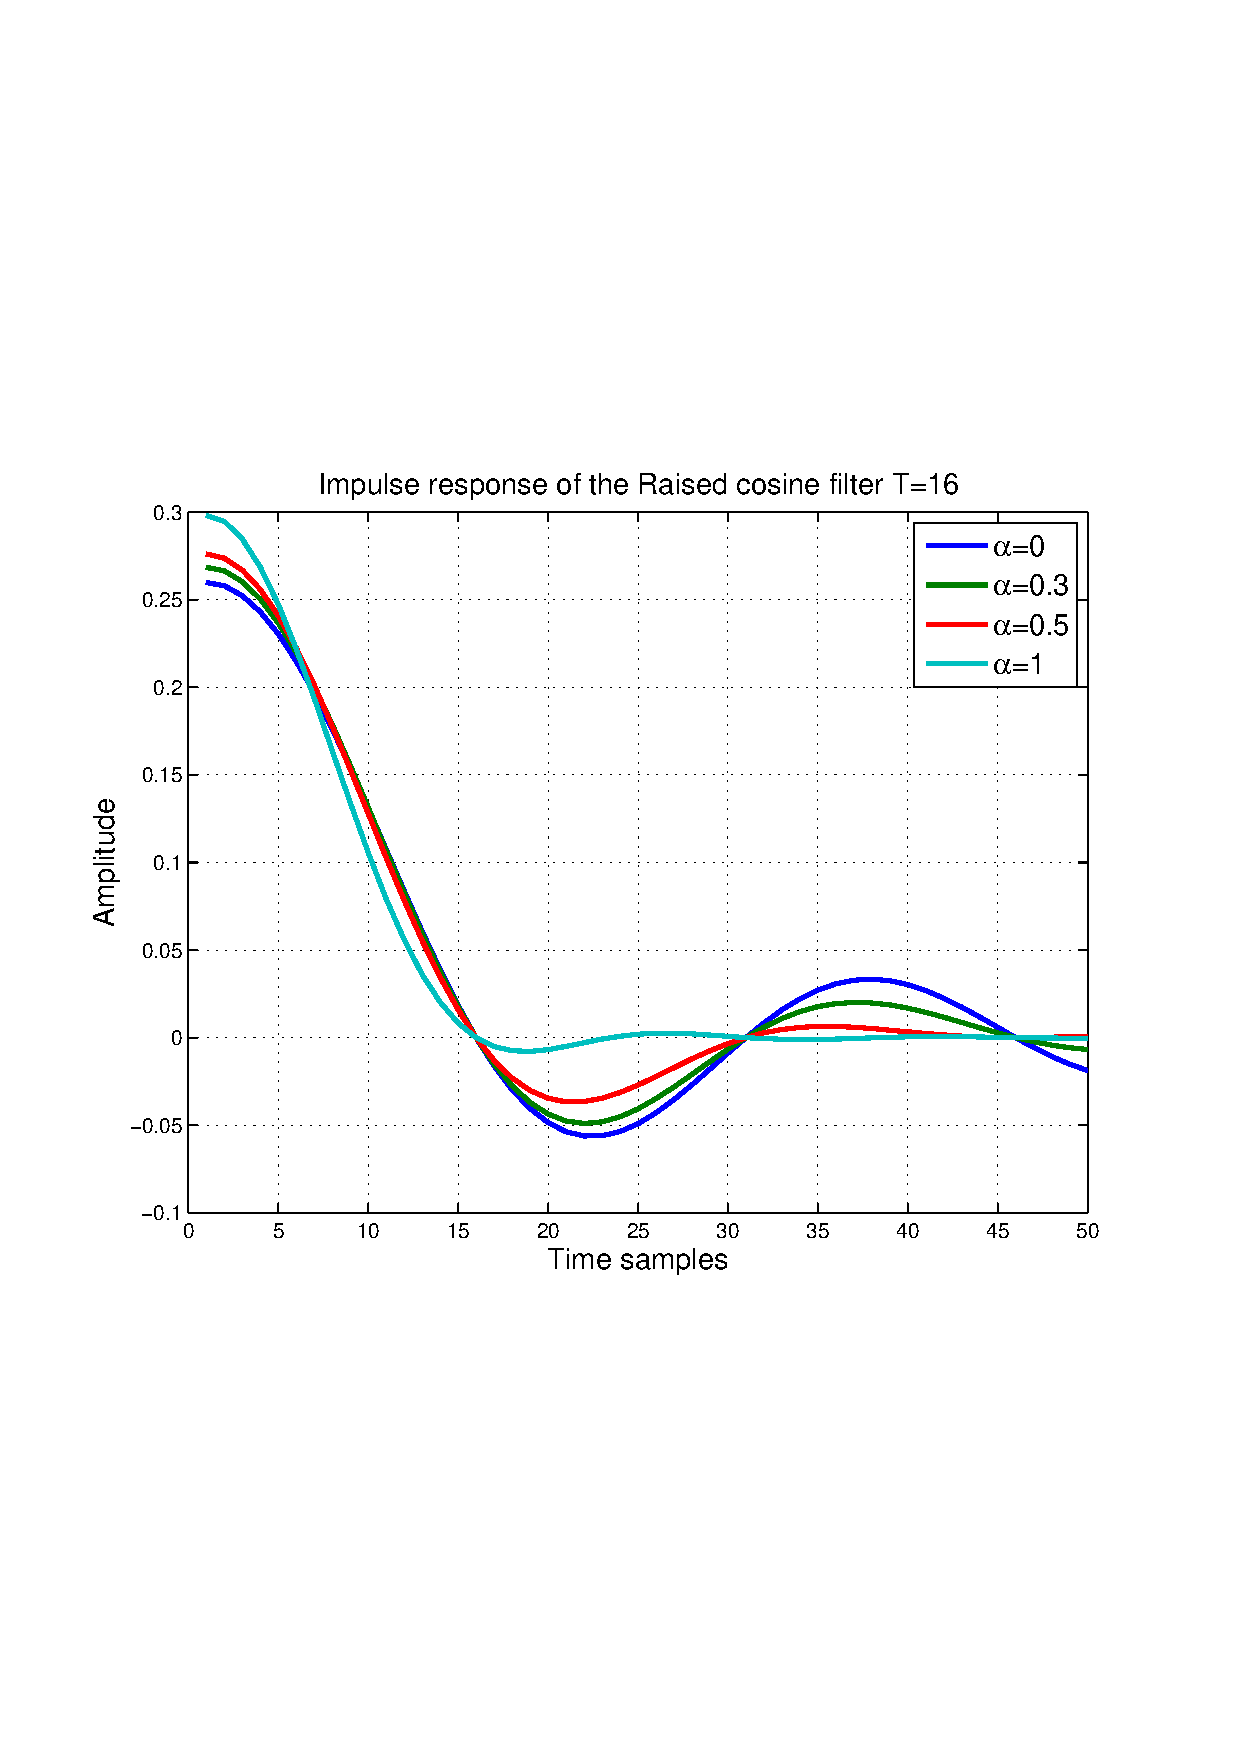
\includegraphics[width=0.9\columnwidth]{RC_time.png}
\caption{\textit{Импульсная характеристика фильтра типа Приподнятый косинус в зависимости от коэффициента $\alpha$}}
\label{fg_1}
\end{figure}
\begin{figure}[H]
\centering
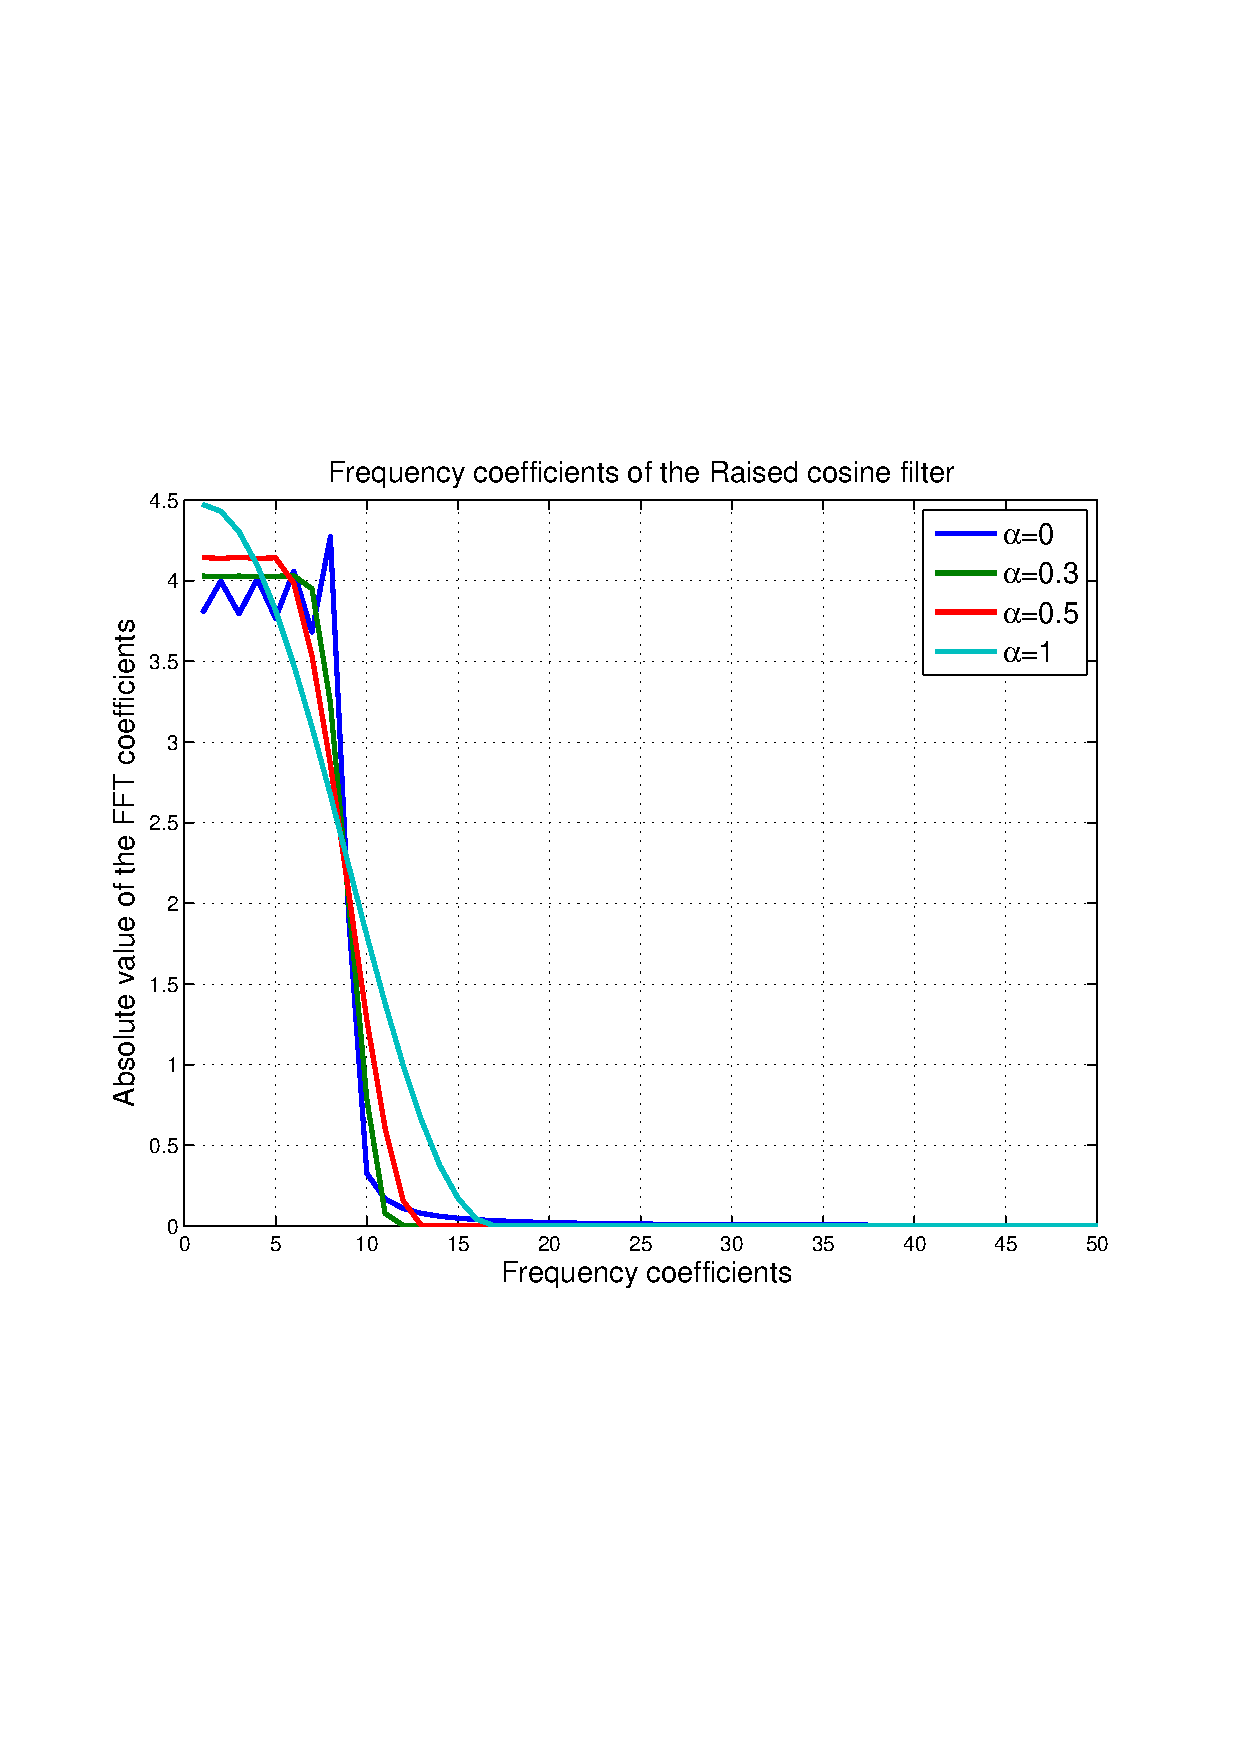
\includegraphics[width=0.9\columnwidth]{RC_freq.png}
\caption{\textit{Частотная характеристика фильтра Приподнятый косинус в зависимости от коэффициента $\alpha$}} 
\label{fg_2}
\end{figure}
Фильтр с характеристкой корень из приподнятого косинуса является дополнением к фильтру с характеристикой приподнятый косинус и при применении на приемнике и передатчике одновременно обеспечивает аналогичный уровень  межсимвольной интерференции как в согласованном фильтре. Описание и теоретическое обоснование использование фильтра описано в \cite{Book23} \cite{Book44} и \cite{Book51}. Выражение для импульсной характеристики представлено в \eqref{g_2} и взято из источника \cite{Book23}. В выражении переменная $T$ является длительностью одного символа в шкале временных отсчетов, $\alpha$ как и было описано является переменной. Импульсная характеристика для для различных величин $\alpha$ представлена на рис. Соответствующая частотная характеристика для величин $\alpha$ представлена на рис \eqref{fg_3}. 
\begin{figure}[H]
\centering
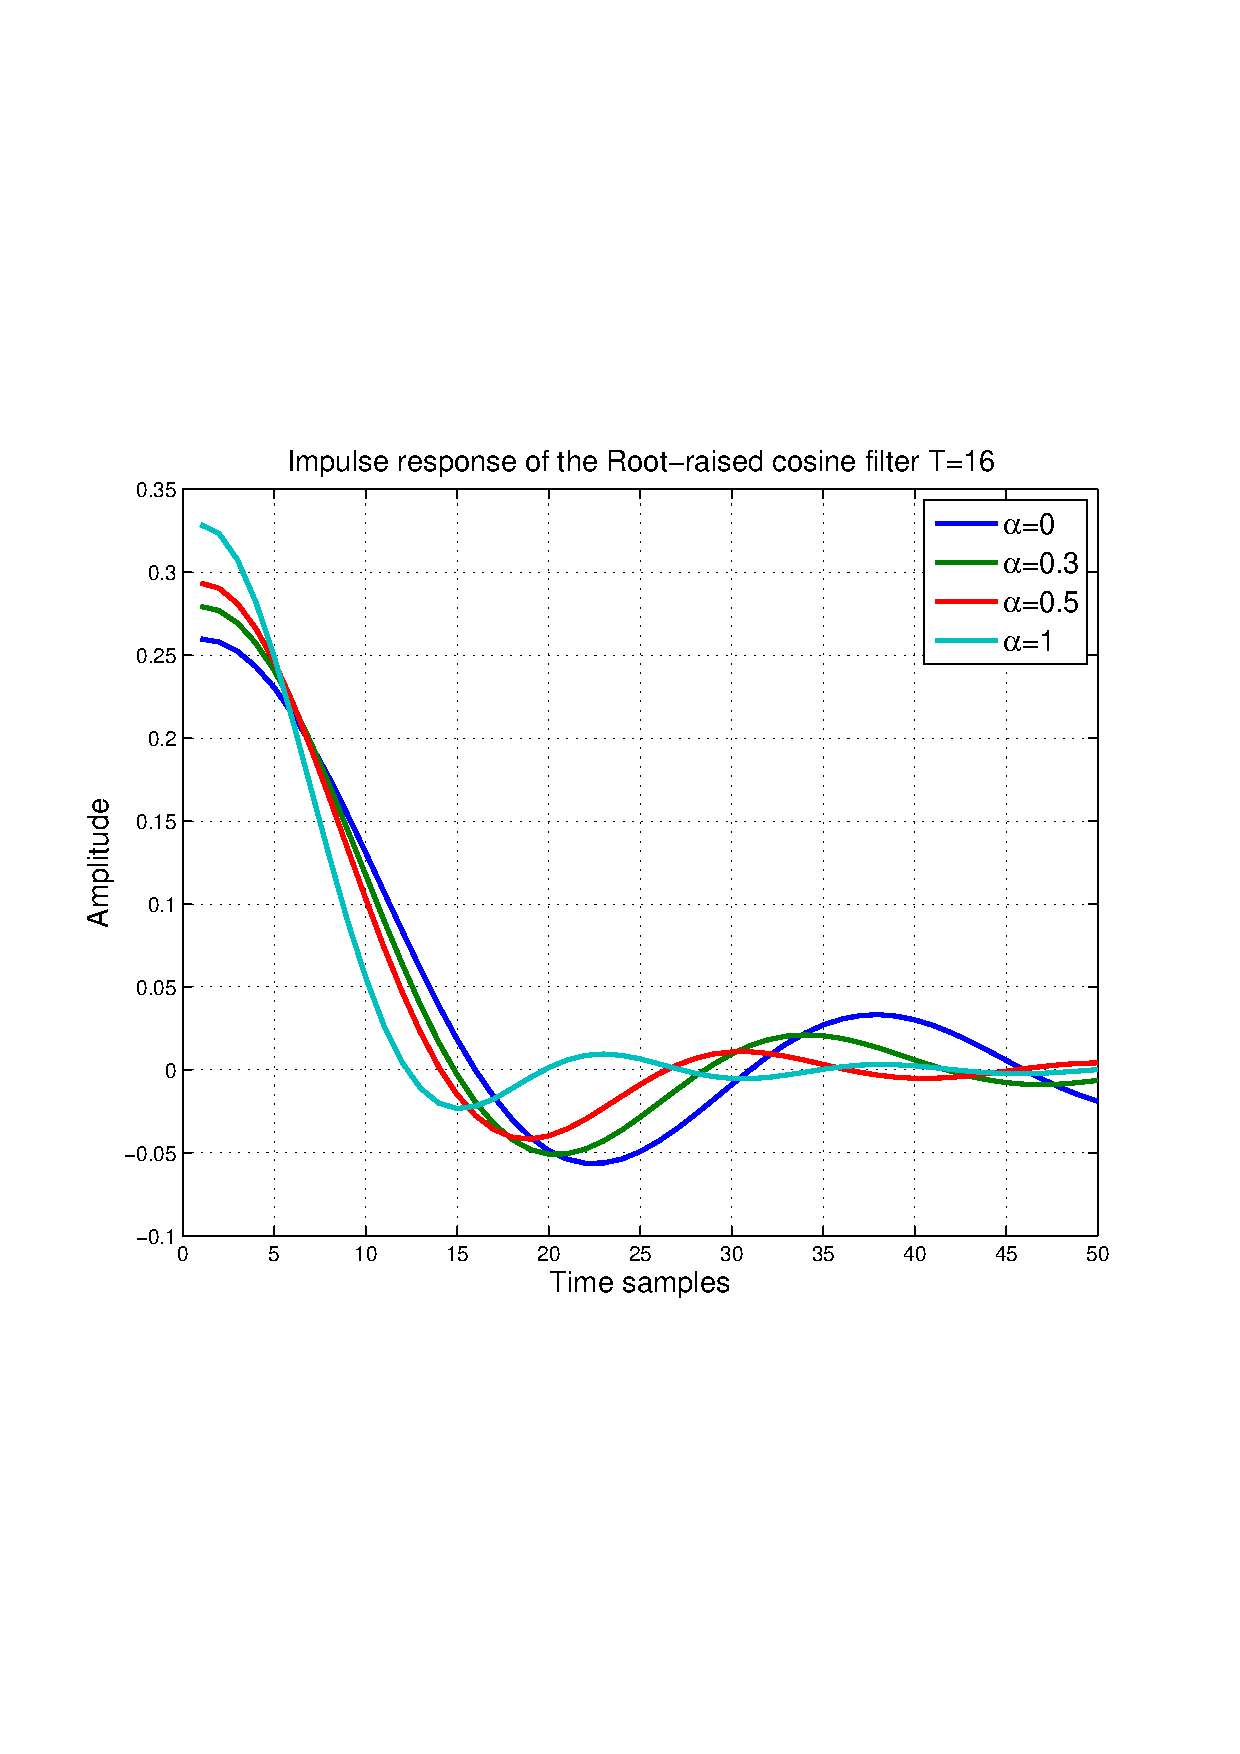
\includegraphics[width=0.9\columnwidth]{RRC_time.png}
\caption{\textit{Импульсная характеристика фильтра типа корень из Приподнятого косинуса в зависимости от коэффициента $\alpha$}} \label{fg_3}
\end{figure}
\begin{figure}[H]
\centering
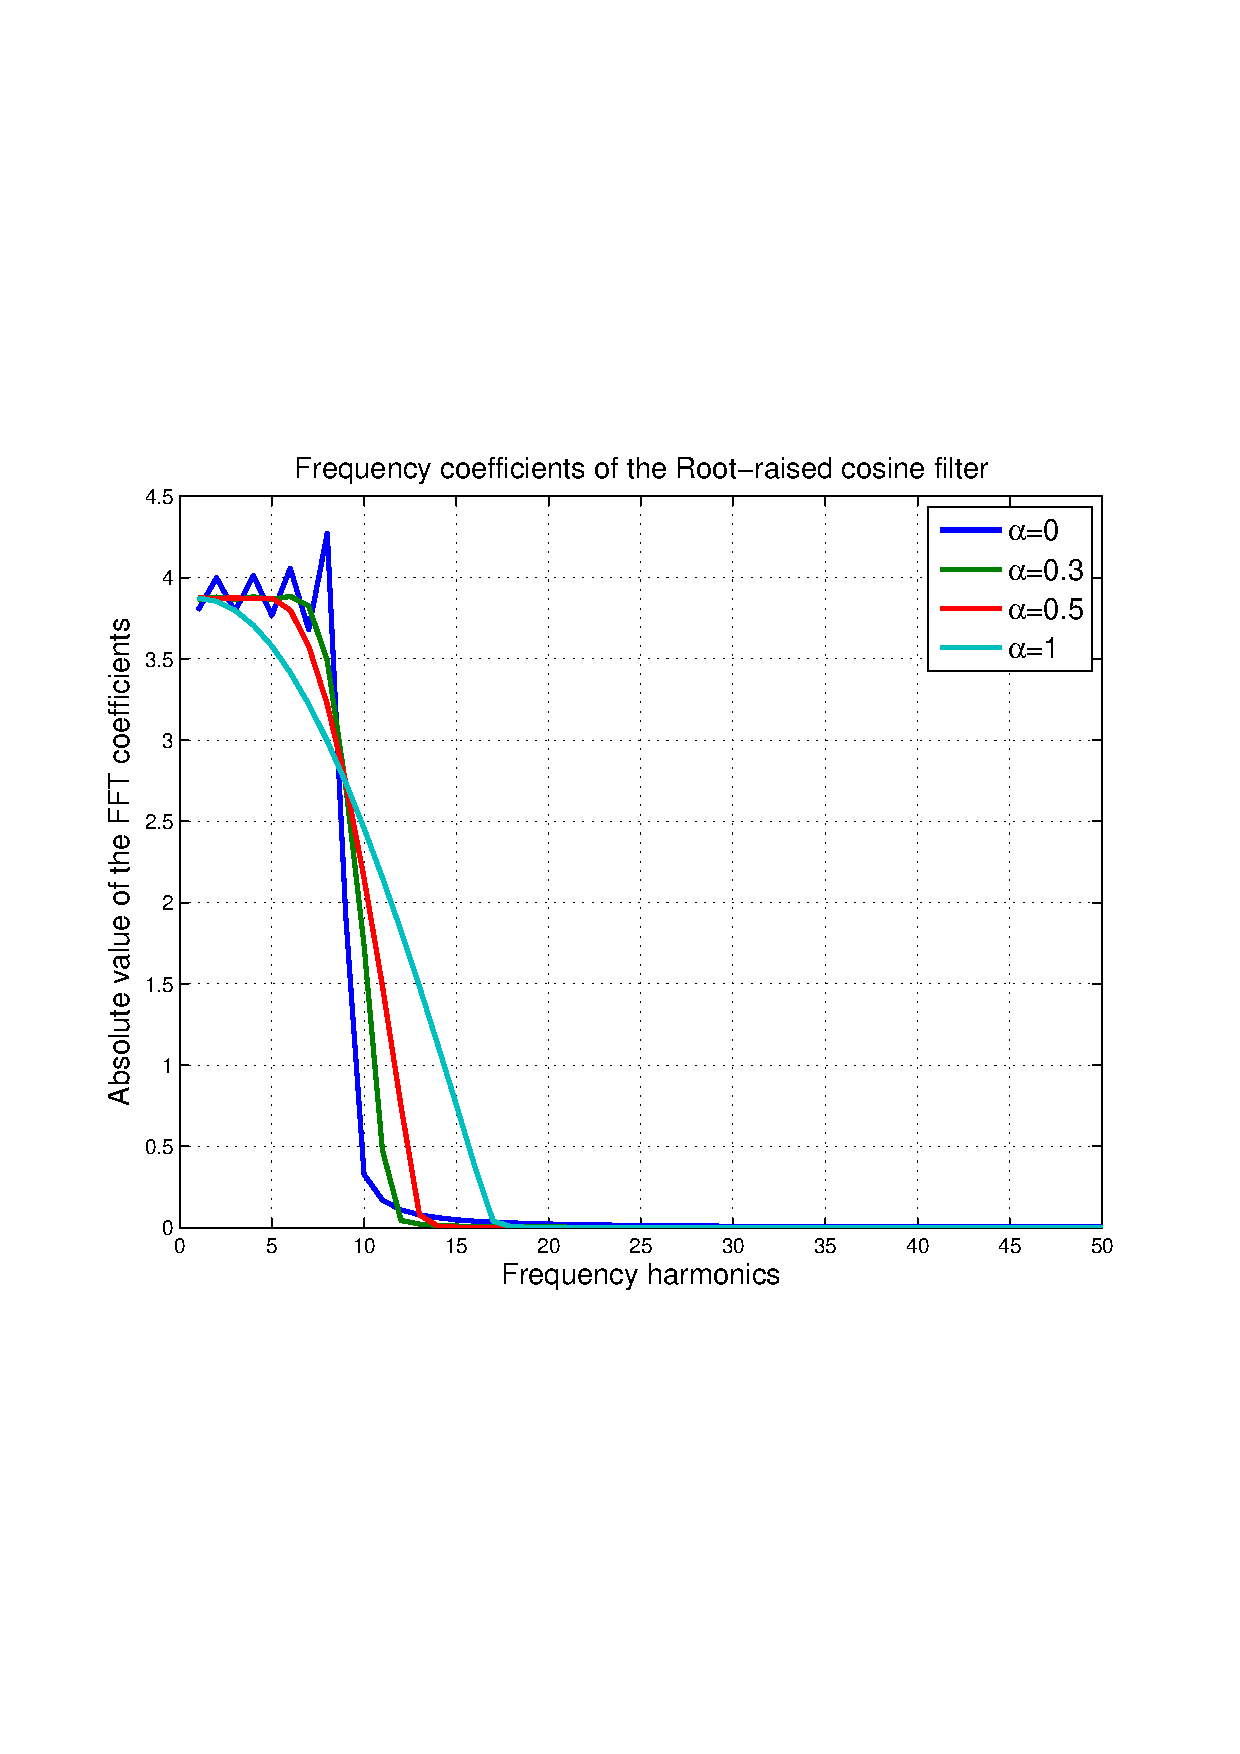
\includegraphics[width=0.9\columnwidth]{RRC_freq.png}
\caption{\textit{Частотная характеристика фильтра корень из Приподнятого косинуса в зависимости от коэффициента $\alpha$}} \label{fg_4}
\end{figure}
\begin{align}
\begin{matrix}
h(t) &=& \left\{ \begin{matrix} 
\frac{1-\alpha +4\alpha/\pi}{\sqrt{T}}& if& t=0\\
\frac{\alpha}{\sqrt{2T}}[(1+\frac{2}{\pi})sin(\frac{\pi}{4\alpha})+(1-\frac{2}{\pi})cos(\frac{\pi}{4\alpha})] & if &t= \pm T/4\alpha\\
\frac{1}{\frac{t\pi}{\sqrt{T}}(1-\frac{4*\alpha t}{T})^2}(sin(\frac{\pi t (1-\alpha)}{T})+\frac{4\alpha t}{T} cos(\frac{\pi t (1+ \alpha)}{T}) ) &otherwise \\
\end{matrix} \right.
\end{matrix}
\label{g_2}
\end{align}
Сравнение импульсных характеристик для согласованного фильтра, фильтра "Приподнятый косинус" и фильтра корень из приподнятого косинуса представлено на рис. Из рис.\eqref{fg_5} видно, что в точке где временной отсчет равен длительности импульса для согласованного фильтра амплитуда импульсной характеристики равна нулю, в отличие от других фильтров. Сравнение частотных характеристик для согласованного фильтра, фильтра "Приподнятый косинус" и фильтра корень из приподнятого косинуса представлено на рис. Из рис. видно, что для фильтра с характеристикой корень из приподнятого косинуса перекрытие по частоте является наибольшим в отличие от согласованного фильтра и фильтра с приподнятым косинусом.
\begin{figure}[H]
\centering
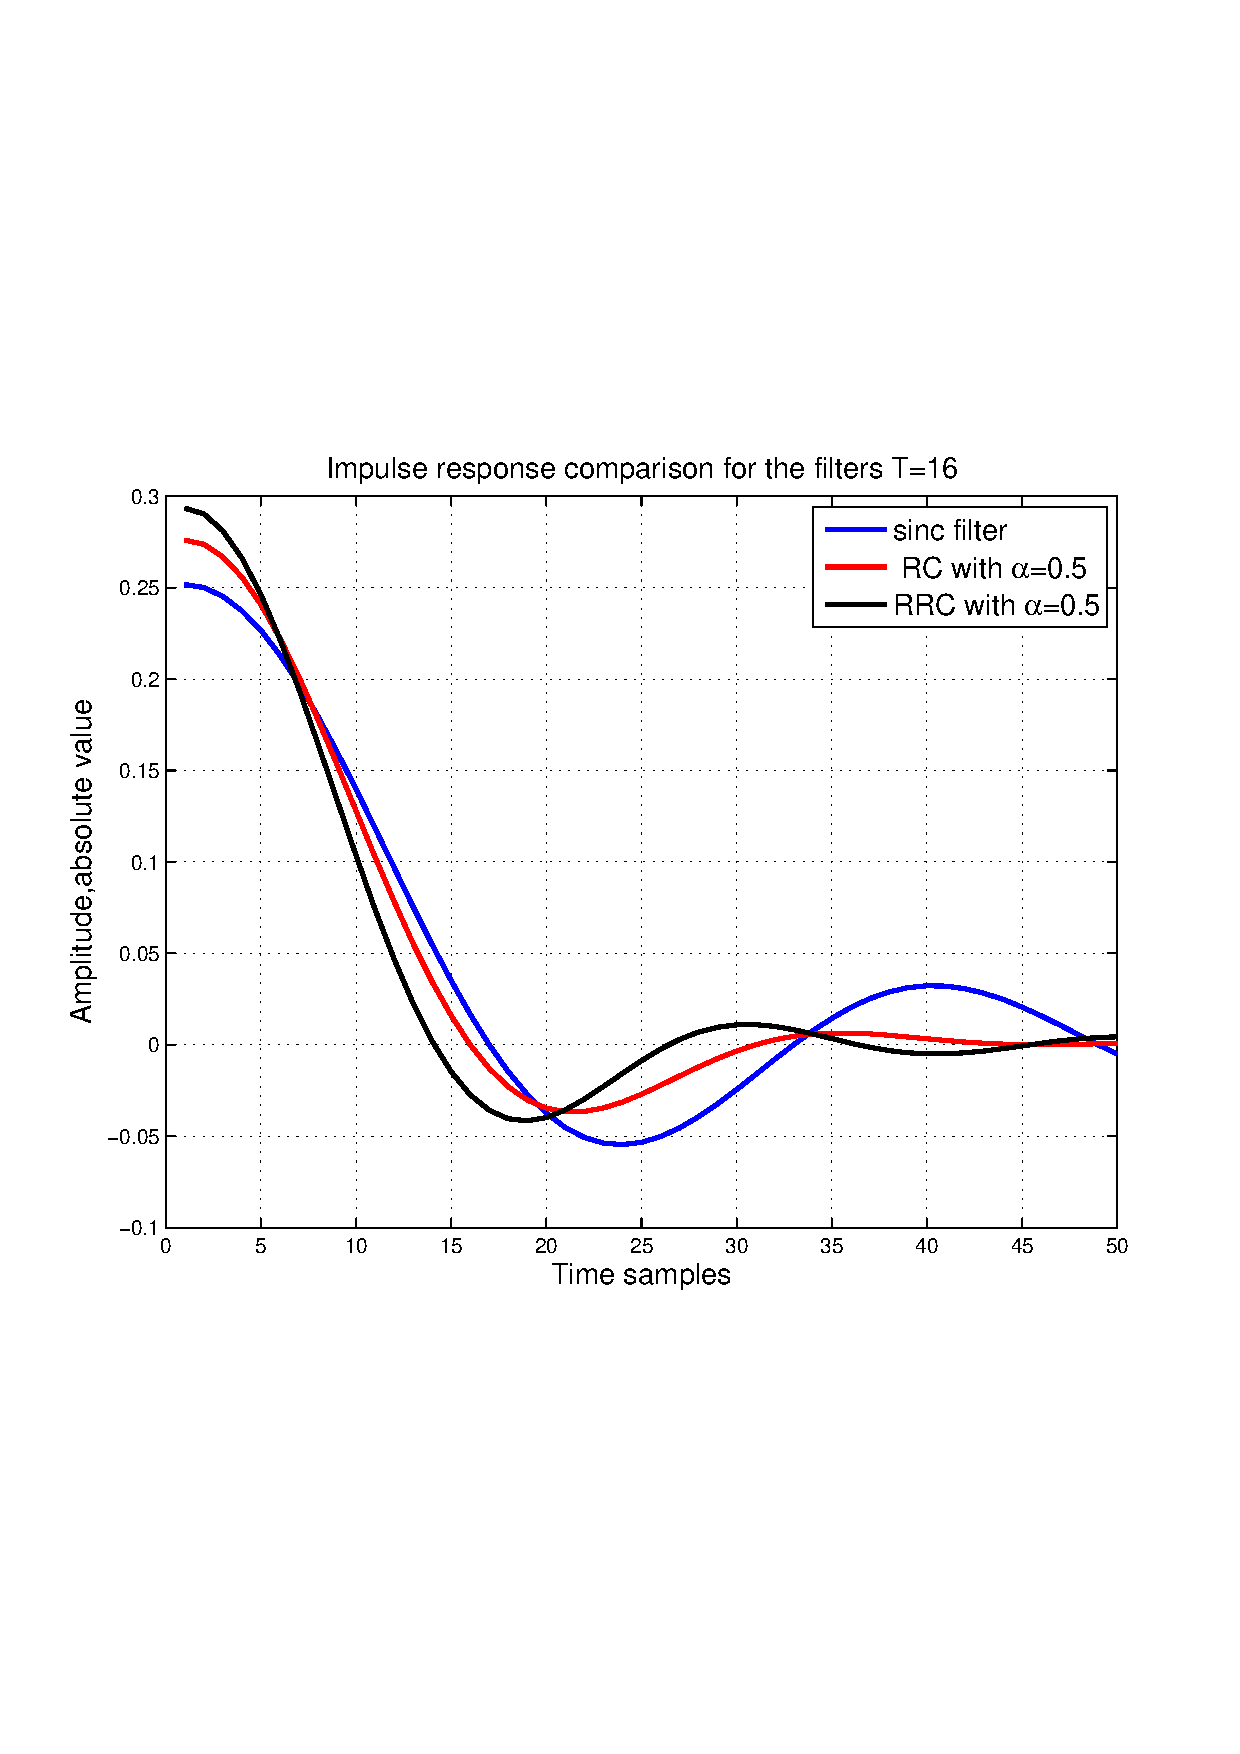
\includegraphics[width=0.9\columnwidth]{TIME_comp.png}
\caption{\textit{Сравнение импулсьных характеристик различных фильтров}} \label{fg_5}
\end{figure}
\begin{figure}[H]
\centering
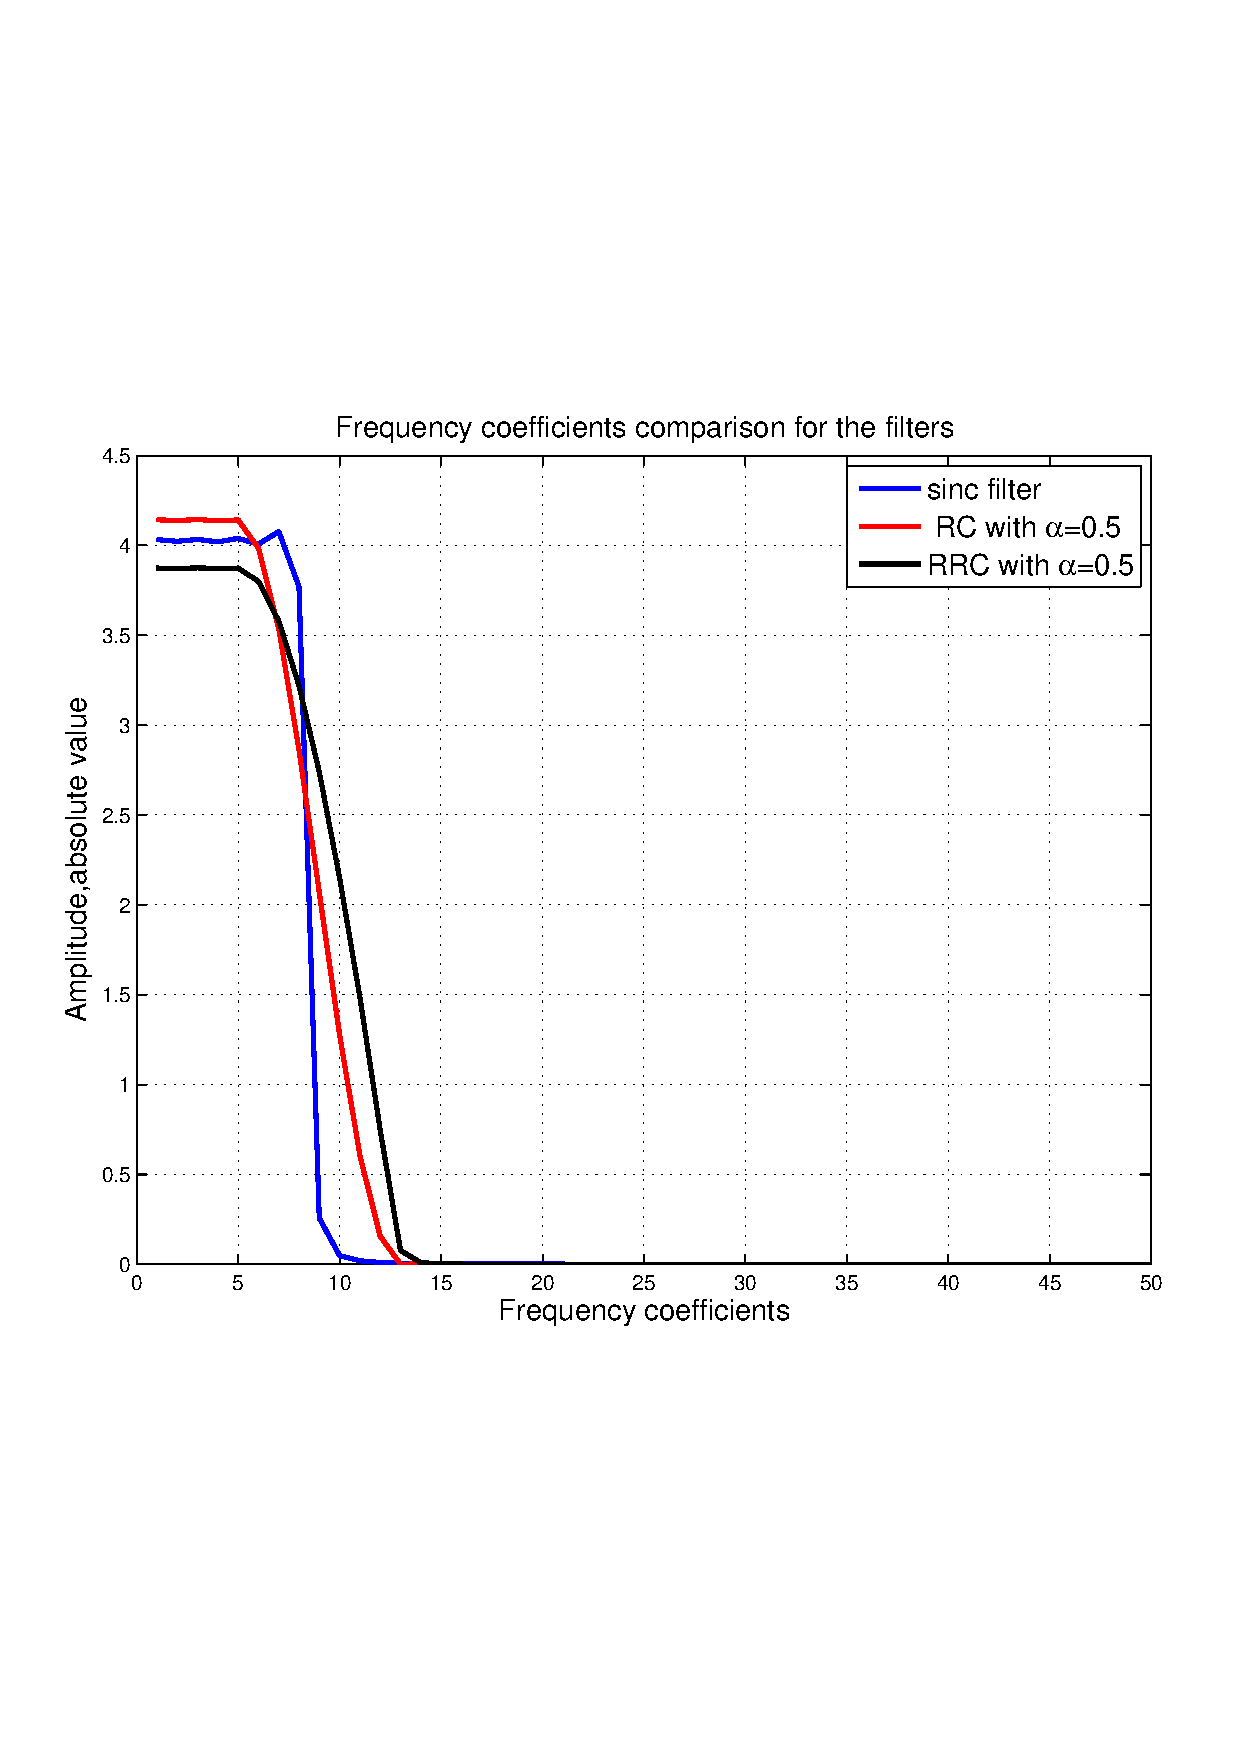
\includegraphics[width=0.9\columnwidth]{FREQ_comp.png}
\caption{\textit{С}} \label{fg_6}
\end{figure}
\clearpage
\chapter{ОбЧРК в системе с одной передающей и одной приемной антенной}
\section{Модель системы}
В данном разделе будет рассмотрена модель системы ОбЧРК. Была рассмотрена система передачи с воздействием канала. Канал в физическом смысле полагается как компоненты многолучевого распространения между передатчиком и приемником\cite{}. Так же канал может быть описан как свертка между переданным сигналом и некоторой импульсной характеристикой. В таком случае поступивший на вход приемника сигнал может быть описан следующим образом \eqref{siso_1}, где $y$ является вектором поступивших на вход приемника данных, $x$ это вектор переданных с выхода передатчика данных и $H$ это матрица свертки между входными данными и некоторой импульсной характеристикой. При этом переданный с выхода передатчика сигнал может быть связан с передаваемыми символами при помощи модели $PARATUCK2$ и ее двумя формами записи в векторизированной форме \eqref{siso_2}\eqref{siso_3}\cite{Book21}. 
\begin{align}
\mathbf{y}=\mathbf{Hx}
\label{siso_1}
\end{align}
\begin{align*}
\mathbf{y,x}\in\compl^{T\times 1}
\mathbf{H}\in\compl^{T\times T}
\end{align*}
\begin{align}
\mathbf{x}=\mathcal{X}_{[3]}=vec(\mathcal{X})=\mathbf{\Omega}_1 vec(\mathbf{S})
\label{siso_2}
\end{align}
\begin{align*}
\mathbf{\Omega}_1 \in \compl^{T\times T_s \cdot F}
\end{align*}
\begin{align}
\mathbf{\Omega}_1=(\mathbf{C}^{[b]T}\diamond \mathbf{C}^{[a]T})^T \diamond (\mathbf{b^T \otimes a}) \
\end{align}
\begin{align}
\mathcal{X}_{:,:,i}=\mathbf{a}\cdot diag(\mathbf{C}^{[a]}_{:,i})\cdot \mathbf{S} \cdot diag(\mathbf{C}^{[b]}_{:,i}) \cdot \mathbf{b} \label{siso_3}
\end{align}
Переданные данные могут быть сгенерированы при помощи модели $PARATUCK2$ третьего порядка в векторизованной форме или развертке третьего измерения. В таком случае матрица символов передаваемых при помощи системы передачи ОбЧРК будет записана как матрица основа $\mathbf{S}$ в модели $PARATUCK2$\cite{Book6}\eqref{siso_4}\eqref{siso_5}. Таким образом можно без изменений внести все символы в систему передачи. 

Каждый столбец в $\Camat$ матрице соответствует определенной поднесущей частоте для модуляции. Таким образом матрица $\Camat$ конструируется как значения поднесущих частот в каждом из столбцов. Таким образом матрица $\Camat$ может быть записана следующим образом \eqref{siso_1}.
 \begin{align}
 c^{[a]}_{t,f}=e^{-j2\pi\cdot(t\cdot f)/T_s} \label{siso_4}
 \end{align}
\begin{align}
\mathbf{C}^{[a]}=\begin{bmatrix}
e^{-j2\pi\cdot 0}& e^{-j2\pi\cdot 0}& \cdots & e^{-j2\pi\cdot 0} \\
e^{-j2\pi\cdot 0}& e^{-j2\pi\cdot 1/T_s}& \cdots &e^{-j2\pi\cdot F/T_s} \\
e^{-j2\pi\cdot 0}& e^{-j2\pi\cdot 2/T_s}& \cdots &e^{-j2\pi\cdot 2F/T_s} \\
&&\vdots \\
e^{-j2\pi\cdot 0}& e^{-j2\pi\cdot T/T_s}& \cdots & e^{-j2\pi\cdot T\cdot F /T_s} \\
\end{bmatrix} \label{siso_5}
\end{align}
Каждый столбец матрицы $\Cbmat$ определяет функцию фильтрации во временной области для заданного блока данных. Столбцы являются сдвинутыми версиями первого столбца. Сдвиг между соседними столбцами равен $T/T_s$\eqref{siso_7}. Элементы в столбце определяются по следующему выражению \eqref{siso_6}\cite{Book12}. При конструировании матрицы $\Cbmat$ задается коэффициент перекрытия $\alpha$.
\begin{align}
\begin{matrix}
u(t) &=& \left\{ \begin{matrix} 
\frac{1-\alpha +4\alpha/\pi}{\sqrt{T}}& if& t=0\\
\frac{\alpha}{\sqrt{2T}}[(1+\frac{2}{\pi})sin(\frac{\pi}{4\alpha})+(1-\frac{2}{\pi})cos(\frac{\pi}{4\alpha})] & if &t= \pm T/4\alpha\\
\frac{1}{\frac{t\pi}{\sqrt{T}}(1-\frac{4*\alpha t}{T})^2}(sin(\frac{\pi t (1-\alpha)}{T})+\frac{4\alpha t}{T} cos(\frac{\pi t (1+ \alpha)}{T}) ) &otherwise \\
\end{matrix} \right.
\end{matrix}\label{siso_6}
\end{align}
\begin{align}
\mathbf{C}^{[b]}=\begin{bmatrix}
\mathbf{u}_{0}& \mathbf{u}_{1}& \cdots &\mathbf{u}_{T_s}\\
\end{bmatrix} \label{siso_7}
\end{align}
Матрица $\Bmat$ при моделировании ОбЧРК становится столбцом $\bmat$ и в физическом смысле соответствует изменению по амплитуде между символами на различных временных позициях\cite{Book34}. Поскольку мы рассматриваем линейную независимую от времени систему то все значения в столбце равны единице. Кроме того таким образом можно выразить различные взвешивающие коэффициенты позволяющие не передавать символы по определенным временным позициям\eqref{siso_8}.
\begin{align}
\mathbf{b}=\mathbf{1}_{T_s\times 1} \label{siso_8}
\end{align}
\begin{align}
\mathbf{b}\in \real^{T_s\times 1} \label{siso_9}
\end{align}
Матрица $\Amat$ при моделировании GFDM становится строкой $\amat$ и в физическом смысле соответствует коэффициентам передачи для каждой поднесущей в течении одного блока передачи. В данной работе будет рассмотрена система где значения а могут быть структурированы двумя образами\eqref{siso_10}. В первом случае строка а имеет все единичные значения. Во втором случае величины в строке а могут быть распределены случайным образом между значениями $1$ и $0$. Так же при помощи строки $\amat$ может быть   аппроксимировано влияние канала. Однако точность такой аппроксимации мала.
\begin{align}
\mathbf{a}=\mathbf{1}_{1\times F} \label{siso_10}
\end{align}
\begin{align}
\mathbf{a}\in \compl^{1\times F} \label{siso_11}
\end{align}
Определив указанным образом соответствующие матрицы, сигнал на выходе передатчика может быть определен при помощи одного из последующих выражений \eqref{siso_13} \eqref{siso_14}. При этом модель системы ОбЧРК может быть совпадает с тензорной моделью $PARATUCK2$.
\begin{align}
\mathbf{x}^T=\mathbf{a}\cdot (\mathbf{C}^{[a]T} \odot (\mathbf{S}\cdot (\mathbf{C}^{[b]}\diamond \mathbf{b}^T)^T)) \label{siso_12}
\end{align}
\begin{align}
\mathbf{x}=((\mathbf{a}\diamond \mathbf{C}^{[a]})^T \cdot \mathbf{S}) \odot \mathbf{C}^{[b]} \mathbf{b}) \label{siso_13}
\end{align}
\begin{align}
\mathbf{x}=((\mathbf{b}^T\diamond \mathbf{C}^{[b]})^T \cdot \mathbf{S}^T) \odot \mathbf{C}^{[a]T} \mathbf{a}^T) \label{siso_14}
\end{align}
\begin{align*}
\mathbf{x} \in \compl^{T\times 1 }
\mathbf{a} \in \compl^{1\times F}
\mathbf{C}^{[a]} \in \compl^{T\times  F}
\end{align*}
\begin{align*}
\mathbf{C}^{[b]} \in \compl^{T \times T_s}
\mathbf{b} \in \compl^{T_s\times 1}
\mathcal{S} \in \compl^{F\times T_s }
\end{align*}
\section{Канал с аддитивным белым гауссовым шумом}
В данной секции будет рассмотрена модель системы в которой канал отсутствует, либо его влияние устранено.  В таком случае матрица $H$  из матрицы свертки преобразуется в единичную матрицу\cite{Book30}, а модель будет описана при помощи следующего выражения \eqref{siso_15}. Для подобного рода систем существует два классических решения.
\begin{align}
\mathbf{y}=\mathbf{\Omega}_1vec(\mathbf{S})+\mathbf{n} \label{siso_15}
\end{align}
\begin{align*}
\mathbf{\Omega}_1 \in \compl^{T\times T_s \cdot F}
\end{align*}
\begin{align}
\mathbf{\Omega}_1=(\mathbf{C}^{[b]T}\diamond \mathbf{C}^{[a]T})^T \diamond (\mathbf{b \otimes a})
\end{align}
\begin{align*}
\mathbf{y,n}\in \compl^{1\times T}
\mathbf{S}\in \compl^{F\times T_s}
\end{align*}
\begin{align*}
\mathbf{a} \in \compl^{1\times F}
\mathbf{C}^{[a]} \in \compl^{T\times  F}
\mathbf{C}^{[b]} \in \compl^{T \times T_s}
\mathbf{b} \in \compl^{T_s\times 1}
\end{align*}
\subsection{Приемник на основе псевдообратной матрицы}
Первое решение заключается оптимального решения с точки зрения второй нормы\cite{Book11}.  Для начала введем матрицу $\mathbf{\Omega}_1$ которая будет выражать взаимосвязь между векторизированной матрицей символов и сигналом на выходе передатчика\eqref{siso_ls_1}. Данное выражение может быть выведено из \eqref{siso_ls_3}. Приемник может найти наилучшие значения переданных данных при помощи решения задачи оптимизации\cite{Book26}. В таком случае может быть составлена следующая функция невязки \eqref{siso_ls_4}. Поскольку используется вторая норма, решение данной задачи существует и оно единственно. В случае если векторы а и б имеют структуру со всеми единицами мы можем ими пренебречь. Тогда матрица $\Omega$ будет записана как произведение Хатри-Рао между матрицами $\Camat$ и $\Cbmat$\eqref{siso_ls_4}.
\begin{align}
vec(\mathbf{x})=\mathbf{\Omega}_1\cdot vec(\mathbf{\widehat{S}}) \label{siso_ls_1}
\end{align}
\begin{align*}
\mathbf{\Omega}_1 \in \compl^{T\times T_s \cdot F}
\end{align*}
%\mathbf{\Omega}_3 \in \compl^{T\times T_s}
%\mathbf{\Omega}_2 \in \compl^{T\times F}
%vec(\mathbf{a}) \in \compl^{F \times 1}
\begin{align*}
vec(\mathbf{\widehat{S}}) \in \compl^{F \cdot T_s \times 1}
\end{align*}
\begin{align}
\mathbf{\Omega}_1=(\mathbf{C}^{[b]T}\diamond \mathbf{C}^{[a]T})^T \diamond (\mathbf{b \otimes a}) \label{siso_ls_2}
\end{align}
\begin{align}
\mathbf{\Omega}_1=(\mathbf{C}^{[b]T}\diamond \mathbf{C}^{[a]T})^T  \label{siso_ls_3}
\end{align}

\begin{align}
r_1= \mathbf{y}-\mathbf{\Omega}_1 \cdot vec(\mathbf{\widehat{S}})  \label{siso_ls_4}
\end{align}

Для того чтобы найти оптимальное решение возьмем первую производную от оптимизируемой функции\eqref{siso_ls_5}\cite{Book24}. Поскольку она комплексна и не аналитична, используем  исчисление Виртингера\eqref{siso_ls_6}, для того чтобы взять производную по комплексно сопряженной от переменной. Приравняем первую производную нулю и решим задачу используя псевдообратную матрицу\eqref{siso_ls_10}\cite{Book24}.
\begin{align}
\min_{vec(\mathbf{\widehat{S}})} r_1^H\cdot r_1=\min_{vec(\mathbf{\widehat{S}})} \mid\mid r_1\mid\mid^2  \label{siso_ls_5}
\end{align}
\begin{align}
r_1^H\cdot r_1=(vec(\mathbf{y})-\mathbf{\Omega}_1 \cdot vec(\mathbf{\widehat{S}}))^H\cdot(vec(\mathbf{y})-\mathbf{\Omega}_1 \cdot vec(\mathbf{\widehat{S}}))  \label{siso_ls_6}
\end{align}
\begin{align*}
r_1^H\cdot r_1=\mid\mid vec(\mathbf{y})\mid\mid^2 + vec(\mathbf{\widehat{S}})^H\mathbf{\Omega}_1^H \mathbf{\Omega}_1 vec(\mathbf{\widehat{S}}) 
\end{align*}
\begin{align}
-vec(\mathbf{y})^H \mathbf{\Omega}_1 vec(\mathbf{\widehat{S}})- vec(\mathbf{\widehat{S}})^H\mathbf{\Omega}_1^Hvec(\mathbf{y}) \label{siso_ls_7}
\end{align}
\begin{align}
\frac{\delta r_1^H\cdot r_1}{\delta vec(\mathbf{\widehat{S}}^*)} = \mathbf{\Omega}_1^H \mathbf{\Omega}_1 vec(\mathbf{\widehat{S}}) -\mathbf{\Omega}_1^Hvec(\mathbf{y})=0  \label{siso_ls_8}
\end{align}
\begin{align}
\mathbf{\Omega}_1^H \mathbf{\Omega}_1 vec(\mathbf{\widehat{S}})=\mathbf{\Omega}_1^Hvec(\mathbf{y}) \label{siso_ls_9}
\end{align}
\begin{align}
vec(\mathbf{\widehat{S}})_{opt}= (\mathbf{\Omega}_1^H \mathbf{\Omega}_1)^{-1}\mathbf{\Omega}_1^Hvec(\mathbf{y})  \label{siso_ls_10}
\end{align}
\subsection{Приемник на основе согласованного фильтра}
Существует другое решение задачи обеспечивающее более стабильное решение. Псевдообратная матрица имеет значительный недостаток в случае если матрица для которой осуществляется инверсия имеет плохое число обусловленности\cite{Book25}\eqref{siso_mf_1}. В таком случае если в принятых данных присутствует белый гауссов шум, его компоненты будут увеличены по мощности, что приведет к уменьшение соотношения $SNR$. Это можно легко увидеть используя разложение матрицы на собственные значения\eqref{siso_mf_2}\cite{Book25}. В таком случае обратная матрица к исходной будет записана следующим образом \eqref{siso_mf_4}. Как видно из выражения \eqref{siso_mf_4} при умножении вектора шума на матрицу обратную к $\mathbf{\Omega}_1$ происходит умножение собственных значений шума на  величины обратные к собственным значениям матрицы $\mathbf{\Omega}_1$\eqref{siso_mf_5}\cite{Book24}. Таким образом значения имеющие маленькую величину в обратной матрице обеспечат увеличение компонент шума\cite{}. Для того чтобы избежать подобного влияния можно произвести умножение на эрмитово сопряженную матрицу с исходной. В таком случае соотношение $SNR$ останется неизменным\eqref{siso_mf_6}. 
\begin{align}
\mathbf{\Omega}_1=\mathbf{U\Sigma V^H} \label{siso_mf_1}
\end{align}
\begin{align}
\mathbf{\Omega}_1^{-1}=\mathbf{V\Sigma^{-1} U^H} \label{siso_mf_2}
\end{align}
\begin{align}
\mathbf{n}=\mathbf{U I\delta^2 V^H} \label{siso_mf_3}
\end{align}
\begin{align}
E(\mathbf{\Omega}_1^{-1}\mathbf{n})=\mathbf{V(\Sigma^{-1}\cdot I\delta^2) V^H} \label{siso_mf_4}
\end{align}
\begin{align}
\mathbf{\Omega}_1^{H}=\mathbf{V\Sigma U^H} \label{siso_mf_5}
\end{align}
\begin{align}
E(\mathbf{\Omega}_1^{H}\mathbf{n})=\mathbf{V(\Sigma\cdot I\delta^2) V^H} \label{siso_mf_6}
\end{align}

\section{Поиск коэффициентов передачи поднесущих}
Введенные выше коэффициенты $\mathbf{a}$ используются для выбора рабочих поднесущих в системе. Изменение значений вектора $\mathbf{a}$ может быть использовано для уменьшения интерференции с другими системами работающими в том же диапазоне частот, что и система ОбЧРК\cite{Book25}.  Таким образом значение вектора $\mathbf{a}$ может быть неизвестным для приемника. Информация о коэффициенте передачи поднесущей должна быть дополнительным образом найдена на приемнике. Рассмотренная модель может быть описана при помощи модели $PARATUCK2$ третьего порядка\eqref{siso_s_1}.
\begin{align}
\mathbf{y}=\mathbf{\Omega}_1vec(\mathbf{S})+\mathbf{n} \label{siso_s_1}
\end{align}
 Тогда вектор $\mathbf{a}$ описывает коэффициент передачи каждой из поднесущей. Выражение \eqref{siso_s_2} может быть сформулировано относительно вектора $\mathbf{a}$ выписанного в правую часть. Таким образом можно записать уравнение невязки для искомого вектора $\mathbf{a}$\eqref{siso_s_3}. 
 \begin{align}
\mathbf{\Omega}_2=((\mathbf{C}^{[b]}\diamond \mathbf{b}^T)^T\cdot S^T) \odot \mathbf{C}^{[a]}   \label{siso_s_2}
\end{align}
\begin{align}
r_2= \mathbf{y}-\mathbf{\Omega}_2 \cdot vec(\mathbf{a})  \label{siso_s_3}
\end{align}

Приемник может найти как неизвестные величины вектора $\mathbf{a}$ так и переданные символы, но не в полном объеме. Поскольку в принятом на вход приемника блоке данных всего $T_s\cdot F$ величин, в то время как количество переменных равно $(T_s+1)\cdot F$ то задача является неопределенной и необходимо уменьшить количество неизвестных для решения задачи. Одним из возможных решений является определить для приемника первый символ на каждой из поднесущих, тогда количество неизвестных будет равно количество принятых на входи приемника данных и задача будет иметь как минимум одно решение. При помощи известных символов приемник сможет найти коэффициенты передачи поднесущих, после чего восстановит значения неизвестных для него символов\eqref{siso_sm_1}. Тогда для нахождения неизвестных величин должна быть сформулирована оптимизационная задача для приемника в ходе которой он сможет найти все неизвестные. Неизвестными переменными являются матрица символов $\mathbf{S}$ и вектор коэффициентов поднесущих $\mathbf{a}$. Известный символы добавлены в оптимизируемую функцию в качестве ограничения. Данный подход увеличивает вычислительную сложность задачи, однако значительно упрощает ее решение. Подобную задачу можно решить путем множителей Лагранжа. Задача была решена добавлением второй нормы от ограничения в функцию минимизации. Таким образом задача была упрощена с аналитической точки зрения однако так же усложнения с точки зрения вычислительной сложности. Кроме того было использовано два подхода по рассмотрению связи между невязками $r_1$ и $r_2$. Мы рассматривали как равенство функций $r_1$ и $r_2$ в той же самой точке, как и отсутствие связи между ними. В случае если связь отсутствует, производная по $\mathbf{S}$ и $\mathbf{a}$ равна нулю. В случае если связь присутствует производная по $\mathbf{S}$ и $\mathbf{a}$  не равна нулю.Далее будут рассмотрены оба подхода к решению оптимизационной задачи.
\subsection{Приближенный полу-слепой приемник}
Описанный ниже способ решения подразумевает отсутствие связи между $r_1$ и $r_2$. Постановка задачи записана в выражении \eqref{siso_sm_2}. Происходит минимизация функции с предположением что две оптимизируемые функции не зависят друг от друга.
\begin{align*}
\mathbf{r}_1= vec(\mathbf{y})-\mathbf{\Omega}_1 \cdot vec(\mathbf{\widehat{S}})
\end{align*}
 Функция невязки $r_1$ соответствует оптимизируемой функции относительно символов.  Матрица $\mathbf{\Omega}_1$ была определена ранее.
Функция невязки $r_2$ соответствует оптимизируемой функции относительно коэффициентов поднесущих. Матрица $\mathbf{\Omega}_2$ была определена ранее и соответствует переданным данным с выраженными из матрицы коэффициентами поднесущих.
 \begin{align*}
\mathbf{r}_2=vec(\mathbf{y})-\mathbf{\Omega}_2 \cdot vec(\mathbf{\widehat{s}})
\end{align*}
Функция невязки соответствует поставленному для алгоритма ограничению. В качестве матрицы выбора использована матрица $\mathbf{S}_{sel}$. В матрице $\mathbf{S}_{sel}$ присутствуют элементы только на главной диагонали и только в тех строках для которых переданный символ известен. Так же матрицу можно получить другим способом при помощи выражения.

 Вектор $\mathbf{q}$ является вектором где присутствуют известные символы, при этом от имеет ту же размерность что и вектор символов и на неизвестных позициях элементы равны нулю.
 \begin{align}
\mathbf{r}_3=\mathbf{q} -\mathbf{S}_{sel} vec(\mathbf{\widehat{S}}); \label{siso_sm_1}
\end{align}
\begin{align*}
\mathbf{S}_{sel}=diag(\mathbf{q})^{-1}diag(\mathbf{q})
\end{align*}
\begin{align*}
\mathbf{q}\in \compl^{T_s \cdot F\times 1}
\mathbf{S}_{sel}\in \compl^{T_s \cdot F\times T_s \cdot F} 
\end{align*}
\begin{align*}
\mathbf{r}_1 \in \compl^{T_s \cdot F \times 1}
\mathbf{r}_2 \in \compl^{F \times 1}
\mathbf{r}_3 \in \compl^{T_s \cdot F \times 1}
\end{align*}
\begin{align}
\min_{vec(\mathbf{\widehat{S}})} r_1^Hr_1 \label{siso_sm_2}
\end{align}
\begin{align}
\min_{vec(\mathbf{a})} r_2^Hr_2 \label{siso_sm_3}
\end{align}
\begin{align}
\min_{vec(\mathbf{\widehat{S}})} r_3^Hr_3 \label{siso_sm_4}
\end{align}
\begin{align}
\begin{bmatrix}
\frac{\delta \mathbf{r}_1^H \mathbf{r}_1}{\delta vec(\mathbf{\widehat{S}})^*}\\
\frac{\delta \mathbf{r}_2^H \mathbf{r}_2}{\delta vec(\mathbf{\widehat{a}})^*}\\
\frac{\delta \mathbf{r}_3^H \mathbf{r}_3}{\delta vec(\mathbf{\widehat{S}})^*}\\
\end{bmatrix}=
\begin{bmatrix}
0\\
0\\
0\\
\end{bmatrix} \label{siso_sm_5}
\end{align}
\begin{align}
\begin{bmatrix}
\frac{\delta \mathbf{r}_1^H \mathbf{r}_1}{\delta vec(\mathbf{\widehat{S}})^*}\\
\frac{\delta \mathbf{r}_2^H \mathbf{r}_2}{\delta vec(\mathbf{\widehat{S}})^*}\\
\frac{\delta \mathbf{r}_3^H \mathbf{r}_3}{\delta vec(\mathbf{\widehat{S}})^*}\\
\end{bmatrix}=
\begin{bmatrix}
-\mathbf{\Omega}_1^H \mathbf{r}_1\\
-\mathbf{\Omega}_2^H \mathbf{r}_2\\
-\mathbf{S}_{sel}^H \mathbf{r}_3\\
\end{bmatrix} \label{siso_sm_6}
\end{align}
\begin{align}
\frac{\delta r_1^Hr_1}{\delta vec(\mathbf{\widehat{S}}^*)} = \mathbf{\Omega}_1^H \mathbf{\Omega}_1 vec(\mathbf{\widehat{S}}) -\mathbf{\Omega}_1^Hvec(\mathbf{y})=0 \label{siso_sm_7}
\end{align}
\begin{align}
\frac{\delta r_2^Hr_2}{\delta vec(\mathbf{\widehat{a}}^*)} = \mathbf{\Omega}_2^H \mathbf{\Omega}_2 vec(\mathbf{\widehat{a}}) -\mathbf{\Omega}_2^Hvec(\mathbf{y})=0 \label{siso_sm_8}
\end{align}
\begin{align}
\frac{\delta r_3^Hr_3}{\delta vec(\mathbf{\widehat{S}}^*)} =\mathbf{S}_{sel}^H \mathbf{S}_{sel} vec(\mathbf{\widehat{S}}) -\mathbf{S}_{sel}^Hvec(\mathbf{q})=0 \label{siso_sm_9}
\end{align}
\begin{align}
\mathbf{S}_{sel}^H \mathbf{S}_{sel}=\mathbf{S}_{sel} \label{siso_sm_10}
\end{align}
В выражениях \eqref{siso_sm_10}\eqref{siso_sm_9}\eqref{siso_sm_8} присутствует ноль, мы можем минимизировать сумму обоих выражений. Указанное выражение может быть трансформировано в систему нелинейных уравнений при умножении на $-1$. Мы рассмотрели два метода решения системы нелинейных уравнений.
\begin{itemize}
\item Перемежающийся метод наименьших квадратов\cite{Book66}
\item Метод Ньютона\cite{Book65}
\end{itemize}
Алгоритм ПМНК описан ниже и работает в следующем порядк\cite{Book66}:
\begin{itemize}
\item Установить начальную точку $\theta_0$
\item Решить уравнение \eqref{siso_sm_7} \eqref{siso_sm_9} по отношению к $vec(\mathbf{S})$ с фиксированным $\mathbf{A}$ и обновить таким образом  $vec(\mathbf{S})$
\item Решить уравнение \eqref{siso_sm_8} по отношению к $\mathbf{A}$ с фиксированным $vec(\mathbf{S})$ и обновить таким образом  $\mathbf{A}$
\item Проверить, было ли уменьшение функции невязки на величину меньшую чем порог. Если уменьшение было больше порога, повторить процесс.
\end{itemize}
Метод Ньютона включает в себя следующие шаги\cite{Book64}:
\begin{itemize}
\item Установить начальную точку $\theta_0$
\item Решить систему  линейных алгебраических уравнений \eqref{siso_sm_11} в точке $\theta_0$\eqref{siso_sm_12}.
\item Проверить, было ли уменьшение функции невязки на величину меньшую чем порог. Если уменьшение было больше порога, повторить процесс.
\end{itemize}
Приемник не может решить данную систему в одну итерацию и совершит некоторое количество итераций. Задача может быть плохо поставлена на некоторых итерациях в силу присутствия аддитивного шума в данных. Для устранения такого влияния были рассмотрены два дополнительных подхода для увеличения стабильности алгоритма:
\begin{itemize}
\item  Правило $Powell-Wolf$ для адаптации шага итерации\cite{Book62}\cite{Book63}
\item  Алгоритм $Levenberg-Marquadrt$ по регуляризации сходимости\cite{Book66}\cite{Book68}\eqref{siso_sm_11}
\end{itemize}
Основное решаемое уравнение метода Ньютона является решение системы линейных уравнений указанное на \eqref{siso_sm_18} В указанном выражении $F$ это уравнение минимизируемое до нуля\eqref{siso_sm_13}. Вектор $F$ является первой производной оптимизируемой функции. В качестве матрицы $J$ используется вторая производная оптимизируемой функции либо Якобиан вектора $F$\eqref{siso_sm_19}.
\begin{align}
\mathbf{J\theta}=-\mathbf{F} \label{siso_sm_11}
\end{align}
\begin{align}
\mathbf{\delta \theta}=-\mathbf{J^+d}
\label{siso_sm_111}
\end{align}
\begin{align}
\begin{bmatrix}
vec(\mathbf{\widehat{S}})\\
vec(\mathbf{\widehat{a}})\\
\end{bmatrix}^{k+1}= 
\begin{bmatrix}
vec(\mathbf{\widehat{S}})\\
vec(\mathbf{\widehat{a}})\\
\end{bmatrix}^{k}+ \alpha \mathbf{\theta} \label{siso_sm_12}
\end{align}
\begin{align*}
\alpha=(0;1]
\end{align*}
\begin{align}
\mathbf{F}=\begin{bmatrix}
\frac{\delta \mathbf{r}_1^H \mathbf{r}_1}{\delta vec(\mathbf{\widehat{S}})^*}\\
\frac{\delta \mathbf{r}_2^H \mathbf{r}_2}{\delta vec(\mathbf{\widehat{a}})^*}\\
\frac{\delta \mathbf{r}_3^H \mathbf{r}_3}{\delta vec(\mathbf{\widehat{S}})^*}\\
\end{bmatrix}=0 \label{siso_sm_13}
\end{align}
%\begin{align}
%\frac{\delta r_1^Hr_1}{\delta vec(\mathbf{S}^*)}+\frac{\delta r_2^Hr_2}{\delta vec(\mathbf{A}^*)}+\frac{\delta r_3^Hr_3}{\delta vec(\mathbf{S}^*)}=0
%\end{align}
\begin{align}
\mathbf{\Omega}_1^H \mathbf{\Omega}_1 vec(\mathbf{\widehat{S}}) -\mathbf{\Omega}_1^Hvec(\mathbf{y})+\mathbf{\Omega}_2^H \mathbf{\Omega}_2 vec(\mathbf{\widehat{a}})  \label{siso_sm_14}
\end{align}
\begin{align}
-\mathbf{\Omega}_2^Hvec(\mathbf{y})+\mathbf{S}_{sel} vec(\mathbf{\widehat{S}}) -\mathbf{S}_{sel}^Hvec(\mathbf{q})=0 \label{siso_sm_15}
\end{align}
\begin{align*}
\begin{bmatrix}
\mathbf{\Omega}_1&0 \\
0&\mathbf{\Omega}_2\\
\mathbf{S}_{sel}&0 \\
\end{bmatrix}^H 
\begin{bmatrix}
vec(\mathbf{y}) \\
vec(\mathbf{y})\\
\mathbf{q} \\
\end{bmatrix}-
\begin{bmatrix}
\mathbf{\Omega}_1&0 \\
0&\mathbf{\Omega}_2\\
\mathbf{S}_{sel}&0 \\
\end{bmatrix}^H
\begin{bmatrix}
\mathbf{\Omega}_1&0 \\
0&\mathbf{\Omega}_2\\
\mathbf{S}_{sel}&0 \\
\end{bmatrix}\begin{bmatrix}
vec(\mathbf{\widehat{S}})\\
vec(\mathbf{\widehat{a}})\\
\end{bmatrix} 
\end{align*}
\begin{align}
\begin{bmatrix}
\mathbf{S}_{sel}^Hvec(\mathbf{q})+\mathbf{\Omega}_1^Hvec(\mathbf{y}) \\
\mathbf{\Omega}_2^Hvec(\mathbf{y})\\
\end{bmatrix} \label{siso_sm_16}
\end{align}
\begin{align}
-\begin{bmatrix}
\mathbf{\Omega}_1^H \mathbf{\Omega}_1+ \mathbf{S}_{sel}& \mathbf{0}\\
\mathbf{0} & \mathbf{\Omega}_2^H \mathbf{\Omega}_2\\
\end{bmatrix} \cdot \begin{bmatrix}
vec(\mathbf{\widehat{S}})\\
vec(\mathbf{\widehat{a}})\\
\end{bmatrix} =\mathbf{F} \label{siso_sm_17}
\end{align}
Поскольку оптимизируемая функция \eqref{siso_sm_12} является аналитической мы не используем исчисление Виртингера и ищем частную производную по отношению к вектору $\theta$\cite{Book58}.
\begin{align}
\mathbf{J}=\frac{\delta \mathbf{F}}{\delta \mathbf{\theta}} \label{siso_sm_18}
\end{align}
\begin{align}
\mathbf{J}=-\begin{bmatrix}
\mathbf{\Omega}_1^H \mathbf{\Omega}_1+ \mathbf{S}_{sel}& \mathbf{0}\\
\mathbf{0} & \mathbf{\Omega}_2^H \mathbf{\Omega}_2\\ 
\end{bmatrix} \label{siso_sm_19}
\end{align} 
Приемник на каждой итерации решает систему линейных уравнений и обновляет искомый вектор для следующего шага. Оптимизационный алгоритм уменьшает функцию невязки и уменьшает первую производную до нуля. Поскольку вторая норма является вогнутой функцией, следовательно у оптимизируемой функции существует только одно решение.
\subsection{Полу-слепой приемник}
Оптимизируемая функция может быть записана в общей форме в отличии от того как это было описано ранее\eqref{siso_jsm_1}. Записанная обобщенная форма делает каждую итерацию вычислительно дороже. Следует заметить что функции $r_1$ и $r_2$ равны между собой в той же самой точке $\mathbf{a}$ и $\mathbf{S}$. Функции могут быть заменены между собой при условии что переменные обеих функции равны между собой. 
\begin{align*}
\mathbf{r}_1= vec(\mathbf{y})-\mathbf{\Omega}_1 \cdot vec(\mathbf{\widehat{S}})=\mathbf{r}_2 
\end{align*}
\begin{align*}
\mathbf{r}_2= vec(\mathbf{y})-\mathbf{\Omega}_2 \cdot vec(\mathbf{\widehat{a}})
\end{align*}
\begin{align*}
\mathbf{r}_3=\mathbf{q} -\mathbf{S}_{sel} vec(\mathbf{\widehat{S}});
\end{align*}
\begin{align}
vec(\mathbf{y})-\mathbf{\Omega}_1 \cdot vec(\mathbf{\widehat{S}}_1)= vec(\mathbf{y})-\mathbf{\Omega}_2 \cdot vec(\mathbf{\widehat{a}}_1)  \label{siso_jsm_1}
\end{align}
Для расчета производных по обеим переменным $\mathbf{a}$ и $\mathbf{S}$ мы используем следующее свойство \eqref{siso_jsm_3} изменив правую часть выражения где обе переменные явно выражены\eqref{siso_jsm_7}\cite{Book26}.
\begin{align}
\min_{
\begin{bmatrix}
vec(\mathbf{\widehat{S}})\\
vec(\mathbf{\widehat{a}})\\
\end{bmatrix}
} \mathbf{r}_1^H\mathbf{r}_1 +\mathbf{r}_3^H\mathbf{r}_3 \label{siso_jsm_2}
\end{align}
\begin{align*}
\mathbf{G}=\mathbf{r}_1^H\mathbf{r}_1  +\mathbf{r}_3^H\mathbf{r}_3 
\end{align*}
\begin{align}
\frac{\delta \mathbf{G}}{\delta \begin{bmatrix}
vec(\mathbf{\widehat{S}}^*)\\
vec(\mathbf{\widehat{a}}^*)\\
\end{bmatrix}}=
\frac{\delta \mathbf{r}_1^H\mathbf{r}_1}{\delta \begin{bmatrix}
vec(\mathbf{\widehat{S}}^*)\\
vec(\mathbf{\widehat{a}}^*)\\
\end{bmatrix}}+
\frac{\delta \mathbf{r}_3^H\mathbf{r}_3}{\delta \begin{bmatrix}
vec(\mathbf{\widehat{S}}^*)\\
vec(\mathbf{\widehat{a}}^*)\\
\end{bmatrix}} \label{siso_jsm_3}
\end{align}
\begin{align}
\frac{\delta \mathbf{r}_1^H\mathbf{r}_1}{\delta \begin{bmatrix}
vec(\mathbf{\widehat{S}}^*)\\
vec(\mathbf{\widehat{a}}^*)\\
\end{bmatrix}}=
\begin{bmatrix}
\frac{\delta \mathbf{r}_1^H\mathbf{r}_1}{\delta vec(\mathbf{\widehat{S}}^*)} \\
\frac{\delta \mathbf{r}_1^H\mathbf{r}_1}{\delta vec(\mathbf{\widehat{a}}^*)} \\
\end{bmatrix} \label{siso_jsm_4}
\end{align}
\begin{align}
\frac{\delta \mathbf{G}}{\delta \begin{bmatrix}
vec(\mathbf{\widehat{S}}^*)\\
vec(\mathbf{\widehat{a}}^*)\\
\end{bmatrix}}=
\begin{bmatrix}
\frac{\delta \mathbf{r}_1^H\mathbf{r}_1}{\delta vec(\mathbf{\widehat{S}}^*)} \\
\frac{\delta \mathbf{r}_1^H\mathbf{r}_1}{\delta vec(\mathbf{\widehat{a}}^*)} \\
\end{bmatrix}+
\begin{bmatrix}
\frac{\delta \mathbf{r}_3^H\mathbf{r}_3}{\delta vec(\mathbf{\widehat{S}}^*)} \\
\frac{\delta \mathbf{r}_3^H\mathbf{r}_3}{\delta vec(\mathbf{\widehat{a}}^*)} \\
\end{bmatrix} \label{siso_jsm_5}
\end{align}
\begin{align}
\frac{\delta \mathbf{r}_1^H\mathbf{r}_1}{\delta vec(\mathbf{\widehat{S}}^*)} = 
-\mathbf{\Omega}_1^H(vec(\mathbf{y}) -\mathbf{\Omega}_1vec(\mathbf{\widehat{S}}))=-\mathbf{\Omega}_1^H \mathbf{r}_1 \label{siso_jsm_6}
\end{align}
\begin{align}
\frac{\delta \mathbf{r}_1^H\mathbf{r}_1}{\delta vec(\mathbf{\widehat{a}}^*)} =-\mathbf{\Omega}_2^H(vec(\mathbf{y}) -\mathbf{\Omega}_2vec(\mathbf{\widehat{a}}))=-\mathbf{\Omega}_2^H \mathbf{r}_2 \label{siso_jsm_7}
\end{align}
\begin{align}
\frac{\delta \mathbf{r}_1^H\mathbf{r}_1}{\delta vec(\mathbf{\widehat{a}}^*)} = \mathbf{\Omega}_2^H\mathbf{\Omega}_1 vec(\mathbf{\widehat{S}}) -\mathbf{\Omega}_2^Hvec(\mathbf{y}) \label{siso_jsm_8}
\end{align}
\begin{align}
\frac{\delta \mathbf{r}_3^H\mathbf{r}_3}{\delta vec(\mathbf{\widehat{S}}^*)} = 
\mathbf{S}_{sel}^H\mathbf{S}_{sel}vec(\mathbf{\widehat{S}}) -\mathbf{S}_{sel}^Hvec(\mathbf{y})\label{siso_jsm_9}
\end{align}
\begin{align}
\frac{\delta \mathbf{r}_3^H\mathbf{r}_3}{\delta vec(\mathbf{\widehat{a}}^*)} = \mathbf{0} \label{siso_jsm_10}
\end{align}
Для решения оптимизационной задачи, необходимо использовать так же метод Ньютона либо ПМНК.Для этого производная функции невязки должно быть приравнено к нулю\eqref{siso_jsm_12}\cite{Book61}. Поскольку функция аналитична, можно вычислить Якобиан функции\eqref{siso_jsm_11}. Якобиан будет отличаться от вычисленного в предыдущем разделе\eqref{siso_jsm_13}. В дальнейшем алгоритм реализован в абсолютной той же форме как и описанный выше метод\eqref{siso_jsm_13}.
\begin{align}
\mathbf{J}=\begin{bmatrix}
\frac{\delta \mathbf{r}_1^H\mathbf{r}_1}{\delta vec(\mathbf{\widehat{S}}^*)vec(\mathbf{\widehat{S}})}&\frac{\delta \mathbf{r}_1^H\mathbf{r}_1}{\delta vec(\mathbf{\widehat{S}}^*)vec(\mathbf{A})}\\
\frac{\delta \mathbf{r}_1^H\mathbf{r}_1}{\delta vec(\mathbf{\widehat{a}}^*)vec(\mathbf{\widehat{S}})}&\frac{\delta \mathbf{r}_1^H\mathbf{r}_1}{\delta vec(\mathbf{\widehat{a}}^*)vec(\mathbf{\widehat{a}})}\\
\end{bmatrix}=\begin{bmatrix}
\frac{\delta \mathbf{F}}{\delta vec(\mathbf{\widehat{S}})}&\frac{\delta \mathbf{F}}{\delta vec(\mathbf{\widehat{a}})}
\end{bmatrix} \label{siso_jsm_11}
\end{align}
\begin{align}
\mathbf{F}=\begin{bmatrix}
-\mathbf{\Omega}_1^H(\mathbf{r}_1)+\mathbf{S}_{sel}(\mathbf{r}_3)\\
-\mathbf{\Omega}_2^H(\mathbf{r}_2)\\
\end{bmatrix}=0\label{siso_jsm_12}
\end{align}
\begin{align}
\mathbf{J}=\begin{bmatrix}
\mathbf{\Omega}_1^H\mathbf{\Omega}_1+\mathbf{S}_{sel}&\mathbf{\Omega}_1^H\mathbf{\Omega}_2\\
\mathbf{\Omega}_2^H\mathbf{\Omega}_1&\mathbf{\Omega}_2^H\mathbf{\Omega}_2
\end{bmatrix}\label{siso_jsm_13}
\end{align}
\section{Полу-слепой приемник для оценки канала с памятью}
\subsection{Приближенное устранение влияния канала}
В данной секции будет описан метод приближенного вычисления влияния на принятый сигнал\eqref{siso_a_1}\eqref{siso_a_2}. В модели системы описанной в секции в отличии от предыдущего раздела $\mathbf{H}\neq \mathbf{I}$\eqref{siso_a_3}\cite{Book5}. Иначе говоря данные на выходе передатчика проходят через канал с импульсной характеристикой. С точки зрения параметрической модели можно представить влияние канала как некоторое количество многолучевых компонент переданного сигнала поступающих на вход приемника с фиксированными задержками\cite{}. В данном разделе предполагается что длительность импульсной характеристики канала меньше чем величина $T/T_s$. 
\begin{align}
\mathbf{y}=\mathbf{Hx}+\mathbf{n}\label{siso_a_1}
\end{align}
\begin{align}
\mathbf{x}=\mathbf{\Omega}_1vec(\mathbf{S}) \label{siso_a_2}
\end{align}
Описанный ниже алгоритм основан на измерении канала при помощи методов циклического префикса\eqref{siso_a_5}. Однако он позволяет избежать дополнительного внесистемного внедрения в систему циклического префикса для анализа канала\eqref{siso_a_6}. Рассмотрим матрицу $\mathbf{H}$ с точки  зрения параметрической модели\eqref{siso_a_5}. Матрица $\mathbf{H}$ имеет нижнетреугольную структуру а так же структуру Тоеплица\cite{Book27}. В случае если выполняется допущение описанное выше, только первые  $T/T_s$ элементов могут быть ненулевыми\eqref{siso_a_6}.
\begin{align}
\mathbf{H}=\begin{bmatrix}
h_{1}&0&0&\cdots &0\\
h_{2}&h_{1}&0&\cdots &0\\
h_{3}&h_{2}&h_{1}&\cdots &0\\
\vdots\\
h_{T}&h_{T-1}&h_{1}&\cdots &h_{1}\\
\end{bmatrix}\label{siso_a_3}
\end{align}
\begin{align}
h_{i}= 0 \; if \; i>T/T_s \label{siso_a_4}
\end{align}
 Таким образом для нахождения канала необходимо узнать первые $T/T_s$ элементов.
Передатчик может передавать известные для приемника символы в первый временной интервал для каждой из поднесущих. Иначе говоря рассматривая передаваемую информацию, в матрице $\mathbf{S}$ приемнику известен первый столбец. Однако поскольку в системе ОбЧРК используется циклическая свертка между всеми символами в блоке существует смешение между символами на протяжении всего блока данных\eqref{siso_a_7}\cite{Book23}. Таким образом даже в момент времени когда передается первый импульс существуют дополнительные составляющие принадлежащие остальным символам\eqref{siso_a_6}. По этой причине описанный алгоритм является приближенным, так как он подвержен искажениям из других временных интервалов. 
\begin{align}
\mathbf{S}_{rec}=\begin{bmatrix}
s_{1,1}&0&0&\cdots &0\\
s_{2,1}&0&0&\cdots &0\\
\vdots\\
s_{F,1}&0&0&\cdots &0\\
\end{bmatrix}\label{siso_a_5}
\end{align}
\begin{align}
\mathbf{S}_{tr}=\begin{bmatrix}
s_{1,1}&s_{1,2}&s_{1,3}&\cdots &s_{1,T_s}\\
s_{2,1}&s_{2,2}&s_{2,3}&\cdots &s_{2,T_s}\\
\vdots\\
s_{F,1}&s_{F,2}&s_{F,3}&\cdots &s_{F,T_s}\\
\end{bmatrix}\label{siso_a_6}
\end{align}
\begin{align}
\mathbf{x}_{rec}=\mathbf{\Omega}_1vec(\mathbf{S}_{rec})\label{siso_a_7}
\end{align}
\begin{align}
\mathbf{y}=\mathbf{\Omega}_1vec(\mathbf{S}_{tr})+\mathbf{n}\label{siso_a_8}
\end{align}
\begin{align}
\mathbf{x}_{rec}=\begin{bmatrix}
x_{r,1}&x_{r,2}&x_{r,3}&\cdots&x_{r,T}\\
\end{bmatrix}^T\label{siso_a_9}
\end{align}
\begin{align}
\mathbf{X}_{cor}=\begin{bmatrix}
x_{r,1}&x_{r,T}&x_{r,T-1}&\cdots & x_{r,T-F}\\
x_{r,2}&x_{r,1}&x_{r,T}&\cdots & x_{r,T-F+1}\\
\vdots
x_{r,T}&x_{r,T-1}&x_{r,T-2}&\cdots & x_{r,T-F-1}\\
\end{bmatrix}\label{siso_a_10}
\end{align}
\begin{align}
\mathbf{h}_{appx}=\mathbf{X}_{cor}^*\cdot \mathbf{H}\mathbf{x}_{rec}\label{siso_a_11}
\end{align}
Алгоритм измерения канала основан на корреляционном подходе. Вычисляя корреляцию между принятым и известным сигналом приемник находит многолучевые компоненты, выбирает наиболее весомые из них и использует как модель канала. 
Существует одна дополнительная техника позволяющая уменьшить влияние  меж-символьной интерференции для циклического префикса. Возможно изменение коэффициента $\alpha$ внутри одного передающего блока. Таким образом передатчик может подстраивать перекрывающиеся под спектру блоки по частотам, уменьшив для определенной несущей меж-канальную интерференцию. Для устранения меж-канальной интерференции для одной поднесущей необходимо изменить коэффициенты $\alpha$ для самой поднесущей и для двух соседних каналов. Таким образом уменьшив меж-канальную интерференцию для соответствующих символов возможно увеличить точность оценки канала по известным символам.
\subsection{Полу-слепой приемник}
В случае рассмотрения канала с памятью задача может быть переписана похожим образом с точки зрения неизвестного для приемника канала \eqref{ce_2}  и известными символами\eqref{ce_1}.
\begin{align}
\mathbf{y}=\mathbf{D}_1\mathbf{h}+\mathbf{e}
\label{ce_1}
\end{align}
\begin{align}
\mathbf{y}=\mathbf{H}\mathbf{\Omega}_1vec(\mathbf{S})+\mathbf{e}
\label{ce_2}
\end{align}
\begin{align*}
\mathbf{h}\in\compl^{L+1\times 1}
\end{align*}
\begin{align}
\mathbf{r}_s=\mathbf{y}-\mathbf{D}_1\mathbf{h}
\label{ce_3}
\end{align}
При этом вектор $\mathbf{h}$  является коэффициентами распространения для заданых задержек при условии что максимальная задержка канала известна и равна $L+1$. Матрица $\mathbf{D}_1$ конструируется при помощи сдвига вектора столбца $\mathbf{\Omega}_1vec(\mathbf{S})$ по вертикали и  соединения сдвинутых блоков по вертикали друг к другу $L+1$ раз\cite{Book53}.
\begin{align}
\min_{\mathbf{h}} \mid \mid\mathbf{y}-\mathbf{D}_1\mathbf{h} \mid \mid^2=\min_{\mathbf{h}}\mathbf{r}_s^H\mathbf{r}_s
\label{ce_4}
\end{align}
\begin{align}
\frac{\delta\mathbf{r}_s^H\mathbf{r}_s}{\delta\mathbf{h}^*}=-\mathbf{D}_1(\mathbf{y}-\mathbf{D}_1^H\mathbf{h})=0
\label{ce_5}
\end{align}
\begin{align}
\mathbf{h}=(\mathbf{D}_1^H\mathbf{D}_1)^{-1}\mathbf{D}_1^H\mathbf{y}
\label{ce_6}
\end{align}
\begin{align}
\mathbf{h}_{opt}=\mathbf{D}_1^+\mathbf{y}
\label{ce_7}
\end{align}
Как показано на выражении \eqref{ce_4}, в случае если все переданные данные известны, может быть применен алгоритм наименьших квадратов для определения значений неизвестных коэффициентов передачи канала \cite{Book47}. Следует заметить что приемник должен знать максимальную задержку принятых данных . Метод наименьших квадратов описан в предыдущих частях работы и использует исчисление Виртингера\eqref{ce_5} для вычисления частной производной по неизвестной переменной и приравнивания ее к нулю\eqref{ce_6}. В дальнейшем вычисляется псевдо-обратная матрица для указанной матрицы\eqref{ce_7}. Решение для метода наименьших квадратов в данной ситуации представлено в следующем выражении\eqref{ce_7}. 
В практическом смысле если размер передаваемого блока слишком большой имеет смысл передавать лишь часть символов известными а в остальных передавать информационную составляющую. 
 \begin{align}
 \mathbf{x}_{rec}=\mathbf{\Omega}_1vec(\mathbf{S})=\mathbf{\Omega}_1 \mathbf{S}_{sel}vec(\mathbf{S}_{kn})+\mathbf{\Omega}_1(\mathbf{I}-\mathbf{S}_{sel})vec(\mathbf{S}_{unk})
 \label{ce_8}
\end{align}
\begin{align}
\mathbf{\Omega}_1 \mathbf{S}_{sel}=\mathbf{\Omega}_k
\label{ce_9}
\end{align}
\begin{align}
\mathbf{\Omega}_1 (\mathbf{I}-\mathbf{S}_{sel})=\mathbf{\Omega}_u
\label{ce_10}
\end{align}
\begin{align}
vec(\mathbf{S}_{kn})\in \compl^{Z\times 1} vec(\mathbf{S}_{unk})\in \compl^{FT_s-Z\times 1}
\label{ce_11}
\end{align}
\begin{align}
\mathbf{\Omega}_u \in\compl^{T\times FT_s-Z} \mathbf{\Omega}_k \in\compl^{T\times Z}
\label{ce_12}
\end{align}
В таком случае приемник должен решить задачу как по обнаружению символов, так и по определению значений канальных коэффициентов. Для этого мы можем разделить символы на две части, известную и неизвестную. После чего убирая известные составляющие мы дополнительно уменьшаем внутреннюю интерференцию на приемнике и записываем задачу в следующей форме\eqref{ce_17}.
 \begin{align}
\mathbf{y}=\mathbf{H}\mathbf{\Omega}_kvec(\mathbf{S}_{kn})+\mathbf{H}\mathbf{\Omega}_uvec(\mathbf{S}_{unk})+\mathbf{e}
\label{ce_13}
\end{align}
\begin{align}
\mathbf{r}_s=\mathbf{y}-\mathbf{H}\mathbf{\Omega}_kvec(\mathbf{S}_{kn})-\mathbf{H}\mathbf{\Omega}_uvec(\mathbf{S}_{unk})
\label{ce_14}
\end{align}
\begin{align}
\mathbf{y}=\mathbf{D}_k\mathbf{h}+\mathbf{D}_u\mathbf{h}+\mathbf{e}
\label{ce_15}
\end{align}
\begin{align}
\mathbf{r}_s=\mathbf{y}-\mathbf{D}_k\mathbf{h}-\mathbf{D}_u\mathbf{h}
\label{ce_17}
\end{align}
Описанные выражения позволяют записать принятые данные как сумму двух наборов символов, известных и неизвестных. Приемник позволяет разделить данные наборы на различных уровнях, вплоть до суммы двух принятых сигналов. Однако разделение по временной области подобных наборов невозможно, поскольку данные модулируются во времени. Для разделения наборов по символам необходимо разделить модулирующую матрицу $\mathbf{\Omega}_1$ на две составляющие для известных символов и неизвестных. 
Подобный подход позволяет оценить неизвестные символ значительно точнее даже  в случае использования ПМНК.  Таким образом приемник конструирует две функции невязки и оптимизирует по ним последовательно решая различные задачи. Функция невязки основана на второй норме для того чтобы обеспечить вогнутость минимизируемой функции. Данная задача может быть решена при помощи ПМНК и алгоритма Ньютона.
   \begin{align}
 \min_{vec(\mathbf{S}_{unk})\mathbf{h}}\mathbf{r}_s^H\mathbf{r}_s
 \label{ce_als_1}
 \end{align}
\begin{align}
\frac{\delta\mathbf{r}_s^H\mathbf{r}_s}{\delta\mathbf{h}^*}=-(\mathbf{D}_u+\mathbf{D}_k)^H(\mathbf{y}-\mathbf{D}_k\mathbf{h}-\mathbf{D}_u\mathbf{h})=0
\label{ce_als_2}
\end{align}
\begin{align}
\frac{\delta\mathbf{r}_s^H\mathbf{r}_s}{\delta vec(\mathbf{S}_{unk})^*}=-(\mathbf{H}\mathbf{\Omega}_k)^H(\mathbf{y}-\mathbf{H}\mathbf{\Omega}_kvec(\mathbf{S}_{kn})-\mathbf{H}\mathbf{\Omega}_uvec(\mathbf{S}_{unk}))=0
\label{ce_als_3}
\end{align}
\begin{align}
\mathbf{h}_{opt}=(\mathbf{D}_u+\mathbf{D}_k)^+\mathbf{y}
\label{ce_als_31}
\end{align}
\begin{align}
vec(\mathbf{S}_{unk})_{opt}=(\mathbf{H}\mathbf{\Omega}_k)^+(\mathbf{y}-\mathbf{H}\mathbf{\Omega}_kvec(\mathbf{S}_{kn}))
\label{ce_als_32}
\end{align}
Оптимизируемая функция записана в следующем виде\eqref{ce_als_1}. Выражение   $\mathbf{r}_s$ может быть переписано в двух равных формах.Оптимальная точка для минимизируемой функции является точкой где частная производная равна нулю\eqref{ce_als_2}\eqref{ce_als_3}. Поскольку оптимизируемая функция является вогнутой такая точка только одна и является глобальным минимумом. Мы записываем частную производную по неизвестным символам и величинам каналов. Для этого было использовано исчисление Виртингера, поскольку искомые функции комплексные. 
Последующие выражения были приравнены к нулю и полученная система нелинейных алгебраических выражений была решена. Для того чтобы решить указанную выше систему мы использовали как алгоритм ПМНК так и метод Ньютона.
Метод ПМНК на каждой итерации вычисляет решение для СЛАУ с учетом каждой из переменной Оптимизационный процесс описан ниже.
\begin{itemize}
\item Установить $\hat{\mathbf{h}}$ и $\hat{vec(\mathbf{S}_{unk})}$ как случайные величины и нули соответственно.
\item Решить СЛАУ \eqref{ce_als_31} для вектора $\hat{\mathbf{h}}$ и обновить оцениваемый вектор $\hat{\mathbf{h}}$
\item Решить СЛАУ \eqref{ce_als_32} для вектора $\hat{vec(\mathbf{S}_{unk})}$ и обновить оцениваемый вектор $\hat{vec(\mathbf{S}_{unk})}$
\item  В случае если функция невязки уменьшилась больше чем на пороговое число повторить процесс с шага 2.
\end{itemize}
\begin{align}
\mathbf{J}\mathbf{\theta}=-\mathbf{F}
\label{ce_n_1}
\end{align}
\begin{align}
\mathbf{\theta}_{k+1}=\mathbf{\theta}_{k}-\mathbf{J}^+\mathbf{F}
\label{ce_n_2}
\end{align}
\begin{align}
\mathbf{J}=\begin{bmatrix}
\frac{\delta\mathbf{r}_s^H\mathbf{r}_s}{\delta\mathbf{h}^*\mathbf{h}^*}&\frac{\delta\mathbf{r}_s^H\mathbf{r}_s}{\delta vec(\mathbf{S}^*)\mathbf{h}}\\
\frac{\delta\mathbf{r}_s^H\mathbf{r}_s}{\delta\mathbf{h}^*vec(\mathbf{S})}&\frac{\delta\mathbf{r}_s^H\mathbf{r}_s}{\delta vec(\mathbf{S}^*)vec(\mathbf{S})}\\
\end{bmatrix}
\label{ce_n_3}
\end{align}
\begin{align}
\mathbf{F}=\begin{bmatrix}
\frac{\delta\mathbf{r}_s^H\mathbf{r}_s}{\delta\mathbf{h}^*}\\
\frac{\delta\mathbf{r}_s^H\mathbf{r}_s}{\delta vec{\mathbf{S}}^*}
\end{bmatrix}
\label{ce_n_4}
\end{align}
\begin{align}
\mathbf{F}=\begin{bmatrix}
-(\mathbf{D}_u+\mathbf{D}_k)^H(\mathbf{y}-\mathbf{D}_k\mathbf{h}-\mathbf{D}_u\mathbf{h})\\
-(\mathbf{H}\mathbf{\Omega}_k)^H(\mathbf{y}-\mathbf{H}\mathbf{\Omega}_kvec(\mathbf{S}_{kn})-\mathbf{H}\mathbf{\Omega}_u vec(\mathbf{S}_{unk}))
\end{bmatrix}
\label{ce_n_5}
\end{align}
\begin{align}
\mathbf{J}=\begin{bmatrix}
(\mathbf{D}_k+\mathbf{D}_u)^H(\mathbf{D}_k+\mathbf{D}_u) &(\mathbf{D}_k+\mathbf{D}_u)^H\mathbf{H\Omega}_k \\
(\mathbf{H\Omega}_k)^H(\mathbf{D}_k+\mathbf{D}_u)&(\mathbf{H\Omega}_k)^H\mathbf{H\Omega}_1\\
\end{bmatrix}
\label{ce_n_5}
\end{align}
\begin{align}
\mathbf{\theta}=\begin{bmatrix}
1\\
\mathbf{0}\\
\end{bmatrix}
\label{ce_n_6}
\end{align}
Алгоритм Ньютона учитывает взаимозависимости между обеими формами функции невязки и позволяет ускорить сходимость метода при помощи решения систем нелинейных уравнений. Метода описан достаточно хорошо в литературе \cite{Book62}.Мы должны выразить Якобиан\eqref{ce_n_3} для частных производных приравниваемых к нулю на каждой итерации алгоритма. Для этого мы используем свойство что обе формы записи невязки равны между собой. Итоговый Якобиан записан как следует в форме \eqref{ce_n_5}. Сам алгоритм описан ниже. 
\begin{itemize}
\item Установить переменную $\mathbf{\theta}$ in следующим способом \eqref{ce_n_6}.
\item Рассчитать Якобиан и частную производную в данной точке $\mathbf{\theta}$
\item Решить СЛАУ \eqref{ce_n_1} в заданной точке $\mathbf{\theta}$
\item Обновить заданную точку $\mathbf{\theta}$ при помощи выражения \eqref{ce_n_2}.
\item В случае если функция невязки уменьшилась больше чем на пороговое число повторить процесс с шага 2.
\end{itemize}
Метод Ньютона может быть стабилизирован при помощи методов регуляризации для обеспечения  надежной сходимости даже в случае плохого собственного числа матрицы при помощи правила меж-итерационного шага $Powell-Wolf$ \cite{Book66} и при помощи алгоритма Левенберга-Марквардта\cite{Book65}. Так же возможно применение двух дополнительных методов регуляризации описанных для полу-слепых приемников \cite{Book53}\cite{Book52}. Однако они требуют оценки данных по большему количеству блоков чем один.
\section{Результаты моделирования}
В данной секции мы рассматриваем проведенное моделирование для анализа работы алгоритмов описанных выше.
Производительность системы ОбЧРК для различных коэффициентов перекрытия была получена при помощи моделирования. Параметры системы описаны в таблице \ref{tab:sim_alpha}. В системе полагается аддитивный белый Гауссов шум без дополнительного кодирования.
\begin{table}[H]
\caption{\label{tab:sim_alpha}ОбЧРК эксперимент 1.1}
\begin{center}
\begin{tabular}{|c|c|c|}
\hline
Параметр & Обозначение & Значение \\
\hline
\hline
Схема модуляции & $\mu$ & КФМ \\
\hline
Отсчетов на символ & $T/T_s$ & 32 \\
\hline
Поднесущих&$F$&32 \\
\hline
Размер блока& $T_s$  &15 \\
\hline
Тип фильтра&  &КиПК \\
\hline
Фактор перекрытия&$\alpha$  &0,0.3,0.5, 1 \\
\hline
Канал& $h$ &АБГШ \\
\hline
Префикс&  & Нет \\
\hline
Вид передачи&  & Некодированый\\
\hline
\end{tabular}
\end{center}
\end{table}
Производительность системы ОбЧРК для сравнения различных величин $\alpha$ коэффициентов получены при помощи моделирования. В системе был положен аддитивный белый Гауссов шум без какого либо кодирования. В системе была использована квадратурная фазовая манипуляция. Количество поднесущих равно $F=32$. Количество временных отсчетов на каждый временной символ равно $T/T_s=F$. Количество временных символов равно $T_s=15$. В качестве фильтра был использован фильтр с характеристикой "Корень из приподнятого косинуса". В качестве коэффициента перекрытия были использованы 4 значения $\alpha$. В тесте для различных коэффициентов перекрытия мы измерили отношения символов к количеству ошибок для различных $\alpha$ как для приемника на основе согласованного фильтра так и для приемника на основе псевдо-обратной матрицы. Итоговые графики для соотношений символов к количеству ошибок показаны на рис. для приемника на основе псевдо-обратной матрицы и на рис. для приемника на основе согласованного фильтра.
\begin{figure}[H]
\centering
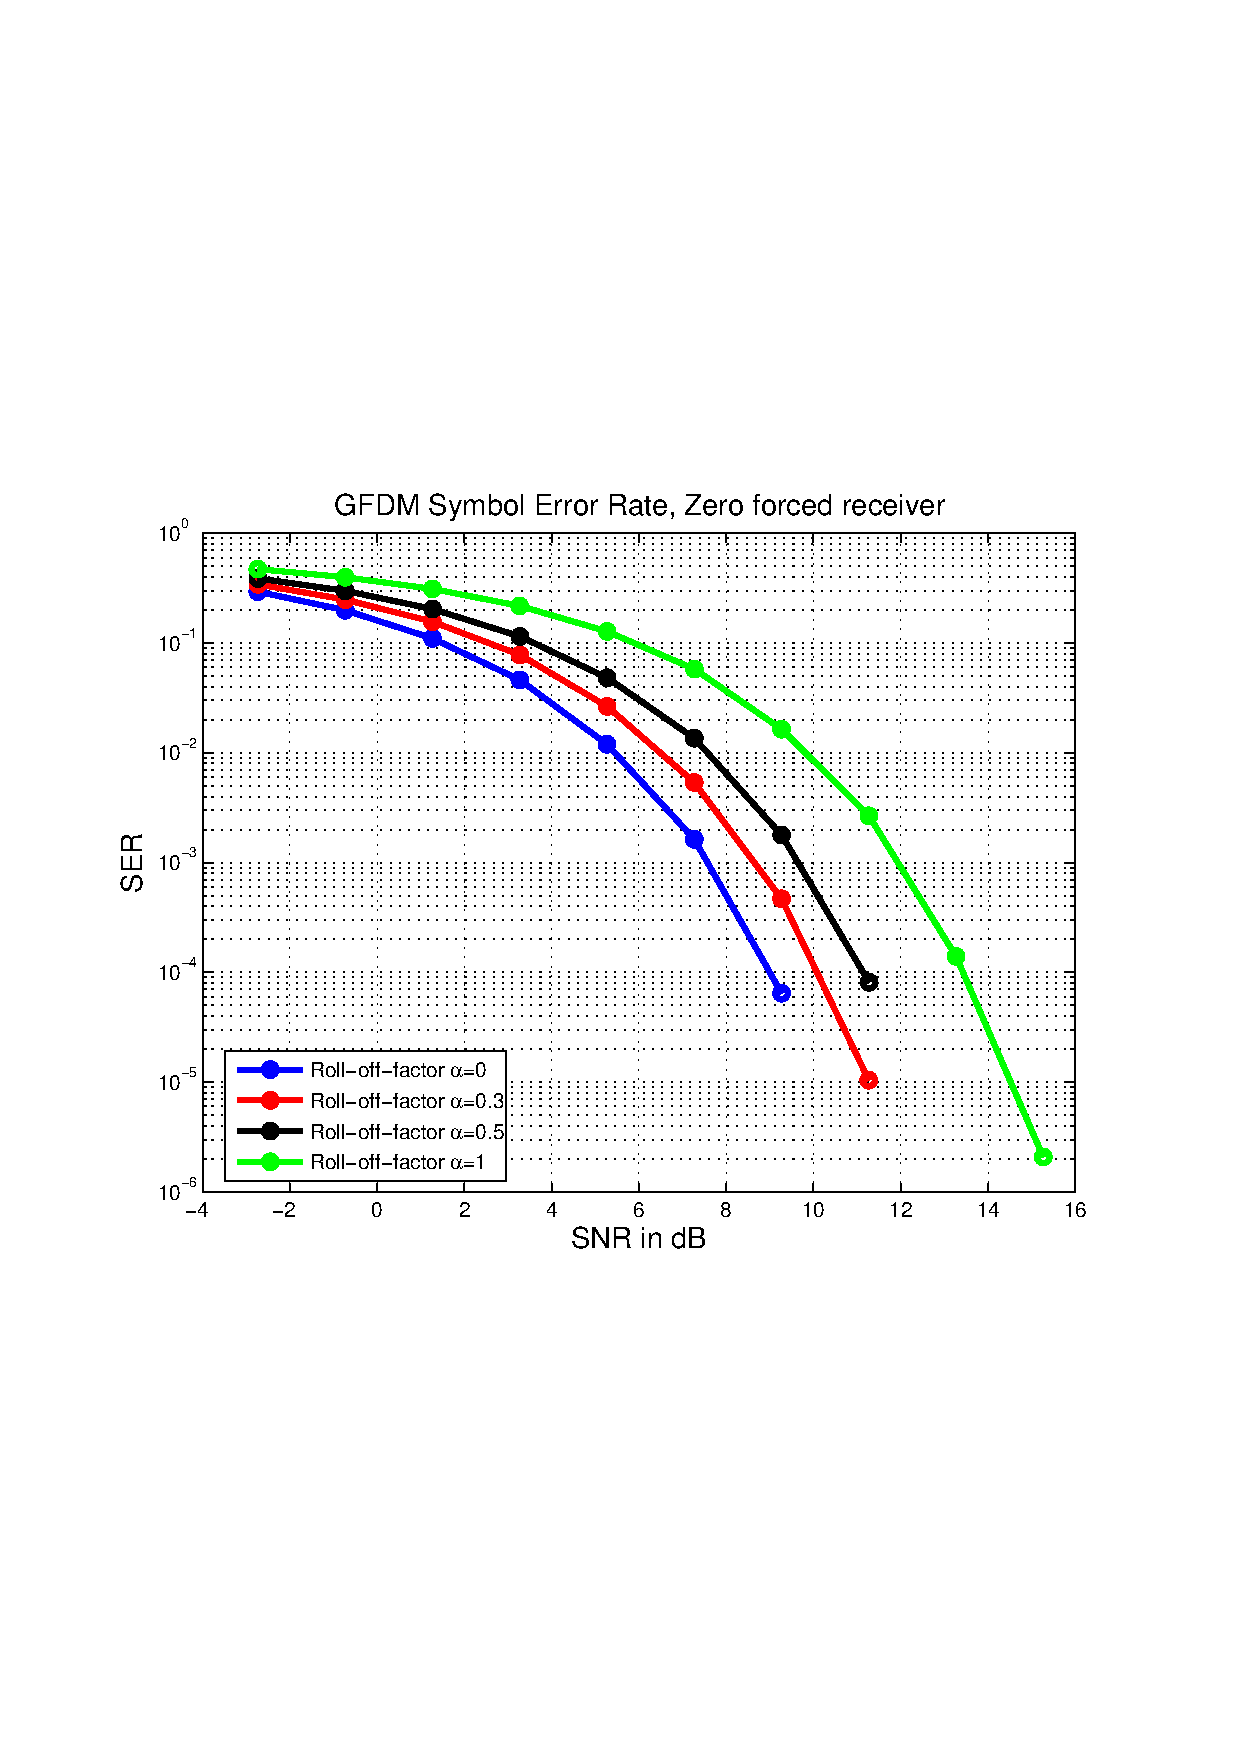
\includegraphics[width=0.9\columnwidth]{ZF_SER.png}
\caption{\textit{Зависимость производительности приемника от коэф. перекрытия $\alpha$ для приемника на псевдообратной матрице}}
\label{fs_1}
\end{figure}

\begin{figure}[H]
\centering
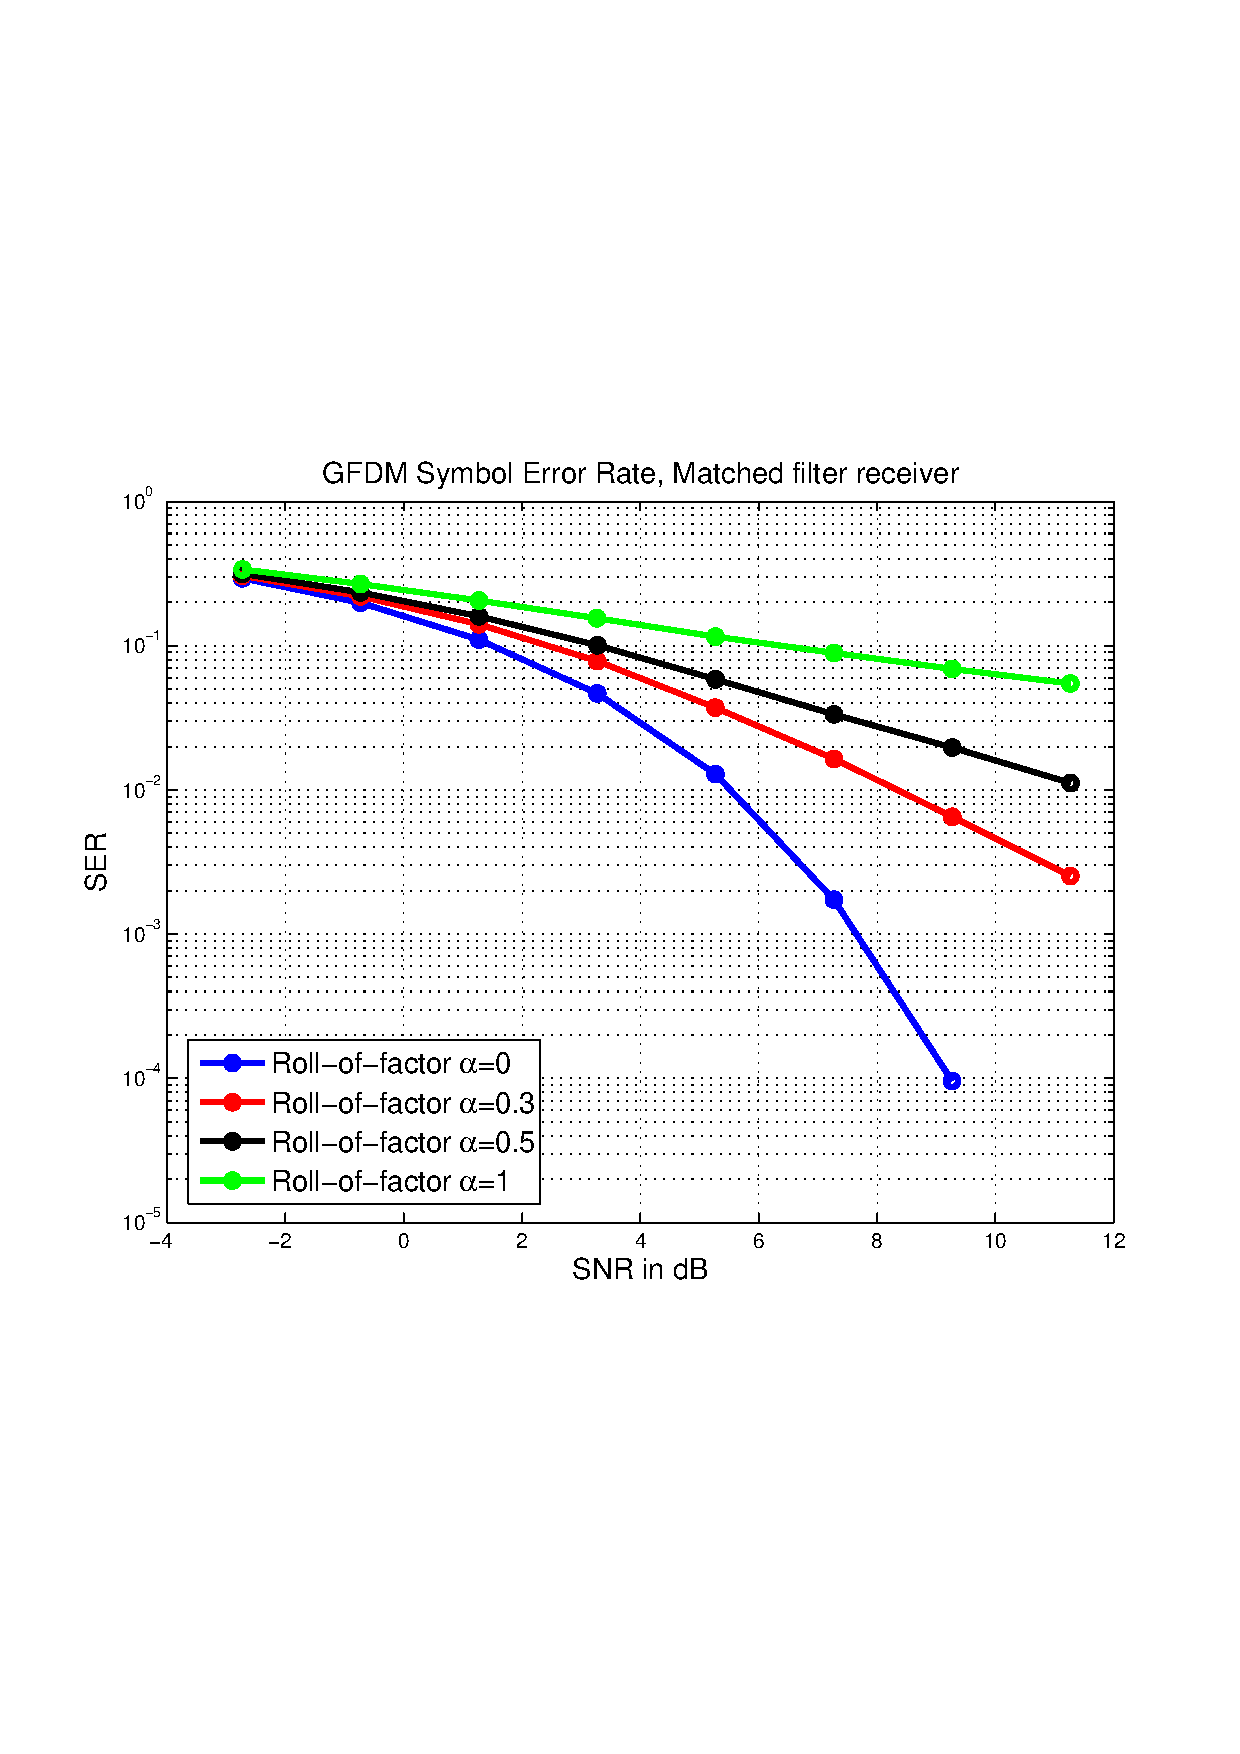
\includegraphics[width=0.9\columnwidth]{MF_SER.png}
\caption{\textit{Зависимость производительности приемника от коэф. перекрытия $\alpha$ для согласованного приемника}}
\label{fs_2}
\end{figure}
Производительность системы ОбЧРК для работы полу-слепого приемника получены при помощи моделирования. В системе был положен аддитивный белый Гауссов шум без какого либо кодирования. В системе была использована квадратурная фазовая манипуляция. Количество поднесущих равно $F=32$. Количество временных отсчетов на каждый временной символ равно $T/T_s=F$. Количество временных символов равно $T_s=15$. В качестве фильтра был использован фильтр с характеристикой "Корень из приподнятого косинуса" с коэффициентом перекрытия $\alpha=0.5$. Коэффициенты передачи для различных поднесущих были выбраны как случайные целочисленные величины в диапазоне от $0$ до $1$. На приемнике величины оцениваются как пороговые устройства и приравниваются разрешенным величинам. Результаты производительности системы ОбЧРК  показаны на двух рисунках, на первом рисунке показано соотношение символов к ошибкам в случае если приемник знает истинную величину вектора $\mathbf{a}$, при помощи приемника на псевдообратной матрице, если приемник если не знает истинную величину вектора $\mathbf{a}$.Кроме того показаны результаты работы двух версий полу-слепых приемников. На втором рисунке представлена нормализованная ошибку между истинным значением вектора истинную величину вектора $\mathbf{a}$ и найденным приемником.
\begin{table}[H]
\caption{\label{tab:sim_alpha}ОбЧРК эксперимент 1.2}
\begin{center}
\begin{tabular}{|c|c|c|}
\hline
Параметр & Обозначение & Значение \\
\hline
\hline
Вид модуляции & $\mu$ & КФМ-2 \\
\hline
Отсчетов на символ & $T/T_s$ & 32 \\
\hline
Поднесущие&$F$&32 \\
\hline
Разме блока передачи& $T_s$  &15 \\
\hline
Вид фильтра&  &КиПК \\
\hline
Коэффициент перекрытия&$\alpha$  &0.5 \\
\hline
Коэффициенты поднесущих& $\mathbf{a}_i$ & $randi([0 1])$ \\
\hline
Канал& $h$ &АБГШ \\
\hline
Префикс&  & Нет \\
\hline
Передача&  & Некодированно\\
\hline
\end{tabular}
\end{center}
\end{table}
\begin{figure}[H]
\centering
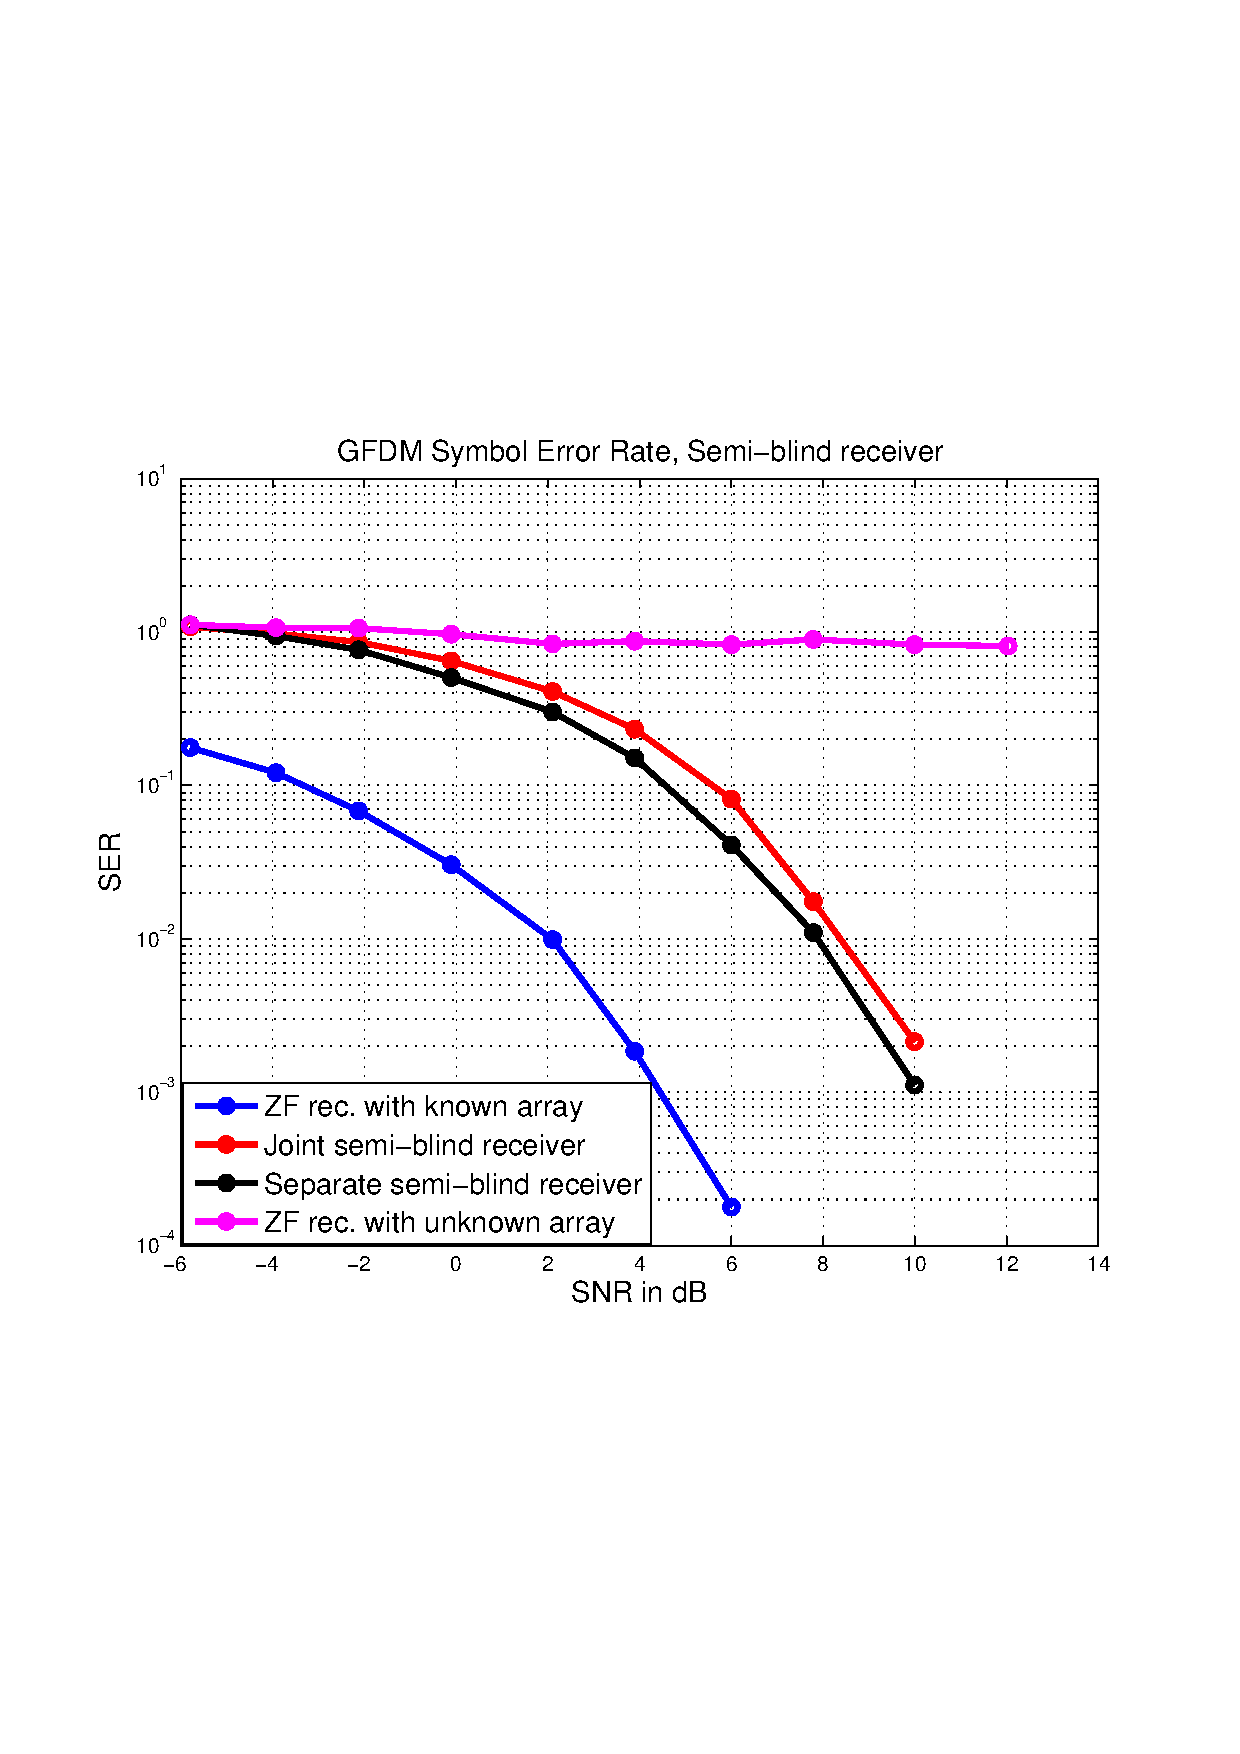
\includegraphics[width=0.9\columnwidth]{SM_SER.png}
\caption{\textit{Сравнение производительности для алгоритма поиска поднесущих}}
\label{fs_3}
\end{figure}
\begin{figure}[H]
\centering
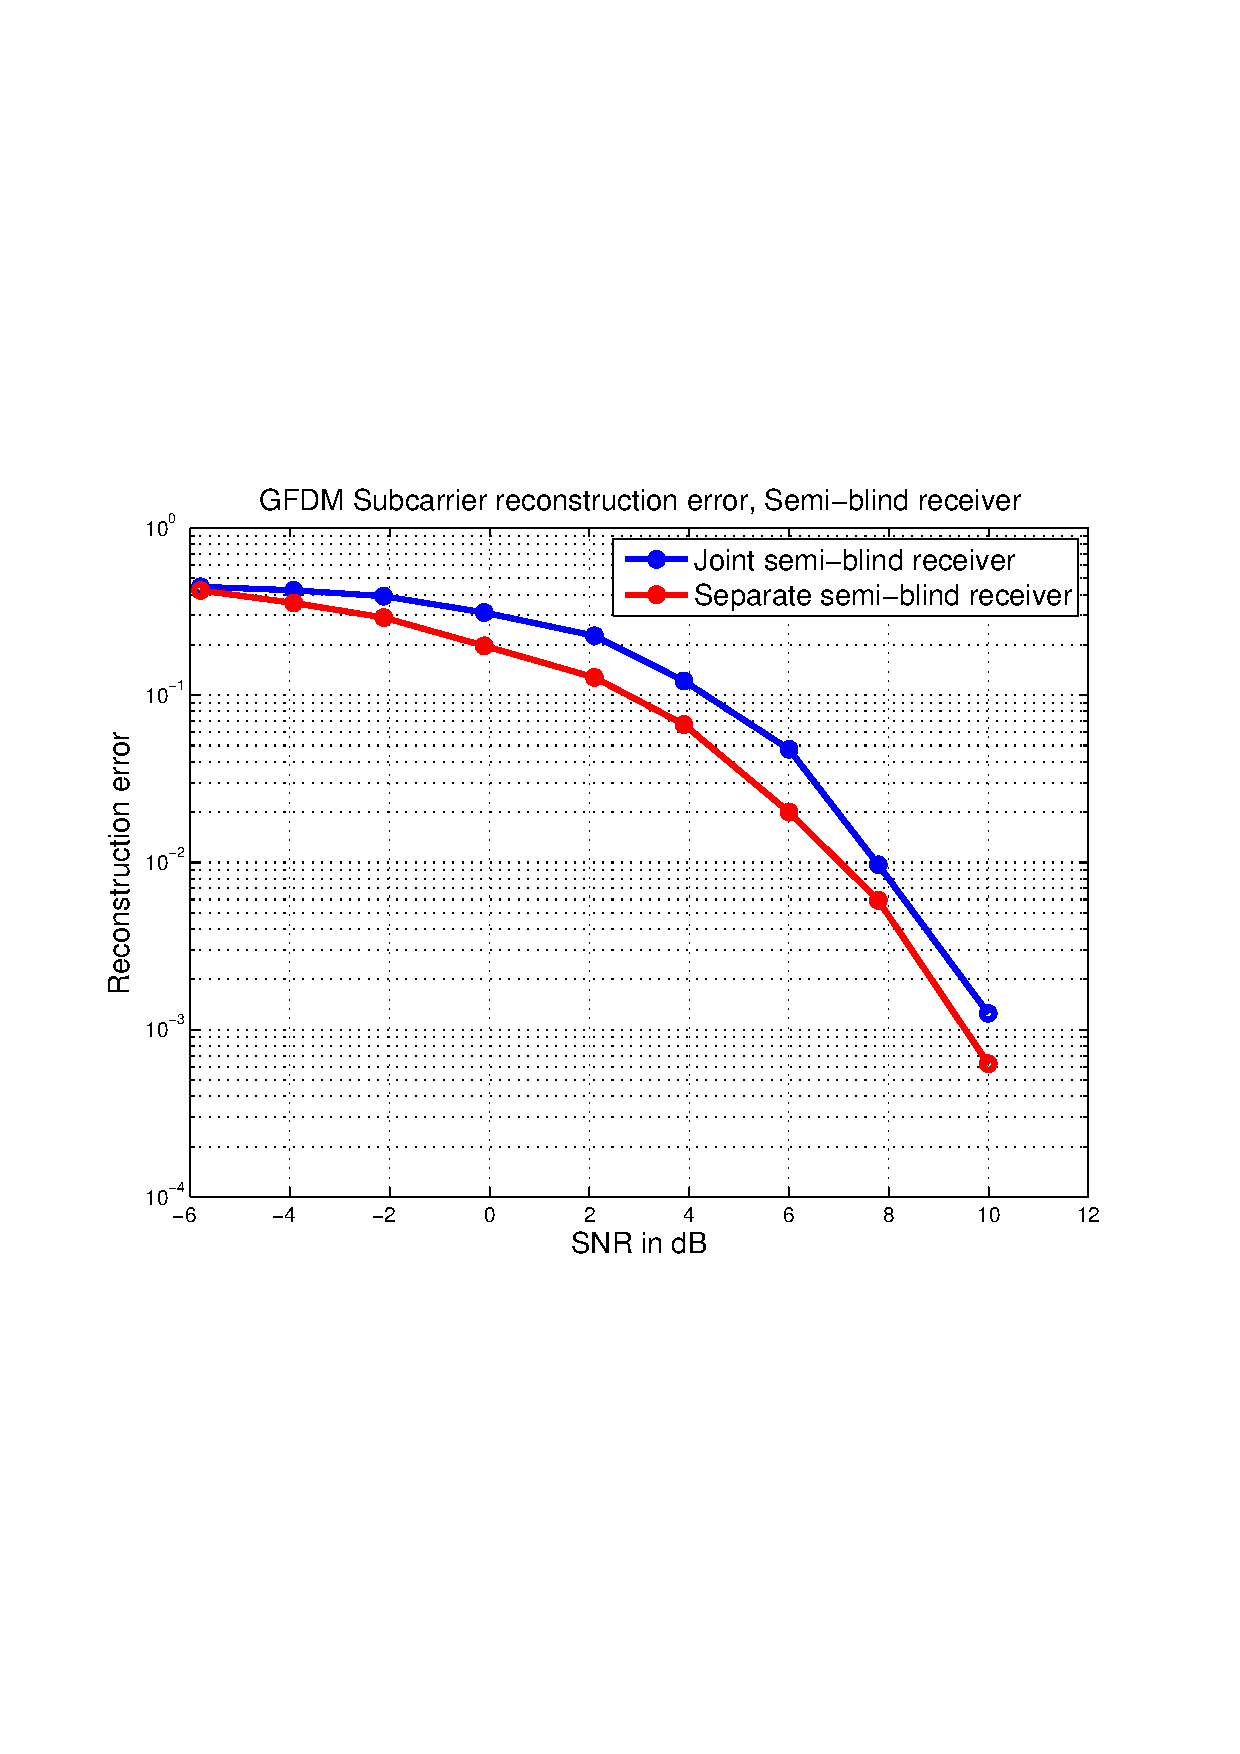
\includegraphics[width=0.9\columnwidth]{SM_RE.png}
\caption{\textit{Ошибка восстановления поднесущих}}
\label{fs_4}
\end{figure}
Кроме того мы добавили дополнительные графики для сравнения совместного и раздельного решения работы алгоритмов. Результаты сравнения так же получены при помощи моделирования.
\begin{table}[H]
\caption{\label{tab:sim_alpha}ОбЧРК эксперимент 1.3}
\begin{center}
\begin{tabular}{|c|c|c|}
\hline
Параметр & Обозначение & Значение \\
\hline
\hline
Сигнал/Шум & $log(P_s/P_n)$ & 10 \\
\hline
Отсчетов на символ & $T/T_s$ & 32 \\
\hline
Поднесущих&$F$&32 \\
\hline
Размер блока& $T_s$  &15 \\
\hline
Вид фильтра&  &КиПК \\
\hline
Коэффициент перекрытия&$\alpha$  &0.5 \\
\hline
Коэффициенты поднесущих& $randi([0 1])$ \\
\hline
\end{tabular}
\end{center}
\end{table}
\begin{figure}[H]
\centering
\includegraphics[width=0.9\columnwidth]{SM_conv.png}
\caption{\textit{Сходимость алгоритма по функции невязки}}
\label{fs_5}
\end{figure}
\begin{figure}[H]
\centering
\includegraphics[width=0.9\columnwidth]{SM_TIME.png}
\caption{\textit{Время сходимости алгоритма в зависимости от соотношения сигнал/шум}}
\label{fs_6}
\end{figure}
\begin{figure}[H]
\centering
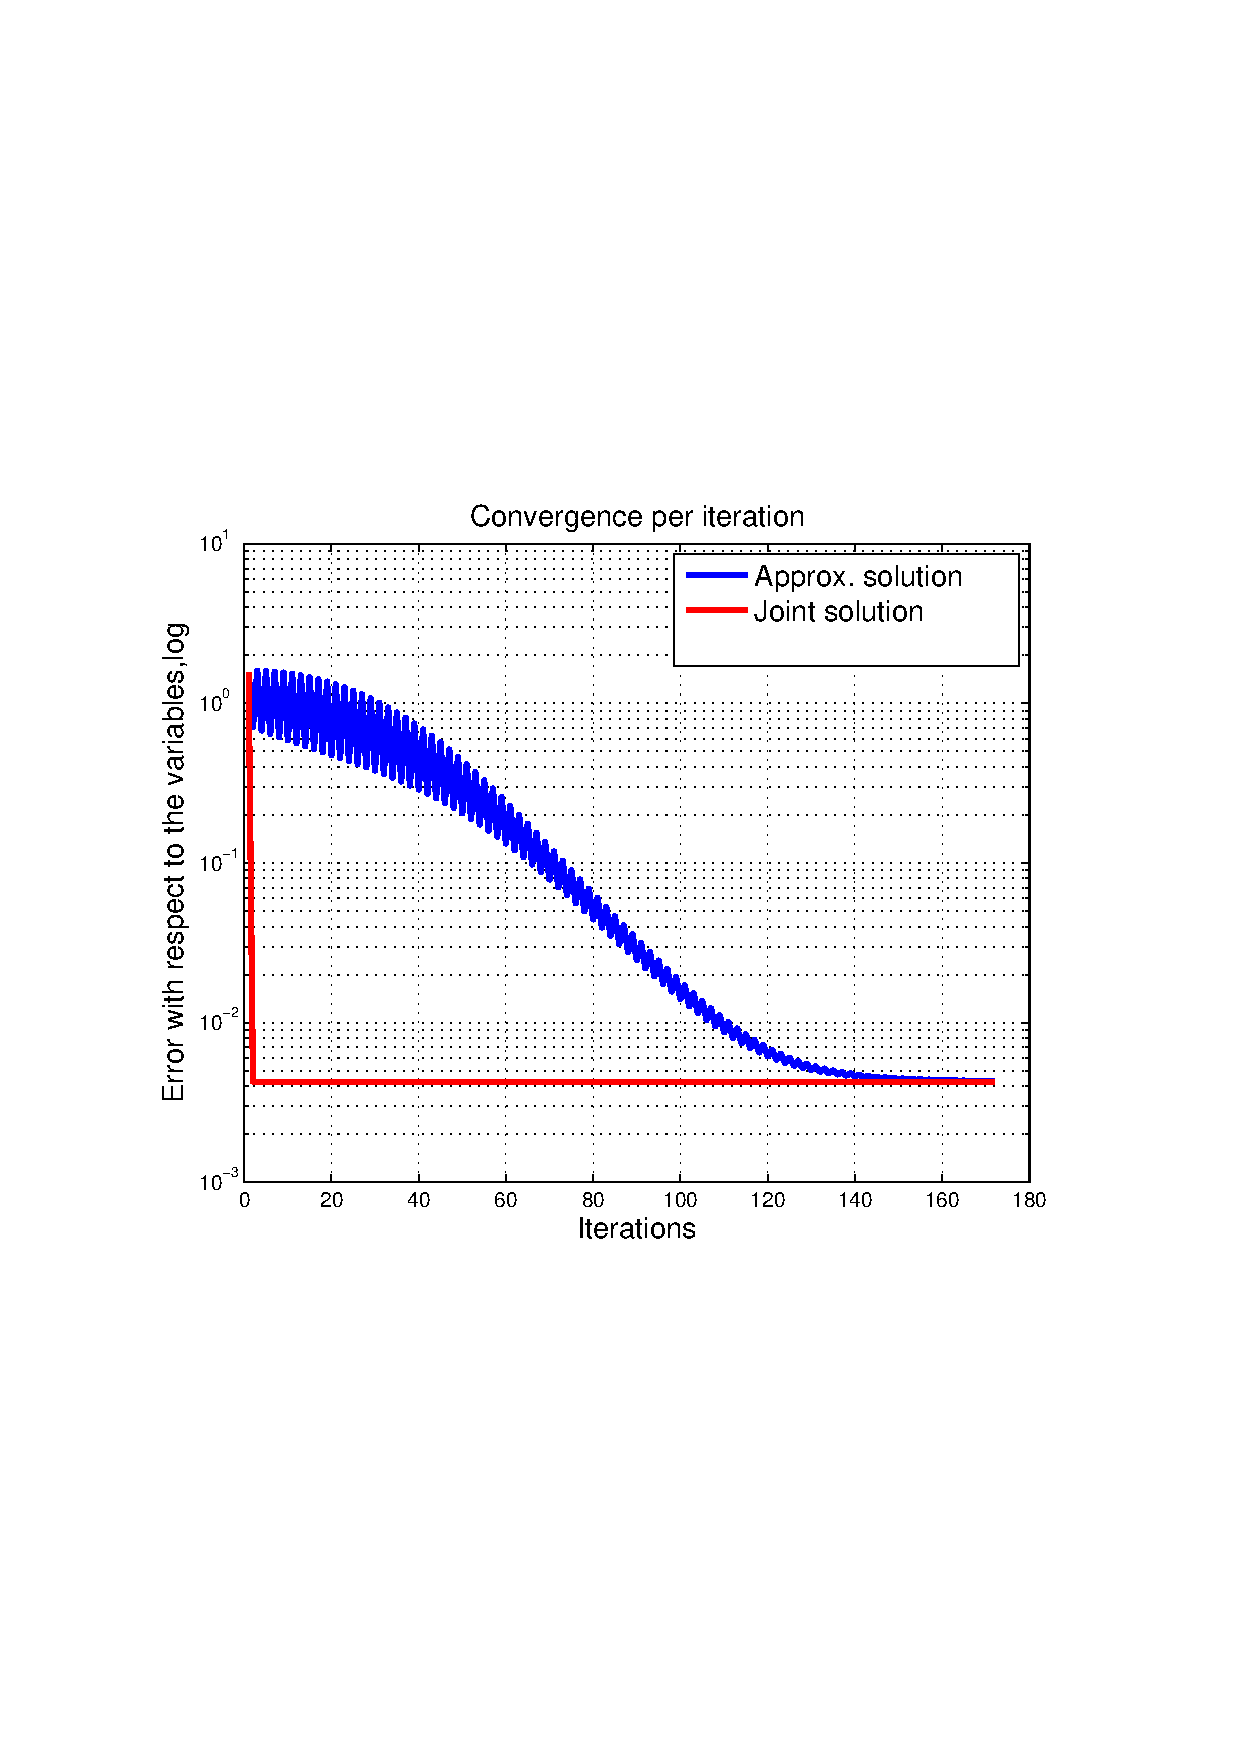
\includegraphics[width=0.9\columnwidth]{SM_RES.png}
\caption{\textit{Сходимость алгоритма по переменным}}
\label{fs_7}
\end{figure}
Производительность системы ОбЧРК для работы полу-слепого приемника получены при помощи моделирования. В системе был положен канал с памятью с дополнительным аддитивным белым Гауссовым шумом на входе приемника без какого либо кодирования. В системе была использована квадратурная фазовая манипуляция. Количество поднесущих равно $F=32$. Количество временных отсчетов на каждый временной символ равно $T/T_s=F$. Количество временных символов равно $T_s=32$. В качестве фильтра был использован фильтр с характеристикой "Корень из приподнятого косинуса" с коэффициентом перекрытия $\alpha=1$.  Результаты производительности системы ОбЧРК  показаны на двух рисунках, на первом рисунке показано соотношение символов к ошибкам для различного количества тренировочных символов и сравнение с приемником на обратной фильтрации. На втором рисунке представлена ошибка восстановления канала для различного количества тренировочных символов.

\begin{table}[H]
\caption{\label{tab:sim_alpha}ОбЧРК эксперимент 1.4}
\begin{center}
\begin{tabular}{|c|c|c|}
\hline
Параметр & Обозначение & Значение \\
\hline
\hline
Отсчетов на символ & $T/T_s$ & 32 \\
\hline
Поднесущих&$F$&32 \\
\hline
Размер блока& $T_s$  &15 \\
\hline
Вид фильтра&  &КиПК \\
\hline
Коэффициент перекрытия&$\alpha$  &1 \\
\hline
Тип канала& $Ped-A$ \\
\hline
\end{tabular}
\end{center}
\end{table}
\begin{figure}[H]
\centering
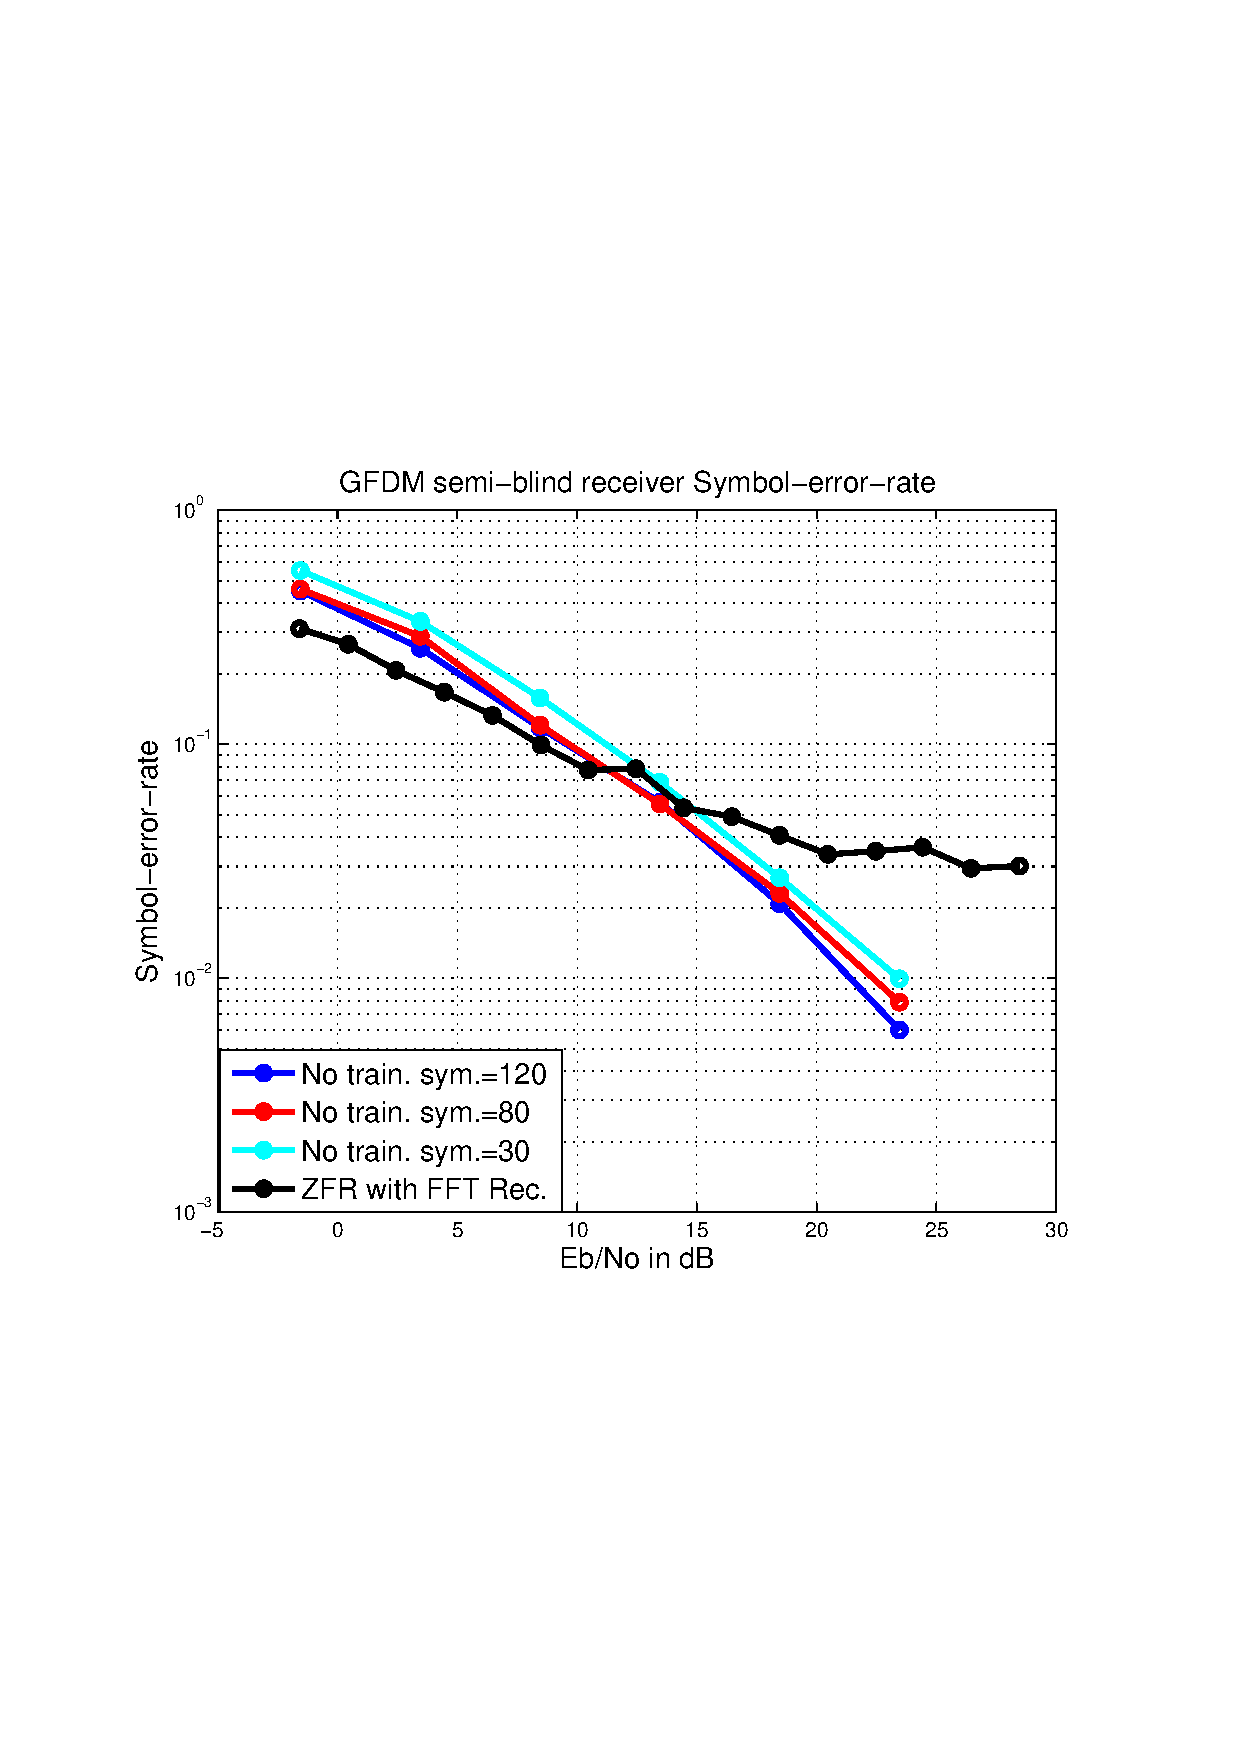
\includegraphics[width=0.9\columnwidth]{SM_SISO_FS_SER.png}
\caption{\textit{Производительность работы полу-слепого приемника от сигнал/шум и количества тренировочных символов}}
\label{fs_8}
\end{figure}
\begin{figure}[H]
\centering
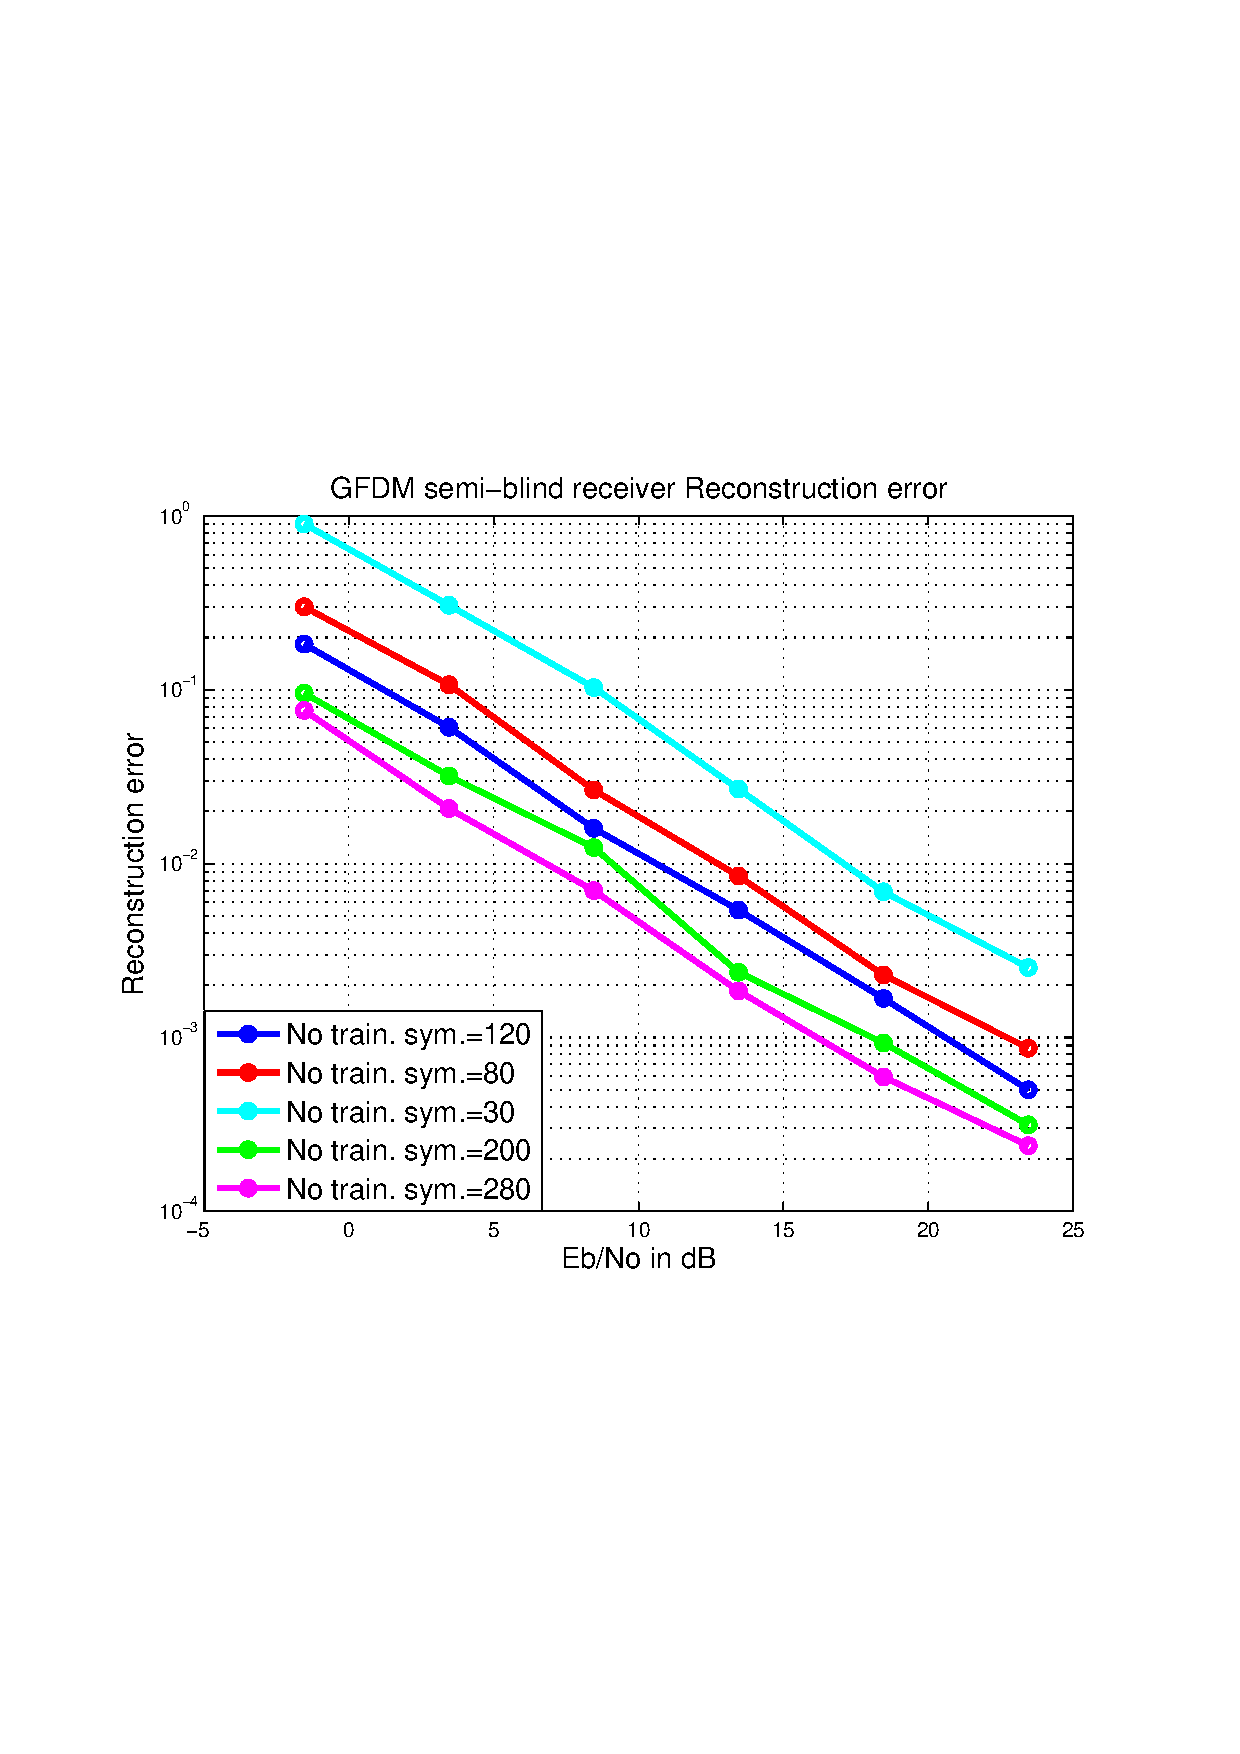
\includegraphics[width=0.9\columnwidth]{SM_SISO_FS_RE.png}
\caption{\textit{Ошибка восстановления канала полу-слепого приемника от сигнал/шум и количества тренировочных символов}}
\label{fs_9}
\end{figure}
\section{Заключение}
В качестве заключение по первому эксперименту мы можем сказать, что приемник на основе псевдообратной матрицы показывает значительно лучшие результаты в детектировании символов по сравнению с согласованными приемником. Разница между приемниками незначительная в случае если коэффициент перекрытия имеет малое значение. Однако увеличение коэффициента перекрытия значительно уменьшает производительность системы на основе согласованного фильтра. Это связано с тем, что увеличивается перекрытие по частоте $\alpha$ между поднесущими. Таким образом из рис.\ref{fs_1} видно что увеличение коэффициента перекрытия до максимума уменьшает производительность системы на 5 дБ. При этом производительность системы на основе согласованного фильтра значительно ухудшается, что видно на рис.\ref{fs_2} и делает применение согласованного фильтра бесполезным. Таким образом результаты показывают, что предпочтительнее использовать приемник на основе псевдо-обратной матрицы. Таким образом можно обеспечить лучшие результаты по вне-полосным излучениям системы при этом устранять влияние взаимной интерференции в системе. Более того можно использовать дополнительные алгоритмы для устранения взаимной интерференции в системе позволяющие получить дополнительное увеличение производительности.
В качестве заключения для эксперимента с анализом алгоритма оценки работающих подчастот можно сделать следующие выводы :
\begin{itemize}
\item Алгоритм позволяет определить была ли включена поднесущая и передавались ли по ней данные.
\item Использование алгоритма приводит к ухудшению производительности системы на 5-6дБ.
\item Алгоритм может быть доработан использованием дополнительных техник по принятию решения о том, была ли включена поднесущая.
\end{itemize}
Как сказано в п.1 алгоритм работает и позволяет автоматически, без вероятностных моделей определить были ли переданы данные по поднесущей, при условии что для приемника известен хотя бы один символ на каждой из поднесущих. Однако применение системы при сравнении со случаем, когда приемник идеально знает используемые поднесущие приводит к ухудшению производительности на 5 дБ что показано на рис.\ref{fs_3}. Данное снижение в производительности связано с тем, что увеличивается количество источников ошибок, и в случае если приемник ошибочно определил поднесущую как включенную, это приводит к большому количеству ошибок. При этом цена ошибки принятия решения оказывается высокой, в то время как в функцию невязки оба выражения входят с одинаковым коэффициентом. В качестве решающего устройства было использовано пороговое устройство оценивавшее абсолютную величину коэффициента поднесущей, в случае если величина была больше 0.5 поднесущая считалась включенной. Поскольку данное решение не является оптимальным, возможно применение иных техник для увеличения эффективности алгоритма. Кроме того как показывают результаты на рис.\ref{fs_3}и рис.\ref{fs_4} , приближенный алгоритм имеет производительность лучше, чем у алгоритма с полной точностью. Это может быть связано с тем, что приближенное решение  имеет тенденцию к ошибкам типа "пропуск сигнала", и поскольку было оценено меньшее количество поднесущих чем на самом деле было использовано, то и количество соответствующих ошибок окажется меньше. Таким образом с точки зрения данной метрики производительность является большей, однако она является несущественной. Так же дополнительные рисунки показывают преимущества алгоритма с полной точностью. Как видно из рис.\ref{fs_5}. Скорость сходимости алгоритмов отличается значительно. Алгоритм полной точности сходится всего за две итерации, что позволяет уменьшить количество вычислений во много раз, в то время как алгоритм  приближенной точности требует в среднем 100-200 итераций для сходимости. Таким образом последующая зависимость времени сходимости алгоритма на рис. \ref{fs_6} оказывается значительно лучше у алгоритма полной точности из-за количества итераций приближенного алгоритма. При этом даже, тот факт, что каждая итерация алгоритма приближенной точности требует меньше вычислительных ресурсов, в итоге алгоритм затрачивает значительно больше  ресурсов. Как можно видеть из рис. \ref{fs_7} сходимость алгоритма приближенной точности происходит нелинейно и достаточно нестабильно, вызывая колебания ошибки восстановления на каждой итерации. Это вызывает долгий итерационный процесс, что и является следствием столь долгой сходимости алгоритма.

Эксперимент по проверке работы полу слепого приемника оценивающего состояние канала и принятые символы показывает следующие результаты:
\begin{itemize}
\item Правильным образом выбирая известные символы в блоке данных можно достичь даже лучшей производительности, чем если идеально знать канал и делать поиск по всем возможным символам.
\item Алгоритм показывает хорошую производительность по каналу пешеходного типа А. 
\item Производительность алгоритма зависит от количества неизвестных символов.
\end{itemize}
Как видно из рис. производительность системы  полу-слепым приемником на основе оптимизации показывает результат лучше, чем даже если был бы использован приемник на основе обратной фильтрации с идеально известным каналом, что говорит о больше стабильности алгоритма. Однако подобное поведение будет изменяться в случае если будут включены только некоторые поднесущие. Производительность системы меняется в зависимости от того сколько символов в блоке данных известно для приемника. После некоторой величины производительность системы падает ниже уровня приемника с идеально известным каналом. Таким образом можно адаптивно регулировать производительность системы. Как видно из рис. кривые ошибки восстановления канала лежат параллельно друг другу позволяя так же адаптивно выбирать точность определения канала гибко, таким образом обновляя состояние канала если он не меняется и уменьшать количество символов на первой итерации для более точного определения канала. Кроме того благодаря использованному подходу с вычитанием известных символов из функции невязки взаимная интерференция между разными каналами так же уменьшается и дополнительно увеличивает производительность системы. Кроме того в случае постановки задачи оптимизации количества излучаемой энергии к количеству полученной информации будет получена вогнутая кривая производительности по качеству работы системы в зависимости от количества известным системе символов.
Основным выводом можно считать что данный подход является чрезвычайно эффективным с точки зрения качества работы системы, однако не является реализуемым на практике с точки зрения оборудования, так как потребует значительных вычислительных ресурсов, однако возможна параллельная обработка принятых данных, что вероятно может ускорить работу системы. Более того для простых задач с небольшими объемами данных современные встроенные системы могут реализовать данные операции.
\clearpage

\chapter{Обобщенное частотное разделение каналов в системе с количеством антенн больше двух}
\section{Модель системы}
В данном разделе мы рассматриваем ОбЧРК МВМВ систему в канале без памяти с Рэлеевским замиранием\cite{Book25}\cite{Book29}. Система может быть описана при помощи выражения \eqref{mim_1} включая в себя канальную и шумовую составляющую в модель. Данная модель не рассматривает многолучевое распространение в среде передачи.
\begin{align}
\mathbf{Y}=\mathbf{HX}+\mathbf{N}
\label{mim_1}
\end{align}
\begin{align*}
\mathbf{H}\in\compl^{M_r\times M_t}
\mathbf{X}\in\compl^{M_t\times T}
\mathbf{N,Y}\in\compl^{M_r\times T}
\end{align*}
 Система ОбЧРК в случае МВМВ так же может быть рассмотрена как модель $PARATUCK2$ третьего порядка. Разница между ОВОВ и МВМВ модели значительна\cite{Book29}, поэтому для использования аналогичной тензорной модели необходимо изменить одну из генерирующих матриц модели, а так же метод формирования двух других. Однако в результате можно описать МВМВ модель при помощи той же тензорной алгебры. Размерность принятых данных равна произведению количества принимающих антенн на размер блока данных.
Матрица символов должна быть составлена из тензора третьего порядка размерности $\mathcal{S}\in \compl^{F\times T_s\times M_t}$ в случае МВМВ модели. Дополнительная размерность связана с тем, что каждая передающая антенна передает свой собственный набор символов не равный с другими антеннами. Однако модель $PARATUCK2$ не предусматривает использование тензоров в модели. Для того чтобы преодолеть данное ограничение тензор $\mathcal{S}$ был переписан как соединенные во второй размерности друг с другом слои по третьей размерности. Выражение можно переписать следующим образом \eqref{mimo_1}. Иначе говоря так же можно сказать что матрица $\mathbf{S}$ равна развертке тензора $\mathcal{S}$ по второй размерности с транспонирование.
\begin{align}
\mathbf{S}=\begin{bmatrix}
\mathcal{S}_{:,:,1}\\
\mathcal{S}_{:,:,2}\\
\vdots \\
\mathcal{S}_{:,:,M_t}\\
\end{bmatrix} \label{mimo_1}
\end{align}
\begin{align*}
\mathcal{S}\in\compl^{F\times T_s\times M_t}
\mathbf{S}\in\compl^{F\cdot M_t\times T_s}
\end{align*}
Матрица$C^{[b]}$ при переходе из ОВОВ модели в МВМВ остается неизменной и не зависит от количества используемых антенн\eqref{mim_2}. В столбцах матрицы остаются фильтрующие последовательность для различных временных слотов которые не зависят от количества антенн. Таким образом правая часть выражения $\mathbf{S}$ не изменяется и имеет аналогичное количество столбцов $T_s$ как в модели ОВОВ.
\begin{align}
\mathbf{C}^{[b]}\in\compl^{T\times T_s}
\label{mim_2}
\end{align}
Вектор связи  $\mathbf{b}$ так же остается не подвергается изменениям при переходе в модель МВМВ \eqref{mimo_3}. Необходимо заметить, что это верно в случае если мы продолжаем рассматривать линейную независящую от времени в пределах передачи одного блока данных модель распространения сигнала. В таком случае вектор  $\mathbf{b}$ будет представлять собой вектор заполненный единичными значениями. 
\begin{align}
\mathbf{b}=\mathbf{1}_{T_s\times 1} \label{mimo_3}
\end{align}
\begin{align*}
\mathbf{b} \in\compl^{T_s\times 1} 
\end{align*}
Матрица $\mathbf{C}^{[a]}$ и $\mathbf{S}$ в случае модели МИМО должны быть изменены. Определим эту матрицу как $\mathbf{C}^{[a]'}$.Согласно размерностям матрицы $\mathbf{S}$, размерность матрицы  $\mathbf{C}^{[a]'}$ должна быть $\mathbf{C}^{[a]'} \in \compl^{T\times F\cdot M_t}$. В сравнении с моделью ОВОВ, в случае МВМВ матрица С должна быть умножена так же с матрицами на основе $\mathbf{C}^{[a]}$. Таким образом матрица $\mathbf{C}^{[a]'}$ должна быть построена на повторении $M_t$ раз матрицы $\mathbf{C}^{[a]}$. Поскольку произведение Адамара представляет собой перенос на другую частоту для каждой из поднесущих модифицированная матрица $\mathbf{C}^{[a]'}$ станет модуляцией всех поднесущих поочередно на каждой из передающих антенн $m_t$. Поскольку все поднесущие на каждой из передающих антенн равны, то их можно собрать простым связыванием одной генерирующей матрицы.
\begin{align}
\mathbf{C}^{[a]'}=
\begin{bmatrix}
\mathbf{C}^{[a]}& \mathbf{C}^{[a]}& \cdots &\mathbf{C}^{[a]}\\
\end{bmatrix} \in\compl^{T\times M_t\cdot F} \label{mimo_4}
\end{align}
\begin{align}
\mathbf{C}^{[a]'}=(\mathbf{1}_{1\times M_t} \otimes \mathbf{C}^{[a]}) \in \compl^{  T\times M_t\cdot F} \label{mimo_5}
\end{align}
Вектор $\amat$ становится  матрицей $\Amat$ и соединяет каждую приемную антенну $m_t$ с каждой поднесущей каждой передающей антенны с коэффициентами передачи для каждой поднесущей.Определим данные коэффициенты в виде тензора $\mathcal{A}$\eqref{mimo_7} включающего коэффициенты для каждой приемной, передающей антенны и поднесущей $m_r,f,m_t$. В модели $PARATUCK2$ тензор $\mathcal{A}$ должен быть представлен в виде матрицы, который будет суммировать все коэффициенты поднесущих  для всех передающих антенн. Размерность матрицы $\Amat$ равна $\Amat \in \compl^{M_r\times F\cdot M_t}$. Таким образом развертка первого порядка тензора $\mathcal{A}$ удовлетворяет данному условию по размерностям\eqref{mimo_8}. 
\begin{align}
\mathcal{A} \in \compl^{M_r\times F\times M_t} \label{mimo_6}
\end{align}
\begin{align}
\mathbf{A}=\mathcal{A}_{[1]} \label{mimo_7}
\end{align}
\begin{align}
\mathbf{A}\in\compl^{M_r \times F\cdot M_t} \label{mimo_8}
\end{align}
Общая модель для МВМВ модели с представленными выше матрицами определена в выражении. Данная модель показывает принятые данные для принятого сигнала без учета влияния шума.Все операции описанные в случае ОВОВ так же могут быть описаны в случае с МВМВ с некоторыми расширениями. Следует заметить что ранг матрицы $\mathbf{A}$ равен $rank(\Amat)=min(M_r,F\cdot M_t)$  и в реальном случае значение в правой части оператора значительно меньше значения в левой его части. Ранг матрицы $\mathbf{A}$  показывает как много потоков передачи данных может открыть система между данным набором антенн. 
\begin{align}
\mathbf{HX}=\mathbf{A}\cdot (\mathbf{C}^{[a]'T} \odot (\mathbf{S}\cdot (\mathbf{C}^{[b]}\diamond \mathbf{B})^T)) \label{mimo_9}
\end{align}
\begin{align*}
\mathbf{HX}\in\compl^{M_r \times T}
\mathbf{A}\in\compl^{M_r \times F\cdot M_t}
\mathbf{C}^{[a]'}\in\compl^{T \times F\cdot M_t}
\end{align*}
\begin{align*}
\mathbf{S}\in\compl^{F\cdot M_t \times T_s}
\mathbf{C}^{[b]}\in\compl^{T \times T_s}
\mathbf{B}\in\compl^{1 \times T_s}
\end{align*}

\section{Ортогонализация влияния канала без частотной избирательности}
Приемник и передатчик совместно могут ортогонализировать влияние канала путем схожим со стандартной ортогонализацией в МВМВ системах. Очевидно подход имеет дополнительные изменения если мы полагаем модель канала равную матрице $\mathbf{A}$. Это связано с тем что ранг матрицы $\mathbf{A}$ значительно меньше количества возможных для ортогонализации потоков. В стандартном подходе для ортогонализации два шага: предобработка и постобработка. Канальная матрица $\mathbf{A}$ может быть разложения при помощи сингулярного разложения матрицы на три матрицы компоненты $\mathbf{U \Sigma V}$.
\begin{align}
\mathbf{A}=\mathbf{U}\cdot \mathbf{\Sigma} \cdot \mathbf{V}^H \label{mimo_co_1}
\end{align}
\begin{align*}
\mathbf{A} \in\compl^{M_r \times F\cdot M_t}
\mathbf{U} \in\compl^{M_r \times M_r }
\mathbf{\Sigma} \in\compl^{M_r \times F\cdot M_t }
\mathbf{V} \in\compl^{F\cdot M_t \times F\cdot M_t }
\end{align*}
\begin{align}
\mathbf{A}=\mathbf{U}_e\cdot \mathbf{\Sigma}_e \cdot \mathbf{V}_e^H \label{mimo_co_2}
\end{align}
\begin{align*}
\mathbf{A} \in\compl^{M_r \times F\cdot M_t}
\mathbf{U} \in\compl^{M_r \times r }
\mathbf{\Sigma} \in\compl^{r \times r }
\mathbf{V} \in\compl^{F\cdot M_t \times r }
\end{align*}
 Передатчик для ортогонализации умножает слева передаваемые данные на матрицу $\mathbf{V}$ которая является матрицей обратной к $\mathbf{V}$. Приемник так же умножает принятые данные на матрицу обратную к матрице $\mathbf{U}$. 
Матрица $\mathbf{\Sigma}$ имеет диагональную структуру и не смешивает данные, однако взвешивает на  коэффициенты. Следует заметить что невозможна диагонализация этим путем количества каналов больше чем ранг матрицы $\mathbf{A}$. Однако как было записано ранее истинное количество потоков данных значительно больше чем ранг $\mathbf{A}$. Стандартный метод не использует ортогональность поднесущих частот и разрушает ортогональную структуру матрицы $\Camat$. Однако структура матрицы $\Camat$ может быть использована для того чтобы ортогонализировать потоки данных соответствующие различным поднесущим у одной и той же передающей антенны. Таким образом строкам в матрице $\mathbf{S}$ могут соответствовать ортогональные из-за различных поднесущих потоки. 
Передатчик обеспечивает предобработку и изменяет матрицу $\Camat$ таким образом чтобы ортогонализировать максимальное количество строк в матрице $\Amat$. Диагонализация в одно частотной МВМВ системе является произведением с матрицей $\mathbf{V}$ из сингулярного разложения матрицы $\mathbf{A}$. Однако а данном случае матрица предобработки будет построена на основе матрицы $\mathbf{V}$ однако будет от нее отличаться. Матрица отрогонализации строится таким образом чтобы тот же базис столбцов соответствовал различным поднесущим одной и той же передающей антенны. Матрица $\mathbf{A}$ состоит из блоков коэффициентов для соответствующей передающей антенны  но разным поднесущим частотам. Согласно ортогональности для различных поднесущих мы можем использовать для тот же самый базис матрицы $\mathbf{V}$. Таким образом приемник получает $r$ параллельных потоков от $M_t$ передающих антенн. Первый блок $M_t$ результирующей $\mathbf{V}_1$ матрицы состоит из повторения одного и того же столбца матрицы $\mathbf{V}$.
\begin{align}
r=rank(\mathbf{A})\label{mimo_co_3}
\end{align}
\begin{align}
\mathbf{V}_1=\begin{bmatrix}\mathbf{V}^{(1)} & \mathbf{V}^{(2)} & \cdots & \mathbf{V}^{(f)} &\cdots&\mathbf{0}^{(r+1)}&\cdots &\mathbf{0}^{(M_t)}\\
\end{bmatrix} \label{mimo_co_4}
\end{align}
\begin{align*}
\mathbf{V}_1\in \compl^{F\cdot M_t \times F\cdot M_t}
\end{align*}
\begin{align}
\mathbf{V}^{(k)}=\begin{bmatrix}
\mathbf{V}_{1,:}^{\mathbf{1}}&\mathbf{V}_{k,:}^{\mathbf{2}}&\cdots &\mathbf{V}_{k,:}^{\mathbf{F}}\\
\end{bmatrix} \in \compl^{F\cdot M_t \times F}
\end{align}
%\begin{align}
%\mathbf{\Sigma}\cdot \mathbf{V}^H \cdot \mathbf{V}_1=[\mathbf{\Sigma}^{(1)}_{1:M_t},\mathbf{\Sigma}^{(2)}_{1:M_t}\cdots \mathbf{\Sigma}^{(F)}_{1:M_t}] \label{mimo_co_5}
%\end{align}
\begin{align}
\mathbf{\Sigma}\cdot \mathbf{V}^H \cdot \mathbf{V}_1=\mathbf{\Sigma}_{1:M_t}\otimes \mathbf{1}_{1\times F} \label{mimo_co_5}
\end{align}
Процесс пост обработки остается аналогичным с классической МВМВ системой. Таким образом пред-обработка и пост-обработка позволяет трансформировать влияние матрицы канала на взвешивание каждого потока данных на какую либо величину при помощи матриц специальной структуры. При этом первые $M_t$ сингулярные значения матрицы $\mathbf{\Sigma}$ умножаются произведение Кронекера с вектором строкой состоящим из единиц. Количество возможных потоков будет зависеть от ранга матрицы $\mathbf{A}$ однако будет сохранять ортогональную структуру матрицы $\Camat$ и увеличивать количество потоков на количество поднесущих.  Общее количество потоков будет равно $rF$. Следует заметить произведение с матрицей обратной с $\mathbf{\Sigma}$ позволит нормализовать потоки данных к одному множителю. Матрица $\mathbf{\Upsilon}$ записана со структурой основанной на произведение Кронекера. Описанная операция позволяет ортогонализировать влияние канала внутри модели $PARATUCK2$. Для ортогонализации передатчик должен лишь домножить с левой стороны передаваемый вектор на сконструированную описанным образом матрицу. Для приемника ортогонализация не будет отличаться от процесса описанного для классической МВМВ ортогонализации.

\begin{align}
\mathbf{\Upsilon}=\mathbf{\Sigma}_e^{-1}\cdot \mathbf{U}^H\cdot \mathbf{U}\mathbf{\Sigma}\cdot \mathbf{V}^H \cdot \mathbf{V}_1=\begin{bmatrix}
\mathbf{1}_{1\times r} \otimes \mathbf{I}_{F}&\mathbf{1}_{1\times (M_t-r)} \otimes \mathbf{0}_{F}\\
\end{bmatrix} \label{mimo_co_6}
\end{align}
\begin{align}
\mathbf{X}=\mathbf{A}\cdot \mathbf{V}_1 (\mathbf{C}^{[a]T} \odot (\mathbf{S}\cdot (\mathbf{C}^{[b]}\diamond \mathbf{B})^T)) \label{mimo_co_8}
\end{align}
\begin{align}
\mathbf{A}^{[o]}=\mathbf{A}\cdot\mathbf{V}_1 \label{mimo_co_9}
\end{align}
\begin{align*}
\mathbf{V}_1 \in\compl^{M_t\cdot F \times M_t\cdot F}
\mathbf{\Delta} \in\compl^{M_r \times M_t\cdot F}
\mathbf{A}^{[o]} \in\compl^{M_r \times M_t\cdot F}
\end{align*}
\section{Поиск коэффициентов передачи поднесущих}
Использование алгоритмов спектрального сканирования так же применимо и в случае с МВМВ моделью. Одно из важных свойств модели МВМВ является разнесенность или свободность зачастую достигаемая при помощи пространственного положения антенн\cite{Book29}. Важно заметить что для различных пар приемник-передатчик может быть занята какая либо поднесущая другой системой. Приемник должен знать матрицу $\mathbf{A}$ для того чтобы знать каким образом были переданы данные. В случае неизвестности для приемника коэффициентов передачи поднесущих задача становится значительно сложнее в силу смешивания данных как во временной так и частотной области. Количество неизвестных для переменных для приемника в таком случае равно $ M_r M_t F$. Количество выражений которые считывает приемник равно для каждого блока данных $TM_r$. Как видно количество неизвестных может быть значительно больше количества известных величин. Однако приемник может найти данные коэффициенты при помощи специальным образом структурированной матрицы символов.
\subsection{Метод поиска основанный на ОВОВ модели}
Одним из способов для поиска матрицы $\mathbf{A}$ является полу-слепой приемник основанный на модели ОВОВ. Приемник может использовать алгоритм описанный в предыдущей части. Передатчик должен сконструировать символы для передачи специальным образом в матрице $\mathbf{S}$ и приемник должен знать как минимум ФМТ символов для поиска всех коэффициентов. Передатчик должен передавать данные как минимум $M_t$ временных слотов с известными символами для того чтобы найти матрицу $\mathbf{A}$. Алгоритм для поиска матрицы $\mathbf{A}$ следующий.
\begin{itemize}
\item Передатчик располагает внутри блока данных специально структурированные символы. Передатчик кладет известные приемнику символы в одну строку для искомой передающей антенны в каждую из поднесущих. Другими словами символы передаются только от определенной передающей антенны каждый временной слот. Передатчик повторяет процесс для каждой передающей антенны в последующие временные интервалы. Таким образом процесс занимает $M_t$ временных интервалов. При этом передатчик должен знать что и когда передавалось.
\item Приемник считывает на входе блок данных с длительностью $M_t$ временных интервалов. Приемник использует полу-слепой алгоритм для ОВОВ и полагает,что принятый сигнал передан от системы с моделью ОВОВ. Таким образом алгоритм позволяет найти значения коэффициентов поднесущих для первой передающей антенны.
\item Приемник повторяет данный процесс $M_t$ раз находя для каждого временного интервала свой блок коэффициентов для того чтобы найти все $M_tM_rF$ коэффициентов матрицы $\mathbf{A}$.
\end{itemize}
\subsection{Алгоритм основанный на МВМВ модели}
Матрица $\mathbf{A}$ может быть найдена при помощи следующего выражения  разделяющего в модели $PARATUCK2$ генерирующую матрицу и векторизированную матрицу $\mathbf{A}$\eqref{mimo_msm_5}. Модель может быть записана как произведение векторизированной матрицы $\mathbf{A}$ и матрицы промежуточной $\mathbf{\Delta}$ являющейся генератором. Данное произведение  может быть выражено с векторизацией для обеих матриц\eqref{mimo_msm_4}. Мы использовали данное свойство для того чтобы найти коэффициенты поднесущих матрицы $\mathbf{A}$ из принятых данных \eqref{mimo_msm_5}. Запишем функцию невязки минимум которой необходимо найти в квадратной норме. При этом выразим невязку относительно векторизированной матрицы $\mathbf{A}$\eqref{mimo_msm_6}. Поскольку функция не является аналитичной изза комплексных значений в матрице $\mathbf{A}$ используем исчисление Виртингера\cite{Book58} для того чтобы найти частную производную по искомому вектору\cite{Book47}. Приравняем производную к нулю и найдем решение полученной системы линейных уравнений. Поскольку оптимизируемая функция является вогнутой, решение у данной системы уравнений будет всего одно и оно будет является точкой минимума.
\begin{align}
\mathbf{Y}=\mathbf{IX}+\mathbf{N} \label{mimo_msm_1}
\end{align}
\begin{align}
\mathbf{X}=\mathbf{A}\cdot (\mathbf{C}^{[a]'T} \odot (\mathbf{S}\cdot (\mathbf{C}^{[b]}\diamond \mathbf{b}^T)^T)) \label{mimo_msm_2}
\end{align}
\begin{align*}
\mathbf{Y,X,N}\in\compl^{M_r\times T}
\end{align*}
\begin{align}
vec(\mathbf{\widehat{X}})=vec(\mathbf{\widehat{A}}\cdot (\mathbf{C}^{[a]'T} \odot (\mathbf{S}\cdot (\mathbf{C}^{[b]}\diamond \mathbf{B})^T))) \label{mimo_msm_3}
\end{align}
\begin{align}
vec(\mathbf{OP})=(\mathbf{P}^T \otimes \mathbf{I})\cdot vec(\mathbf{O}) \label{mimo_msm_4}
\end{align}
\begin{align}
\mathbf{\Delta}=(\mathbf{C}^{[a]'T} \odot (\mathbf{S}\cdot (\mathbf{C}^{[b]}\diamond \mathbf{B})^T)) \label{mimo_msm_5}
\end{align}
\begin{align}
vec(\mathbf{\widehat{X}})=(\mathbf{\Delta}^T\otimes \mathbf{I})\cdot vec(\mathbf{\widehat{A}}) \label{mimo_msm_6}
\end{align}
\begin{align}
\mathbf{r}_5=vec(\mathbf{Y})-vec(\mathbf{\widehat{X}}) \label{mimo_msm_7}
\end{align}
\begin{align*}
\mathbf{\Delta}\in\compl^{M_t\cdot F\times T}
\mathbf{r}_5\in\compl^{M_r\cdot T\times 1}
\end{align*}
\begin{align}
\min_{vec(\mathbf{A})}\mathbf{r}_5^H\mathbf{r}_5 \label{mimo_msm_8}
\end{align}
\begin{align}
\frac{\delta \mathbf{r}_5^H\mathbf{r}_5}{ \delta vec(\mathbf{\widehat{A}}^*)}=0 \label{mimo_msm_9}
\end{align}
\begin{align}
\frac{\delta \mathbf{r}_5^H\mathbf{r}_5}{ \delta vec(\mathbf{\widehat{A}}^*)}=\frac{\delta (vec(\mathbf{Y})-vec(\mathbf{\widehat{X}}))^H(vec(\mathbf{Y})-vec(\mathbf{\widehat{X}}))}{\delta vec(\mathbf{\widehat{A}}^*)}\label{mimo_msm_10}
\end{align}
\begin{align}
\frac{\delta \mathbf{r}_5^H\mathbf{r}_5}{ \delta vec(\mathbf{\widehat{A}}^*)} =(\mathbf{\Delta}^T\otimes \mathbf{I})^H(\mathbf{\Delta}^T\otimes \mathbf{I})vec(\mathbf{\widehat{A}})-(\mathbf{I}\otimes \mathbf{\Delta})^H vec(\mathbf{Y})=0 \label{mimo_msm_11}
\end{align}
\begin{align}
(\mathbf{\Delta}^T\otimes \mathbf{I})^H(\mathbf{\Delta}^T\otimes \mathbf{I})vec(\mathbf{\widehat{A}})=(\mathbf{\Delta}^T\otimes \mathbf{I})^H vec(\mathbf{Y}) \label{mimo_msm_12}
\end{align}
\begin{align}
vec(\mathbf{\widehat{A}})_{opt}=((\mathbf{\Delta}^T\otimes \mathbf{I})^H (\mathbf{\Delta}^T\otimes \mathbf{I}))^{-1}
(\mathbf{\Delta}^T\otimes \mathbf{I})^H vec(\mathbf{Y}) \label{mimo_msm_13}
\end{align}
\begin{align}
vec(\mathbf{\widehat{A}})_{opt}=((\mathbf{\Delta}^*\otimes \mathbf{I}) (\mathbf{\Delta}^T\otimes \mathbf{I}))^{-1}
(\mathbf{\Delta}^*\otimes \mathbf{I}) vec(\mathbf{Y}) \label{mimo_msm_14}
\end{align}
\begin{align}
vec(\mathbf{\widehat{A}})_{opt}=((\mathbf{\Delta}^*\mathbf{\Delta}^T) \otimes \mathbf{I})^{-1}(\mathbf{\Delta}^*\otimes \mathbf{I}) vec(\mathbf{Y}) \label{mimo_msm_15}
\end{align}
\begin{align}
vec(\mathbf{\widehat{A}})_{opt}=((\mathbf{\Delta}^*\mathbf{\Delta}^T)^{-1} \otimes \mathbf{I}^{-1})(\mathbf{\Delta}^*\otimes \mathbf{I}) vec(\mathbf{Y}) \label{mimo_msm_16}
\end{align}
\begin{align}
vec(\mathbf{\widehat{A}})_{opt}=((\mathbf{\Delta}^*\mathbf{\Delta}^T)^{-1}\mathbf{\Delta}^* \otimes \mathbf{I}) vec(\mathbf{Y}) \label{mimo_msm_17}
\end{align}
%\begin{align}
%vec(\mathbf{A})_{opt}= ((\mathbf{I}^H\mathbf{I})\otimes (\mathbf{\Delta}^H\mathbf{\Delta}))^{-1}
%(\mathbf{I}\otimes \mathbf{\Delta})^H vec(\mathbf{Y})
%\end{align}
%\begin{align}
%vec(\mathbf{A})_{opt}= (\mathbf{I}^H\mathbf{I})^{-1}\otimes (\mathbf{\Delta}^H\mathbf{\Delta})^{-1}
%(\mathbf{I}\otimes \mathbf{\Delta})^H vec(\mathbf{Y})
%\end{align}
%\begin{align}
%vec(\mathbf{A})_{opt}= (\mathbf{I}\otimes (\mathbf{\Delta}^H\mathbf{\Delta})^{-1})
%(\mathbf{I}^H\otimes \mathbf{\Delta}^H) vec(\mathbf{Y})
%\end{align}
%\begin{align}
%vec(\mathbf{A})_{opt}= \mathbf{I}\otimes ((\mathbf{\Delta}^H\mathbf{\Delta})^{-1}\mathbf{\Delta}^H) vec(\mathbf{Y})
%\end{align}
Для того чтобы проанализировать ранг искомой обратной матрицы мы проанализировали структуру матрицы. Таким образом можно оценить количество коэффициентов для поиска при помощи одного блока данных. Поскольку ранг произведения Кронекера\eqref{mimo_msm_rank_1} равен произведению рангов исходных матриц рассмотрим входящие в него выражения\eqref{mimo_msm_17}. Единичная матрица имеет максимальный ранг и не является переменной. Таким образом ранг полностью зависит от матрицы $\mathbf{\Delta}$\eqref{mimo_msm_rank_3}. Рассмотрим матрицу $\mathbf{\Delta}$\eqref{mimo_msm_5} , как видно корневая матрица имеет $\mathbf{S} \in \compl^{FM_t\times T_s}$ размеры. Таким образом ранг матрицы $rank(\mathbf{S})= min(FM_t, T_s)$  меньше или равен наименьшей из размерностей. Ранг описанного произведения же $\mathbf{S(C^{[b]}\diamond b^T)^T}$ будет меньше наименьшей из размерностей $rank(\mathbf{S(C^{[b]}\diamond b^T)^T})\leq T_s$. Существует неравенство определяющее ранг произведение Адамара\eqref{mimo_msm_rank_5} и дано в литературе\cite{Book48}\cite{Book56}\cite{Book57}. Поскольку левая часть основана на повторении матрицы $\Camat$ ее ранг следующий $rank(\Camat)= min(FM_t, T_s)$. Тогда ранг произведения будет ограничен следующим верхним порогом. Таким образом мы определили максимальное количество компонент оцениваемых при помощи одного блока данных\eqref{mimo_msm_rank_7}.
\begin{align}
rank(\mathbf{\Delta}^*\mathbf{\Delta}^T)^{-1}\mathbf{\Delta}^*\otimes \mathbf{I}) =(rank(\mathbf{I}))rank((\mathbf{\Delta}^*\mathbf{\Delta}^T)^{-1}\mathbf{\Delta}^*) \label{mimo_msm_rank_1}
\end{align}
\begin{align}
rank(\mathbf{I})=M_r \label{mimo_msm_rank_2}
\end{align}
\begin{align}
rank((\mathbf{\Delta}^*\mathbf{\Delta}^T)^{-1}\mathbf{\Delta}^*)) = rank(\mathbf{\Delta})\label{mimo_msm_rank_3}
\end{align}
\begin{align}
rank(\mathbf{\Delta})\leq rank(\mathbf{C}^{[a]'T})rank((\mathbf{S}\cdot (\mathbf{C}^{[b]}\diamond \mathbf{B})^T)))\label{mimo_msm_rank_4}
\end{align}
\begin{align}
rank(\mathbf{C}^{[a]'T}) =min(T_s,F) \label{mimo_msm_rank_5}
\end{align}
\begin{align}
rank((\mathbf{S}\cdot (\mathbf{C}^{[b]}\diamond \mathbf{B})^T))) = rank(\mathbf{S}) \leq T_s\label{mimo_msm_rank_6}
\end{align}
\begin{align}
rank((\mathbf{\Delta}^H\mathbf{\Delta})^{-1}\mathbf{\Delta}^H)) \leq T_s \cdot min(T_s,F) \label{mimo_msm_rank_7}
\end{align}
\begin{align}
rank(((\mathbf{\Delta}^*\mathbf{\Delta}^T)^{-1}\mathbf{\Delta}^* \otimes \mathbf{I}) ) \leq  T_s\cdot M_t \cdot min(T_s,F)\label{mimo_msm_rank_8}
\end{align}
Передатчик использует данные специальным образом структурированные в матрице символов как объяснено в секции связанной с полу-слепыми приемниками. Тогда мы может найти все коэффициенты при помощи метода наименьших квадратов. В данном случае будут рассмотрены все зависимости в МВМВ модели  и не будет использовано предположений и приближений. Данный подход даст большую точность в определении коэффициентов.
\subsection{Алгоритм основанный на разложении}
Приемник может найти коэффициенты передачи для поднесущих выполнив поиск по меньшему количеству переменных. Это связано с тем что матрица $\mathbf{A}$ в модели $PARATUCK2$ представлена в виде развертки тензора $\mathcal{A}$\cite{}. При этом сам тензор может быть разложен на основополагающие матрицы. При этом размерность неизвестных коэффициентов тензора может быть значительно уменьшена.
\begin{align}
\mathbf{Y}=\mathbf{X}+\mathbf{N}\label{mimo_dsm_1}
\end{align}
\begin{align}
\mathbf{X}=\mathbf{A}\cdot (\mathbf{C}^{[a]'T} \odot (\mathbf{S}\cdot (\mathbf{C}^{[b]}\diamond \mathbf{b}^T)^T))\label{mimo_dsm_2}
\end{align}
\begin{align}
\mathbf{A}=\mathcal{A}_{[1]}=\mathbf{A_A}\cdot(\mathbf{A_C}\diamond \mathbf{A_B})^T\label{mimo_dsm_3}
\end{align}
\begin{align}
\mathbf{X}=\mathbf{A}_A\cdot(\mathbf{A}_C \diamond \mathbf{A}_B)^T \cdot \mathbf{C}^{[a]'T} \odot (\mathbf{S}\cdot (\mathbf{C}^{[b]}\diamond \mathbf{b}^T)^T)) \label{mimo_dsm_4}
\end{align}
\begin{align*}
\mathcal{A} \in \compl^{M_r\times F\times M_t}
\end{align*}
Где $\mathbf{A}_A \in\compl^{M_r\times r} \mathbf{A}_B \in\compl^{F\times r} \mathbf{A}_C \in\compl^{M_t\times r}$ а таким образом приемник может уменьшить количество неизвестных для решения данной задачи\eqref{mimo_dsm_5}. Отношение между $r$ к возможному уменьшению искомых коэффициентов растет полиномиально. Ранг разложения уменьшает количество переменных в случае если ранг разложения будет больше чем заданная величина зависящая от размерностей тензора. Так же существуют дополнительные ограничения для поиска элементов тензора $\mathcal{A}$\eqref{mimo_dsm_7}. 
\begin{align}
N_1=M_r\cdot M_t\cdot F \label{mimo_dsm_5}
\end{align}
\begin{align}
N_2=r\cdot(M_r+ M_t+ F) \label{mimo_dsm_6}
\end{align}
\begin{align}
r=\frac{M_r\cdot M_t\cdot F}{M_r+ M_t+ F} \label{mimo_dsm_7}
\end{align}
\begin{align}
\mathbf{X}=\mathcal{A}_{[1]} \cdot \mathbf{C}^{[a]'T} \odot (\mathbf{S}\cdot (\mathbf{C}^{[b]}\diamond \mathbf{b}^T)^T))\label{mimo_dsm_8}
\end{align}
\begin{align}
\mathbf{X}=\mathbf{A}_A\cdot(\mathbf{A}_C \diamond \mathbf{A}_B)^T  \cdot \mathbf{C}^{[a]'T} \odot (\mathbf{S}\cdot (\mathbf{C}^{[b]}\diamond \mathbf{b}^T)^T))\label{mimo_dsm_9}
\end{align}
\begin{align}
vec(\mathbf{A}_A\cdot(\mathbf{A}_C \diamond \mathbf{A}_B)^T  \cdot \mathbf{C}^{[a]'T} \odot (\mathbf{S}\cdot (\mathbf{C}^{[b]}\diamond \mathbf{b}^T)^T))) \label{mimo_dsm_10}
\end{align}
Запишем выражение в виде векторизированной функции невязки как классическую систему линейных алгебраических уравнений\cite{}. 
\begin{align}
\mathbf{X}=\mathcal{A}_{[1]} \cdot \mathbf{C}^{[a]'T} \odot (\mathbf{S}\cdot (\mathbf{C}^{[b]}\diamond \mathbf{b}^T)^T))\label{mimo_dsm_8}
\end{align}
\begin{align}
\mathbf{X}=\mathbf{A}_A\cdot(\mathbf{A}_C \diamond \mathbf{A}_B)^T  \cdot \mathbf{C}^{[a]'T} \odot (\mathbf{S}\cdot (\mathbf{C}^{[b]}\diamond \mathbf{b}^T)^T))\label{mimo_dsm_9}
\end{align}
\begin{align}
vec(\mathbf{A}_A\cdot(\mathbf{A}_C \diamond \mathbf{A}_B)^T  \cdot \mathbf{C}^{[a]'T} \odot (\mathbf{S}\cdot (\mathbf{C}^{[b]}\diamond \mathbf{b}^T)^T))) \label{mimo_dsm_10}
\end{align}
Возможно разделить операцию векторизации для матрицы $\mathbf{A}_A$ и оставшейся части выражения используя свойства оператора векторизации взятые из источника и записанные в выражении\eqref{mimo_dsm_8}. Таким образом приемник может оценить одну из искомых матриц $\mathbf{A}_A$ с точки зрения наименьших квадратов\eqref{mimo_dsm_15}.
\begin{align}
vec(\mathbf{OP})=(\mathbf{P}^T\otimes \mathbf{I})\cdot vec(\mathbf{O}) \label{mimo_dsm_11}
\end{align}
\begin{align}
vec(\mathbf{X})=vec(\mathbf{A}_A\cdot(\mathbf{A}_C \diamond \mathbf{A}_B)^T  \cdot \mathbf{C}^{[a]'T} \odot (\mathbf{S}\cdot (\mathbf{C}^{[b]}\diamond \mathbf{b}^T)^T))) \label{mimo_dsm_12}
\end{align}
\begin{align}
\mathbf{D}_{in}=(\mathbf{A}_C \diamond \mathbf{A}_B)^T  \cdot \mathbf{C}^{[a]'T} \odot (\mathbf{S}\cdot (\mathbf{C}^{[b]}\diamond \mathbf{b}^T)^T))\label{mimo_dsm_13}
\end{align}
\begin{align}
vec(\mathbf{X})=vec(\mathbf{A_A}  \cdot \mathbf{D}_{in} )\label{mimo_dsm_14}
\end{align}
\begin{align}
vec(\mathbf{X})=(\mathbf{D}_{in}^T\otimes \mathbf{I}_{M_r}) \cdot vec(\mathbf{A_A})\label{mimo_dsm_15}
\end{align}
Приемник может разделить произведение Хатри-Рао на составляющие из выражения  используя другое свойство операции векторизации\eqref{mimo_dsm_c_2}. Таким образом приемник разделяет оставшиеся две матрицы и производит их поиск с точки зрения наименьших квадратов\eqref{mimo_dsm_c_1}. Существует три возможных разделения произведения однако одно из них не выражает необходимым образом искомые матрицы. Поэтому было использовано оставшиеся две формы для того чтобы раскрыть искомые матрицы в необходимом виде.
\begin{align}
vec(\mathbf{OPL})=(\mathbf{L}^T \otimes \mathbf{O}) \cdot vec(\mathbf{P}) \label{mimo_dsm_c_1}
\end{align}
\begin{align}
vec(\mathbf{X})=vec(\mathbf{A}_A\cdot(\mathbf{A}_C \diamond \mathbf{A}_B)^T  \cdot \mathbf{C}^{[a]'T} \odot (\mathbf{S}\cdot (\mathbf{C}^{[b]}\diamond \mathbf{b}^T)^T))) \label{mimo_dsm_c_2}
\end{align}
\begin{align}
vec(\mathbf{X})= ((\mathbf{C}^{[a]'T} \odot (\mathbf{S}\cdot (\mathbf{C}^{[b]}\diamond \mathbf{b}^T)^T))^T \otimes \mathbf{A_A}) vec((\mathbf{A}_C \diamond \mathbf{A}_B)^T)  \label{mimo_dsm_c_3}
\end{align}
\begin{align}
\mathbf{D}_{sec}=((\mathbf{C}^{[a]'T} \odot (\mathbf{S}\cdot (\mathbf{C}^{[b]}\diamond \mathbf{b}^T)^T)) \otimes \mathbf{A_A})\label{mimo_dsm_c_4}
\end{align}
\begin{align}
vec(\mathbf{X})= \mathbf{D}_{sec}\cdot vec((\mathbf{A}_C \diamond \mathbf{A}_B)^T) \label{mimo_dsm_c_5}
\end{align}
\begin{align*}
\mathbf{D}_{in}\in\compl^{T\times M_r\times r}
\mathbf{D}_{sec}\in\compl^{T\cdot M_t\times M_t\cdot F \cdot r}
\end{align*}
Матрицы в произведении Хатри Рао разделяемы выражением даже после транспонирования результата\eqref{mimo_dsm_c_11} \eqref{mimo_dsm_c_12}. Вывод для транспонирования произведения приведен ниже.
\begin{align}
vec((\mathbf{A_C}\diamond \mathbf{A_B})^T)=diag(\mathbf{K}_1\cdot vec(\mathbf{A_C}^T))\cdot \mathbf{K}_2 \cdot vec(\mathbf{A_B}^T) \label{mimo_dsm_c_11}
\end{align}
\begin{align}
\mathbf{L}_B=diag(\mathbf{K}_1\cdot vec(\mathbf{A_C}^T))\cdot \mathbf{K}_2 \in\compl^{M_t\cdot F\cdot r\times F\cdot r } \label{mimo_dsm_c_12}
\end{align}
\begin{align}
vec((\mathbf{A_C}\diamond \mathbf{A_B})^T)= diag(\mathbf{K}_2 \cdot vec(\mathbf{A_B}^T))\mathbf{K}_1\cdot vec(\mathbf{A_C}^T) \label{mimo_dsm_c_13}
\end{align}
\begin{align}
\mathbf{L}_C=diag(\mathbf{K}_2 \cdot vec(\mathbf{A_B}^T))\mathbf{K}_1 \in\compl^{M_t\cdot F\cdot r\times M_t\cdot r } \label{mimo_dsm_c_14}
\end{align}
\begin{align}
\mathbf{K}_1=\begin{bmatrix}
\mathbf{I}_r& \mathbf{0}&\cdots &\mathbf{0}\\
\mathbf{I}_r &\mathbf{0}&\cdots& \mathbf{0}\\
\vdots \\
\mathbf{I}^{F}_r& \mathbf{0}&\cdots &\mathbf{0}\\
\mathbf{0} &\mathbf{I}_r& \cdots& \mathbf{0}\\
\mathbf{0}& \mathbf{I}_r &\cdots& \mathbf{0}\\
&&&\vdots\\
\mathbf{0} &\mathbf{0}&\cdots &\mathbf{I}_r\\
\end{bmatrix}=\mathbf{I}_{M_t}\otimes(\mathbf{1}_{F\times1}\otimes \mathbf{I}_r) \label{mimo_dsm_c_15}
\end{align}
\begin{align}
\mathbf{K}_2=\begin{bmatrix}
\mathbf{I}_{F\cdot r}\\
\mathbf{I}_{F\cdot r}\\
\vdots\\
\mathbf{I}_{F\cdot r}\\
\end{bmatrix} =\mathbf{1}_{M_t\times 1} \otimes \mathbf{I}_{F\cdot r}\label{mimo_dsm_c_16}
\end{align}
В дальнейшем составляется оптимизируемая функция для поиска на основе невязки между принятым и искомым сигналом по отношению ко всем трем матрицам\eqref{mimo_dsm_opt_1}. Мы переписали функцию невязки отдельно для каждого из выражений\eqref{mimo_dsm_opt_3}. Поскольку минимизируемая функция не аналитична м использовали исчисления Виртингера\cite{Book52}\eqref{mimo_dsm_opt_9} для вычисления частным производных по переменным\eqref{mimo_dsm_opt_10}. 
\begin{align}
\min_{\begin{bmatrix}
vec(\mathbf{\widehat{A}_A})\\
vec(\mathbf{\widehat{A}_B})\\
vec(\mathbf{\widehat{A}_C})\\
\end{bmatrix}}(vec(\mathbf{Y})-vec(\mathbf{\widehat{X}}))^H(vec(\mathbf{Y})-vec(\mathbf{\widehat{X}})) \label{mimo_dsm_opt_1}
\end{align}
\begin{align}
\mathbf{r}_4=(vec(\mathbf{Y})-vec(\mathbf{\widehat{X}})) \label{mimo_dsm_opt_2}
\end{align}
\begin{align}
vec(\mathbf{X})=\mathbf{\Gamma}_1 vec(\mathbf{\widehat{A}_A})=\mathbf{\Gamma}_2 vec(\mathbf{\widehat{A}_B}^T)=\mathbf{\Gamma}_3 vec(\mathbf{\widehat{A}_C}^T)\label{mimo_dsm_opt_3}
\end{align}
\begin{align}
\mathbf{\Gamma}_1=(\mathbf{D}_{in}^T \otimes \mathbf{I}_{M_r} ) \label{mimo_dsm_opt_4}
\end{align}
\begin{align}
\mathbf{\Gamma}_2=\mathbf{D}_{sec}\cdot \mathbf{L}_B\label{mimo_dsm_opt_5}
\end{align}
\begin{align}
\mathbf{\Gamma}_3=\mathbf{D}_{sec}\cdot \mathbf{L}_C \label{mimo_dsm_opt_6}
\end{align} 
\begin{align*}
\mathbf{\Gamma}_1\in\compl^{T\cdot M_r\times r \cdot M_r}
\mathbf{\Gamma}_2\in\compl^{T\cdot M_r\times r \cdot F}
\mathbf{\Gamma}_3\in\compl^{T\cdot M_r\times r \cdot  M_t}
\end{align*}
\begin{align}
\mathbf{r}_4=vec(\mathbf{Y})-\mathbf{\Gamma}_1 vec(\mathbf{\widehat{A}_A})=vec(\mathbf{Y})-\mathbf{\Gamma}_2 vec(\mathbf{\widehat{A}_B}^T) \label{mimo_dsm_opt_7}
\end{align}
\begin{align}
\mathbf{r}_4=vec(\mathbf{Y})-\mathbf{\Gamma}_3 vec(\mathbf{\widehat{A}_C}^T)\label{mimo_dsm_opt_8}
\end{align}
\begin{align}
\min_{\begin{bmatrix}
vec(\mathbf{\widehat{A}_A})\\
vec(\mathbf{\widehat{A}_B})\\
vec(\mathbf{\widehat{A}_C})\\
\end{bmatrix}} \mathbf{r}_4^H\mathbf{r}_4 \label{mimo_dsm_opt_9}
\end{align}
\begin{align}
\delta \mathbf{r}_4^H\mathbf{r}_4=\begin{bmatrix}
\frac{\delta \mathbf{r}_4^H\mathbf{r}_4}{\delta vec(\mathbf{\widehat{A}_A}^*)}\\
\frac{\delta \mathbf{r}_4^H\mathbf{r}_4}{\delta vec(\mathbf{\widehat{A}_B}^*)}\\
\frac{\delta \mathbf{r}_4^H\mathbf{r}_4}{\delta vec(\mathbf{\widehat{A}_C}^*)}\\
\end{bmatrix}^T=0 \label{mimo_dsm_opt_10}
\end{align}
\begin{align}
\frac{\delta \mathbf{r}_4^H\mathbf{r}_4}{\delta vec(\mathbf{\widehat{A}_A}^*)}=\frac{\delta (vec(\mathbf{Y})-\mathbf{\Gamma}_1 vec(\mathbf{\widehat{A}_A}))^H(vec(\mathbf{Y})-\mathbf{\Gamma}_1 vec(\mathbf{\widehat{A}_A}))}{\delta vec(\mathbf{\widehat{A}_A}^*)}\label{mimo_dsm_opt_11}
\end{align}
\begin{align}
\frac{\delta \mathbf{r}_4^H\mathbf{r}_4}{\delta vec(\mathbf{\widehat{A}_B}^*)}=\frac{\delta (vec(\mathbf{Y})-\mathbf{\Gamma}_2 vec(\mathbf{\widehat{A}_B}^T))^H(vec(\mathbf{Y})-\mathbf{\Gamma}_2 vec(\mathbf{\widehat{A}_B}^T))}{\delta vec(\mathbf{\widehat{A}_B}^*)}\label{mimo_dsm_opt_12}
\end{align}
\begin{align}
\frac{\delta \mathbf{r}_4^H\mathbf{r}_4}{\delta vec(\mathbf{\widehat{A}_C}^*)}=\frac{\delta (vec(\mathbf{Y})-\mathbf{\Gamma}_3 vec(\mathbf{\widehat{A}_C}^T))^H(vec(\mathbf{Y})-\mathbf{\Gamma}_3 vec(\mathbf{\widehat{A}_C}^T))}{\delta vec(\mathbf{\widehat{A}_C}^*)} \label{mimo_dsm_opt_13}
\end{align}
\begin{align}
\frac{\delta \mathbf{r}_4^H\mathbf{r}_4}{\delta vec(\mathbf{\widehat{A}_A}^*)}= -\mathbf{\Gamma}_1^H(vec(\mathbf{Y})-\mathbf{\Gamma}_1 vec(\mathbf{\widehat{A}_A})) \label{mimo_dsm_opt_14}
\end{align}
\begin{align}
\frac{\delta \mathbf{r}_4^H\mathbf{r}_4}{\delta vec(\mathbf{\widehat{A}_B}^*)}= -\mathbf{\Gamma}_2^H(vec(\mathbf{Y})-\mathbf{\Gamma}_2 vec(\mathbf{\widehat{A}_B}^T))\label{mimo_dsm_opt_15}
\end{align}
\begin{align}
\frac{\delta \mathbf{r}_4^H\mathbf{r}_4}{\delta vec(\mathbf{\widehat{A}_C}^*)}= -\mathbf{\Gamma}_3^H(vec(\mathbf{Y})-\mathbf{\Gamma}_3 vec(\mathbf{\widehat{A}_C}^T)) \label{mimo_dsm_opt_16}
\end{align}
В дальнейшем для минимизации был использован алгоритм ПМНК с последующими шагами:
\begin{itemize}
\item Установка стартовых матриц $\mathbf{\widehat{A}_A,\widehat{A}_B,\widehat{A}_C}$ как случайных комплексных матриц фиксированного размера
\item  Решение СЛАУ $vec(\mathbf{Y})-\mathbf{\Gamma}_1 vec(\mathbf{\widehat{A}_A})$ с данными матрицами  $\mathbf{\widehat{A}_B,\widehat{A}_C}$ и обновлением матрицы $\mathbf{\widehat{A}_A}$ 
\item Решение СЛАУ $vec(\mathbf{Y})-\mathbf{\Gamma}_2 vec(\mathbf{\widehat{A}_B^T})$ с данными матрицами $\mathbf{\widehat{A}_A,\widehat{A}_C}$ и обновлением матрицы  $\mathbf{\widehat{A}_B}$
\item Решение СЛАУ $vec(\mathbf{Y})-\mathbf{\Gamma}_3 vec(\mathbf{\widehat{A}_C^T})$ с данными матрицами $\mathbf{\widehat{A}_A,\widehat{A}_B}$ и обновлением матрицы  $\mathbf{\widehat{A}_C}$
\item Проверка уменьшения значения функции невязки $\frac{\mid\mid vec(\mathbf{Y})-vec(\mathbf{\widehat{X}})\mid\mid^2}{\mid\mid vec(\mathbf{Y})\mid\mid^2}$. В случае если уменьшение больше порога, повторить с алгоритм с пункта 2.
\end{itemize}
Алгоритм ПМНК является очень нестабильным для плохо определенных матриц что делает желаемым использование других методов для поиска точки минимума.
\subsubsection{Анализ ранга вычислений}
Рассмотрим возможный ранг для генерирующих матриц $\mathbf{\Gamma}_1,\mathbf{\Gamma}_2,\mathbf{\Gamma}_3$ для того чтобы понять насколько уменьшится размер исследуемой задачи и количество переменных для оценки. Две генерирующие матрицы состоят из двух частей согласованных с символами и второй частью связанной с разделением произведения Хатри-Рао\cite{Book17}. 
\begin{align}
vec(\mathbf{\widehat{X}})=\mathbf{\Gamma}_1 vec(\mathbf{\widehat{A}_A})=\mathbf{\Gamma}_2 vec(\mathbf{\widehat{A}_B}^T)=\mathbf{\Gamma}_3 vec(\mathbf{\widehat{A}_C}^T)
\end{align}
\begin{align}
\mathbf{\Gamma}_1=(\mathbf{D}_{in}^T \otimes \mathbf{I}_{M_r} ) 
\end{align}

\begin{align}
\mathbf{\Gamma}_3=\mathbf{D}_{sec}\cdot \mathbf{L}_C 
\end{align} 
Рассмотрим матрицу $\mathbf{\Gamma}_1$. Матрица составлена и произведения Кронекера двух других матриц\eqref{ra_1}. Произведение Кронекера имеет ранг соотвествующий выражению\cite{Book19}. При этом единичная матрица имеет полный ранг. Таким образом ранг матрицы полностью зависит от первой части выражения\eqref{ra_2}.
\begin{align}
\mathbf{\Gamma}_1=(\mathbf{D}_{in}^T \otimes \mathbf{I}_{M_r} ) \label{ra_1}
\end{align}
\begin{align}
rank(O\otimes P)=rank(O)rank(P) 
\end{align}
\begin{align}
rank(O\odot P)\leq rank(O)rank(P)
\end{align}
\begin{align}
rank(OP)\leq min(rank(O),rank(P))
\end{align}
\begin{align}
rank(\mathbf{\Gamma}_1)=rank(\mathbf{D}_{in}^T)rank(\mathbf{I}_{M_r}) \label{ra_2}
\end{align}
\begin{align}
\mathbf{D}_{in}^T=(\mathbf{A}_C \diamond \mathbf{A}_B)^T  \cdot \mathbf{C}^{[a]'T} \odot (\mathbf{S}\cdot (\mathbf{C}^{[b]}\diamond \mathbf{B})^T))^T
\end{align}
\begin{align}
rank(\mathbf{C}^{[a]'})=min(F,T)
\end{align}
\begin{align}
rank((\mathbf{C}^{[b]}\diamond \mathbf{b}^T)^T))=min(T_s,T)
\end{align}
\begin{align}
rank{\mathbf{S}} \leq min(F\cdot M_t,T_s)
\end{align}
\begin{align}
rank((\mathbf{S}\cdot (\mathbf{C}^{[b]}\diamond \mathbf{B})^T)) \leq min(F\cdot M_t,T_s,T)
\end{align}
\begin{align}
rank(\mathbf{C}^{[a]'T} \odot (\mathbf{S}\cdot (\mathbf{C}^{[b]}\diamond \mathbf{B})^T)) \leq (min(F\cdot M_t,T_s,T)\cdot min(F,T))\label{ra_3}
\end{align}
\begin{align}
rank(\mathbf{D}_{in}) \leq (min(F\cdot M_t,T_s,T)\cdot min(F,T))\cdot M_r  \label{ra_4}
\end{align}
Верхний порог ранга равен $min(M_t F,T)$\eqref{ra_3} из-за размеров итоговой матрицы. Поскольку $T$ является наибольшей величиной в данном случае, мы можем ей пренебречь и считать что наибольший ранг матрицы известен\eqref{ra_4}.  Реальный ранг не зависит от произведения с рангом матрицы $\Camat $ из-за заполнения матрицы символами.  Рассмотрим произведение Хатри-Рао\cite{Book16}.Результат показан в выражении. Если ранг матрицы полон и равен $T_s$, тогда система ограничена рангом $r$ который позволяет уменьшить ранг матрицы $\mathbf{S}$ от $T_s$ до $r$ для того чтобы найти $\mathbf{A_A}$.
Следующим шагом является анализ матрицы $\mathbf{\Gamma}_2$ и $\mathbf{\Gamma}_3$
\begin{align}
rank(\mathbf{C}^{[a]'T} \odot (\mathbf{S}\cdot (\mathbf{C}^{[b]}\diamond \mathbf{b}^T)^T)) \leq (min(F\cdot M_t,T_s)\cdot F)
\end{align}
\begin{align}
rank(\mathbf{C}^{[a]'T} \odot (\mathbf{S}\cdot (\mathbf{C}^{[b]}\diamond \mathbf{B})^T)) \leq (min(F\cdot M_t,T_s))
\end{align}
\begin{align}
rank((\mathbf{\widehat{A}}_C \diamond \mathbf{\widehat{A}}_B)^T )\leq r
\end{align}
\begin{align}
rank{\mathbf{D}_{in}} \leq min(r,F\cdot M_t,T_s)
\end{align}
Next step is $\mathbf{\Gamma}_2$ rank analysis.
\begin{align}
\mathbf{\Gamma}_2=\mathbf{D}_{sec}\cdot \mathbf{L}_B
\end{align}
\begin{align}
rank(\mathbf{\Gamma}_2)\leq min(rank(\mathbf{D}_{sec}),rank(\mathbf{L}_B))
\end{align}
\begin{align}
\mathbf{D}_{sec}=((\mathbf{C}^{[a]'T} \odot (\mathbf{S}\cdot (\mathbf{C}^{[b]}\diamond \mathbf{B})^T)) \otimes \mathbf{A_A})
\end{align}
\begin{align}
rank(\mathbf{D}_{sec})=rank((\mathbf{C}^{[a]'T} \odot (\mathbf{S}\cdot (\mathbf{C}^{[b]}\diamond \mathbf{b}^T)^T))\cdot rank(\mathbf{\widehat{A}_A})
\end{align}
\begin{align}
rank(\mathbf{\widehat{A}_A})=min(M_r,r)
\end{align}
\begin{align}
rank((\mathbf{C}^{[a]'T} \odot (\mathbf{S}\cdot (\mathbf{C}^{[b]}\diamond \mathbf{b}^T)^T))\leq (min(F\cdot M_t,T_s))
\end{align}
\begin{align}
rank(\mathbf{D}_{sec}\leq (min(F\cdot M_t,T_s))\cdot min(M_r,r)
\end{align}
\begin{align}
\mathbf{L}_B=diag(\mathbf{K}_1\cdot vec(\mathbf{\widehat{A}_C}^T))\cdot \mathbf{K}_2 
\end{align}
\begin{align}
rank(\mathbf{K}_2 )=F\cdot r
\end{align}
\begin{align}
rank(diag(\mathbf{K}_1\cdot vec(\mathbf{\widehat{A}_C}^T)))  \leq (M_t\cdot r)
\end{align}
\begin{align}
rank(\mathbf{L}_B) \leq min((M_t\cdot r),(F\cdot r))
\end{align}
\begin{align}
\mathbf{L}_C=diag(\mathbf{K}_2 \cdot vec(\mathbf{\widehat{A}_B}^T))\mathbf{K}_1 
\end{align}
\begin{align}
rank(\mathbf{K}_1) =r\cdot M_t
\end{align}
\begin{align}
rank(diag(\mathbf{K}_2 \cdot vec(\mathbf{\widehat{A}_B}^T))) \leq F\cdot r
\end{align}
\begin{align}
rank(\mathbf{L}_C) \leq min((M_t\cdot r),(F\cdot r))
\end{align}
\begin{align}
rank(\mathbf{\Gamma}_2)\leq min((M_t\cdot r),(F\cdot r),F\cdot M_t,T_s))\cdot min(M_r,r)
\end{align}
\begin{align}
rank(\mathbf{\Gamma}_3)\leq min((M_t\cdot r),(F\cdot r),F\cdot M_t,T_s))\cdot min(M_r,r)
\end{align}
\section{Полу-слепой приемник для системы с МВМВ}
В предыдущем разделе были рассмотрены решения задачи только для поиска коэффициентов передачи в матрице $\mathbf{A}$. Однако это вносит ограничения в размер передаваемого блока данных и более того не позволяет найти значения переданных символов в случае если они были неизвестны. Таким образом подобные подходы ограничивают размеры передаваемых блоков данных. Для того чтобы увеличить эффективность системы мы можем реализовать полу-слепой приемник определяющий как значения неизвестных символов с матрице $\mathbf{S}$ так и неизвестные коэффициенты канала $\mathbf{A}$. Поскольку мы используем абсолютно ту же модель $PARATUCK2$, алгоритм описанный для ОВОВ модели может быть расширен для модели с МВМВ. В таком случае модулирующие матрицы будут изменены для соответствия модели МВМВ. Так же выражения будут переписаны для векторизации транспонированной матрицы символов $\mathbf{S}$ и матрицы коэффициентов передачи $\mathbf{A}$. Кроме того матрица принятых данных так же будет записана в векторизованной форме после транспонирования $\mathbf{Y^T}$. Так же все остальные выражения не изменяются и остаются прежними. Начальный блок с известными для приемника символами увеличивается от одного до $M_t$ для каждой передающей антенны. Таким образом все оставшиеся символы в блоке данных заполняются символами.
\begin{align*}
\mathbf{r}_1= vec(\mathbf{Y})-\mathbf{\Omega}_1 \cdot vec(\mathbf{S}^T)=\mathbf{r}_2 
\end{align*}
\begin{align*}
\mathbf{r}_2= vec(\mathbf{Y})-\mathbf{\Omega}_2 \cdot vec(\mathbf{A}^T)
\end{align*}
\begin{align*}
\mathbf{r}_3=\mathbf{q} -\mathbf{A}_{sel} vec(\mathbf{S});
\end{align*}
\begin{align}
vec(\mathbf{Y})-\mathbf{\Omega}_1 \cdot vec(\mathbf{S}^T)= vec(\mathbf{Y})-\mathbf{\Omega}_2 \cdot vec(\mathbf{A}^T)
\end{align}
\begin{align}
\mathbf{X}=\mathbf{A}\cdot (\mathbf{C}^{[a]'T} \odot (\mathbf{S}\cdot (\mathbf{C}^{[b]}\diamond \mathbf{B})^T)) 
\end{align}

\begin{align}
\mathbf{\Omega}_1=\begin{bmatrix}
(\mathbf{C}^{[a]'T}\diamond\mathbf{C}^{[b]T}) \diamond (\mathbf{A}_{1,:}\otimes \mathbf{B})\\
(\mathbf{C}^{[a]'T}\diamond\mathbf{C}^{[b]T}) \diamond (\mathbf{A}_{2,:}\otimes \mathbf{B})\\
\vdots\\
(\mathbf{C}^{[a]'T}\diamond\mathbf{C}^{[b]T}) \diamond (\mathbf{A}_{M_r,:}\otimes \mathbf{B})\\
\end{bmatrix}
\end{align}
\begin{align}
\mathbf{\Delta}=(\mathbf{C}^{[a]'T} \odot (\mathbf{S}\cdot (\mathbf{C}^{[b]}\diamond \mathbf{B})^T))
\end{align}
\begin{align}
\mathbf{\Omega}_2=(\mathbf{I}_{M_r}  \otimes \mathbf{\Delta})^T
\end{align}
\begin{align}
\mathbf{J}=\begin{bmatrix}
\frac{\delta \mathbf{r}_1^H\mathbf{r}_1}{\delta vec(\mathbf{S}^*)vec(\mathbf{S})}&\frac{\delta \mathbf{r}_1^H\mathbf{r}_1}{\delta vec(\mathbf{S}^*)vec(\mathbf{A})}\\
\frac{\delta \mathbf{r}_1^H\mathbf{r}_1}{\delta vec(\mathbf{A}^*)vec(\mathbf{S})}&\frac{\delta \mathbf{r}_1^H\mathbf{r}_1}{\delta vec(\mathbf{A}^*)vec(\mathbf{A})}\\
\end{bmatrix}=\begin{bmatrix}
\frac{\delta \mathbf{F}}{\delta vec(\mathbf{S})}&\frac{\delta \mathbf{F}}{\delta vec(\mathbf{A})}
\end{bmatrix} \label{siso_jsm_11}
\end{align}
\begin{align}
\begin{bmatrix}
-\mathbf{\Omega}_1^H(\mathbf{r}_1)+\mathbf{A}_{sel}(\mathbf{r}_3)\\
-\mathbf{\Omega}_2^H(\mathbf{r}_2)\\
\end{bmatrix}=0=\mathbf{F}\label{siso_jsm_12}
\end{align}
\begin{align}
\mathbf{J}=\begin{bmatrix}
\mathbf{\Omega}_1^H\mathbf{\Omega}_1+\mathbf{A}_{sel}&\mathbf{\Omega}_1^H\mathbf{\Omega}_2\\
\mathbf{\Omega}_2^H\mathbf{\Omega}_1&\mathbf{\Omega}_2^H\mathbf{\Omega}_2
\end{bmatrix}\label{siso_jsm_13}
\end{align}
\subsection{Модель системы для канала с памятью}\label{part:SMFSC}
В данном разделе мы рассматриваем модель ОбЧРК с МВМВ в канале с памятью и Рэлеевским замиранием\eqref{m_fsc_1}\cite{Book29}. Укзаанная модель может быть описана в двумя выражениями в матричной и в векторизированной форме. Мы полагаем в системе присутствует защитный интервал между различными блоками данных с длиной не меньшей чем самого большого канала в системе. Таким образом мы можем пренебречь интерференцией между различными блоками данных. Основное выражение системы МВМВ в канале с памятью записывает в следующем виде \eqref{m_fsc_1} согласно источнику\cite{Book53}.
\begin{align}
\mathbf{Y}_{:,k}=\sum^{L}_{l=0}\mathcal{H}_{:,:,l}\mathbf{X}_{:,k-l}+\mathbf{N}_{:,k}
\label{m_fsc_1}
\end{align}
\begin{align*}
\mathbf{Y} \in\compl^{M_r\times T}
\mathbf{N} \in\compl^{M_r\times T}
\mathbf{X} \in\compl^{M_t\times T}
\mathcal{H} \in\compl^{M_r\times M_t \times L+1}
\end{align*}
Где $\mathbf{X}_{:,k}$ выражение соответствует  $k$-тому столбцу переданного блока данных. Размерность каждого столбца равна размерности количества антенн. Тензор $\mathbf{H}$ является тензором третьего порядка, где третьей размерностью являются коэффициенты передачи для различных задержек. При этом запись $\mathbf{H}_{:,:,i}$ полагает $i$-тый слой по третьей размерности из тензора $\mathcal{H}$. Матрица $\mathbf{N}$ является матрицей принятого шума где запись $\mathbf{N}_{:,k}$ полагает $k$-тый столбец от данной матрицы. Мы полагаем что шум является белым Гауссовым шумом без корреляции и с дисперсией $\delta^2$.
Данная модель рассматривает только МВМВ систему не не включает в себя модуляцию данных. Таким образом для описания системы ОбЧРК мы должны включить модулирующую матрицу в описанную модель. Мы можем добавить модулирующую матрицу двумя способами, как переданную матрицу \eqref{m_fsc_2} или в ее векторизированной форме \eqref{m_fsc_3}. Модель переданного сигнала описывается так же как в модели ОбЧРК в канале без памяти однако со специфичной матрицей $\mathbf{A}$. 
\begin{align}
\mathbf{X}=\mathbf{A}\cdot (\mathbf{C}^{[a]'T} \odot (\mathbf{S}\cdot (\mathbf{C}^{[b]}\diamond \mathbf{B})^T)) 
\label{m_fsc_2}
\end{align}
\begin{align}
\mathbf{X}\in\compl^{M_t\times T}
\end{align}
\begin{align}
\mathbf{A}=(\mathbf{I}\otimes \mathbf{1}_{1\times F})\in\compl^{M_t\times M_tF}
\end{align}
\begin{align}
vec(\mathbf{X}^T)=\mathbf{\Upsilon}_1\cdot vec(\mathbf{S}^T)
\label{m_fsc_3}
\end{align}
\begin{align}
\mathbf{\Upsilon}_1=\begin{bmatrix}
(\mathbf{C}^{[a]'T}\diamond\mathbf{C}^{[b]T}) \diamond (\mathbf{A}_{1,:}\otimes \mathbf{B})\\
(\mathbf{C}^{[a]'T}\diamond\mathbf{C}^{[b]T}) \diamond (\mathbf{A}_{2,:}\otimes \mathbf{B})\\
\vdots\\
(\mathbf{C}^{[a]'T}\diamond\mathbf{C}^{[b]T}) \diamond (\mathbf{A}_{M_t,:}\otimes \mathbf{B})\\
\end{bmatrix}
\label{m_fsc_4}
\end{align}
\begin{align}
vec(\mathbf{X}^T)\in\compl^{M_tT\times 1}
\mathbf{\Upsilon}_1 \in\compl^{M_tT\times  FM_tT_s}
vec(\mathbf{S}^T) \in\compl^{FM_tT_s\times  1}
\end{align}
При этом символьная матрица $\mathbf{S}$ абсолютная идентична случаю МВМВ с каналом без памяти и имеет аналогичные размерности $\mathcal{S}\in\compl^{F\times T_s\times M_t}$. Так же следует заметить, что в данном случае мы рассматриваем модель где выполняется условие $T_sF=T$ .
\begin{align}
\mathbf{S}=\begin{bmatrix}
\mathcal{S}_{:,:,1}\\
\mathcal{S}_{:,:,2}\\
\vdots \\
\mathcal{S}_{:,:,M_t}\\
\end{bmatrix} 
\label{m_fsc_5}
\end{align}
\begin{align*}
\mathcal{S}\in\compl^{F\times T_s\times M_t}
\mathbf{S}\in\compl^{F\cdot M_t\times T_s}
\end{align*}
Матрицы $C^{[b]}$,$\mathbf{C}^{[a]'}$ и вектор $\mathbf{b}$ остаются аналогичными в новой модели системы. 
\begin{align*}
\mathbf{C}^{[b]}\in\compl^{T\times T_s}
\end{align*}
\begin{align}
\mathbf{b}=\mathbf{1}_{T_s\times 1} \in\compl^{T_s\times 1} 
\label{m_fsc_7}
\end{align}
\begin{align}
\mathbf{C}^{[a]'}=(\mathbf{1}_{1\times M_t} \otimes \mathbf{C}^{[a]}) \in \compl^{  T\times M_t\cdot F}
\label{m_fsc_8}
\end{align}
Матрица $\mathbf{A}$ имеет специфичную структуру для того чтобы описывать сигнал на выходе передатчика. В изначальном варианте матрица $\mathbf{A}$ указывала связь между приемными и передающими антеннами дял каждой поднесущей. Сейчас же $\mathbf{A}$ указывает на переданный сигнал, следовательно в матрице вместо модели связи между антеннами используется единичная матрица. Тогда матрица $\mathbf{A}$ будет записана следующим образом\eqref{m_fsc_9}.
\begin{align}
\mathbf{A}=\mathbf{I}_{M_t}\otimes \mathbf{1}_{1\times F} \in \compl^{M_t\times F\times M_t} 
\label{m_fsc_9}
\end{align}
Существуют две формы записи канала с памятью, классическая и векторная. Классическая форма \eqref{m_fsc_10} записывается через сумму произведений матриц и не может быть использована для оценки состояния канала. Векторная форма \eqref{m_fsc_11} позволяет записать принятые данные как произведение матрицы на вектор символов как и на вектор канальных элементов. В первом случае матрица будет произведением блочной матрицы свертки со структурой Тоеплитца на матрицу модуляции. Во втором случае матрица будет выражена как матрица свертки относительно переданных данных. Структура матрицы $\mathbf{H}$ представлена на выражении\eqref{m_fsc_12}, где элемент $\mathbf{H_{x,y}}$ является матрицей свертки между $x$-той антенной приемника и $y$-той антенной передатчика\eqref{m_fsc_13}.
\begin{align}
\mathbf{Y}_{:,k}=\sum^{L}_{l=0}\mathcal{H}_{:,:,l}\mathbf{X}_{:,k-l}+\mathbf{N}_{:,k}
\label{m_fsc_10}
\end{align}
\begin{align*}
\mathbf{Y} \in\compl^{M_r\times T}
\mathbf{N} \in\compl^{M_r\times T}
\mathbf{X} \in\compl^{M_t\times T}
\mathcal{H} \in\compl^{M_r\times M_t \times L+1}
\end{align*}
\begin{align}
vec(\mathbf{Y}^T)=\mathbf{H}\cdot \mathbf{\Upsilon}_1\cdot vec(\mathbf{S}^T)=\mathbf{H}vec(\mathbf{X}^T)
\label{m_fsc_11}
\end{align}
\begin{align}
\mathbf{H}=\begin{bmatrix}
\mathbf{H}_{1,1}&\mathbf{H}_{1,2}&\cdots&\mathbf{H}_{1,M_t}\\
\mathbf{H}_{2,1}&\mathbf{H}_{2,2}&\cdots&\mathbf{H}_{2,M_t}\\
\vdots\\
\mathbf{H}_{M_r,1}&\mathbf{H}_{M_r,2}&\cdots&\mathbf{H}_{M_r,M_t}\\
\end{bmatrix}
\label{m_fsc_12}
\end{align}
\begin{align*}
\mathbf{H} \in \compl^{M_r T\times M_t T}
\end{align*}
\begin{align}
\mathbf{H}_{x,y}=\begin{bmatrix}
\mathcal{H}_{x,y,1}&0&0&\cdots&0\\
\mathcal{H}_{x,y,2}&\mathcal{H}_{x,y,1}&0&\cdots&0\\
\mathcal{H}_{x,y,3}&\mathcal{H}_{x,y,2}&\mathcal{H}_{x,y,1}&\cdots&0\\
\vdots\\
\mathcal{H}_{x,y,T}&\mathcal{H}_{x,y,T-1}&\mathcal{H}_{x,y,T-2}&\cdots&\mathcal{H}_{x,y,1}\\
\end{bmatrix}
\label{m_fsc_13}
\end{align}
\begin{align*}
\mathbf{H}_{1,1} \in \compl^{T\times T}
\end{align*}
Мы можем записть векторную форму с выражением вектора канальной матрицы. Для этого мы записываем значения из тензора в следующем порядке\eqref{m_fsc_14}.
\begin{align}
\mathbf{h}=\begin{bmatrix}
vec(\mathcal{H}_{(:,:,1)})\\
vec(\mathcal{H}_{(:,:,2)})\\
\vdots\\
vec(\mathcal{H}_{(:,:,L+1)})\\
\end{bmatrix}
\label{m_fsc_14}
\end{align}
\begin{align*}
\mathbf{h}\in \compl^{(L+1)M_rM_t\times 1}
\end{align*}
Данное выражение позволяет записать векторную форму принятых данных с выделением неизвестного для приемника канала $\mathbf{h}$ в виде векторного произведения. Для этого мы должны определить матрицу векторного произведения$\mathbf{D}_{mod}$. Матрица $\mathbf{D}_{mod}$ записывается в особой форме, составляя матрицу свертки для матрицы переданных, а не вектора как в обычном случае. После чего тензорное произведение с единичной матрицей позволяет увеличить пространство до необходимого количества приемных антенн. Для того чтобы показать процесс в выражении оно было записано поэлементно  \eqref{m_fsc_16}.
\begin{align}
vec(\mathbf{Y})=\mathbf{D}_{mod}\mathbf{h}
\label{m_fsc_15}
\end{align}
\begin{align}
\mathbf{X}=\begin{bmatrix}
x_{1,1}&x_{1,2}&\cdots&x_{1,T}&\\
x_{2,1}&x_{2,2}&\cdots&x_{2,T}&\\
\vdots\\
x_{M_t,1}&x_{M_t,2}&\cdots&x_{M_t,T}&\\
\end{bmatrix}
\end{align}

\begin{align}
\mathbf{D}_{mod}=\begin{bmatrix}
x_{1,1}&\cdots &x_{M_t,1} & 0& \cdots &0&\cdots &0 \\
x_{1,2}&\cdots &x_{M_t,2} &x_{1,1}&\cdots &x_{M_t,1}&\cdots &0 \\
x_{1,3}&\cdots &x_{M_t,3} &x_{1,2}&\cdots &x_{M_t,2}&\cdots &0 \\
\vdots \\
x_{1,T}&\cdots &x_{M_t,T} &x_{1,T-1}&\cdots &x_{M_t,T-1}&\cdots &x_{M_t,1} \\
\end{bmatrix}\otimes \mathbf{I}_{M_r}
\label{m_fsc_16}
\end{align}
\begin{align}
\mathbf{D}_{mod}\in \compl^{TM_r\times (L+1)M_tM_r}
\end{align}
\subsubsection{Метод наименьших квадратов для оценки состояния канала}
Уравнение с выраженным вектором канала позволяет записать оптимизационную задачу для оценки канала при условии что известны все отправленные данные с передатчика. Для этого запишем задачу минимизации второй нормы невязки между принятыми и оцениваемыми данными. Для того чтобы найти оптимальную точку с точки зрения второй нормы невязки \eqref{m_fsc_17} требуется найти частную производную по переменной и найти точку где она будет равна нулю\eqref{m_fsc_18}. Покольку функция является комплексной, она не аналитиичная и от нее нельзя найти производную. Производная может быть найдена при использовании исчисления Виртингера при поиске производной по комплексно сопряженной от переменной $\mathbf{h}^*$. Так как вторая норма невязки является вогнутой функцией, она имеет только одну точку где производная равна нулю и эта точка является искомой \cite{Book54}. Для того чтобы найти эту точку производная должна быть приравнена нулю и найдена точка удовлетворяющая данному условию\eqref{m_fsc_19}. Таким образом решением методом наименьших квадратов будет записано как \eqref{m_fsc_19}.
\begin{align}
\min_{\mathbf{h}}(vec(\mathbf{Y})-\mathbf{D}_{mod}\mathbf{h})^H(vec(\mathbf{Y})-\mathbf{D}_{mod}\mathbf{h})=\min_{\mathbf{h}} \mathbf{r}_m^H\mathbf{r}_m
\label{m_fsc_17}
\end{align}
\begin{align}
\frac{\delta \mathbf{r}_m^H\mathbf{r}_m}{\delta \mathbf{h}^*}=-\mathbf{D}_{mod}(vec(\mathbf{Y})-\mathbf{D}_{mod}\mathbf{h})=0
\label{m_fsc_18}
\end{align}
\begin{align}
\mathbf{h}_{opt}=\mathbf{D}_{mod}^+vec(\mathbf{Y}) 
\label{m_fsc_19}
\end{align}
\subsubsection{Полу-слепой приемник для оценки канала}
Приемник может оценить канал даже в случае если ему неизвестно некоторое количество символов в переданном блоке данных. Для этого  должны строго выполнятся условия определенности задачи и количество неизвестных должно быть меньше количества уравнений. Полу-слепой приемник может быть реализован двумя путями- как ПМНК алгоритм обновляющий постепенно символы и канал либо в алгорите ньютона для одновременного его обновления. Для метода ПМНК требуется записать две функции невязки \eqref{m_ce_1}\eqref{m_ce_2} и на каждой итерации решать задачу для обеих функций. 
\begin{align}
\mathbf{r}_{ms}=vec(\mathbf{Y}^T)-\mathbf{H}\mathbf{\Upsilon}_1vec(\mathbf{S}^T)
\label{m_ce_1}
\end{align}
\begin{align}
\mathbf{r}_{mh}=vec(\mathbf{Y}^T)-\mathbf{D}_{mod}\mathbf{h}
\label{m_ce_2}
\end{align}
Мы рассмотрели три алгоритма дял реализации полу-слепого приемника:: 
\begin{itemize}
\item Приближенный полу-слепой приемник на основе ПМНК
\item Полу-слепой приемник на основе ПМНК с уменьшением собственной интерференции
\item Полу-слепой на алгоритме Ньютона
\end{itemize}
Все три алгоритма описаны ниже. 
\subsubsection{Приближенный полу-слепой приемник на основе ПМНК}
Приближенный полу-слепой приемник конструируется как ПМНК алгоритм в его классической форме. Дополнительная информация от известных символах так же обновляется на каждой итерации, однако игнорируется на этапе обновления переменных. Алгоритм описан пошагово ниже:
\begin{itemize}
\item Задать переменную $\mathbf{S^T}$ как $\mathbf{S^T}_{known}$. Неизвестные символы приравниваются к нулю.
\item Решить СЛАУ \eqref{m_fsc_17} методом МНК \eqref{m_ce_3} и обновить вектор $\mathbf{h}$ .
\item Решить СЛАУ \eqref{m_fsc_17} in the LS sense \eqref{m_ce_4} методом МНК $vec(\mathbf{S}^T)$ и обновить только неизвестные символы.
\item Проверить уменьшение невязки и в случае если она больше порога перейти на шаг 2
\end{itemize}
Выражение для обновления неизвестных показано в \eqref{m_ce_3} и в \eqref{m_ce_4} выражениях ,где $\mathbf{S}_{sel}$  является матрицей выбора где присутсвутют элементы только на диагонали в столбцах неизвестных элементов
\begin{align}
\mathbf{h}_{opt}=\mathbf{D}_{mod}^+vec(\mathbf{Y}) 
\label{m_ce_3}
\end{align}
\begin{align}
vec(\mathbf{S}^T)_{opt}=(\mathbf{I}-\mathbf{S}_{sel})\cdot vec(\mathbf{S}^T_{kn}) \mathbf{S}_{sel}\cdot \mathbf{\Upsilon}_1^+\mathbf{H}^+vec(\mathbf{Y})
\label{m_ce_4} 
\end{align}
\begin{align}
\mathbf{S}_{sel}=\mathbf{I}-diag(vec(\mathbf{S}^T_{known}))^+diag(vec(\mathbf{S}^T_{known})) \in\compl^{M_tFT_s\times M_tFT_s}
\label{m_ce_5}
\end{align}
\subsubsection{Полу-слепой приемник на основе ПМНК с уменьшением собственной интерференции}
Полу-слепой приемник может быть улучшен  при помощи свойства линейности передаваемых данных. В случае если система линейна, известные и неизвестные символы могут быть разделены между собой\eqref{m_ce_6}. Более того модулированные данные так же могут быть разделены на два набора один из которых известен приемнику и второй неизвестный для него. Кроме того матрицы свертки конструируются аналогичным способом. Матрицы выбора позволяют разделить один вектор с известными и неизвестными символами на сумму двух разной или той же размерности
\begin{align}
vec(\mathbf{X}^T)=\mathbf{\Upsilon}_1(vec(\mathbf{S}^T_{kn})+vec(\mathbf{S}^T_{unk}))
\label{m_ce_6}
\end{align}
\begin{align}
vec(\mathbf{X}^T)=\mathbf{\Upsilon}_1vec(\mathbf{S}^T_{kn})+\mathbf{\Upsilon}_1vec(\mathbf{S}^T_{unk})
\label{m_ce_7}
\end{align}
\begin{align}
vec(\mathbf{Y}^T)=\mathbf{H}\mathbf{\Upsilon}_1vec(\mathbf{S}^T_{kn})+\mathbf{H}\mathbf{\Upsilon}_1vec(\mathbf{S}^T_{unk})+vec(\mathbf{E}^T)
\label{m_ce_8}
\end{align}
Приемник не может разделить данные во временной области так как используется модуляция хранящая информацию во всех временных слотах для каждого символа. Однако вычитая из принятого сигнала известную часть мы можем уменьшить собственную интерференцию между символами и увеличить производительность приемника. Таким образом при постановке задачи мы меняем функцию поиска на обновленную \eqref{m_ce_9}.
\begin{align}
\mathbf{r}_{mi}=vec(\mathbf{Y}^T)-\mathbf{H\Upsilon}_1vec(\mathbf{S}^T_{unk})-\mathbf{H\Upsilon}_1vec(\mathbf{S}^T_{kn})
\label{m_ce_9}
\end{align}
\begin{align}
vec(\mathbf{S}^T_{unk})_{opt}=\mathbf{\Upsilon}_1^+\mathbf{H}^+(vec(\mathbf{Y}^T)-\mathbf{H}\mathbf{\Upsilon}_1vec(\mathbf{S}^T_{kn}))
\label{m_ce_10}
\end{align}
\begin{align}
\mathbf{h}_{opt}=\mathbf{D}_{mod}^+vec(\mathbf{Y}) 
\label{m_ce_11}
\end{align}
Обновленные алгоритм для поиска символов и канальной информации записывается следующим образом.
\begin{itemize}
\item Задать переменную $\mathbf{S^T}$ как $\mathbf{S^T}_{kn}$. Неизвестные символы приравниваются к нулю.
\item Решить СЛАУ \eqref{m_ce_9} методом МНК \eqref{m_ce_10} и обновить вектор $\mathbf{h}$ .
\item Решить СЛАУ \eqref{m_ce_9} in the LS sense \eqref{m_ce_11} методом МНК  и обновить $vec(\mathbf{S}^T_{unk})$..
\item Проверить уменьшение невязки и в случае если она больше порога перейти на шаг 2
\end{itemize}
\subsubsection{Регуляризация полу-слепых приемников}
Поскольку задачи по решению обратно задачи свертки являются некорректными, требуется испоьзование дополнительных подходов для увеличения стабильности задачи при работе с шумовой составляющей. Существуют два способа регуляризации при помощи дополнительного члена $\mathbf{V}$ в минимизируемой функции. Они достаточно хорошо описаны в литературе \cite{Book53} и не были использованы в данной работе .
\begin{itemize}
\item Метод подпространств
\item Сглаживание наименьших квадратов.
\end{itemize}  

%\subsubsection{The uncertainty analysis}
%As follows the equation from the previous part, it is not obvious how many symbol should be known for the receiver to estimate the channel and the symbols. The channel and the symbol matrices from \eqref{} and \eqref{} have full rank if at least one symbol is transmitted from each transmit antenna. For that reason dependency from number of the known symbols estimation precision must investigated. 
\subsubsection{Полу-слепой приемник на методе Ньютона}
Полуслепой приемник может использовать оптимизацию основанную на методе Ньютона. Для этого минимизируемая функция должна быть записана в виде системы нелинейных алгебраических выражения и решена в той же форме как и для модели ОВОВ.
 \begin{align}
 \min_{vec(\mathbf{S}_{unk})\mathbf{h}}\mathbf{r}_{mi}^H\mathbf{r}_{mi}
 \label{m_cen_1}
 \end{align}
\begin{align}
\frac{\delta\mathbf{r}_{mi}^H\mathbf{r}_{mi}}{\delta\mathbf{h}^*}=-(\mathbf{D}_u+\mathbf{D}_k)^H(\mathbf{y}-\mathbf{D}_k\mathbf{h}-\mathbf{D}_u\mathbf{h})=0
\label{m_cen_2}
\end{align}
\begin{align}
\frac{\delta\mathbf{r}_s^H\mathbf{r}_s}{\delta vec(\mathbf{S}_{unk})^*}=-(\mathbf{H}\mathbf{\Omega}_k)^H(\mathbf{y}-\mathbf{H}\mathbf{\Omega}_kvec(\mathbf{S}_{kn})-\mathbf{H}\mathbf{\Omega}_uvec(\mathbf{S}_{unk}))=0
\label{m_cen_3}
\end{align}
Минимизируемая функция записывается в следующем виде\eqref{m_cen_1}. Выражение$\mathbf{r}_s$ может быть выписано в двух формах, при этом как и было описан овыше оптимальная точку будет являтся такой точкой \eqref{m_cen_2}, где частная производная по неизвестным будет равна нулю. Такая тояка всего одна в силу того, что минимизируемая функция вогнута. Выпишем частную производную по переменным, используем для этого исчисление Виртингера, так как функция комплексная\eqref{m_cen_3}. Записанное выражение является системой нелинейных уравнений которые требуется решить. Для этого мы используем метод Ньютона как и было сказано выше.

\begin{align}
\mathbf{J}\mathbf{\theta}=-\mathbf{F}
\label{m_cen_4}
\end{align}
\begin{align}
\mathbf{\theta}_{k+1}=\mathbf{\theta}_{k}-\mathbf{J}^+\mathbf{F}
\label{m_cen_5}
\end{align}
\begin{align}
\mathbf{J}=\begin{bmatrix}
\frac{\delta\mathbf{r}_s^H\mathbf{r}_s}{\delta\mathbf{h}^*\mathbf{h}^*}&\frac{\delta\mathbf{r}_s^H\mathbf{r}_s}{\delta vec(\mathbf{S}^*)\mathbf{h}}\\
\frac{\delta\mathbf{r}_s^H\mathbf{r}_s}{\delta\mathbf{h}^*vec(\mathbf{S})}&\frac{\delta\mathbf{r}_s^H\mathbf{r}_s}{\delta vec(\mathbf{S}^*)vec(\mathbf{S})}\\
\end{bmatrix}
\label{m_cen_6}
\end{align}
\begin{align}
\mathbf{F}=\begin{bmatrix}
\frac{\delta\mathbf{r}_s^H\mathbf{r}_s}{\delta\mathbf{h}^*}\\
\frac{\delta\mathbf{r}_s^H\mathbf{r}_s}{\delta vec{\mathbf{S}}^*}
\end{bmatrix}
\label{m_cen_7}
\end{align}
\begin{align}
\mathbf{F}=\begin{bmatrix}
-(\mathbf{D}_u+\mathbf{D}_k)^H(\mathbf{y}-\mathbf{D}_k\mathbf{h}-\mathbf{D}_u\mathbf{h})\\
-(\mathbf{H}\mathbf{\Omega}_k)^H(\mathbf{y}-\mathbf{H}\mathbf{\Omega}_kvec(\mathbf{S}_{kn})-\mathbf{H}\mathbf{\Omega}_u vec(\mathbf{S}_{unk}))
\end{bmatrix}
\label{m_cen_8}
\end{align}
%\begin{align}
%\mathbf{J}=\begin{bmatrix}
%(\mathbf{D}_k+\mathbf{D}_u)^H(\mathbf{D}_k+\mathbf{D}_u) &0\\
%0&(\mathbf{H\Omega}_1)^H\mathbf{H\Omega}_1\\
%\end{bmatrix}
%\end{align}
\begin{align}
\mathbf{J}=\begin{bmatrix}
(\mathbf{D}_k+\mathbf{D}_u)^H(\mathbf{D}_k+\mathbf{D}_u) &(\mathbf{D}_k+\mathbf{D}_u)^H\mathbf{H\Omega}_k \\
(\mathbf{H\Omega}_k)^H(\mathbf{D}_k+\mathbf{D}_u)&(\mathbf{H\Omega}_k)^H\mathbf{H\Omega}_k\\
\end{bmatrix}
\label{m_cen_9}
\end{align}
\begin{align}
\mathbf{\theta}=\begin{bmatrix}
1\\
\mathbf{0}\\
\end{bmatrix}
\label{ce_n_10}
\end{align}
Метод Ньютона решает СЛАУ на каждой итерации для каждой предполагаемой точки решения \cite{Book68}. В качестве модулирующей матрицы для СЛАУ выступает Якобиан для частных производных минимизируемой функции\eqref{m_cen_6}.   Для того чтобы выписать Якобиан мы используем свойство, что минимизируемая функци имеет две одинаковые записи. Таким образом Якобиан записывается следующим образом \eqref{m_cen_9}. К сожалению в данной задаче метод Ньютона является нестабильным и чувствительным к шуму. Для того чтобы уменьшить влияние шума мы использовали простую регуляризацию при помощи суммирования с единичной матрицей до тех пор пока собственное число матрицы не будет меньше порога. Типичное собственное значение Якобина значительно выше 100. Высокое собственное число матрицы приводит к увеличению ошибки. Описание алгоритма Ньютона с использованной регуляризацией описано ниже. Регуляризация позволяет сделать сходимость алгоритма устойчивой и обеспечить сходить даже если матрица очень плохо обусловлена.
\begin{itemize}
\item Установит переменную $\mathbf{\theta}$ следующим образом \eqref{ce_n_10}.
\item Рассчитать Якобиан и частную производную в заданной точке $\mathbf{\theta}$
\item Установить переменную $\lambda=1$.
\item Рассчитать выражение $\mathbf{J}=\mathbf{J+I}\lambda$.
\item  Установить $\lambda=\lambda*2$.
\item Проверить собственное число Якобиана, если оно больше 15, перейти на шаг 4.
\item Решить СЛАУ \eqref{m_cen_4} для переменной $\mathbf{\theta}$
\item Обновить переменную $\mathbf{\theta}$ при помощи выражения \eqref{m_cen_5} .
\item Если невязка уменьшилась на значение больше порогового, перейти на шаг 2.
\end{itemize}

\section{Результаты моделирования}
В данной секции представлены результаты моделирования ОбЧРК системы с МВМВ моделью и показаны результаты работы алгоритмов представленных выше.
\begin{table}[H]
\caption{\label{tab:sim_alpha}ОбЧРК эксперимент 2.1}
\begin{center}
\begin{tabular}{|c|c|c|}
\hline
Параметр & Обозначение & Значение \\
\hline
\hline
Схема модуляци & $\mu$ & КФМ-2 \\
\hline
Отсчетов на символ & $T/T_s$ & 16 \\
\hline
Поднесущих&$F$&16 \\
\hline
Размер блока данных& $T_s$  &5 \\
\hline
Вид фильтра&  &КиПК \\
\hline
Коэффициент перекрытия&$\alpha$  &0.5 \\
\hline
Коэффициенты поднесущих& $\mathbf{a}_i$ & $randi([0 1])$ \\
\hline
Канал& $h$ &АБГШ \\
\hline
Префикс&  & Нет \\
\hline
Передача&  & Некодированная \\
\hline
\end{tabular}
\end{center}
\end{table}
\begin{figure}[H]
\centering
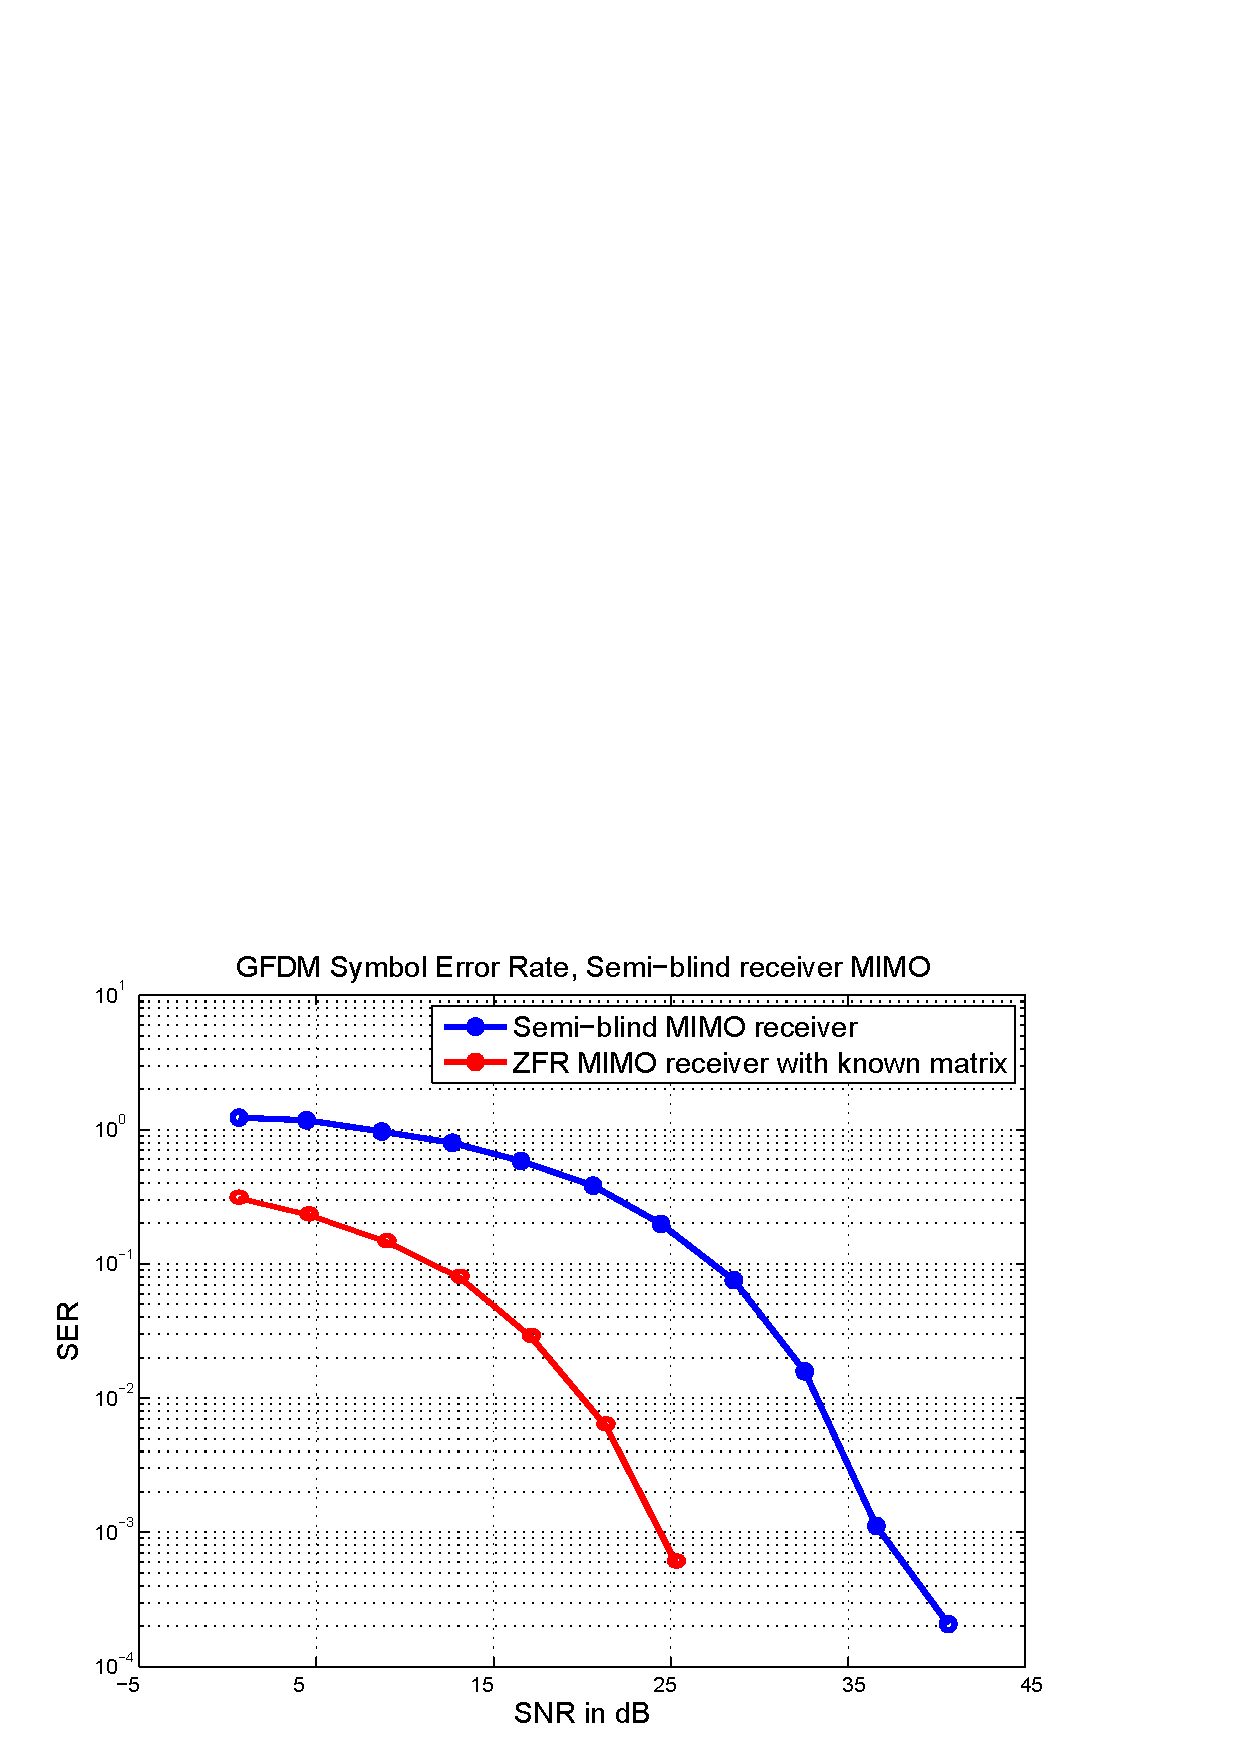
\includegraphics[width=0.9\columnwidth]{MIMO_SER_1.png}
\caption{\label{fig:fs_m_1}\textit{Производительность работы алгоритма поиска поднесущих для случая МВМВ}}
\end{figure}
\begin{figure}[H]
\centering
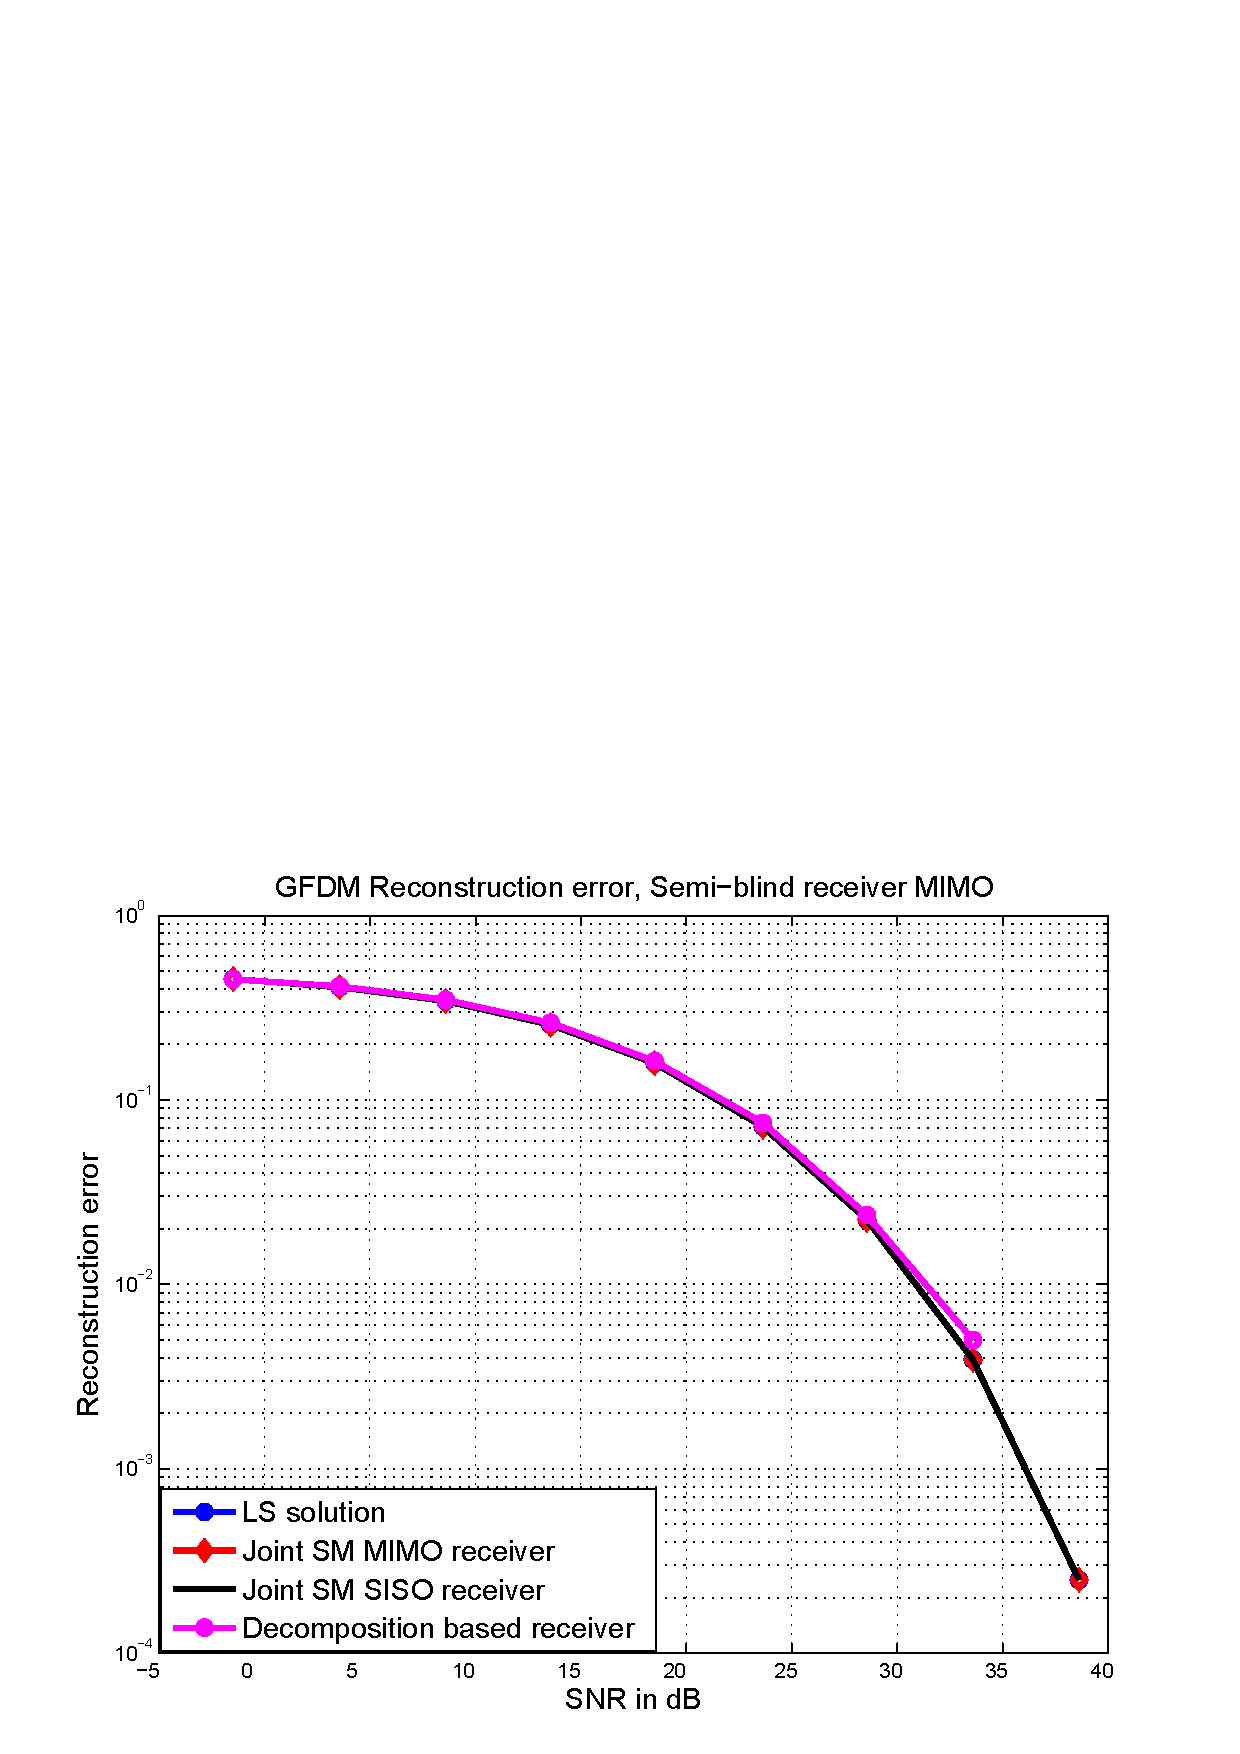
\includegraphics[width=0.9\columnwidth]{SM_RE_MIMO.png}
\caption{\label{fig:fs_m_2}\textit{Ошибка восстановления поднесущих для алгоритма поиска поднесущих для случая МВМВ}}
\end{figure}
Производительность системы ОбЧРК для работы алгоритма ортогонализации получены при помощи моделирования. В системе был положен аддитивный белый Гауссов шум без какого либо кодирования. В системе была использована квадратурная фазовая манипуляция. Количество поднесущих равно $F=16$. Количество временных отсчетов на каждый временной символ равно $T/T_s=F$. Количество временных символов равно $T_s=5$. В качестве фильтра был использован фильтр с характеристикой "Корень из приподнятого косинуса" с коэффициентом перекрытия $\alpha=0.5$. Коэффициенты канальной матрицы $\Amat$ были выбраны как случайные комплексные величины с нулевым моментом первого порядка и среднеквадратичным отклонением модуля числа равным $1$. В системе был использован приемник на основе псевдообратной матрицы. На первом  рисунке представлены результаты работы алгоритма по ортогонализации влияния канала. Мы сравнивали подход с МВМВ канальной ортогонализацией. Результаты показаны на  рис. для приемника на основе псевдообратной матрицы.
\begin{figure}[H]
\centering
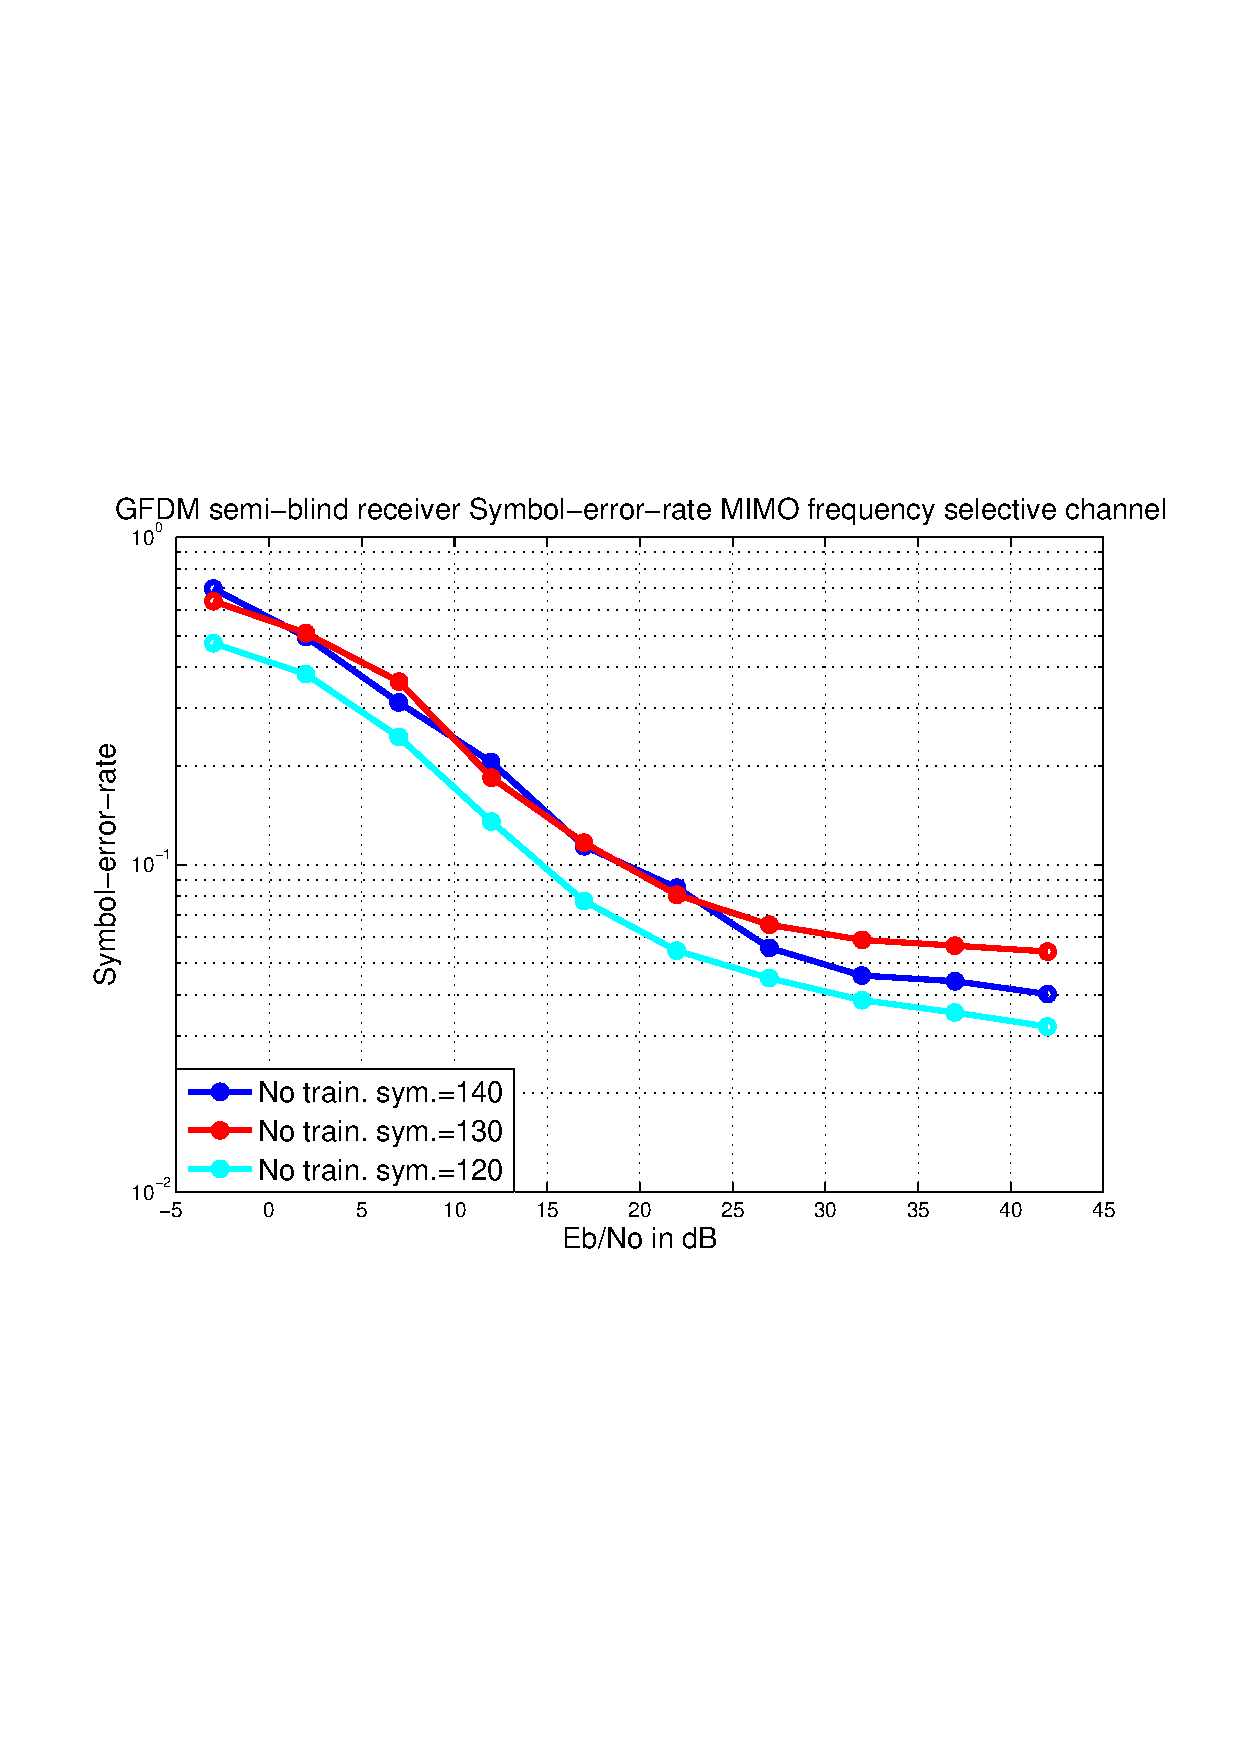
\includegraphics[width=0.9\columnwidth]{SM_MIMO_SER_ALS.png}
\caption{\textit{Производительность работы полу-слепого приемника для канала с памятью и системы МВМВ}}
\label{fig:fs_m_3}
\end{figure}
\begin{figure}[H]
\centering
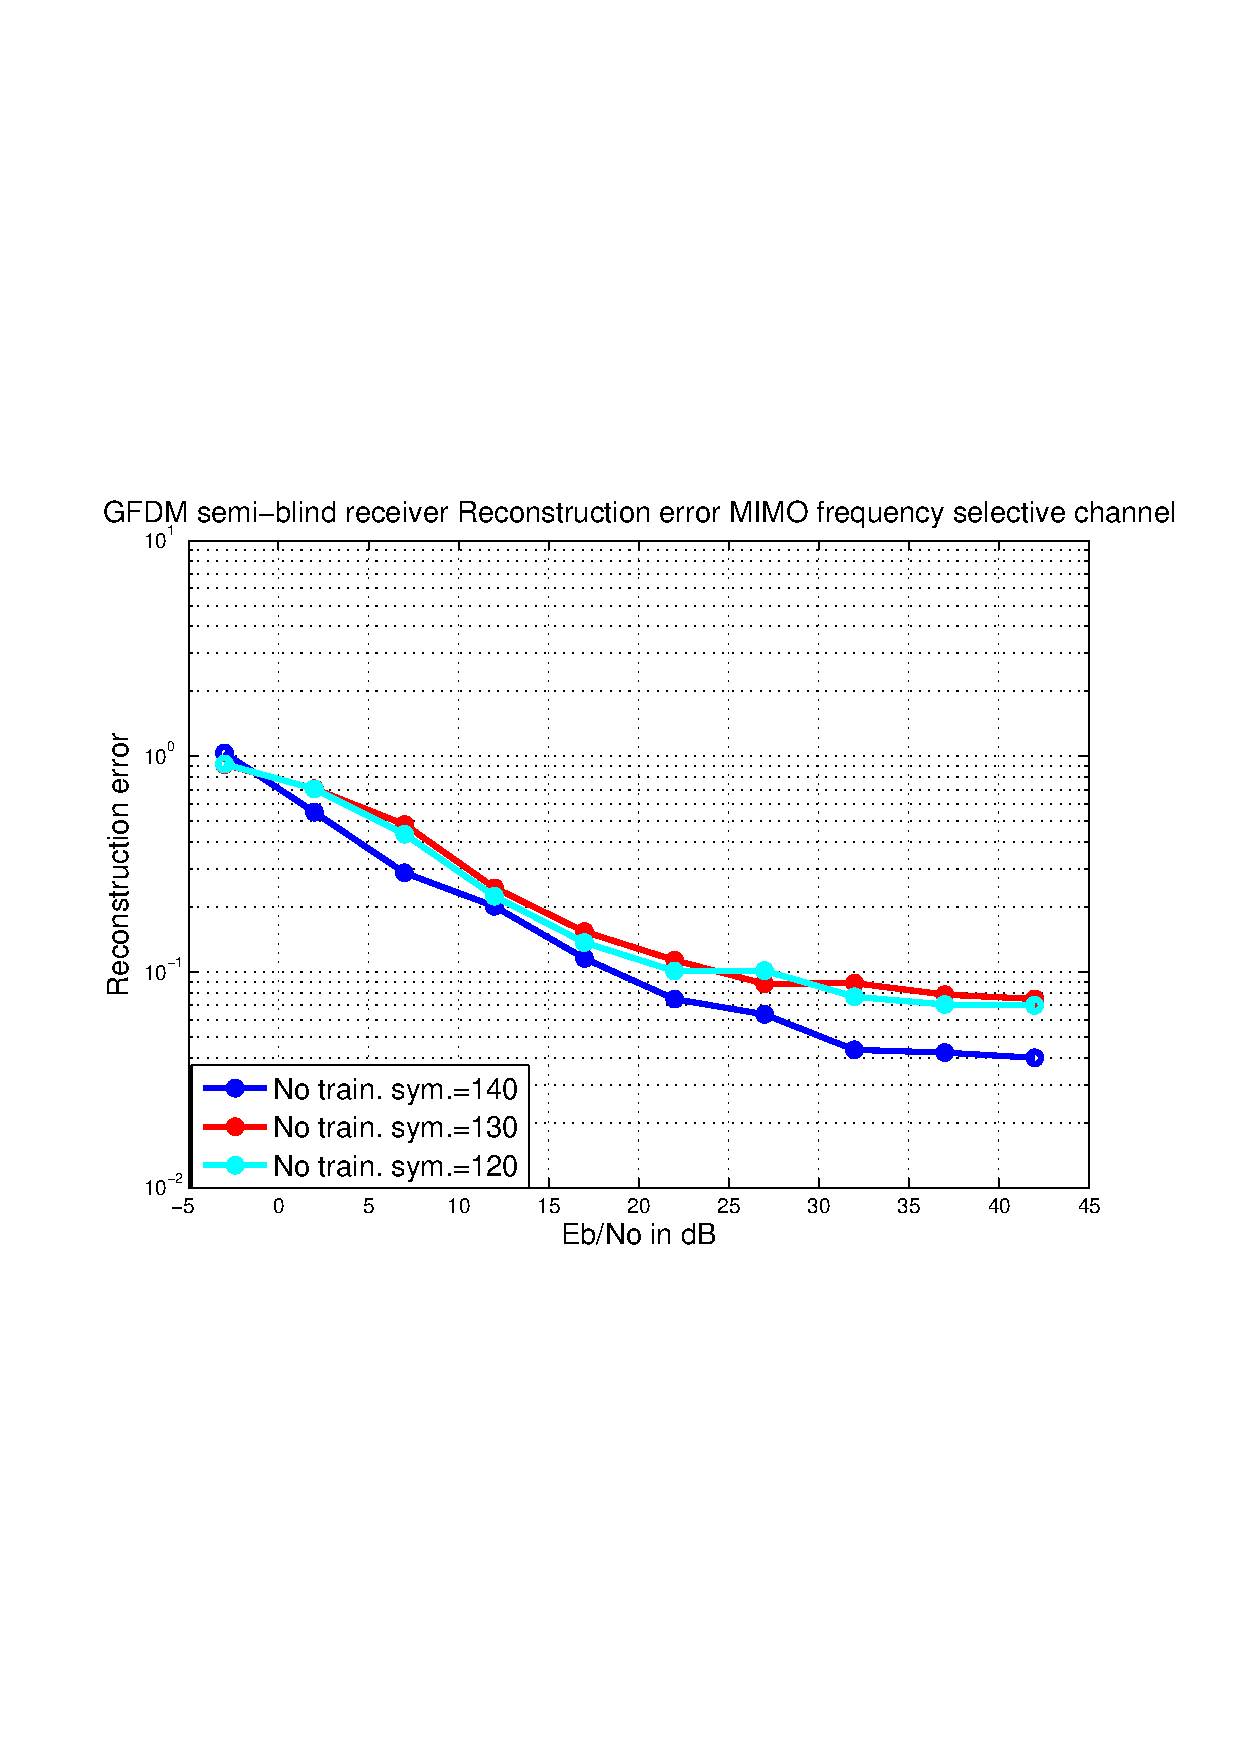
\includegraphics[width=0.9\columnwidth]{SM_MIMO_RE_ALS.png}
\caption{\textit{Ошибка восстановления канала полу-слепого приемника для канала с памятью и системы МВМВ}}
\label{fig:fs_m_4}
\end{figure}
Производительность системы ОбЧРК для сравнения поиска величин $\Amat$ коэффициентов получены при помощи моделирования. В системе был положен аддитивный белый Гауссов шум без какого либо кодирования. В системе была использована квадратурная фазовая манипуляция. Количество поднесущих равно $F=16$. Количество временных отсчетов на каждый временной символ равно $T/T_s=F$. Количество временных символов равно $T_s=5$. В качестве фильтра был использован фильтр с характеристикой "Корень из приподнятого косинуса" с коэффициентом перекрытия $\alpha=0.5$. Коэффициенты канальной матрицы $\Amat$ были выбраны как случайные целочисленные величины с возможными значениями равными 0 и 1. Результаты работы ОбЧРК представлены на двух рисунках, на первом показаны соотношения символов к количеству ошибок. Для сравнения так же показаны варианты когда система знает истинные коэффициенты матрицы $\mathbf{A}$ и находит решение на основе псевдообратной матрицы. На втором показана ошибка определения значения матрицы $\mathbf{A}$ нормализованное к истинной величине.
\begin{table}[H]
\caption{\label{tab:m_table3}ОбЧРК эксперимент 2.2}
\begin{center}
\begin{tabular}{|c|c|c|}
\hline
Параметр & Обозначение & Значение \\
\hline
\hline
Передающие антенны кол-во &$M_t$&2 \\
\hline
Приемные антенны кол-во  &$M_r$&2 \\
\hline
Схема модуляции & $\mu$ & 2(КФМ) \\
\hline
Отсчетов на символ & $T/T_s$ & 16 \\
\hline
Поднесущие &$F$&16 \\
\hline
Размер блока& $T_s$  &5 \\
\hline
Вид фильтра&  &КиПК \\
\hline
Коэффициент перекрытия&$\alpha$  &0.5 \\
\hline
Коэффициенты поднесущих & $\mathbf{a}_i$ & $randi([0 1])$ \\
\hline
Канал& $h$ &АБГШ \\
\hline
Префикс&  & Нет \\
\hline
Передача&  & Некодированная \\
\hline
Ранг разложения& $rank$ & 25\\
\hline
\end{tabular}
\end{center}
\end{table}
\begin{figure}[H]
\centering
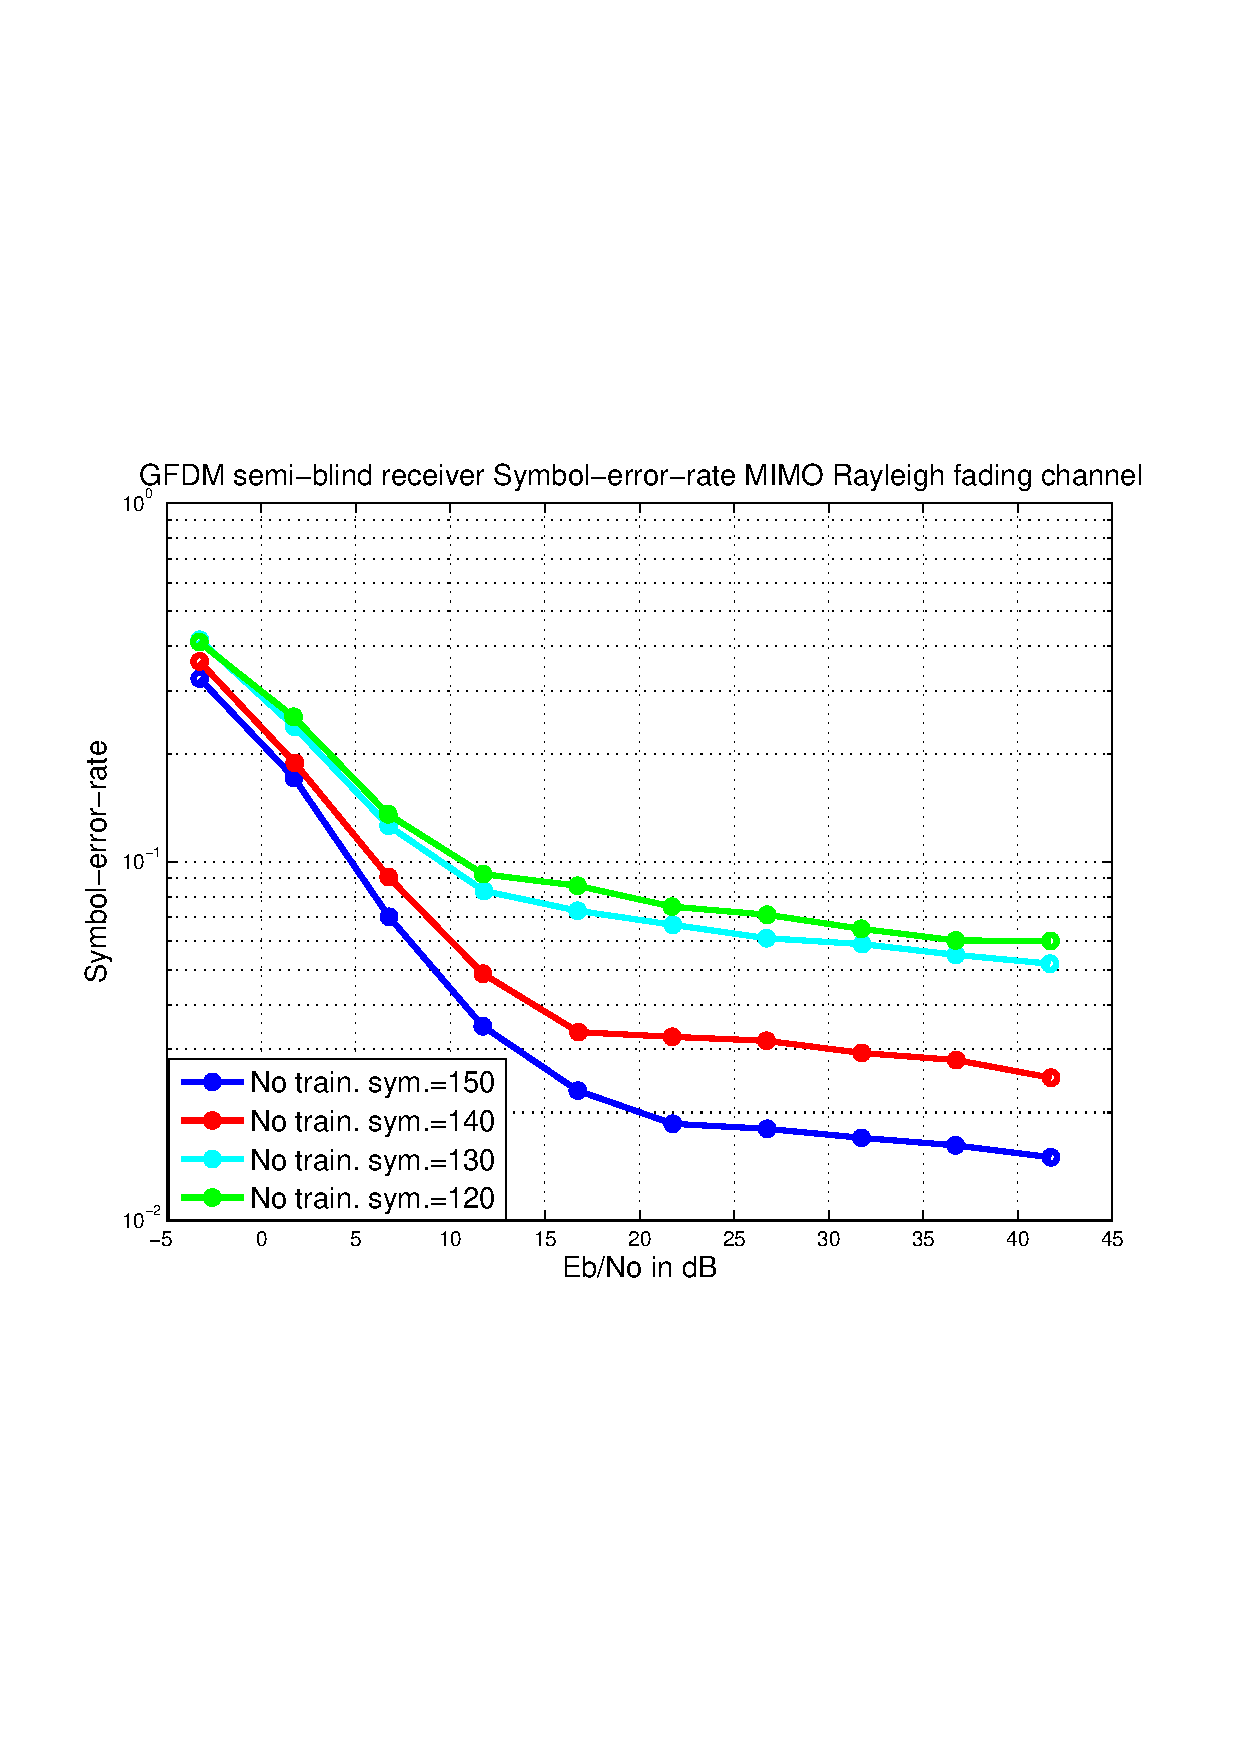
\includegraphics[width=0.9\columnwidth]{SM_MIMO_SER_N.png}
\caption{\textit{Производительность работы полу-слепого приемника для канала с памятью и системы МВМВ. Метод Ньютона}}
\label{fig:fs_m_5}
\end{figure}
\begin{figure}[H]
\centering
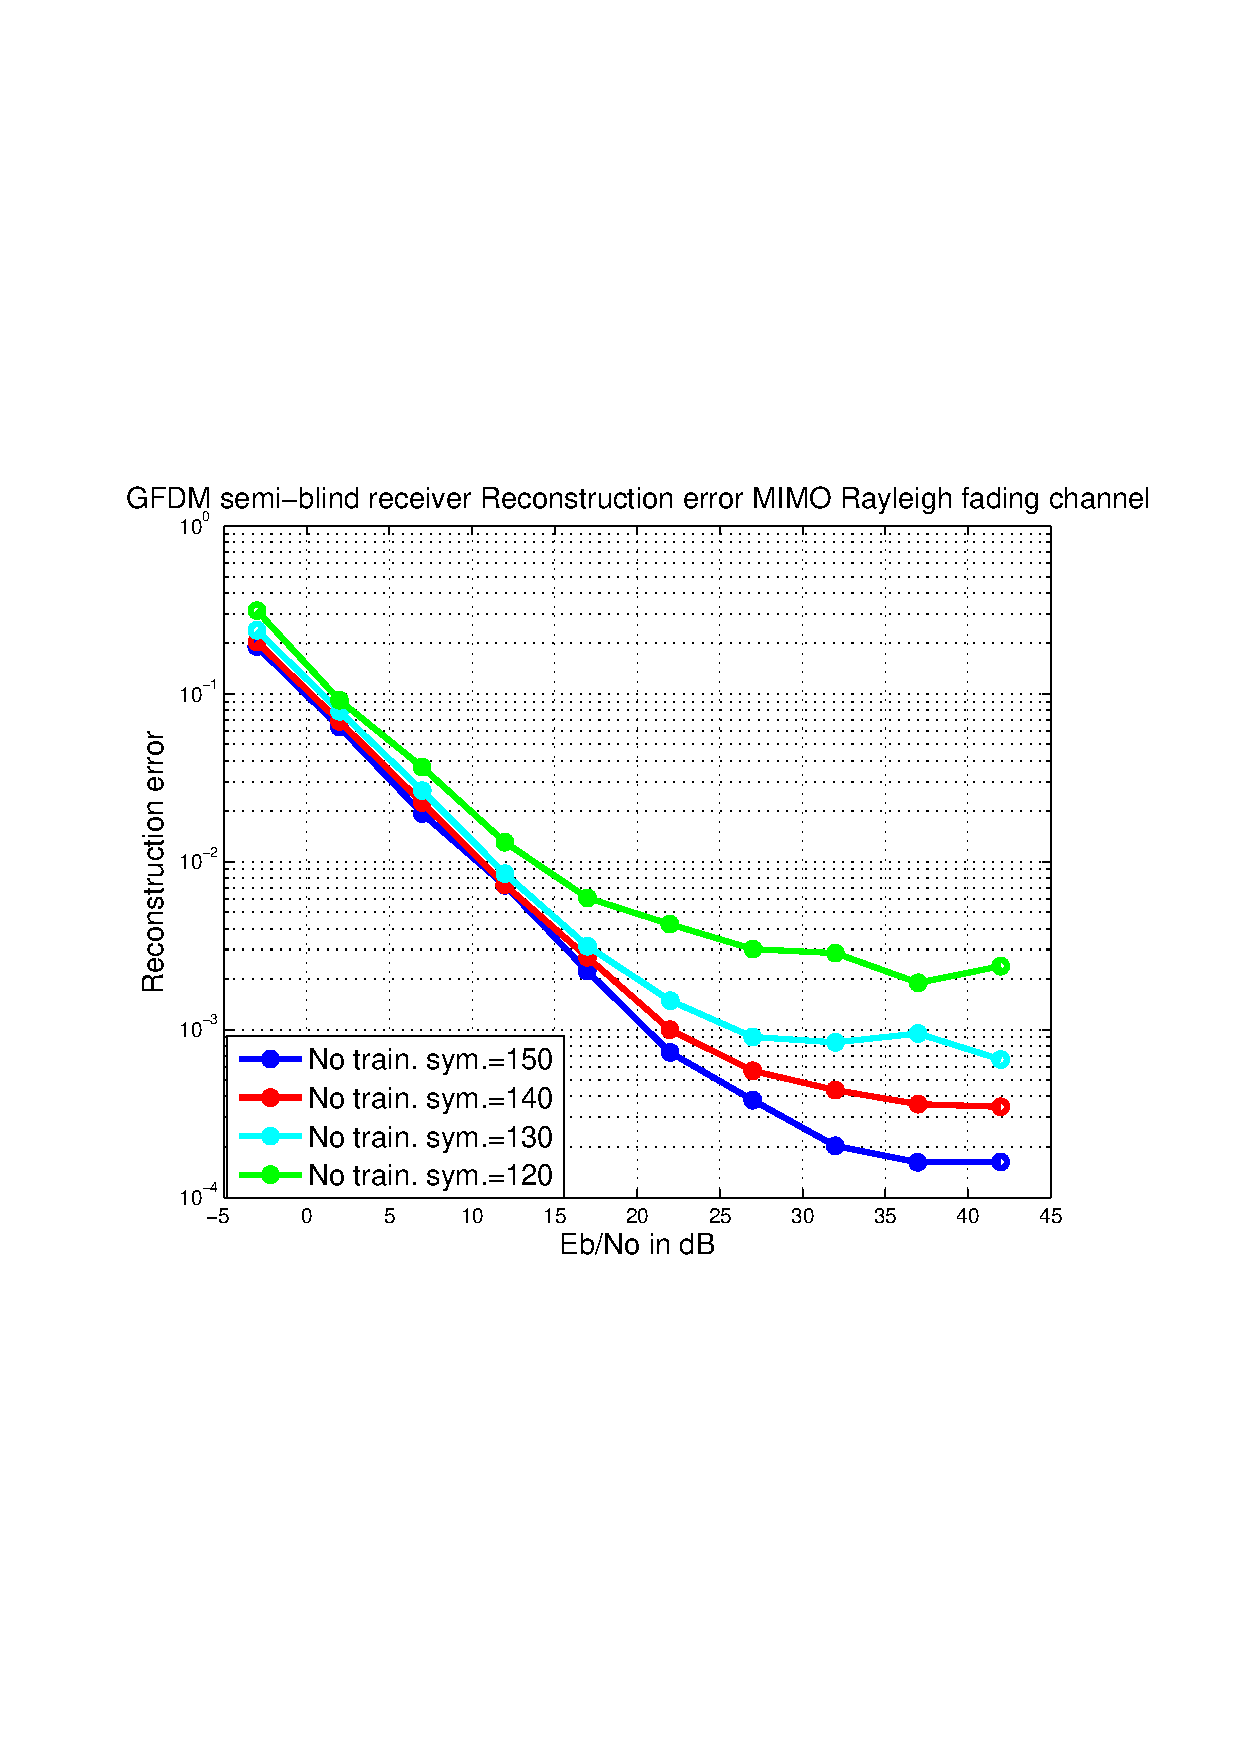
\includegraphics[width=0.9\columnwidth]{SM_MIMO_RE_N.png}
\caption{\textit{Ошибка восстановления канала полу-слепого приемника для канала с памятью и системы МВМВ. Метод Ньютона}}
\label{fig:fs_m_6}
\end{figure}
Полу-слепой приемник дял оценки канала и неизвестных символов основанный на методе Ньютона в системе МВМВ был оценен по производительности при помощи симуляции. Для симуляции была использована квадратурная фазовая модуляция. Канал был создан в два этапа: в качестве канала с памятью был использован канал $Ped-A$ из стандартов IEEE, в качестве модели различных антенн было использовано Рэлеевское замирание в канале. Для этого генерировалась матрица случайных комплексных величин $\mathcal{H}$ с дисперсией равной единице. После этого использовалось произведение по третьему пространству для получения канального тензора$\mathcal{H}$. Количество приемных и передающих антенн задано изначально $M_r=M_t=2$. Количество поднесущих было $F=16$, временных отсчетов на символ $T/T_s=F$. Размер блока был задан $T_s=5$. В качестве фильтра был использован корень из Приподнятого косинуса с коэффициентом перекрытия $\alpha=1$. Длина канала вычислялсь исходя из модели  и имела фиксированную длительность $L+1=4$. Параметры эксперимента так же представлены в табл.\ref{tab:m_table3}. Результаты производительности ОбЧРК показаны на двух графиках. На рис. \eqref{fig:fs_m_5} представлена производительность системы по распознаванию символов. Эксперимент показывает зависимость количества тренировочных символов в блоке и соотношения сигнал/шум. На рис.  \eqref{fig:fs_m_6} показана ошибка восстановления канала от аналогичных переменных.
Выражение для ошибка восстановления указано в \eqref{sim:eq_m_2}.
\begin{align}
R_e=\frac{\mid\mid\mathbf{h-\widehat{h}}\mid\mid^2}{\mid\mid\mathbf{h}\mid\mid^@}
\label{sim:eq_m_2}
\end{align}

\section{Заключение}
В первом эксперименте был исследован алгоритм поиска рабочих поднесущих в системе ОбЧРК с случае МВМВ. Как мы видим из результатов эксперимента, производительность по сравнению с эталоном для которого известны поднесущие упала на 5-6 дБ с точки зрения соотношения символы/ошибки. Данные результат виден из рис. \ref{fig:fs_m_2}. Падение в производительности связано с тем что в алгоритме был использован очень простой метод принятия решения по определению включенных поднесущих. Поскольку данная задача является задачей классификации, а мы используем регрессионный метод для поиска значений в алгоритме было использовано простейшее решающее устройство на основе порога. В случае если порог был меньше чем абсолютное значение оцениваемого коэффициента, поднесуащя считалась включенной. Таким образом используя более точные методы принятия решени можно добиться лучшего результата.

В качестве алгоритмов оценки поднесущих мы описали 3 различных алгоритма каждый из который действует различным методом, однако как показали результаты все они показывают одинаковую точность при принятии решений, что видно из рис.\ref{fig:fs_m_3} .Даже приближенный метод оценки позволяет оценить поднесущие с абсолютно той же точностью. Это может быть связано с тем, что решающее устройство на всех алгоритмах было одинаково, либо ошибка приближенного метода является несущественной. Однако следует отметить, что метод основанный на разложении чувствителен к выбору начальной точки, что делает сходимость алгоритма нестабильной. Из-за этого в результаты в графиках представлены в медианной оценке. Однако как можно видеть по медианной оценке, это не влияет на статистическую сходимость алгоритма.

Как видно из второго эксперимента полу-слепой приемник на основе алгоритмов ПМНК позволяет получать как символы так и оценивать состояние канала. Точность оценки к сожалению не высокая, что связано с достаточно сложными условиями приема, когда проявляется нестабильность соединения между антеннами, и проявления памяти канала для каждого из соединений. Как видно из рис.  \ref{fig:fs_m_3}, количество ошибок в системе ограничено снизу и производительность не оказывается лучше постоянного коэффициента. Более того аналогичный результат виден и в случае оценки состояния канала на рис. \ref{fig:fs_m_4}. Это связано с плохой обусловленностью системы. Кроме того состояние канала и коэффициенты связи между антеннами могут вместе получать эффект значительного ухудшения собственного числа матрицы канала. Таким образом как заключение к алгоритму можно сказать о необходимости использования регуляризующих коэффициентов. Поскольку задача является некорректно поставленной по Тихонову, можно использовать различные алгоритмы стабилизации решения у точки минимума. Однако можно сказать, что сама система имеет значительны потенциал и может показывать значительно лучшие результаты. Так же следует рассмотреть реальные модели канала МВМВ с памятью и типичные модели работы данного канала. Данные модели будут рассмотрены в дальнейшей работы.

Следующий эксперимент показывает производительность полу-слепого приемника на методе Ньютона. Канала вд данной модели полагается каналом с памятью модели $Ped-A$ взятый из стандарта IEEE умноженный по третьему пространству с матрицей случайных элементов с дисперсией равной единице. На рис. показана производительность алгоритма по распознаванию символов. Как видно из графика производительность алгоритма так же ограничена сверху и очень сильно зависит от количества тренировочных символов. Это связано с тем, что в относительном измерении количество канальных переменных велико. При этом от собственное число матрицы канала чрезвычайно велико и приводит к значительным погрешностям при работе алгоритма. Для устранения подобного влияния необходимо использование дополнительных методов как и было описано в предыдущем эксперимента. Однако в данном случае эти методы должны быть внедрены чрезвычайно аккуратно, так как метод второго порядка и очень чувствителен к возможным методам регуляризации.
Как видно из рис. точность определения канала значительно выше, чем символов и зависит в меньшей степени от количества символов. Количество тренировочных символов сказывается лишь на верхнем лимите. Данный эффект проявляется только при высоком соотношении сигнал/шум. В дальнейшей работе будут рассмотрены дополнительные алгоритмы по регуляризации и увеличению точности работы полу-слепого приемника а так же модели канала существующие в МВМВ системах. В качестве основных тезисов по работе полу-слепого приемника можно выделить следующее:
\begin{itemize}
\item Производительность приемника по распознаванию символов мала
\item Производительность приемника по оценке канала применима для работы в алгоритмах
\item Требуется использование регуляризирующих алгоритмов
\end{itemize}



%The last experiment show performance of the Newton based semi-blind receiver over the frequency selective Rayleigh fading channel. The fig.\eqref{fig:fs_m_5} show the performance of the algorithm in the symbol estimation. As we can see here the algorithm has the upper bound in the performance and doesn't allow to decrease the SER lower than $10^{-2}$. This behavior doesn't connected with error in the channel estimation, because the error in the channel estimation is upper bounded with much higher SNR and have precision near to the $10^{-3}$/ The main reason for this behavior is the high condition number of the Jacobian matrix. To implement the more precise and regularized solution the BFGS of Levenberg-Marquardt algorithm must be applied. We can see from the results, that there is significant dependency between the  number of the training symbols and performance of the system. The number of the training symbols is high due to the high number of estimated channel variables.The fig.\eqref{fig:fs_m_6} show the performance of the algorithm in the channel estimation. We can see that precision of the algorithm is high and algorithm estimates the channel with precision up to $10^{-3}$ reconstruction error. There are disadvantages of the algorithm which connected with bad conditioning and the computational complexity. The additional approaches must be investigated to overcome them. As conclusion for this algorithm we can propose two statements:
%\begin{itemize}
%\item Performance of the algorithm weak for the symbols estimation
%\item Performance of the algorithm applicable for the channel estimation
%\item The algorithm must use the regularizing approach.
%\end{itemize}
%There are many frequency coefficients estimation approaches and we compares the separately, but all of them has the same result as we can see from the fig. \ref{fig:fs_m_3}. Even the solution based on the approximated SISO model show the same result. This behaviour come from the additional channel estimation with limit which decrease influence of the noise but also decrease the performance of the more powerful algorithms. Also it should be noted that the joint MIMO algorithm allow to also the symbol estimation, and other algorithms can't estimate the symbols in the received data. The difference between explained algorithms is significant due to the assumptions which was in each of the approaches to estimate $\mathbf{A}$.
% 
%The main assumption of the SISO semi-blind based approach is error spread between transmit antennas. We ignored unknown values because unknown symbols at the receiver doesn't used. Repetition of the algorithm for the each transmit antenna allow to estimate coefficients for the sub-carrier selection matrix. Assumption is not applied for the time slots due to the overlapping and the receiver estimates the coefficient approximately. The error depends from the difference between sub-carrier selection coefficients in the each transmit antenna due to the time slot mixing in the GFDM systems. The SISO semi-blind based approach is the most expensive algorithm in comparison with others. The receiver can estimate parallel solution for the each sub-carrier selection coefficient corresponding to the each transmit antenna. The parallel solution decreases iteration time of the approach.
%
%The algorithm based on the least squares solution achieve the better results. The approach doesn't have assumptions in the mathematical model  for the GFDM system. But the least squares solution is very sensitive to the condition number of the matrix. The least squares solution is expensive too.
%
%The decomposition based approach of the unfolding multiplication with the matrix decrease size of the problem.  There is trade of between complexity of the task and calculation of the optimization process. Each iteration contain the matrix inversion inside. The matrix to invert change every iteration change from iteration to iteration.
%We can see that result of the all three algorithms is the same. There is significant difference for the decomposition based approach if we use the mean value metric. because we can choose bas initial point. Therefore we used the median value metric.
%
%Next experiment is the semi-blind receiver channel and the symbol estimation over frequency selective Rayleigh fading channel. The experiment was done for the all possible number of known symbols which have solution for the problem statement. The result for the SER if shown in the fig. \ref{fig:fs_m_3}. As we can see here, there is one optimal point in symbol estimation. The less unknown symbols in the block increase the SNR, whether the higher number of unknown symbols decrease performance of the approach. The solution where number of unknown symbols equal to $8$ show the closest result to the original GFDM system with the same block size, known channel and zero forced receiver. The channel reconstruction error has the similar behaviour and show the optimal point in the same number of unknown symbols. Important fact is that reconstruction error for the maximal and minimal number of unknown have different behaviour in comparison with the SISO model. But this behaviour also show the convexity of the performance function for the number of unknown symbols as variable. The different block size should have different optimal value of the unknown symbols, but the average performance must be the worse from the known channel system due to the higher energy per bit with same performance. 
%The last experiment is the semi-blind receiver channel and the symbol estimation over frequency selective Rayleigh fading channel  with the Newton based approach. The experiment was done for the all possible number of known symbols which have solution for the problem statement. The result for the SER if shown in the fig. \ref{fig:fs_m_5}. 
%
%
\input{conc_new.tex}
%\input{Intro.tex}
%\chapter{Generalized frequency division multiplexing multiple input multiple output}\label{sec:GFDMMIMO}
\section{System model}\label{part:SM1}
In this chapter we assume the GFDM MIMO system  the flat-frequency channel\cite{Book25}\cite{Book29} in that case the system is explained in the 
\eqref{mim_1} equation with channel model a identity matrix without multipath propagation.
\begin{align}
\mathbf{Y}=\mathbf{HZ}+\mathbf{N}
\label{mim_1}
\end{align}
\begin{align*}
\mathbf{H}\in\compl^{M_r\times M_t}
\mathbf{Z}\in\compl^{M_t\times T}
\mathbf{N,Y}\in\compl^{M_r\times T}
\end{align*}
%\subsection{MIMO model}
The GFDM system in MIMO AWGN case can be explained with the PARATUCK2 third order model. The difference between the SISO and MIMO case is significant\cite{Book29}, but PARATUCK2 model allow to extend  matrices to define the MIMO case inside of the same mathematical structure. The received data should have certain dimensionality $\mathbf{Y}\in\compl^{M_r\times T}$
The symbol matrix $\mathbf{S}$ from the SISO system become three dimensional tensor $\mathcal{S}\in\compl^{F\times T_s\times M_t}$ in the MIMO case. Additional dimension corresponds to the symbols which is transmitted from the different transmit antennas. The PARATUCK2 does not allow using tensors in the model. To overcome this constraint we transform the $\mathcal{X}$ into the stacked slices for each $m_t$ \eqref{mimo_1}.
\begin{align}
\mathbf{S}=\begin{bmatrix}
\mathcal{S}_{:,:,1}\\
\mathcal{S}_{:,:,2}\\
\vdots \\
\mathcal{S}_{:,:,M_t}\\
\end{bmatrix} \label{mimo_1}
\end{align}
\begin{align*}
\mathcal{S}\in\compl^{F\times T_s\times M_t}
\mathbf{S}\in\compl^{F\cdot M_t\times T_s}
\end{align*}
The $C^{[b]}$ matrix stay the same as in the SISO model and does not change with increasing of the transmit antennas \eqref{mim_2}. In the columns of the matrix stays the same time mixing filter which doesn't change from the number of the transmit and receive antennas. From the right hand side the $\mathbf{S}$ does not change and have number of the columns $T_s$ which also satisfy the model.
\begin{align}
\mathbf{C}^{[b]}\in\compl^{T\times T_s}
\label{mim_2}
\end{align}
The connection array $\mathbf{b}$ stay the same as in the SISO case \eqref{mimo_3}. The necessary assumption for this is linear time invariant transmission channel in terms of the one transmission block. We fill the $\mathbf{b}$ array with all-ones as in the SISO case.
\begin{align}
\mathbf{b}=\mathbf{1}_{T_s\times 1} \label{mimo_3}
\end{align}
\begin{align*}
\mathbf{b} \in\compl^{T_s\times 1} 
\end{align*}
The $\mathbf{C}^{[a]}$ matrix in the MIMO case is changed \eqref{mimo_4}. Define this matrix in the MIMO case as $\mathbf{C}^{[a]'}$. Regarding to the $\mathbf{S}$ matrix, dimensions of the $\mathbf{C}^{[a]'}$ should be $T \times F\cdot M_t$. In comparison with the SISO model, in the MIMO case $\mathbf{S}$ should be multiplied with the $\mathbf{C}^{[a]}$ matrices. The new $\mathbf{C}^{[a]'}$ become stacked repeated version of the $\mathbf{C}^{[a]}$ matrix \eqref{mimo_5}. Hadamard product between $\mathbf{S}$ and the $\mathbf{C}^{[a]'}$ become simple explanation of the sub-carrier modulation of the each sub-frequency at the each transmitter antenna. Sub-carriers in the each transmit antennas is equal, so $\mathbf{C}^{[a]}$ matrices for each $m_t$ is also equal.
\begin{align}
\mathbf{C}^{[a]'}=
\begin{bmatrix}
\mathbf{C}^{[a]}& \mathbf{C}^{[a]}& \cdots &\mathbf{C}^{[a]}\\
\end{bmatrix} \in\compl^{T\times M_t\cdot F} \label{mimo_4}
\end{align}
\begin{align}
\mathbf{C}^{[a]'}=(\mathbf{1}_{1\times M_t} \otimes \mathbf{C}^{[a]}) \in \compl^{  T\times M_t\cdot F} \label{mimo_5}
\end{align}
The $\mathbf{a}$ array become the matrix and connect each $m_r$ antenna with the each $m_t$ transmit antenna and include every sub-carrier coefficient\eqref{mimo_6}. Define sub-carrier coefficients as the $\mathcal{A}$ tensor with coefficients for each $m_r,m_t,f$. In the PARATUCK2 model $\mathbf{A}$ is the matrix, we must define the $\mathcal{A}$ as the matrix which will sum for every transmit antenna sub-carrier frequency with corresponding sub-carrier coefficient\eqref{mimo_7}. Regarding to the $\mathbf{S}$ matrix, symbols is located sequentially for each sub-carrier at each transmit antenna. The $\mathbf{A}$ dimension is $M_r \times F\cdot M_t$. The first unfolding of the $\mathcal{A}$ have corresponding sub-carrier coefficients following the $\mathbf{S}$ symbols\eqref{mimo_8}. This notation multiplies each sub-carrier coefficient $\mathbf{A}$ to each symbol from the $\mathbf{S}$.
\begin{align}
\mathcal{A} \in \compl^{M_r\times F\times M_t} \label{mimo_6}
\end{align}
\begin{align}
\mathbf{A}=\mathcal{A}_{[1]} \label{mimo_7}
\end{align}
\begin{align}
\mathbf{A}\in\compl^{M_r \times F\cdot M_t} \label{mimo_8}
\end{align}
The overall model with explained matrices will be defined in the \eqref{mimo_9}. This model define the received data. All operation, which was explained in the GFDM SISO part is also applicable in the GFDM MIMO case. It should be noted that the rank of the $\mathbf{A}$ is $min(M_r,F\cdot M_t)$ in the real case number of the receive antennas is much less than sub-carriers multiplied with transmit antennas. The rank of the matrix $\mathbf{A}$ show how many transmit coefficient possible to know in the system with known transmitted symbols.
\begin{align}
\mathbf{HZ}=\mathbf{X}=\mathbf{A}\cdot (\mathbf{C}^{[a]'T} \odot (\mathbf{S}\cdot (\mathbf{C}^{[b]}\diamond \mathbf{B})^T)) \label{mimo_9}
\end{align}
\begin{align*}
\mathbf{X}\in\compl^{M_r \times T}
\mathbf{A}\in\compl^{M_r \times F\cdot M_t}
\mathbf{C}^{[a]'}\in\compl^{T \times F\cdot M_t}
\end{align*}
\begin{align*}
\mathbf{S}\in\compl^{F\cdot M_t \times T_s}
\mathbf{C}^{[b]}\in\compl^{T \times T_s}
\mathbf{B}\in\compl^{1 \times T_s}
\end{align*}

\section{Sub-carrier coefficient update approach}\label{part:SCUA}
The spectrum sensing approach is applicable in the MIMO system too. One of the important properties in the MIMO system is diversity, which frequently achieved via spatial location of the transmitter and receiver antennas\cite{Book29}. It should be noted that for different transmitter-receiver antenna pair one sub-carrier may be occupied with another system, and not. Receiver must know the $\mathbf{A}$ to know how data is transmitted. Sub-carrier coefficients update is complex task due to the time mix and multi-frequency system. The number of the unknown variables in the system for MIMO case equal to the $M_r\cdot M_t\cdot F$. Number of the equations to solve equal to the $T\cdot M_r$ for each transmission block. The transmission coefficients can be found with specially structured known symbol matrix. 
\subsection{Approximated approach}
The one way to find the matrix $\mathbf{A}$ with sub-carrier coefficients is semi-blind receiver. The number of time slots must equal to the number of the transmit antennas. The receiver may use approach from the previous chapter \ref{part:SCSSISO}. Transmitter should construct special structure of the matrix $\mathbf{S}$. For each time slot the receiver can find the $M_r\cdot F$ transmission coefficients. The transmitter must fill at least $M_t$ time slots with known symbols to find the all $\mathbf{A}$ matrix. The search algorithm for the  matrix $\mathbf{A}$ is next:
\begin{itemize}
\item Transmitter put inside the transmission block specially structured symbols. Transmitter put known to the receiver symbol row to the one transmit antenna at the each time slot. In other words the symbols are sent from each sub-carrier frequency in the certain antenna.  Transmitter repeats the same row, but from another transmit antenna at the next time slot. The transmitter repeat process $M_t$ times for each antenna. The receiver must know the   transmission order. 
\item  The receiver has transmission block with $M_t$ time slots length. The receiver uses semi-blind approach from the SISO case and assume received signal is sent from the SISO system. Semi-blind receiver approach estimates the sub-carrier coefficients for $m_t$-th transmit antenna.
\item The receiver repeats process for another time slot, and estimates the sub-carrier coefficients for another transmit antenna. The receiver repeats process $M_t$ times until estimates the all $\mathbf{A}$ matrix elements.
\end{itemize}
\subsection{MIMO model based approach}
The matrix $\mathbf{A}$ will be found with the equation \eqref{mimo_msm_4} separation  in the PARATUCK2 model. The model is written as the vectorized matrix $\mathbf{A}$ multiplication with the intermediate matrix $\mathbf{\Delta}$, as given in \eqref{mimo_msm_5}. 
\begin{align}
\mathbf{Y}=\mathbf{HZ}+\mathbf{N} \label{mimo_msm_1}
\end{align}
\begin{align}
\mathbf{HZ}=\mathbf{X}=\mathbf{A}\cdot (\mathbf{C}^{[a]'T} \odot (\mathbf{S}\cdot (\mathbf{C}^{[b]}\diamond \mathbf{b}^T)^T)) \label{mimo_msm_2}
\end{align}
\begin{align*}
\mathbf{Y,X,N}\in\compl^{M_r\times T}
\mathbf{H}\in\compl^{M_r\times M_t}
\mathbf{Z}\in\compl^{M_t\times T}
\end{align*}
\begin{align}
vec(\mathbf{\widehat{X}})=vec(\mathbf{\widehat{A}}\cdot (\mathbf{C}^{[a]'T} \odot (\mathbf{S}\cdot (\mathbf{C}^{[b]}\diamond \mathbf{B})^T))) \label{mimo_msm_3}
\end{align}
 The product of this two matrices explained in the vectorized form for both of the second matrices \eqref{mimo_msm_4}.The matrix $\mathbf{\Delta}$ constructed with property \eqref{mimo_msm_4} and defined in \eqref{mimo_msm_5}.  We used property \eqref{mimo_msm_4} to find the sub-carrier coefficient matrix $\mathbf{A}$ from the received data. The overall equation is defined as \eqref{mimo_msm_6}.
\begin{align}
vec(\mathbf{OP})=(\mathbf{P}^T \otimes \mathbf{I})\cdot vec(\mathbf{O}) \label{mimo_msm_4}
\end{align}
\begin{align}
\mathbf{\Delta}=(\mathbf{C}^{[a]'T} \odot (\mathbf{S}\cdot (\mathbf{C}^{[b]}\diamond \mathbf{B})^T)) \label{mimo_msm_5}
\end{align}
\begin{align}
vec(\mathbf{\widehat{X}})=(\mathbf{\Delta}^T\otimes \mathbf{I})\cdot vec(\mathbf{\widehat{A}}) \label{mimo_msm_6}
\end{align}
 We constructed the objective function to minimize the second norm of the vectorized residual explained via $vec(\mathbf{A})$ array \eqref{mimo_msm_6}. The function is non-holomorphic\cite{Book58} due to the complex values in the  $vec(\mathbf{A})$. We have used Wirtinger calculus and have found the first partial derivative. We have equated first partial derivative to the zero\cite{Book47}. The first partial derivative has global minimum point, because the second norm  function is convex. 

\begin{align}
\mathbf{r}_5=vec(\mathbf{Y})-vec(\mathbf{\widehat{X}}) \label{mimo_msm_7}
\end{align}
\begin{align*}
\mathbf{\Delta}\in\compl^{M_t\cdot F\times T}
\mathbf{r}_5\in\compl^{M_r\cdot T\times 1}
\end{align*}
\begin{align}
\min_{vec(\mathbf{A})}\mathbf{r}_5^H\mathbf{r}_5 \label{mimo_msm_8}
\end{align}
\begin{align}
\frac{\delta \mathbf{r}_5^H\mathbf{r}_5}{ \delta vec(\mathbf{\widehat{A}}^*)}=0 \label{mimo_msm_9}
\end{align}
\begin{align}
\frac{\delta \mathbf{r}_5^H\mathbf{r}_5}{ \delta vec(\mathbf{\widehat{A}}^*)}=\frac{\delta (vec(\mathbf{Y})-vec(\mathbf{\widehat{X}}))^H(vec(\mathbf{Y})-vec(\mathbf{\widehat{X}}))}{\delta vec(\mathbf{\widehat{A}}^*)}\label{mimo_msm_10}
\end{align}
\begin{align}
\frac{\delta \mathbf{r}_5^H\mathbf{r}_5}{ \delta vec(\mathbf{\widehat{A}}^*)} =(\mathbf{\Delta}^T\otimes \mathbf{I})^H(\mathbf{\Delta}^T\otimes \mathbf{I})vec(\mathbf{\widehat{A}})-(\mathbf{I}\otimes \mathbf{\Delta})^H vec(\mathbf{Y})=0 \label{mimo_msm_11}
\end{align}
\begin{align}
(\mathbf{\Delta}^T\otimes \mathbf{I})^H(\mathbf{\Delta}^T\otimes \mathbf{I})vec(\mathbf{\widehat{A}})=(\mathbf{\Delta}^T\otimes \mathbf{I})^H vec(\mathbf{Y}) \label{mimo_msm_12}
\end{align}
\begin{align}
vec(\mathbf{\widehat{A}})_{opt}=((\mathbf{\Delta}^T\otimes \mathbf{I})^H (\mathbf{\Delta}^T\otimes \mathbf{I}))^{-1}
(\mathbf{\Delta}^T\otimes \mathbf{I})^H vec(\mathbf{Y}) \label{mimo_msm_13}
\end{align}
\begin{align}
vec(\mathbf{\widehat{A}})_{opt}=((\mathbf{\Delta}^*\otimes \mathbf{I}) (\mathbf{\Delta}^T\otimes \mathbf{I}))^{-1}
(\mathbf{\Delta}^*\otimes \mathbf{I}) vec(\mathbf{Y}) \label{mimo_msm_14}
\end{align}
 The optimal solution in the second norm sense is written as here \eqref{mimo_msm_15}. We can simplify defined equation \eqref{mimo_msm_15} with  linear algebra properties. The simplified equation is defined as \eqref{mimo_msm_17}
\begin{align}
vec(\mathbf{\widehat{A}})_{opt}=((\mathbf{\Delta}^*\mathbf{\Delta}^T) \otimes \mathbf{I})^{-1}(\mathbf{\Delta}^*\otimes \mathbf{I}) vec(\mathbf{Y}) \label{mimo_msm_15}
\end{align}
\begin{align}
vec(\mathbf{\widehat{A}})_{opt}=((\mathbf{\Delta}^*\mathbf{\Delta}^T)^{-1} \otimes \mathbf{I}^{-1})(\mathbf{\Delta}^*\otimes \mathbf{I}) vec(\mathbf{Y}) \label{mimo_msm_16}
\end{align}
\begin{align}
vec(\mathbf{\widehat{A}})_{opt}=((\mathbf{\Delta}^*\mathbf{\Delta}^T)^{-1}\mathbf{\Delta}^* \otimes \mathbf{I}) vec(\mathbf{Y}) \label{mimo_msm_17}
\end{align}
We applied the Kronecker product properties and have analysed the rank of the inverse matrix $((\mathbf{\Delta}^*\mathbf{\Delta}^T)^{-1} \otimes \mathbf{I}^{-1})(\mathbf{\Delta}^*\otimes \mathbf{I})$ to find number of the coefficients which is possible to estimate in the one transmission block \eqref{mimo_msm_17}. The rank of the Kronecker product equals to the product between the multiplied matrix ranks \eqref{mimo_msm_rank_1}. The identity matrix has the maximal rank, so the rank of the matrix is defined by the second part of the equation \eqref{mimo_msm_rank_3}. Consider the matrix \eqref{mimo_msm_5}, The size of the core matrix $\mathbf{S}$ is equal to the $M_t\cdot F\times T_s$ , rank of the matrix $(\mathbf{S}\cdot (\mathbf{C}^{[b]}\diamond \mathbf{B})^T)$ is less of equal to the $T_s$. There is inequality which define the rank of the Hadamard product \eqref{mimo_msm_rank_5} as written in the \cite{Book48}\cite{Book56}\cite{Book57}. The matrix $\mathbf{C}^{[a]'T}$ has the rank equal to the $min(F,T)$ because it based on the stacked repetition of the $\mathbf{C}^{[a]T}$ matrix. The $\mathbf{C}^{[a]T}$ matrix has the full rank $min(F,T)$. The matrix \eqref{mimo_msm_rank_6} has the rank equal to the matrix $\mathbf{\Delta}$ rank. We have defined the system of the linear equations rank with equation \eqref{mimo_msm_rank_7}.
\begin{align}
rank(\mathbf{\Delta}^*\mathbf{\Delta}^T)^{-1}\mathbf{\Delta}^*\otimes \mathbf{I}) =(rank(\mathbf{I}))rank((\mathbf{\Delta}^*\mathbf{\Delta}^T)^{-1}\mathbf{\Delta}^*) \label{mimo_msm_rank_1}
\end{align}
\begin{align}
rank(\mathbf{I})=M_r \label{mimo_msm_rank_2}
\end{align}
\begin{align}
rank((\mathbf{\Delta}^*\mathbf{\Delta}^T)^{-1}\mathbf{\Delta}^*)) = rank(\mathbf{\Delta})\label{mimo_msm_rank_3}
\end{align}
\begin{align}
rank(\mathbf{\Delta})\leq rank(\mathbf{C}^{[a]'T})rank((\mathbf{S}\cdot (\mathbf{C}^{[b]}\diamond \mathbf{B})^T)))\label{mimo_msm_rank_4}
\end{align}
\begin{align}
rank(\mathbf{C}^{[a]'T}) =min(T_s,F) \label{mimo_msm_rank_5}
\end{align}
\begin{align}
rank((\mathbf{S}\cdot (\mathbf{C}^{[b]}\diamond \mathbf{B})^T))) = rank(\mathbf{S}) \leq T_s\label{mimo_msm_rank_6}
\end{align}
\begin{align}
rank((\mathbf{\Delta}^H\mathbf{\Delta})^{-1}\mathbf{\Delta}^H)) \leq T_s \cdot min(T_s,F) \label{mimo_msm_rank_7}
\end{align}
\begin{align}
rank(((\mathbf{\Delta}^*\mathbf{\Delta}^T)^{-1}\mathbf{\Delta}^* \otimes \mathbf{I}) ) \leq  T_s\cdot M_t \cdot min(T_s,F)\label{mimo_msm_rank_8}
\end{align}
The transmitter can use the specially structured symbol matrix as explained in the semi-blind receiver for SISO case part. We will find the all matrix $\mathbf{A}$ via least squares solution.We consider all dependencies with the MIMO based approach. We don't make assumption about SISO case and hold precision of the estimation.
\subsection{Decomposition based approach}
The receiver can estimate sub-carrier selection coefficients with less number of unknowns. The tensor $\mathcal{A}$ from the PARATUCK2 model is explained as unfolding of tensor decomposition and decrease number of estimated variables.
\begin{align}
\mathbf{Y}=\mathbf{HZ}+\mathbf{N}=\mathbf{X}+\mathbf{N}\label{mimo_dsm_1}
\end{align}
\begin{align}
\mathbf{HZ}=\mathbf{X}=\mathbf{A}\cdot (\mathbf{C}^{[a]'T} \odot (\mathbf{S}\cdot (\mathbf{C}^{[b]}\diamond \mathbf{b}^T)^T))\label{mimo_dsm_2}
\end{align}
\begin{align}
\mathbf{A}=\mathcal{A}_{[1]}=\mathbf{A_A}\cdot(\mathbf{A_C}\diamond \mathbf{A_B})^T\label{mimo_dsm_3}
\end{align}
\begin{align}
\mathbf{X}=\mathbf{A}_A\cdot(\mathbf{A}_C \diamond \mathbf{A}_B)^T \cdot \mathbf{C}^{[a]'T} \odot (\mathbf{S}\cdot (\mathbf{C}^{[b]}\diamond \mathbf{b}^T)^T)) \label{mimo_dsm_4}
\end{align}
\begin{align*}
\mathcal{A} \in \compl^{M_r\times F\times M_t}
\end{align*}
where $\mathbf{A}_A \in\compl^{M_r\times r} \mathbf{A}_B \in\compl^{F\times r} \mathbf{A}_C \in\compl^{M_t\times r}$ and therefore receiver decrease number of variables to solve the task\eqref{mimo_dsm_5} where we must find the $N_1$ variables. In case of the decomposition approach the number of the estimated values is expressed with another equation \eqref{mimo_dsm_6}, where previous variables come in the sum, but we add new variable which we can adjust. Relation from $r$ to possible decrease of necessary equations grows polynomially. Rank of the decomposition decrease number of the variables in case if $r$ from the \eqref{mimo_dsm_7} will be higher than rank of the tensor decomposition.

\begin{align}
N_1=M_r\cdot M_t\cdot F \label{mimo_dsm_5}
\end{align}
\begin{align}
N_2=r\cdot(M_r+ M_t+ F) \label{mimo_dsm_6}
\end{align}
\begin{align}
r=\frac{M_r\cdot M_t\cdot F}{M_r+ M_t+ F} \label{mimo_dsm_7}
\end{align}
We have written equation in the vectorized residual form and have classical system of linear equations. 
\begin{align}
\mathbf{X}=\mathcal{A}_{[1]} \cdot \mathbf{C}^{[a]'T} \odot (\mathbf{S}\cdot (\mathbf{C}^{[b]}\diamond \mathbf{b}^T)^T))\label{mimo_dsm_8}
\end{align}
\begin{align}
\mathbf{X}=\mathbf{A}_A\cdot(\mathbf{A}_C \diamond \mathbf{A}_B)^T  \cdot \mathbf{C}^{[a]'T} \odot (\mathbf{S}\cdot (\mathbf{C}^{[b]}\diamond \mathbf{b}^T)^T))\label{mimo_dsm_9}
\end{align}
\begin{align}
vec(\mathbf{A}_A\cdot(\mathbf{A}_C \diamond \mathbf{A}_B)^T  \cdot \mathbf{C}^{[a]'T} \odot (\mathbf{S}\cdot (\mathbf{C}^{[b]}\diamond \mathbf{b}^T)^T))) \label{mimo_dsm_10}
\end{align}
Possible to separate $vec()$ operation for the $\mathbf{A}_A$ and another part of the multiplication exploiting $vec$ operation properties \eqref{mimo_dsm_11} which we can see from the equation \eqref{mimo_dsm_8} .  The receiver estimate the $\mathbf{A}_A$ matrix in the least squares sense from equation \eqref{mimo_dsm_15}.
\begin{align}
vec(\mathbf{OP})=(\mathbf{P}^T\otimes \mathbf{I})\cdot vec(\mathbf{O}) \label{mimo_dsm_11}
\end{align}
\begin{align}
vec(\mathbf{X})=vec(\mathbf{A}_A\cdot(\mathbf{A}_C \diamond \mathbf{A}_B)^T  \cdot \mathbf{C}^{[a]'T} \odot (\mathbf{S}\cdot (\mathbf{C}^{[b]}\diamond \mathbf{b}^T)^T))) \label{mimo_dsm_12}
\end{align}
\begin{align}
\mathbf{D}_{in}=(\mathbf{A}_C \diamond \mathbf{A}_B)^T  \cdot \mathbf{C}^{[a]'T} \odot (\mathbf{S}\cdot (\mathbf{C}^{[b]}\diamond \mathbf{b}^T)^T))\label{mimo_dsm_13}
\end{align}
\begin{align}
vec(\mathbf{X})=vec(\mathbf{A_A}  \cdot \mathbf{D}_{in} )\label{mimo_dsm_14}
\end{align}
\begin{align}
vec(\mathbf{X})=(\mathbf{D}_{in}^T\otimes \mathbf{I}_{M_r}) \cdot vec(\mathbf{A_A})\label{mimo_dsm_15}
\end{align}
 The receiver separate Khatri-Rao product components from the equation \eqref{mimo_dsm_c_2}  using another property of the $vec$ operation \eqref{mimo_dsm_c_1}. The receiver can find Khatri-Rao product and must separate $\mathbf{A}_B$ and the $\mathbf{A}_C$ matrix from the product.
\begin{align}
vec(\mathbf{OPL})=(\mathbf{L}^T \otimes \mathbf{O}) \cdot vec(\mathbf{P}) \label{mimo_dsm_c_1}
\end{align}
\begin{align}
vec(\mathbf{X})=vec(\mathbf{A}_A\cdot(\mathbf{A}_C \diamond \mathbf{A}_B)^T  \cdot \mathbf{C}^{[a]'T} \odot (\mathbf{S}\cdot (\mathbf{C}^{[b]}\diamond \mathbf{b}^T)^T))) \label{mimo_dsm_c_2}
\end{align}
\begin{align}
vec(\mathbf{X})= ((\mathbf{C}^{[a]'T} \odot (\mathbf{S}\cdot (\mathbf{C}^{[b]}\diamond \mathbf{b}^T)^T))^T \otimes \mathbf{A_A}) vec((\mathbf{A}_C \diamond \mathbf{A}_B)^T)  \label{mimo_dsm_c_3}
\end{align}
\begin{align}
\mathbf{D}_{sec}=((\mathbf{C}^{[a]'T} \odot (\mathbf{S}\cdot (\mathbf{C}^{[b]}\diamond \mathbf{b}^T)^T)) \otimes \mathbf{A_A})\label{mimo_dsm_c_4}
\end{align}
\begin{align}
vec(\mathbf{X})= \mathbf{D}_{sec}\cdot vec((\mathbf{A}_C \diamond \mathbf{A}_B)^T) \label{mimo_dsm_c_5}
\end{align}
\begin{align*}
\mathbf{D}_{in}\in\compl^{T\times M_r\times r}
\mathbf{D}_{sec}\in\compl^{T\cdot M_t\times M_t\cdot F \cdot r}
\end{align*}
Possible to separate $\mathbf{A}_B$ and the $\mathbf{A}_C$ matrices from the Khatri-Rao product, using the decomposition of the Khatri-Rao product\eqref{mimo_dsm_c_11}. The receiver doesn't estimate over the Khatri-Rao product, but estimates the vectorized product version \eqref{mimo_dsm_c_5}. The receiver separate Khatri-Rao product components with the Hadamard product, but doesn't reveal necessary matrices in the matrix algebra. We introduce two other equations \eqref{mimo_dsm_c_12} \eqref{mimo_dsm_c_14} to reveal $\mathbf{A}_B$ and the $\mathbf{A}_C$ in the clear form. 

Matrices inside of the Khatri-Rao product is separable with vectorization operation following the equations \eqref{mimo_dsm_c_11} \eqref{mimo_dsm_c_12}. We can estimate each of the matrix and decrease number of the variables in comparison with matrix based approach.  We can separate the \eqref{mimo_dsm_c_11} with additional  presented operations.
\begin{align}
vec((\mathbf{A_C}\diamond \mathbf{A_B})^T)=diag(\mathbf{K}_1\cdot vec(\mathbf{A_C}^T))\cdot \mathbf{K}_2 \cdot vec(\mathbf{A_B}^T) \label{mimo_dsm_c_11}
\end{align}
\begin{align}
\mathbf{L}_B=diag(\mathbf{K}_1\cdot vec(\mathbf{A_C}^T))\cdot \mathbf{K}_2 \in\compl^{M_t\cdot F\cdot r\times F\cdot r } \label{mimo_dsm_c_12}
\end{align}
\begin{align}
vec((\mathbf{A_C}\diamond \mathbf{A_B})^T)= diag(\mathbf{K}_2 \cdot vec(\mathbf{A_B}^T))\mathbf{K}_1\cdot vec(\mathbf{A_C}^T) \label{mimo_dsm_c_13}
\end{align}
\begin{align}
\mathbf{L}_C=diag(\mathbf{K}_2 \cdot vec(\mathbf{A_B}^T))\mathbf{K}_1 \in\compl^{M_t\cdot F\cdot r\times M_t\cdot r } \label{mimo_dsm_c_14}
\end{align}
\begin{align}
\mathbf{K}_1=\begin{bmatrix}
\mathbf{I}_r& \mathbf{0}&\cdots &\mathbf{0}\\
\mathbf{I}_r &\mathbf{0}&\cdots& \mathbf{0}\\
\vdots \\
\mathbf{I}^{F}_r& \mathbf{0}&\cdots &\mathbf{0}\\
\mathbf{0} &\mathbf{I}_r& \cdots& \mathbf{0}\\
\mathbf{0}& \mathbf{I}_r &\cdots& \mathbf{0}\\
&&&\vdots\\
\mathbf{0} &\mathbf{0}&\cdots &\mathbf{I}_r\\
\end{bmatrix}=\mathbf{I}_{M_t}\otimes(\mathbf{1}_{F\times1}\otimes \mathbf{I}_r) \label{mimo_dsm_c_15}
\end{align}
\begin{align}
\mathbf{K}_2=\begin{bmatrix}
\mathbf{I}_{F\cdot r}\\
\mathbf{I}_{F\cdot r}\\
\vdots\\
\mathbf{I}_{F\cdot r}\\
\end{bmatrix} =\mathbf{1}_{M_t\times 1} \otimes \mathbf{I}_{F\cdot r}\label{mimo_dsm_c_16}
\end{align}
We have constructed the objective function to estimate minimum point of the residual between estimated and the received data\eqref{mimo_dsm_opt_1}. We have rewritten the objective function with respect to the each of the variable set\eqref{mimo_dsm_opt_3}. The objective function is non-holomorphic \cite{Book52} and we have used the Wirtinger calculus to estimate the partial derivatives\eqref{mimo_dsm_opt_9} from the each of the variables set \eqref{mimo_dsm_opt_10}.
\begin{align}
\min_{\begin{bmatrix}
vec(\mathbf{\widehat{A}_A})\\
vec(\mathbf{\widehat{A}_B})\\
vec(\mathbf{\widehat{A}_C})\\
\end{bmatrix}}(vec(\mathbf{Y})-vec(\mathbf{\widehat{X}}))^H(vec(\mathbf{Y})-vec(\mathbf{\widehat{X}})) \label{mimo_dsm_opt_1}
\end{align}
\begin{align}
\mathbf{r}_4=(vec(\mathbf{Y})-vec(\mathbf{\widehat{X}})) \label{mimo_dsm_opt_2}
\end{align}
\begin{align}
vec(\mathbf{X})=\mathbf{\Gamma}_1 vec(\mathbf{\widehat{A}_A})=\mathbf{\Gamma}_2 vec(\mathbf{\widehat{A}_B}^T)=\mathbf{\Gamma}_3 vec(\mathbf{\widehat{A}_C}^T)\label{mimo_dsm_opt_3}
\end{align}
\begin{align}
\mathbf{\Gamma}_1=(\mathbf{D}_{in}^T \otimes \mathbf{I}_{M_r} ) \label{mimo_dsm_opt_4}
\end{align}
\begin{align}
\mathbf{\Gamma}_2=\mathbf{D}_{sec}\cdot \mathbf{L}_B\label{mimo_dsm_opt_5}
\end{align}
\begin{align}
\mathbf{\Gamma}_3=\mathbf{D}_{sec}\cdot \mathbf{L}_C \label{mimo_dsm_opt_6}
\end{align} 
\begin{align*}
\mathbf{\Gamma}_1\in\compl^{T\cdot M_r\times r \cdot M_r}
\mathbf{\Gamma}_2\in\compl^{T\cdot M_r\times r \cdot F}
\mathbf{\Gamma}_3\in\compl^{T\cdot M_r\times r \cdot  M_t}
\end{align*}
\begin{align}
\mathbf{r}_4=vec(\mathbf{Y})-\mathbf{\Gamma}_1 vec(\mathbf{\widehat{A}_A})=vec(\mathbf{Y})-\mathbf{\Gamma}_2 vec(\mathbf{\widehat{A}_B}^T) \label{mimo_dsm_opt_7}
\end{align}
\begin{align}
\mathbf{r}_4=vec(\mathbf{Y})-\mathbf{\Gamma}_3 vec(\mathbf{\widehat{A}_C}^T)\label{mimo_dsm_opt_8}
\end{align}
\begin{align}
\min_{\begin{bmatrix}
vec(\mathbf{\widehat{A}_A})\\
vec(\mathbf{\widehat{A}_B})\\
vec(\mathbf{\widehat{A}_C})\\
\end{bmatrix}} \mathbf{r}_4^H\mathbf{r}_4 \label{mimo_dsm_opt_9}
\end{align}
\begin{align}
\delta \mathbf{r}_4^H\mathbf{r}_4=\begin{bmatrix}
\frac{\delta \mathbf{r}_4^H\mathbf{r}_4}{\delta vec(\mathbf{\widehat{A}_A}^*)}\\
\frac{\delta \mathbf{r}_4^H\mathbf{r}_4}{\delta vec(\mathbf{\widehat{A}_B}^*)}\\
\frac{\delta \mathbf{r}_4^H\mathbf{r}_4}{\delta vec(\mathbf{\widehat{A}_C}^*)}\\
\end{bmatrix}^T=0 \label{mimo_dsm_opt_10}
\end{align}
%\begin{align}
%\frac{\delta \mathbf{r}_4^H\mathbf{r}_4}{\delta vec(\mathbf{\widehat{A}_A}^*)}=\frac{\delta (vec(\mathbf{Y})-\mathbf{\Gamma}_1 vec(\mathbf{\widehat{A}_A}))^H(vec(\mathbf{Y})-\mathbf{\Gamma}_1 vec(\mathbf{\widehat{A}_A}))}{\delta vec(\mathbf{\widehat{A}_A}^*)}\label{mimo_dsm_opt_11}
%\end{align}
%\begin{align}
%\frac{\delta \mathbf{r}_4^H\mathbf{r}_4}{\delta vec(\mathbf{\widehat{A}_B}^*)}=\frac{\delta (vec(\mathbf{Y})-\mathbf{\Gamma}_2 vec(\mathbf{\widehat{A}_B}^T))^H(vec(\mathbf{Y})-\mathbf{\Gamma}_2 vec(\mathbf{\widehat{A}_B}^T))}{\delta vec(\mathbf{\widehat{A}_B}^*)}\label{mimo_dsm_opt_12}
%\end{align}
%\begin{align}
%\frac{\delta \mathbf{r}_4^H\mathbf{r}_4}{\delta vec(\mathbf{\widehat{A}_C}^*)}=\frac{\delta (vec(\mathbf{Y})-\mathbf{\Gamma}_3 vec(\mathbf{\widehat{A}_C}^T))^H(vec(\mathbf{Y})-\mathbf{\Gamma}_3 vec(\mathbf{\widehat{A}_C}^T))}{\delta vec(\mathbf{\widehat{A}_C}^*)} \label{mimo_dsm_opt_13}
%\end{align}
\begin{align}
\frac{\delta \mathbf{r}_4^H\mathbf{r}_4}{\delta vec(\mathbf{\widehat{A}_A}^*)}= -\mathbf{\Gamma}_1^H(vec(\mathbf{Y})-\mathbf{\Gamma}_1 vec(\mathbf{\widehat{A}_A})) \label{mimo_dsm_opt_14}
\end{align}
\begin{align}
\frac{\delta \mathbf{r}_4^H\mathbf{r}_4}{\delta vec(\mathbf{\widehat{A}_B}^*)}= -\mathbf{\Gamma}_2^H(vec(\mathbf{Y})-\mathbf{\Gamma}_2 vec(\mathbf{\widehat{A}_B}^T))\label{mimo_dsm_opt_15}
\end{align}
\begin{align}
\frac{\delta \mathbf{r}_4^H\mathbf{r}_4}{\delta vec(\mathbf{\widehat{A}_C}^*)}= -\mathbf{\Gamma}_3^H(vec(\mathbf{Y})-\mathbf{\Gamma}_3 vec(\mathbf{\widehat{A}_C}^T)) \label{mimo_dsm_opt_16}
\end{align}
The receiver must solve three system of linear equation to find the transmission coefficients. We use the ALS algorithm. The ALS algorithm works in the certain order:
\begin{itemize}
\item Set the initial point $\mathbf{\widehat{A}_A,\widehat{A}_B,\widehat{A}_C}$ as the random complex valued matrices
\item Solve the equation $vec(\mathbf{Y})-\mathbf{\Gamma}_1 vec(\mathbf{\widehat{A}_A})$ with given $\mathbf{\widehat{A}_B,\widehat{A}_C}$ and update $\mathbf{\widehat{A}_A}$ matrix
\item Solve the equation $vec(\mathbf{Y})-\mathbf{\Gamma}_2 vec(\mathbf{\widehat{A}_B^T})$ with given $\mathbf{\widehat{A}_A,\widehat{A}_C}$ and update $\mathbf{\widehat{A}_B}$ matrix
\item Solve the equation $vec(\mathbf{Y})-\mathbf{\Gamma}_3 vec(\mathbf{\widehat{A}_C^T})$ with given $\mathbf{\widehat{A}_A,\widehat{A}_B}$ and update $\mathbf{\widehat{A}_C}$ matrix.
\item Check the reconstruction error $\frac{\mid\mid vec(\mathbf{Y})-vec(\mathbf{\widehat{X}})\mid\mid^2}{\mid\mid vec(\mathbf{Y})\mid\mid^2}$. If decrease of the reconstruction error is higher than tolerance, repeat from step 2.
\end{itemize}
The ALS algorithm is very unstable to the ill-conditioned matrices. Possible to add regularization parameters for the algorithm using the Levenberg-Marquardt based improvement.

\subsubsection{Rank analysis}\label{part:RA}
 Consider the possible ranks of the generating matrices $\mathbf{\Gamma}_1,\mathbf{\Gamma}_2,\mathbf{\Gamma}_3$ to analyse the decrease size of the task to estimate the all sub-carrier selection coefficients. Two generating matrices consist from two parts corresponding to the symbols and the Khatri-Rao product separation\cite{Book17}.
\begin{align}
vec(\mathbf{\widehat{X}})=\mathbf{\Gamma}_1 vec(\mathbf{\widehat{A}_A})=\mathbf{\Gamma}_2 vec(\mathbf{\widehat{A}_B}^T)=\mathbf{\Gamma}_3 vec(\mathbf{\widehat{A}_C}^T)
\end{align}
\begin{align}
\mathbf{\Gamma}_1=(\mathbf{D}_{in}^T \otimes \mathbf{I}_{M_r} ) 
\end{align}
\begin{align}
\mathbf{\Gamma}_3=\mathbf{D}_{sec}\cdot \mathbf{L}_C 
\end{align} 
Consider the the matrix $\mathbf{\Gamma}_1$ . The matrix is based on the Kronecker product of the two matrices. The Kronecker product rank equal to the \eqref{ra_1}, where identity matrix has full rank\cite{Book19}. The rank depends only from the first part of the equation \eqref{ra_2}.
\begin{align}
\mathbf{\Gamma}_1=(\mathbf{D}_{in}^T \otimes \mathbf{I}_{M_r} )
\label{ra_1}
\end{align}
\begin{align}
rank(\mathbf{O\otimes P})=rank(\mathbf{O})rank(\mathbf{P}) 
\label{ra_2}
\end{align}
\begin{align}
rank(\mathbf{O\odot P})\leq rank(\mathbf{O})rank(\mathbf{P})
\end{align}
\begin{align}
rank(\mathbf{OP})\leq min(rank(\mathbf{O}),rank(\mathbf{P}))
\end{align}
\begin{align}
rank(\mathbf{\Gamma}_1)=rank(\mathbf{D}_{in}^T)rank(\mathbf{I}_{M_r})
\end{align}
\begin{align}
\mathbf{D}_{in}^T=(\mathbf{A}_C \diamond \mathbf{A}_B)^T  \cdot \mathbf{C}^{[a]'T} \odot (\mathbf{S}\cdot (\mathbf{C}^{[b]}\diamond \mathbf{B})^T))^T
\end{align}
\begin{align}
rank(\mathbf{C}^{[a]'})=min(F,T)
\end{align}
\begin{align}
rank((\mathbf{C}^{[b]}\diamond \mathbf{b}^T)^T))=min(T_s,T)
\end{align}
\begin{align}
rank(\mathbf{S}) \leq min(F\cdot M_t,T_s)
\end{align}
\begin{align}
rank((\mathbf{S}\cdot (\mathbf{C}^{[b]}\diamond \mathbf{B})^T)) \leq min(F\cdot M_t,T_s,T)
\end{align}
\begin{align}
rank(\mathbf{C}^{[a]'T} \odot (\mathbf{S}\cdot (\mathbf{C}^{[b]}\diamond \mathbf{B})^T)) \leq (min(F\cdot M_t,T_s,T)\cdot min(F,T))
\label{ra_3}
\end{align}
\begin{align}
rank(\mathbf{D}_{in}) \leq (min(F\cdot M_t,T_s,T)\cdot min(F,T))\cdot M_r
\label{ra_4}
\end{align}
 The upper bound of the rank \eqref{ra_3} is equal to the $min(M_t\cdot F,T)$ due to the size of the resulting matrix. The $T$ is the highest value from the list, so we can neglect them, because it will be higher that any other value in the list\eqref{ra_4}.  The real rank does not depend from the multiplication with rank of the $\mathbf{C}^{[a]'}$ matrix due to the symbol filling of the matrix.  Consider the Khatri-Rao product \cite{Book16}. Row subspace doesn't change from the product due to the problem statement $r\leq F\cdot M_t$, following reveal upper bound of the Khatri-Rao product. Result is shown in the  equation . If the rank of  is full and equal to the $T_s$ the system is bounded with rank $r$, which allow decreasing  rank of the matrix $\mathbf{S}$ from $T_s$ to $r$ and find the $\mathbf{\widehat{A}_A}$.
\begin{align}
rank(\mathbf{C}^{[a]'T} \odot (\mathbf{S}\cdot (\mathbf{C}^{[b]}\diamond \mathbf{b}^T)^T)) \leq (min(F\cdot M_t,T_s)\cdot F)
\end{align}
\begin{align}
rank(\mathbf{C}^{[a]'T} \odot (\mathbf{S}\cdot (\mathbf{C}^{[b]}\diamond \mathbf{B})^T)) \leq (min(F\cdot M_t,T_s))
\end{align}
\begin{align}
rank((\mathbf{\widehat{A}}_C \diamond \mathbf{\widehat{A}}_B)^T )\leq r
\end{align}
\begin{align}
rank(\mathbf{D}_{in}) \leq min(r,F\cdot M_t,T_s)
\end{align}
Next step is $\mathbf{\Gamma}_2$ rank analysis. We doesn't write the overall explanation of the analysis and write only the upper bounds of the rank for each matrix. 
%\begin{align}
%\mathbf{\Gamma}_2=\mathbf{D}_{sec}\cdot \mathbf{L}_B
%\end{align}
%\begin{align}
%rank(\mathbf{\Gamma}_2)\leq min(rank(\mathbf{D}_{sec}),rank(\mathbf{L}_B))
%\end{align}
%\begin{align}
%\mathbf{D}_{sec}=((\mathbf{C}^{[a]'T} \odot (\mathbf{S}\cdot (\mathbf{C}^{[b]}\diamond \mathbf{B})^T)) \otimes \mathbf{A_A})
%\end{align}
%\begin{align}
%rank(\mathbf{D}_{sec})=rank((\mathbf{C}^{[a]'T} \odot (\mathbf{S}\cdot (\mathbf{C}^{[b]}\diamond \mathbf{b}^T)^T))\cdot rank(\mathbf{\widehat{A}_A})
%\end{align}
%\begin{align}
%rank(\mathbf{\widehat{A}_A})=min(M_r,r)
%\end{align}
%\begin{align}
%rank((\mathbf{C}^{[a]'T} \odot (\mathbf{S}\cdot (\mathbf{C}^{[b]}\diamond \mathbf{b}^T)^T))\leq (min(F\cdot M_t,T_s))
%\end{align}
%\begin{align}
%rank(\mathbf{D}_{sec}\leq (min(F\cdot M_t,T_s))\cdot min(M_r,r)
%\end{align}
%\begin{align}
%\mathbf{L}_B=diag(\mathbf{K}_1\cdot vec(\mathbf{\widehat{A}_C}^T))\cdot \mathbf{K}_2 
%\end{align}
%\begin{align}
%rank(\mathbf{K}_2 )=F\cdot r
%\end{align}
%\begin{align}
%rank(diag(\mathbf{K}_1\cdot vec(\mathbf{\widehat{A}_C}^T)))  \leq (M_t\cdot r)
%\end{align}
%\begin{align}
%rank(\mathbf{L}_B) \leq min((M_t\cdot r),(F\cdot r))
%\end{align}
%\begin{align}
%\mathbf{L}_C=diag(\mathbf{K}_2 \cdot vec(\mathbf{\widehat{A}_B}^T))\mathbf{K}_1 
%\end{align}
%\begin{align}
%rank(\mathbf{K}_1) =r\cdot M_t
%\end{align}
%\begin{align}
%rank(diag(\mathbf{K}_2 \cdot vec(\mathbf{\widehat{A}_B}^T))) \leq F\cdot r
%\end{align}
%\begin{align}
%rank(\mathbf{L}_C) \leq min((M_t\cdot r),(F\cdot r))
%\end{align}
\begin{align}
rank(\mathbf{\Gamma}_2)\leq min((M_t\cdot r),(F\cdot r),F\cdot M_t,T_s))\cdot min(M_r,r)
\end{align}
\begin{align}
rank(\mathbf{\Gamma}_3)\leq min((M_t\cdot r),(F\cdot r),F\cdot M_t,T_s))\cdot min(M_r,r)
\end{align}
\subsection{Semi-blind receiver for MIMO}\label{part:SMMIMO}
In the previous subsection was solved task with the transmission coefficient search for the case if the number of the $M_t$ antennas is equal to the $T_s$. Due to high size of transmission blocks, the the $M_t$ is not obligatory equal to the $T_s$. To increase efficiency of the system we can implement the semi-blind receiver from the SISO approach to the MIMO case, with known symbols. 
\begin{align*}
\mathbf{r}_1= vec(\mathbf{Y})-\mathbf{\Omega}_1 \cdot vec(\mathbf{S}^T)=\mathbf{r}_2 
\end{align*}
\begin{align*}
\mathbf{r}_2= vec(\mathbf{Y})-\mathbf{\Omega}_2 \cdot vec(\mathbf{A}^T)
\end{align*}
\begin{align*}
\mathbf{r}_3=\mathbf{q} -\mathbf{A}_{sel} vec(\mathbf{S});
\end{align*}
\begin{align}
\mathbf{J \theta_{\delta}}
=\mathbf{d}
\label{eq:dec_sm_1}
\end{align}
\begin{align}
\mathbf{\theta}_{k+1}=\mathbf{\theta}_{k}+\mathbf{\theta}_{\delta}
\label{eq:dec_sm_2}
\end{align}
Due to the same PARATUCK2 third order model the algorithm is almost the same. The semi-blind task statement will be written in the same form as in the section. The modulation matrices will be changed due to the new structure of the signal . The equations is changed due to the transposed version of the vectorized symbol matrix and hand vectorized received matrix $\mathbf{Y}$. The all other equations is the same as in the joint semi-blind receiver it the SISO case. The start block of the known symbols increase from the one column, to the $M_t$ columns, for each transmit antenna, and other symbols in the transmission block are filled with data symbols.
\begin{align}
\mathbf{\Omega}_1=\begin{bmatrix}
(\mathbf{C}^{[a]'T}\diamond\mathbf{C}^{[b]T}) \diamond (\mathbf{A}_{1,:}\otimes \mathbf{B})\\
(\mathbf{C}^{[a]'T}\diamond\mathbf{C}^{[b]T}) \diamond (\mathbf{A}_{2,:}\otimes \mathbf{B})\\
\vdots\\
(\mathbf{C}^{[a]'T}\diamond\mathbf{C}^{[b]T}) \diamond (\mathbf{A}_{M_r,:}\otimes \mathbf{B})\\
\end{bmatrix}
\end{align}
\begin{align}
\mathbf{\Delta}=(\mathbf{C}^{[a]'T} \odot (\mathbf{S}\cdot (\mathbf{C}^{[b]}\diamond \mathbf{B})^T))
\end{align}
\begin{align}
\mathbf{\Omega}_2=(\mathbf{I}_{M_r}  \otimes \mathbf{\Delta})^T
\end{align}
%\begin{align}
%\mathbf{J}=\begin{bmatrix}
%\frac{\delta \mathbf{r}_1^H\mathbf{r}_1}{\delta vec(\mathbf{S}^*)vec(\mathbf{S})}&\frac{\delta \mathbf{r}_1^H\mathbf{r}_1}{\delta vec(\mathbf{S}^*)vec(\mathbf{A})}\\
%\frac{\delta \mathbf{r}_1^H\mathbf{r}_1}{\delta vec(\mathbf{A}^*)vec(\mathbf{S})}&\frac{\delta \mathbf{r}_1^H\mathbf{r}_1}{\delta vec(\mathbf{A}^*)vec(\mathbf{A})}\\
%\end{bmatrix}=\begin{bmatrix}
%\frac{\delta \mathbf{F}}{\delta vec(\mathbf{S})}&\frac{\delta \mathbf{F}}{\delta vec(\mathbf{A})}
%\end{bmatrix} 
%\end{align}
\begin{align}
\mathbf{d}=\begin{bmatrix}
-\mathbf{\Omega}_1^H(\mathbf{r}_1)+\mathbf{A}_{sel}(\mathbf{r}_3)\\
-\mathbf{\Omega}_2^H(\mathbf{r}_2)\\
\end{bmatrix}=0
\end{align}
\begin{align}
\mathbf{J}=\begin{bmatrix}
\mathbf{\Omega}_1^H\mathbf{\Omega}_1+\mathbf{A}_{sel}&\mathbf{\Omega}_1^H\mathbf{\Omega}_2\\
\mathbf{\Omega}_2^H\mathbf{\Omega}_1&\mathbf{\Omega}_2^H\mathbf{\Omega}_2
\end{bmatrix}
\end{align}
 The algorithm is explained below:
\begin{itemize}
\item Set the $\mathbf{S^T}$ and $\mathbf{A}$ as the zero arrays.
\item Solve the system of linear equations \eqref{eq:dec_sm_1} in the LS sense 
\item Update \eqref{eq:dec_sm_2} the $\mathbf{\theta}$ variable.
\item Check the tolerance and calculate objective function decrease. If tolerance is less, repeat from the step 2
\end{itemize}
\section{The system model for frequency selective channel}\label{part:SMFSC}
In this section, we assume the GFDM MIMO system with frequency selective channel and with additive white Gaussian noise at the receiver \eqref{m_fsc_1}\cite{Book29} Explained model is written in the two forms: matrix and vectorized forms.We assume the zero guard interval before transmission block, and zero interference between different blocks. The main equation of the MIMO system with frequency selective channel is written as following \cite{Book53} equation \eqref{m_fsc_1}.
\begin{align}
\mathbf{Y}_{:,k}=\sum^{L}_{l=0}\mathcal{H}_{:,:,l}\mathbf{X}_{:,k-l}+\mathbf{N}_{:,k}
\label{m_fsc_1}
\end{align}
\begin{align*}
\mathbf{Y} \in\compl^{M_r\times T}
\mathbf{N} \in\compl^{M_r\times T}
\mathbf{X} \in\compl^{M_t\times T}
\mathcal{H} \in\compl^{M_r\times M_t \times L+1}
\end{align*}
Where the $\mathbf{X}_{:,k}$ is the $k$-th column of the transmitted data block. The size of each column equal of the transmitted antenna size. The $\mathcal{H}$ is the third dimensional tensor and $\mathbf{H}_{:,:,i}$ is $i$-th slice in the third dimension from the tensor $\mathcal{H}$. The $\mathbf{N}_{:,k}$ is the column of the noise matrix We assume that noise has Gaussian distribution, is uncorrelated and has variance $\delta^2$.
This model consider the MIMO case and doesn't include any modulation of the data. The GFDM system also has modulation of the symbols, which we should consider in the investigation. We can write modulated data in the two forms, as the transmitted matrix\eqref{m_fsc_2} and as the vectorized notation\eqref{m_fsc_3}. The model is the same as the GFDM MIMO flat frequency model but with changes in the matrix $\mathbf{A}$.
\begin{align}
\mathbf{X}=\mathbf{A}\cdot (\mathbf{C}^{[a]'T} \odot (\mathbf{S}\cdot (\mathbf{C}^{[b]}\diamond \mathbf{B})^T)) 
\label{m_fsc_2}
\end{align}
\begin{align}
\mathbf{X}\in\compl^{M_t\times T}
\end{align}
\begin{align}
\mathbf{A}=(\mathbf{I}\otimes \mathbf{1}_{1\times F})\in\compl^{M_t\times M_tF}
\end{align}
\begin{align}
vec(\mathbf{X}^T)=\mathbf{\Upsilon}_1\cdot vec(\mathbf{S}^T)
\label{m_fsc_3}
\end{align}
\begin{align}
\mathbf{\Upsilon}_1=\begin{bmatrix}
(\mathbf{C}^{[a]'T}\diamond\mathbf{C}^{[b]T}) \diamond (\mathbf{A}_{1,:}\otimes \mathbf{B})\\
(\mathbf{C}^{[a]'T}\diamond\mathbf{C}^{[b]T}) \diamond (\mathbf{A}_{2,:}\otimes \mathbf{B})\\
\vdots\\
(\mathbf{C}^{[a]'T}\diamond\mathbf{C}^{[b]T}) \diamond (\mathbf{A}_{M_t,:}\otimes \mathbf{B})\\
\end{bmatrix}
\label{m_fsc_4}
\end{align}
\begin{align}
vec(\mathbf{X}^T)\in\compl^{M_tT\times 1}
\mathbf{\Upsilon}_1 \in\compl^{M_tT\times  FM_tT_s}
vec(\mathbf{S}^T) \in\compl^{FM_tT_s\times  1}
\end{align}
Where the symbol matrix $\mathbf{S}$ is the same as in the GFDM MIMO flat frequency model and constructed from the third dimensional symbol tensor  $\mathcal{S}\in\compl^{F\times T_s\times M_t}$. Also it should be noted, we consider case with $T_sF=T$
\begin{align}
\mathbf{S}=\begin{bmatrix}
\mathcal{S}_{:,:,1}\\
\mathcal{S}_{:,:,2}\\
\vdots \\
\mathcal{S}_{:,:,M_t}\\
\end{bmatrix} 
\label{m_fsc_5}
\end{align}
\begin{align*}
\mathcal{S}\in\compl^{F\times T_s\times M_t}
\mathbf{S}\in\compl^{F\cdot M_t\times T_s}
\end{align*}
The $C^{[b]}$,$\mathbf{C}^{[a]'}$ matrices, $\mathbf{b}$ array stay the same as in the GFDM MIMO flat frequency model .The connection array  stay the same as in the previous model.
\begin{align*}
\mathbf{C}^{[b]}\in\compl^{T\times T_s}
\end{align*}
\begin{align}
\mathbf{b}=\mathbf{1}_{T_s\times 1} \in\compl^{T_s\times 1} 
\label{m_fsc_7}
\end{align}
\begin{align}
\mathbf{C}^{[a]'}=(\mathbf{1}_{1\times M_t} \otimes \mathbf{C}^{[a]}) \in \compl^{  T\times M_t\cdot F}
\label{m_fsc_8}
\end{align}
The $\mathbf{A}$ matrix changes in comparison with the flat-frequency model. In the original case $\mathbf{A}$ showed connection between receive and transmit antenna. Now it should show transmitted signal. Because in the model we separate each sub-carrier, the $\mathbf{A}$ must sum up all the sub-carriers for each transmit antenna. The following $\mathbf{A}$ from \eqref{m_fsc_9} will sum the sub-carriers for the transmit antennas.
\begin{align}
\mathbf{A}=\mathbf{I}_{M_t}\otimes \mathbf{1}_{1\times F} \in \compl^{M_t\times F\times M_t} 
\label{m_fsc_9}
\end{align}
The defined two models allow consider two equation of the frequency selective channels: in the classical \eqref{m_fsc_10} MIMO form and in the vectorized form. The classical form \eqref{m_fsc_10} is written as the sum of different matrix products. The classical form doesn't work in the channel estimation algorithm. The vectorized form \eqref{m_fsc_11} allow writing vectorized received data as the product of the modulation matrix and block Toeplitz convolution matrix. The structure of the matrix $\mathbf{H}$ is presented in the \eqref{m_fsc_12}, where the $\mathbf{H_{x,y}}$ is the convolution matrix for the data which is transmitted from the $y$-th transmit antenna and received with $x$-th receive antenna \eqref{m_fsc_13}. We assume that receiver knows the length of the channel and it equals to the $L+1$ time samples.
\begin{align}
\mathbf{Y}_{:,k}=\sum^{L}_{l=0}\mathcal{H}_{:,:,l}\mathbf{X}_{:,k-l}+\mathbf{N}_{:,k}
\label{m_fsc_10}
\end{align}
\begin{align*}
\mathbf{Y} \in\compl^{M_r\times T}
\mathbf{N} \in\compl^{M_r\times T}
\mathbf{X} \in\compl^{M_t\times T}
\mathcal{H} \in\compl^{M_r\times M_t \times L+1}
\end{align*}
\begin{align}
vec(\mathbf{Y}^T)=\mathbf{H}\cdot \mathbf{\Upsilon}_1\cdot vec(\mathbf{S}^T)=\mathbf{H}vec(\mathbf{X}^T)
\label{m_fsc_11}
\end{align}
\begin{align}
\mathbf{H}=\begin{bmatrix}
\mathbf{H}_{1,1}&\mathbf{H}_{1,2}&\cdots&\mathbf{H}_{1,M_t}\\
\mathbf{H}_{2,1}&\mathbf{H}_{2,2}&\cdots&\mathbf{H}_{2,M_t}\\
\vdots\\
\mathbf{H}_{M_r,1}&\mathbf{H}_{M_r,2}&\cdots&\mathbf{H}_{M_r,M_t}\\
\end{bmatrix}
\label{m_fsc_12}
\end{align}
\begin{align*}
\mathbf{H} \in \compl^{M_r T\times M_t T}
\end{align*}
\begin{align}
\mathbf{H}_{x,y}=\begin{bmatrix}
\mathcal{H}_{x,y,1}&0&0&\cdots&0\\
\mathcal{H}_{x,y,2}&\mathcal{H}_{x,y,1}&0&\cdots&0\\
\mathcal{H}_{x,y,3}&\mathcal{H}_{x,y,2}&\mathcal{H}_{x,y,1}&\cdots&0\\
\vdots\\
\mathcal{H}_{x,y,T}&\mathcal{H}_{x,y,T-1}&\mathcal{H}_{x,y,T-2}&\cdots&\mathcal{H}_{x,y,1}\\
\end{bmatrix}
\label{m_fsc_13}
\end{align}
\begin{align*}
\mathbf{H}_{1,1} \in \compl^{T\times T}
\end{align*}

We can rewrite equation \eqref{m_fsc_13} with respect to the vectorized channel matrix. We can write the channel values in the following form \eqref{m_fsc_14}
\begin{align}
\mathbf{h}=\begin{bmatrix}
vec(\mathcal{H}_{(:,:,1)})\\
vec(\mathcal{H}_{(:,:,2)})\\
\vdots\\
vec(\mathcal{H}_{(:,:,L+1)})\\
\end{bmatrix}
\label{m_fsc_14}
\end{align}
\begin{align*}
\mathbf{h}\in \compl^{(L+1)M_rM_t\times 1}
\end{align*}
The equation allow writing vectorized received data with respect to the array $\mathbf{h}$.The matrix $\mathbf{D}_{mod}$ is constructed in the special way, similar to the simple convolution matrix. To show the construction process we define the transmitted signal \eqref{m_fsc_16}. The construction is similar to the convolution matrix but for the matrix instead array. After convolution construction the Kronecker product is used to extend matrix for all receive antennas.
\begin{align}
vec(\mathbf{Y})=\mathbf{D}_{mod}\mathbf{h}
\label{m_fsc_15}
\end{align}
\begin{align}
\mathbf{X}=\begin{bmatrix}
x_{1,1}&x_{1,2}&\cdots&x_{1,T}&\\
x_{2,1}&x_{2,2}&\cdots&x_{2,T}&\\
\vdots\\
x_{M_t,1}&x_{M_t,2}&\cdots&x_{M_t,T}&\\
\end{bmatrix}
\end{align}

\begin{align}
\mathbf{D}_{mod}=\begin{bmatrix}
x_{1,1}&\cdots &x_{M_t,1} & 0& \cdots &0&\cdots &0 \\
x_{1,2}&\cdots &x_{M_t,2} &x_{1,1}&\cdots &x_{M_t,1}&\cdots &0 \\
x_{1,3}&\cdots &x_{M_t,3} &x_{1,2}&\cdots &x_{M_t,2}&\cdots &0 \\
\vdots \\
x_{1,T}&\cdots &x_{M_t,T} &x_{1,T-1}&\cdots &x_{M_t,T-1}&\cdots &x_{M_t,1} \\
\end{bmatrix}\otimes \mathbf{I}_{M_r}
\label{m_fsc_16}
\end{align}
\begin{align}
\mathbf{D}_{mod}\in \compl^{TM_r\times (L+1)M_tM_r}
\end{align}
\subsection{Least squares solution for the channel estimation}
The equation with respect to the transmitted data allow us to construct the optimization problem for the channel vector in the second norm sense\eqref{m_fsc_17}.
To find the minimal residual point we should find the partial derivative of the function and equate it to zero.  We used the Wirtinger calculus to find the  partial derivative with respect to the $\mathbf{h}^*$ \eqref{m_fsc_18}, because of the complex valued function. The residual function is convex, and there is only point where partial derivative equal to the zero and this point is global minimum\cite{Book54}. We must solve the system of linear equations to find the solution of equation \eqref{m_fsc_19}. The least squares solution become \eqref{m_fsc_19}.
\begin{align}
\min_{\mathbf{h}}(vec(\mathbf{Y})-\mathbf{D}_{mod}\mathbf{h})^H(vec(\mathbf{Y})-\mathbf{D}_{mod}\mathbf{h})=\min_{\mathbf{h}} \mathbf{r}_m^H\mathbf{r}_m
\label{m_fsc_17}
\end{align}
\begin{align}
\frac{\delta \mathbf{r}_m^H\mathbf{r}_m}{\delta \mathbf{h}^*}=-\mathbf{D}_{mod}(vec(\mathbf{Y})-\mathbf{D}_{mod}\mathbf{h})=0
\label{m_fsc_18}
\end{align}
\begin{align}
\mathbf{h}_{opt}=\mathbf{D}_{mod}^+vec(\mathbf{Y}) 
\label{m_fsc_19}
\end{align}
\subsection{The semi-blind receiver for channel estimation}
The receiver may find the unknown symbol with unknown channel matrix with additional constraints. The approach of the semi-blind receiver must base on the ALS algorithm, because of the different residual functions for each of the unknown array.The main equations for the solution become two residual functions: for the symbols\eqref{m_ce_1} and for the channel coefficients\eqref{m_ce_2}. 
\begin{align}
\mathbf{r}_{ms}=vec(\mathbf{Y}^T)-\mathbf{H}\mathbf{\Upsilon}_1vec(\mathbf{S}^T)
\label{m_ce_1}
\end{align}
\begin{align}
\mathbf{r}_{mh}=vec(\mathbf{Y}^T)-\mathbf{D}_{mod}\mathbf{h}
\label{m_ce_2}
\end{align}
We considered three approaches of the semi-blind receiver: 
\begin{itemize}
\item Simplified semi-blind receiver
\item Semi-blind receiver with interference cancellation.
\item Newton based semi-blind receiver.
\end{itemize}
The both of them is explained below. Also possible to use the Newton algorithm based approach as in the SISO model here, but to simplify the model and show performance of the both algorithm in the simulation was shown only ALS based algorithm.
\subsection{Simplified semi-blind receiver}
The simplified semi-blind receiver is constructed as the ALS algorithm with typical implementation. The additional information from the known symbols is also renewed in the iteration, but ignored in the update step. The algorithm is explained below:
\begin{itemize}
\item Set the $\mathbf{S^T}$ as the $\mathbf{S^T}_{known}$. The unknown values equated to zero
\item Solve the system of linear equations \eqref{m_fsc_17} in the LS sense \eqref{m_ce_3} and update the $\mathbf{h}$ variable.
\item Solve the system of linear equations \eqref{m_fsc_17} in the LS sense \eqref{m_ce_4} and update the $vec(\mathbf{S}^T)$ variable only for unknown symbols.
\item Check the tolerance and calculate objective function decrease. If tolerance is less, repeat from the step 2
\end{itemize}
The equation for the variables update is shown in \eqref{m_ce_3} and \eqref{m_ce_4} where $\mathbf{S}_{sel}$ is the selection matrix for the unknown symbols matrix elements.
\begin{align}
\mathbf{h}_{opt}=\mathbf{D}_{mod}^+vec(\mathbf{Y}) 
\label{m_ce_3}
\end{align}
\begin{align}
vec(\mathbf{S}^T)_{opt}=(\mathbf{I}-\mathbf{S}_{sel})\cdot vec(\mathbf{S}^T_{kn}) \mathbf{S}_{sel}\cdot \mathbf{\Upsilon}_1^+\mathbf{H}^+vec(\mathbf{Y})
\label{m_ce_4} 
\end{align}
\begin{align}
\mathbf{S}_{sel}=\mathbf{I}-diag(vec(\mathbf{S}^T_{known}))^+diag(vec(\mathbf{S}^T_{known})) \in\compl^{M_tFT_s\times M_tFT_s}
\label{m_ce_5}
\end{align}
\subsection{Semi-blind receiver with interference cancellation}
The normal semi-blind receiver use one important property of the received data, the known and unknown symbols possible to separate as the sum between them. The transmitted data can be represented as sum of two components \eqref{m_ce_6} known and unknown. The known and unknown symbol vectors are constructed via multiplication with selection matrix and possible to change the modulation matrix.
\begin{align}
vec(\mathbf{X}^T)=\mathbf{\Upsilon}_1(vec(\mathbf{S}^T_{kn})+vec(\mathbf{S}^T_{unk}))
\label{m_ce_6}
\end{align}
\begin{align}
vec(\mathbf{X}^T)=\mathbf{\Upsilon}_1vec(\mathbf{S}^T_{kn})+\mathbf{\Upsilon}_1vec(\mathbf{S}^T_{unk})
\label{m_ce_7}
\end{align}
\begin{align}
vec(\mathbf{Y}^T)=\mathbf{H}\mathbf{\Upsilon}_1vec(\mathbf{S}^T_{kn})+\mathbf{H}\mathbf{\Upsilon}_1vec(\mathbf{S}^T_{unk})+vec(\mathbf{E}^T)
\label{m_ce_8}
\end{align}
 The receiver can't separate symbols in time domain spatially, but can decrease the interference between known and unknown symbols to archive lower SNR. As the changed objective function for the symbols matrix become \eqref{m_ce_9} function
\begin{align}
\mathbf{r}_{mi}=vec(\mathbf{Y}^T)-\mathbf{H\Upsilon}_1vec(\mathbf{S}^T_{unk})-\mathbf{H\Upsilon}_1vec(\mathbf{S}^T_{kn})
\label{m_ce_9}
\end{align}
\begin{align}
vec(\mathbf{S}^T_{unk})_{opt}=\mathbf{\Upsilon}_1^+\mathbf{H}^+(vec(\mathbf{Y}^T)-\mathbf{H}\mathbf{\Upsilon}_1vec(\mathbf{S}^T_{kn}))
\label{m_ce_10}
\end{align}
\begin{align}
\mathbf{h}_{opt}=\mathbf{D}_{mod}^+vec(\mathbf{Y}) 
\label{m_ce_11}
\end{align}
The algorithm to semi-blind receiver is written as following:
\begin{itemize}
\item Set the $\mathbf{S^T}$ as the $\mathbf{S^T}_{kn}$. The unknown values equated to zero
\item Solve the system of linear equations \eqref{m_ce_9} in the LS sense \eqref{m_ce_10} and update the $\mathbf{h}$ variable.
\item Solve the system of linear equations \eqref{m_ce_9} in the LS sense \eqref{m_ce_11} and update the $vec(\mathbf{S}^T_{unk})$.
\item Check the tolerance and calculate objective function decrease. If tolerance is less, repeat from the step 2
\end{itemize}
\subsubsection{Regularization for the semi-blind receiver}
We can add the regularization term in the objective function of semi-blind receiver to make semi-blind receiver more stable in the noise environment. The objective function for the channel estimation will be written as following to previous part. The additional regularization term possible to write in the two notations: vectorized and convolution forms.
In the paper \cite{Book53} proposed two algorithms to set the matrix $\mathbf{V}$ for the regularization term:
\begin{itemize}
\item Subspace approach
\item Smoothing least squares approach
\end{itemize}  
We don't considered this approach n this thesis, but they will come to the thesis as the future work model to raise performance of the semi-blind receiver.
%\subsubsection{The uncertainty analysis}
%As follows the equation from the previous part, it is not obvious how many symbol should be known for the receiver to estimate the channel and the symbols. The channel and the symbol matrices from \eqref{} and \eqref{} have full rank if at least one symbol is transmitted from each transmit antenna. For that reason dependency from number of the known symbols estimation precision must investigated. 
\subsection{Newton based semi-blind receiver}
The semi-blind receiver task can be solved via Newton based algorithm. For this objective function should be written in the certain way and we can see that the task can be solved in the similar way as in the SISO case.
 \begin{align}
 \min_{vec(\mathbf{S}_{unk})\mathbf{h}}\mathbf{r}_{mi}^H\mathbf{r}_{mi}
 \label{m_cen_1}
 \end{align}
\begin{align}
\frac{\delta\mathbf{r}_{mi}^H\mathbf{r}_{mi}}{\delta\mathbf{h}^*}=-(\mathbf{D}_u+\mathbf{D}_k)^H(\mathbf{y}-\mathbf{D}_k\mathbf{h}-\mathbf{D}_u\mathbf{h})=0
\label{m_cen_2}
\end{align}
\begin{align}
\frac{\delta\mathbf{r}_s^H\mathbf{r}_s}{\delta vec(\mathbf{S}_{unk})^*}=-(\mathbf{H}\mathbf{\Omega}_k)^H(\mathbf{y}-\mathbf{H}\mathbf{\Omega}_kvec(\mathbf{S}_{kn})-\mathbf{H}\mathbf{\Omega}_uvec(\mathbf{S}_{unk}))=0
\label{m_cen_3}
\end{align}
  The objective function will be written as following\eqref{m_cen_1}. The equation $\mathbf{r}_s$ can be written in the two forms which are equal. The optimal point for the objective function will be point where partial derivative will be equal to the zero \eqref{m_cen_2}.  This point is one because of the  objective function  convexity. We construct the partial derivative with respect to the unknown symbols and channel values. We used the Wirtinger calculus to find the derivative of the complex function \eqref{m_cen_3}.
  The following equations is equated to zero and we solved the system of non-linear equations. To solve the system we used as written above Newton algorithm. 
\begin{align}
\mathbf{J}\mathbf{\theta}=-\mathbf{d}
\label{m_cen_4}
\end{align}
\begin{align}
\mathbf{\theta}_{k+1}=\mathbf{\theta}_{k}-\mathbf{J}^+\mathbf{d}
\label{m_cen_5}
\end{align}
\begin{align}
\mathbf{J}=\begin{bmatrix}
\frac{\delta\mathbf{r}_s^H\mathbf{r}_s}{\delta\mathbf{h}^*\mathbf{h}^*}&\frac{\delta\mathbf{r}_s^H\mathbf{r}_s}{\delta vec(\mathbf{S}^*)\mathbf{h}}\\
\frac{\delta\mathbf{r}_s^H\mathbf{r}_s}{\delta\mathbf{h}^*vec(\mathbf{S})}&\frac{\delta\mathbf{r}_s^H\mathbf{r}_s}{\delta vec(\mathbf{S}^*)vec(\mathbf{S})}\\
\end{bmatrix}
\label{m_cen_6}
\end{align}
\begin{align}
\mathbf{d}=\begin{bmatrix}
\frac{\delta\mathbf{r}_s^H\mathbf{r}_s}{\delta\mathbf{h}^*}\\
\frac{\delta\mathbf{r}_s^H\mathbf{r}_s}{\delta vec{\mathbf{S}}^*}
\end{bmatrix}
\label{m_cen_7}
\end{align}
\begin{align}
\mathbf{d}=\begin{bmatrix}
-(\mathbf{D}_u+\mathbf{D}_k)^H(\mathbf{y}-\mathbf{D}_k\mathbf{h}-\mathbf{D}_u\mathbf{h})\\
-(\mathbf{H}\mathbf{\Omega}_k)^H(\mathbf{y}-\mathbf{H}\mathbf{\Omega}_kvec(\mathbf{S}_{kn})-\mathbf{H}\mathbf{\Omega}_u vec(\mathbf{S}_{unk}))
\end{bmatrix}
\label{m_cen_8}
\end{align}
%\begin{align}
%\mathbf{J}=\begin{bmatrix}
%(\mathbf{D}_k+\mathbf{D}_u)^H(\mathbf{D}_k+\mathbf{D}_u) &0\\
%0&(\mathbf{H\Omega}_1)^H\mathbf{H\Omega}_1\\
%\end{bmatrix}
%\end{align}
\begin{align}
\mathbf{J}=\begin{bmatrix}
(\mathbf{D}_k+\mathbf{D}_u)^H(\mathbf{D}_k+\mathbf{D}_u) &(\mathbf{D}_k+\mathbf{D}_u)^H\mathbf{H\Omega}_k \\
(\mathbf{H\Omega}_k)^H(\mathbf{D}_k+\mathbf{D}_u)&(\mathbf{H\Omega}_k)^H\mathbf{H\Omega}_k\\
\end{bmatrix}
\label{m_cen_9}
\end{align}
\begin{align}
\mathbf{\theta}=\begin{bmatrix}
1\\
\mathbf{0}\\
\end{bmatrix}
\label{ce_n_10}
\end{align}
The Newton algorithm calculate at each iteration solution for the system of linear equations which constructed at the each iteration point \cite{Book68}. We must write the equation of the Jacobian matrix \eqref{m_cen_6} for the  partial derivatives to determine the solved at each iteration equation. To write the Jacobian matrix we use property of the equality of the different notations of the same function in the same point. The resulting Jacobian matrix is written as follows \eqref{m_cen_9}.Unfortunately the Newton algorithm in this statement of the problem is significantly unstable. The typical conditional number of the Jacobian matrix higher than 100. Higher conditional number increase the error in the each iteration. To overcome this problem we propose the simple approach to regularize the problem at each iteration. The explanation of the regularization is written with  the Newton algorithm and is explained below. Regularization allow to make algorithm more stable and converge them even if the Jacobian is very ill-conditioned.
\begin{itemize}
\item Set the variable $\mathbf{\theta}$ in the certain way \eqref{ce_n_10}.
\item Calculate the Jacobian matrix and derivative array in the given point $\mathbf{\theta}$
\item Set the $\lambda=1$.
\item Calculate $\mathbf{J}=\mathbf{J+I}\lambda$.
\item $\lambda=\lambda*2$.
\item Check the Jacobian matrix condition number. If condition number is higher than 15 go to the step 4.
\item Solve the system of linear equations \eqref{m_cen_4} with respect to the $\mathbf{\theta}$
\item Renew the $\mathbf{\theta}$ with \eqref{m_cen_5} equation.
\item If the residual decrease is higher than tolerance repeat process from the step 2.
\end{itemize}
\section{Simulation results}\label{sec:SRMIMO}
In this section we present simulation results for the GFDM MIMO system and algorithms which was reviewed in the chapter \ref{sec:GFDMMIMO}. 
%\begin{table}[H]
%\caption{\label{tab:table_m_0}GFDM simulation parameters}
%\begin{center}
%\begin{tabular}{|c|c|c|}
%\hline
%Parameter & Variable & GFDM \\
%\hline
%\hline
%Modulation scheme & $\mu$ & 2(QPSK) \\
%\hline
%Samples per symbol & $T/T_s$ & 32 \\
%\hline
%Sub-carriers&$F$&32 \\
%\hline
%Block size& $T_s$  &15 \\
%\hline
%Filter type&  &RRC \\
%\hline
%Roll-off-factor&$\alpha$  &0.5 \\
%\hline
%Sub-carrier coefficients& $\mathbf{a}_i$ & $randi([0 1])$ \\
%\hline
%Channel& $h$ &AWGN \\
%\hline
%Cyclic Prefix&  & No \\
%\hline
%Transmission&  & Uncoded\\
%\hline
%\end{tabular}
%\end{center}
%\end{table}
%The performance for the channel orthogonalization for the different antenna coefficients are obtained through simulation.The parameters of the system are tabulated in Table \ref{tab:table_m_0}. The GFDM system is simulated in the AWGN channel without coding. QPSK modulation scheme is used. The number of sub-carriers was $F=32$, samples for each symbol was $T/T_s=F$ The block size was $T_s=15$. The root-raised cosine filter was used with  roll-off factor $\alpha=0.5$. The coefficients of the channel matrix was random complex values with the norm equal to one for each antenna set. In the system was used the zero-forced receiver. In the SER test we have simulated the SER for the explained in the section \ref{} orthogonalization approach. We compared the approach with MIMO channel orthogonalization. The resulting SER plot is shown in the fig. \eqref{fs_m_0} for the zero forced receiver.
%\begin{figure}[H]
%\centering
%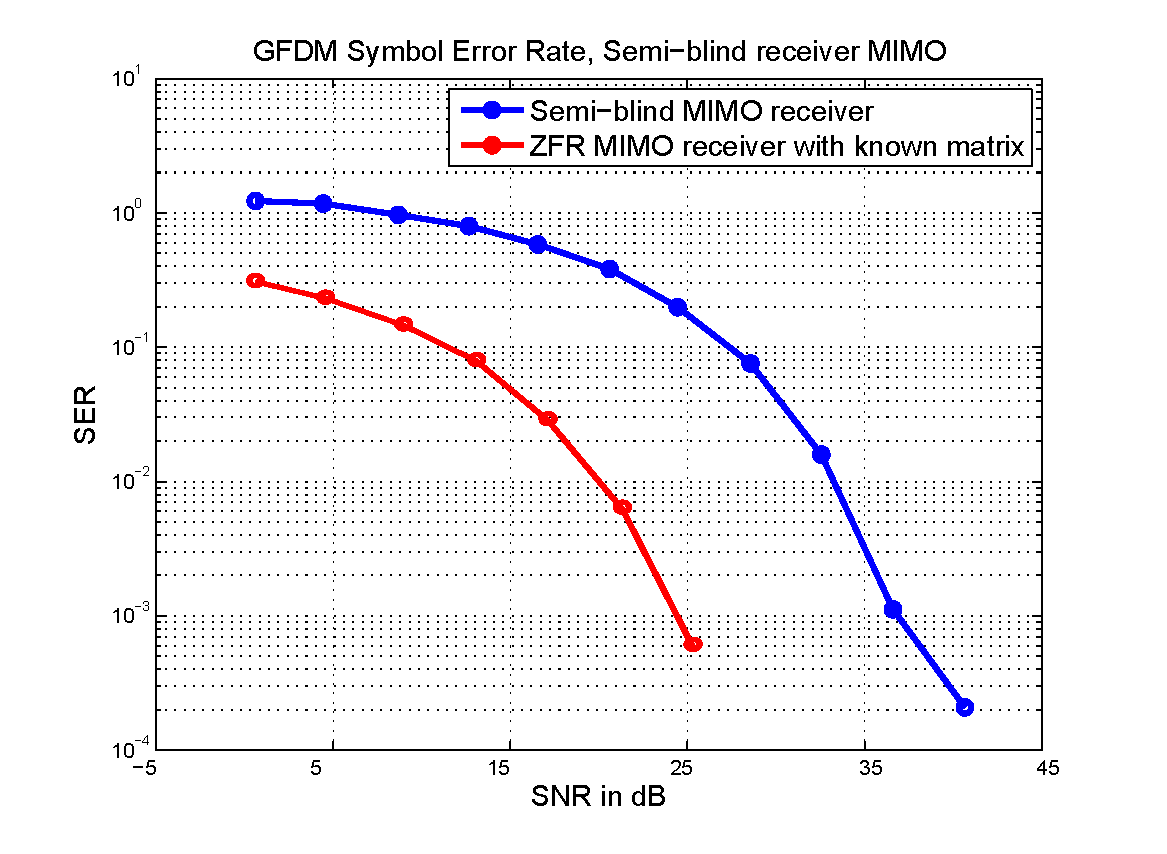
\includegraphics[width=0.9\columnwidth]{MIMO_SER_1.eps}
%\caption{\textit{\label{fs_m_0}SER for the channel orthogonalization in GFDM MIMO}}
%\end{figure}
\subsection{Scenario 2.1}
The performance results of the $\mathcal{A}$ search algorithm are obtained through simulation. The parameters of the system are tabulated in Table \ref{tab:m_table_1}.   
The GFDM system is simulated in the AWGN channel without coding. QPSK modulation scheme is used. The number of sub-carriers was $F=16$, samples for each symbol was $T/T_s=F$ The block size was $T_s=5$. The root-raised cosine filter was used with  roll-off factor $\alpha=0.5$. The selection coefficients was chosen mode two products between identity matrix in the first and third dimension with random integer values array.   The results of the GFDM performance is presented in the two plots, at first is shown the reconstruction error for the $\mathbf{A}$ fig. \ref{fig:fs_m_1}, at second is shown the SER in comparison with the case  if $\mathbf{a}=\mathbf{1}$ with the zero-forced receiver fig. \ref{fig:fs_m_2}. 
\begin{table}[H]
\caption{\label{tab:m_table_1}GFDM simulation parameters.Scenario 2.1}
\begin{center}
\begin{tabular}{|c|c|c|}
\hline
Parameter & Variable & GFDM \\
\hline
\hline
Transmit antennas &$M_t$&2 \\
\hline
Receive antennas &$M_r$&2 \\
\hline
Modulation scheme & $\mu$ & QPSK \\
\hline
Samples per symbol & $T/T_s$ & 16 \\
\hline
Sub-carriers&$F$&16 \\
\hline
Block size& $T_s$  &5 \\
\hline
Filter type&  &RRC \\
\hline
Roll-off-factor&$\alpha$  &0.5 \\
\hline
Sub-carrier coefficients& $\mathbf{a}_i$ & $unif(0,1)$ \\
\hline
Channel& $h$ &Flat-fading \\
\hline
Cyclic Prefix&  & No \\
\hline
Transmission&  & Uncoded\\
\hline
Decomposition rank& $rank$ & 25\\
\hline
\end{tabular}
\end{center}
\end{table}
\begin{figure}[H]
\centering
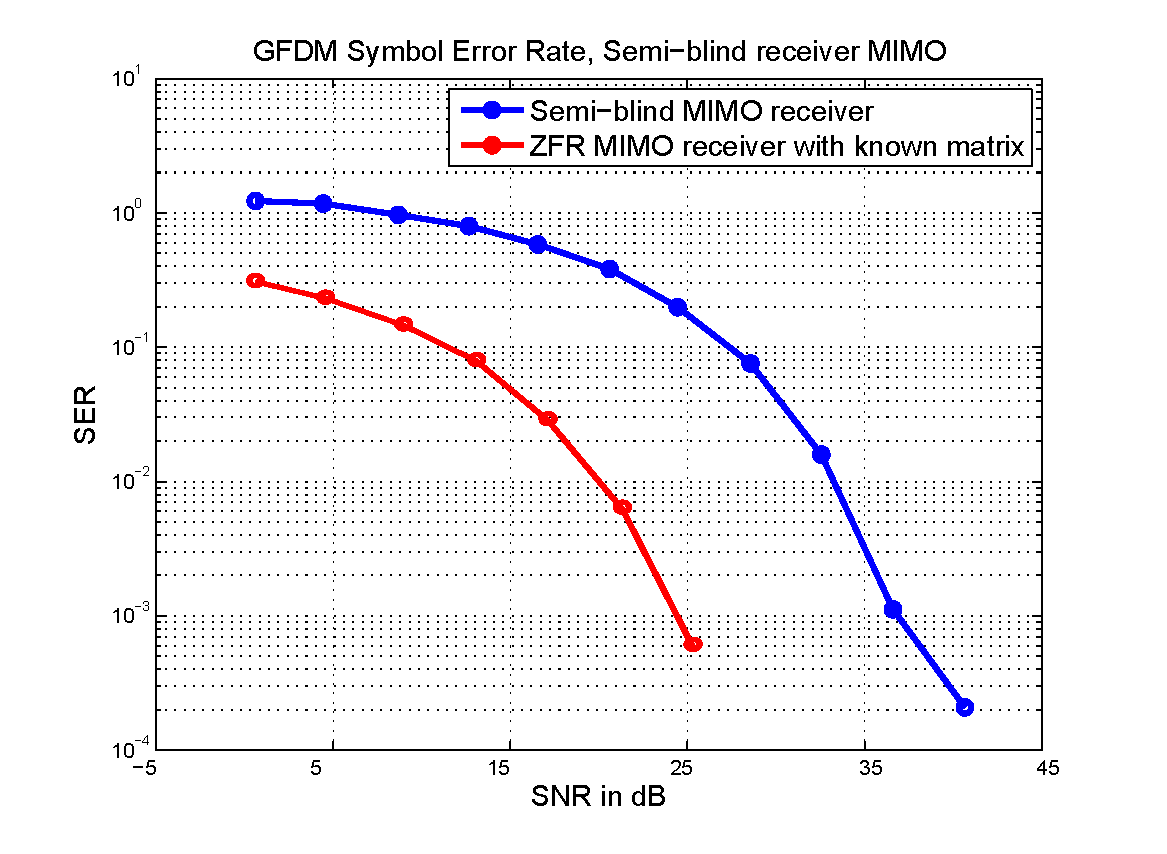
\includegraphics[width=0.9\columnwidth]{MIMO_SER_1.eps}
\caption{\label{fig:fs_m_1}\textit{SER dependency for the semi-blind MIMO receiver and ZF receiver with known channel}}
\end{figure}
\begin{figure}[H]
\centering
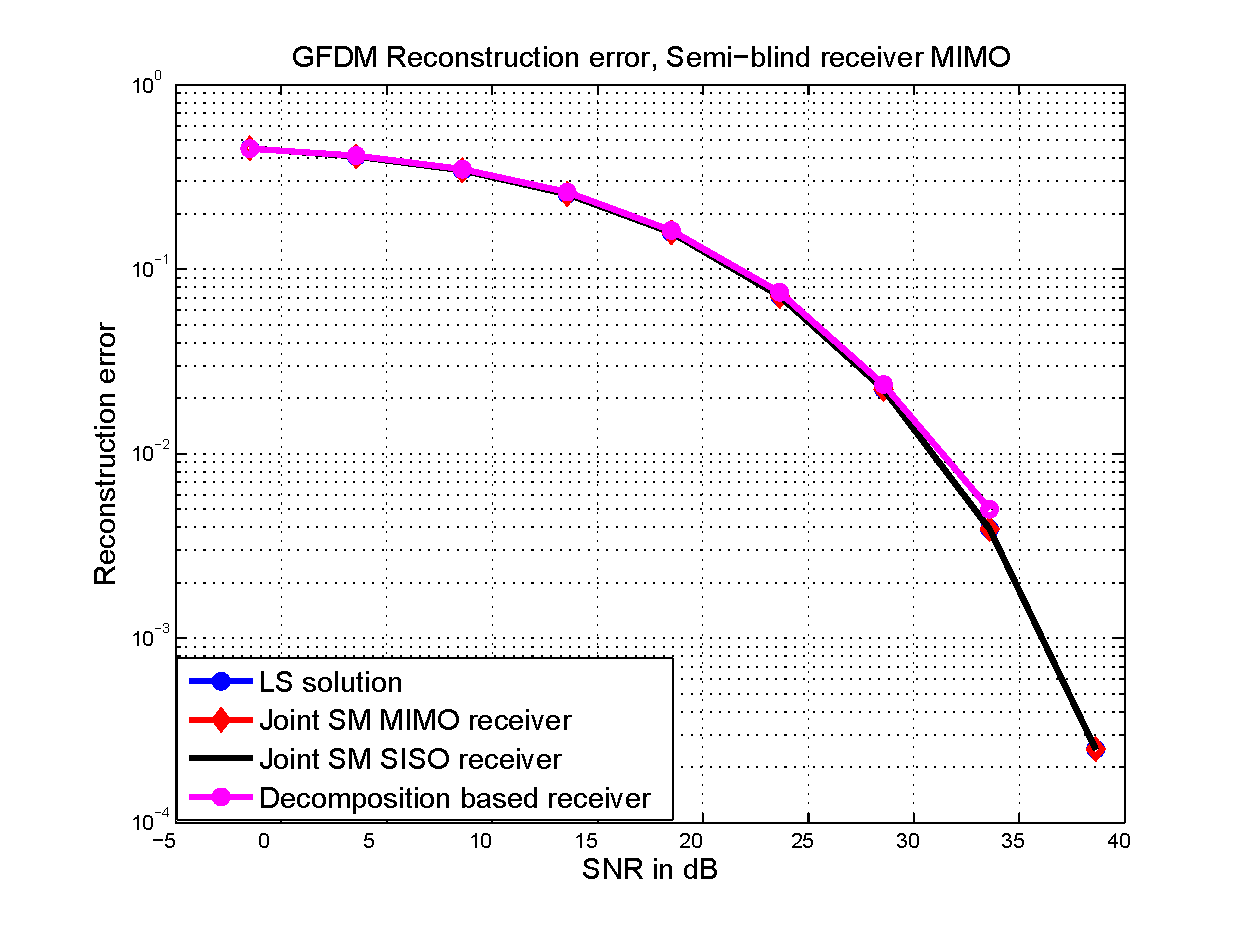
\includegraphics[width=0.9\columnwidth]{SM_RE_MIMO.eps}
\caption{\label{fig:fs_m_2}\textit{Reconstruction error for the sub-carrier estimation approaches}}
\end{figure}
\subsection{Scenario 2.2}
 \begin{table}[H]
\caption{\label{tab:m_table3}GFDM simulation parameters.Scenario 2.2}
\begin{center}
\begin{tabular}{|c|c|c|}
\hline
Parameter & Variable & GFDM \\
\hline
\hline
Modulation scheme & $\mu$ & QPSK \\
\hline
Samples per symbol & $T/T_s$ & 16 \\
\hline
Sub-carriers&$F$&16 \\
\hline
Block size& $T_s$  &5 \\
\hline
Transmit antennas &$M_t$&2 \\
\hline
Receive antennas &$M_r$&2 \\
\hline
Filter type&  &RRC \\
\hline
Roll-off-factor&$\alpha$  &1 \\
\hline
Length of the channel& $L+1$ & 12 \\
\hline
Channel& $h$ & Ped-A \\
\hline
Cyclic Prefix&  & No \\
\hline
Transmission&  & Uncoded\\
\hline
\end{tabular}
\end{center}
\end{table}
The GFDM system semi-blind receiver in the MIMO system is simulated in the frequency selective channel without coding. QPSK modulation scheme is used. The channel was generated in the two steps. At the first step was generated flat frequency channel matrix $\mathbf{H}$ with zero-mean circularly symmetric complex Gaussian random values. At the second step for each values of the matrix $\mathbf{H}$ generated the tensor $\mathcal{H}$ with time filter coefficients for each transmission link. At the end each slice of the tensor $\mathcal{H}$ is element-wise multiplied with $\mathbf{H}$. The number of the receive and transmit antennas was $M_r=M_t=3$.  The number of sub-carriers was $F=8$, samples for each symbol was $T/T_s=F$ The block size was $T_s=3$. The root-raised cosine filter was used with roll-of-factor $\alpha=1$. The length of the channel equal to $L+1=4$. The experiment setup is presented in the table \ref{tab:m_table3}. The results of the GFDM performance is presented in the two plots, at first \eqref{fig:fs_m_3} is shown the SER in comparison with the case  if receiver know the original channel and use the Zero-Forced receiver and with case for different number of unknown symbols in one transmission block. At second figure \eqref{fig:fs_m_4} is shown the reconstruction error for the channel values \eqref{sim:eq_m_1}.\begin{align}
R_e=\frac{\mid\mid\mathbf{A-\widehat{A}}\mid\mid^2}{\mid\mid\mathbf{A}\mid\mid^@}
\label{sim:eq_m_1}
\end{align}
\begin{figure}[H]
\centering
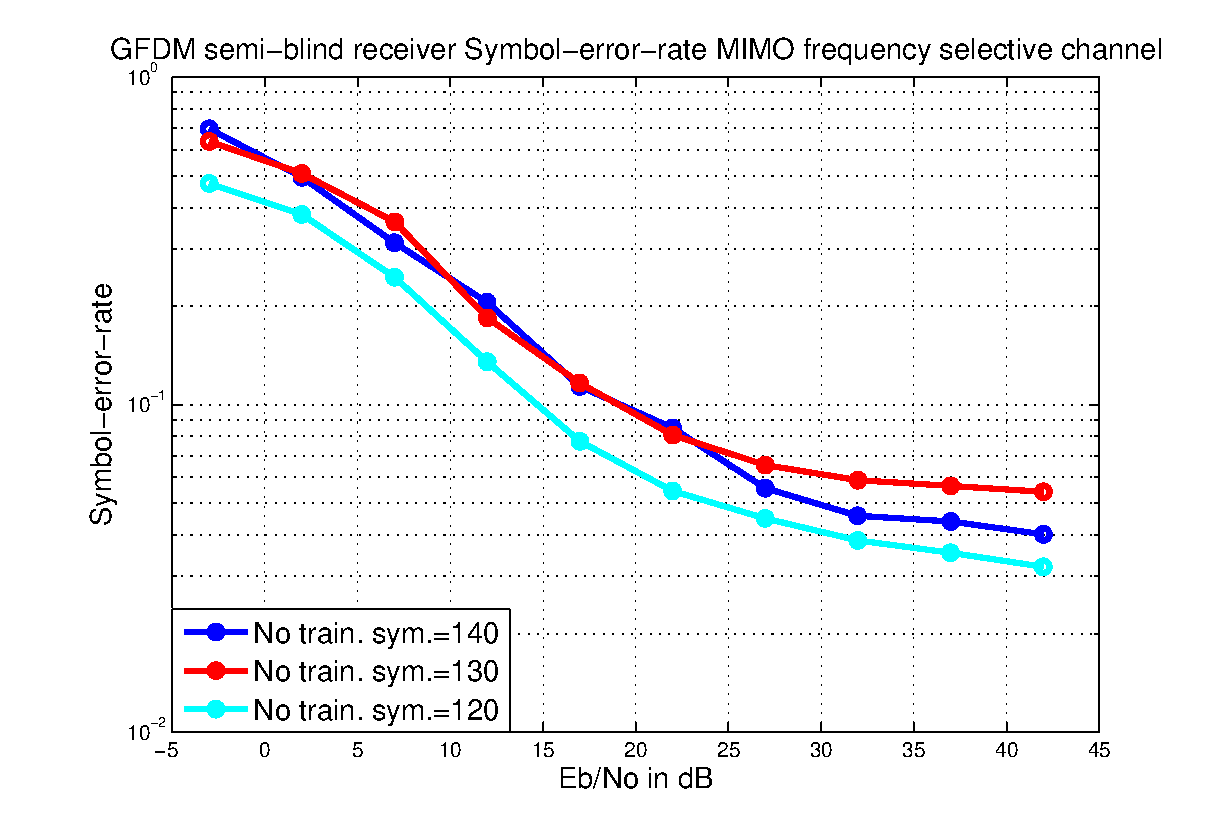
\includegraphics[width=0.9\columnwidth]{SM_MIMO_SER_ALS.eps}
\caption{\textit{SER for the semi-blind MIMO receiver with different number of known symbols}}
\label{fig:fs_m_3}
\end{figure}
\begin{figure}[H]
\centering
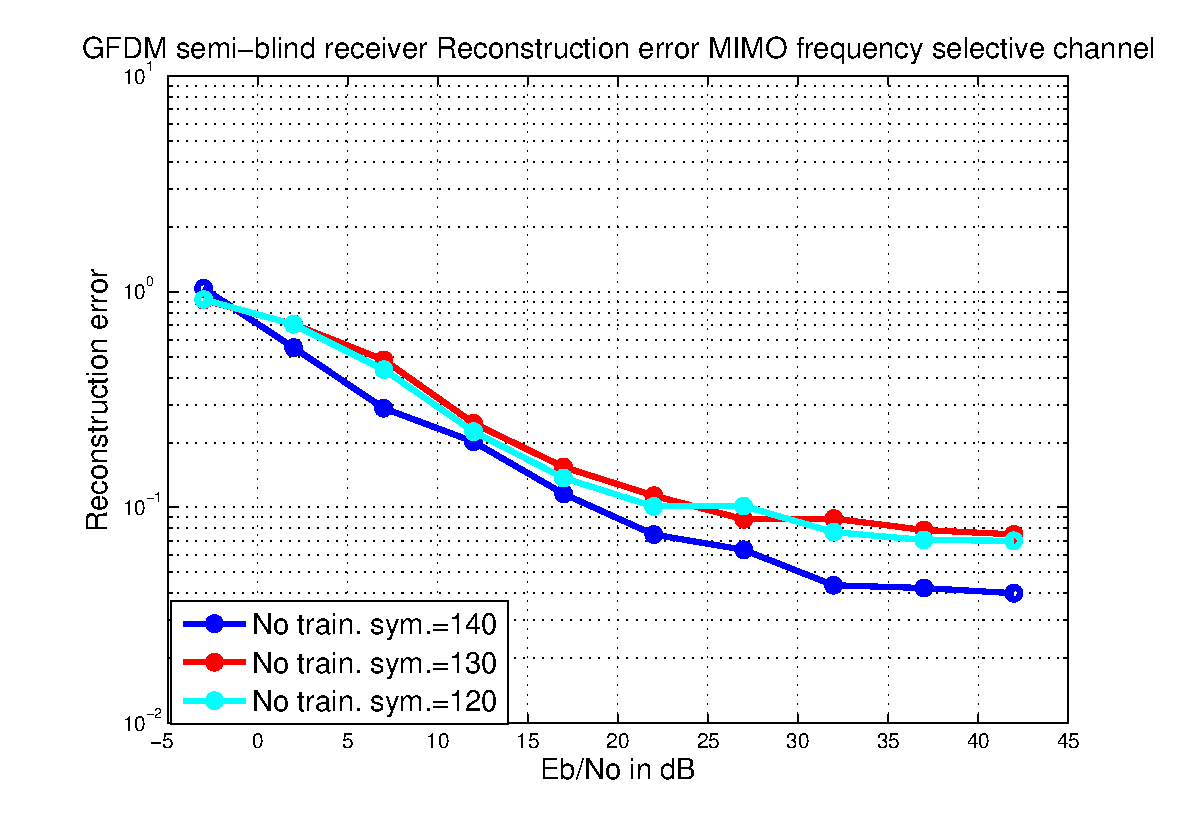
\includegraphics[width=0.9\columnwidth]{SM_MIMO_RE_ALS.eps}
\caption{\textit{Channel reconstruction error for the semi-blind MIMO receiver with different number of known symbols}}
\label{fig:fs_m_4}
\end{figure}
\subsection{Scenario 2.3}
The GFDM system Newton based semi-blind receiver in the MIMO system is simulated in the frequency selective channel without coding. QPSK modulation scheme is used. The channel was generated in the two steps. At the first step was generated flat frequency channel matrix $\mathbf{H}$ with zero-mean circularly symmetric complex Gaussian random values. At the second step for each values of the matrix $\mathbf{H}$ generated the tensor $\mathcal{H}$ with time filter coefficients for each transmission link. At the end each slice of the tensor $\mathcal{H}$ is element-wise multiplied with $\mathbf{H}$. The number of the receive and transmit antennas was $M_r=M_t=3$.  The number of sub-carriers was $F=8$, samples for each symbol was $T/T_s=F$ The block size was $T_s=3$. The root-raised cosine filter was used with roll-of-factor $\alpha=1$. The length of the channel equal to $L+1=4$. The experiment setup is presented in the table \ref{tab:m_table3}. The results of the GFDM performance is presented in the two plots, at first \eqref{fig:fs_m_5} is shown the SER in comparison with the case  if receiver know the original channel and use the Zero-Forced receiver and with case for different number of unknown symbols in one transmission block. At second figure \eqref{fig:fs_m_6} is shown the reconstruction error for the channel values. The reconstruction error is defined in the \eqref{sim:eq_m_2}
\begin{align}
R_e=\frac{\mid\mid\mathbf{h-\widehat{h}}\mid\mid^2}{\mid\mid\mathbf{h}\mid\mid^@}
\label{sim:eq_m_2}
\end{align}
\begin{figure}[H]
\centering
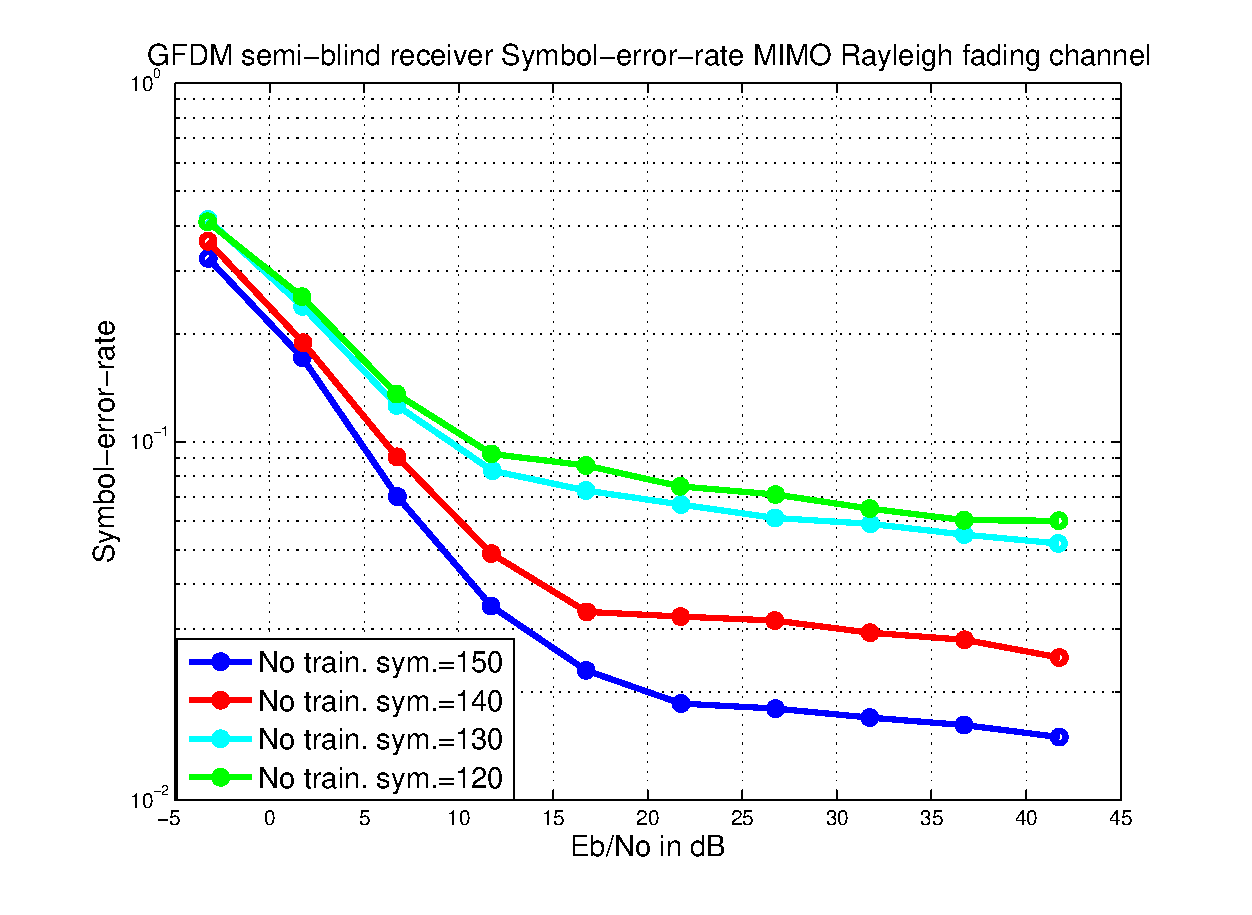
\includegraphics[width=0.9\columnwidth]{SM_MIMO_SER_N.eps}
\caption{\textit{SER for the semi-blind MIMO receiver with different number of known symbols}}
\label{fig:fs_m_5}
\end{figure}
\begin{figure}[H]
\centering
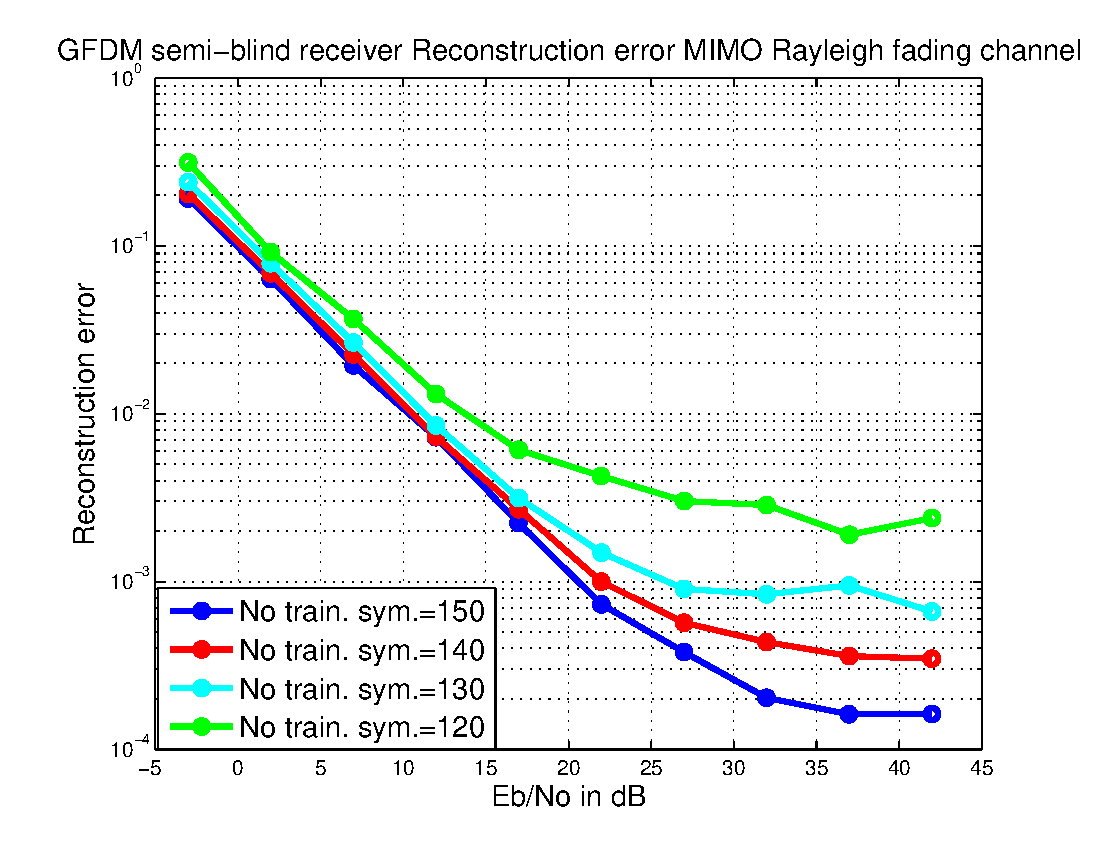
\includegraphics[width=0.9\columnwidth]{SM_MIMO_RE_N.eps}
\caption{\textit{Channel reconstruction error for the semi-blind MIMO receiver with different number of known symbols}}
\label{fig:fs_m_6}
\end{figure}
\section{Conclusion}\label{sec:CMIMO}

As conclusion for the second experiment with frequency coefficient selection approach in the MIMO case, we can see that algorithm decrease performance for 5-6 dB in comparison with system where the frequency coefficients known fig. \ref{fig:fs_m_2}. Decrease in performance come from the non-convenient coefficient selection way. The coefficients were chosen as $1$ if the resulting $abs(a_1)$ value is higher that $0.5$. There are better solutions to increase performance of the algorithm with the predefined information at the receiver.

We explained three frequency coefficients estimation approaches. As we can see from the result at the fig.\ref{fig:fs_m_3} all of them has the same result. Even the approximated solution based on the SISO model show the same performance. Due to that fact there is no difference with algorithm to choose. It should be noted that the joint MIMO algorithm allow to also the symbol estimation. Other algorithms can't estimate the symbols in the received data and work only if transmission block equal to the number of symbols in each subcarrier. There is one additional disadvantage of the Decomposition based approach, which doesn't converge with some initial points. Due to that fact decomposition based approach is less reliable than other algorithms.  The overall conclusion over the frequency selection coefficient algorithms we can say that spectrum sensing approach is applicable in the  MIMO case too. The system may use different subcarrier antennas for each transmit antenna and the receiver can estimate them. The performance loss is similar to the SISO case, but number of the time-slots decrease significantly in comparison with the SISO case. In the paper is explained very simple approaches to coefficients estimation.  Performance of the algorithm can be implemented in more efficient way without huge performance loss. We doesn't use any pre-processing and post-processing steps to increase performance.
 
%The main assumption of the SISO semi-blind based approach is error spread between transmit antennas. We ignored unknown values because unknown symbols at the receiver doesn't used. Repetition of the algorithm for the each transmit antenna allow to estimate coefficients for the sub-carrier selection matrix. Assumption is not applied for the time slots due to the overlapping and the receiver estimates the coefficient approximately. The error depends from the difference between sub-carrier selection coefficients in the each transmit antenna due to the time slot mixing in the GFDM systems. The SISO semi-blind based approach is the most expensive algorithm in comparison with others. The receiver can estimate parallel solution for the each sub-carrier selection coefficient corresponding to the each transmit antenna. The parallel solution decreases iteration time of the approach.
%The algorithm based on the least squares solution achieve the better results. The approach doesn't have assumptions in the mathematical model  for the GFDM system. But the least squares solution is very sensitive to the condition number of the matrix. The least squares solution is expensive too.
%The decomposition based approach of the unfolding multiplication with the matrix decrease size of the problem.  There is trade of between complexity of the task and calculation of the optimization process. Each iteration contain the matrix inversion inside. The matrix to invert change every iteration change from iteration to iteration.
%We can see that result of the all three algorithms is the same. There is significant difference for the decomposition based approach if we use the mean value metric. because we can choose bas initial point. Therefore we used the median value metric.

Next experiment is the semi-blind receiver channel and the symbol estimation over frequency selective channel with Rayleigh fading. The pedestrian-A channel was assumed in the each of the antennas. The experiment was done for the number of possible known symbols which have solution for the problem statement. The result for the SER if shown in the fig. \ref{fig:fs_m_3}. We can see from the plot, that performance of the algorithm is weak. With high SNR the algorithm has only $10^{-2}$ SER, which is very high value. This behavior is explained with the very bad conditioning of the channel matrix. The additional fact is the low performance of the Rayleigh fading channel itself. We can implement the more convenient ways of the algorithm to avoid such low performance. There is additional investigation about typical real channel should be done. We can see from the fig. the channel estimation has the upper bound of precision. We can say that algorithm has the same performance from the $30$ dB. There is significant dependency from the channel estimation precision as we can see here. The upper bound of the channel estimation doesn't allow increasing performance with higher SNR. As conclusion for the ALS based semi-blind receiver we can say that algorithm isn't provide full performance and they pre-processing and post-processing steps should be applied to increase the performance. This behavior will be investigated in the future work.
The last experiment show performance of the Newton based semi-blind receiver over the frequency selective Rayleigh fading channel. The fig.\eqref{fig:fs_m_5} show the performance of the algorithm in the symbol estimation. As we can see here the algorithm has the upper bound in the performance and doesn't allow to decrease the SER lower than $10^{-2}$. This behavior doesn't connect with error in the channel estimation, because the error in the channel estimation is upper bounded with much higher SNR and have precision near to the $10^{-3}$/ The main reason for this behavior is the high condition number of the Jacobian matrix. To implement the more precise and regularized solution the BFGS of Levenberg-Marquardt algorithm must be applied. We can see from the results, that there is significant dependency between the  number of the training symbols and performance of the system. The number of the training symbols is high due to the high number of estimated channel variables.The fig.\eqref{fig:fs_m_6} show the performance of the algorithm in the channel estimation. We can see that precision of the algorithm is high and algorithm estimates the channel with precision up to $10^{-3}$ reconstruction error. There are disadvantages of the algorithm which connected with bad conditioning and the computational complexity. The additional approaches must be investigated to overcome them. As conclusion for this algorithm we can propose two statements:
\begin{itemize}
\item Performance of the algorithm weak for the symbol estimation
\item Performance of the algorithm applicable for the channel estimation
\item The algorithm must use the regularizing approach.
\end{itemize}




%As we can see here, there is one optimal point in symbol estimation. The less unknown symbols in the block increase the SNR, whether the higher number of unknown symbols decrease performance of the approach. The solution where number of unknown symbols equal to $8$ show the closest result to the original GFDM system with the same block size, known channel and zero forced receiver. The channel reconstruction error has the similar behaviour and show the optimal point in the same number of unknown symbols. Important fact is that reconstruction error for the maximal and minimal number of unknown have different behaviour in comparison with the SISO model. But this behaviour also show the convexity of the performance function for the number of unknown symbols as variable. The different block size should have different optimal value of the unknown symbols, but the average performance must be the worse from the known channel system due to the higher energy per bit with same performance. 
\cleardoublepage
\addcontentsline{toc}{chapter}{Список литературы}
\bibliographystyle{utf8gost705u}  
\bibliography{art1} 
\cleardoublepage
\end{document}

%\selectlanguage{russian}